\documentclass[11pt,a4paper,oneside]{report}

% --- Codificación e idioma ---
\usepackage[utf8]{inputenc}
\usepackage[T1]{fontenc}
\usepackage[spanish,es-tabla,es-nodecimaldot]{babel}
\usepackage{csquotes}

% --- Tipografía y microtipografía ---
\usepackage{lmodern}
\usepackage{microtype}

% --- Márgenes y geometría ---
\usepackage[
  top=2.5cm,
  bottom=2.5cm,
  left=3.0cm,
  right=2.5cm
]{geometry}
\usepackage{setspace}
\onehalfspacing
\setlength{\parskip}{0.45em}
\setlength{\parindent}{0pt}

% --- Encabezados y pies de página ---
\usepackage{fancyhdr}
\pagestyle{fancy}
\fancyhf{}
\fancyhead[L]{\small\textit{Tablero de organización con tarjetas inteligentes}}
\fancyhead[R]{\small\textit{ITBA}}
\fancyfoot[C]{\thepage}
\renewcommand{\headrulewidth}{0.4pt}

% --- Gráficos, tablas y colores ---
\usepackage{graphicx}
\usepackage{float}
\usepackage{booktabs}
\usepackage{longtable}
\usepackage{tabularx}
\usepackage{array}
\usepackage{xcolor}
\usepackage[table]{xcolor}
\usepackage{caption}
\captionsetup{font=small,labelfont=bf,justification=centering}

% --- Código y formato técnico ---
\usepackage{enumitem}
\usepackage{listings}
\lstset{
  basicstyle=\ttfamily\small,
  breaklines=true,
  frame=single,
  backgroundcolor=\color{gray!8}
}

% --- Enlaces y marcadores PDF ---
\usepackage[hidelinks,breaklinks=true]{hyperref}

% --- Bibliografía IEEE en español (Disposición ITBA 645/2016 y 882/2019) ---
\usepackage[
  backend=biber,
  style=ieee,
  sorting=none,
  language=spanish
]{biblatex}
\addbibresource{referencias.bib}

% --- Ajuste de títulos de capítulo sin palabra "Capítulo X" si se desea estilo informe ---
\usepackage{titlesec}
\titleformat{\chapter}[hang]{\normalfont\LARGE\bfseries}{\thechapter.}{0.8em}{}
\titlespacing*{\chapter}{0pt}{-15pt}{15pt}

% --- Estilo unificado para tablas de esquemas de base de datos (Tablas 5.1 a 5.10) ---
\newenvironment{tablacoleccion}[2]{%
  \begingroup
  \footnotesize
  \setlength{\tabcolsep}{4.5pt}%
  \renewcommand{\arraystretch}{1.35}%
  \rowcolors{2}{gray!7}{white}%
  \longtable{
    >{\ttfamily\raggedright\arraybackslash}p{\dimexpr 0.25\textwidth - 2\tabcolsep\relax}
    >{\raggedright\arraybackslash}p{\dimexpr 0.17\textwidth - 2\tabcolsep\relax}
    >{\raggedright\arraybackslash}p{\dimexpr 0.17\textwidth - 2\tabcolsep\relax}
    >{\raggedright\arraybackslash}p{\dimexpr 0.41\textwidth - 2\tabcolsep\relax}
  }
  \toprule
  \rowcolor{gray!18}
  \normalfont\bfseries Campo & \bfseries Tipo BSON & \bfseries Indexado & \bfseries Descripción \\
  \midrule
  \endfirsthead
  \toprule
  \rowcolor{gray!18}
  \normalfont\bfseries Campo & \bfseries Tipo BSON & \bfseries Indexado & \bfseries Descripción \\
  \midrule
  \endhead
  \midrule
  \multicolumn{4}{r}{\textit{\scriptsize Continúa en la página siguiente...}} \\
  \endfoot
  \bottomrule
  \caption{#1}
  \label{#2}
  \endlastfoot
}{%
  \endlongtable
  \endgroup
}

% --- Estilo unificado para tablas de endpoints de 3 columnas ---
\newenvironment{tablaendpoints}[2]{%
  \begingroup
  \footnotesize
  \setlength{\tabcolsep}{4.5pt}%
  \renewcommand{\arraystretch}{1.35}%
  \rowcolors{2}{gray!7}{white}%
  \longtable{
    >{\bfseries\raggedright\arraybackslash}p{\dimexpr 0.18\textwidth - 2\tabcolsep\relax}
    >{\ttfamily\raggedright\arraybackslash}p{\dimexpr 0.35\textwidth - 2\tabcolsep\relax}
    >{\raggedright\arraybackslash}p{\dimexpr 0.47\textwidth - 2\tabcolsep\relax}
  }
  \toprule
  \rowcolor{gray!18}
  \textbf{Método} & \normalfont\bfseries Ruta & \bfseries Función \\
  \midrule
  \endfirsthead
  \toprule
  \rowcolor{gray!18}
  \textbf{Método} & \normalfont\bfseries Ruta & \bfseries Función \\
  \midrule
  \endhead
  \midrule
  \rowcolor{white}
  \multicolumn{3}{r}{\textit{\scriptsize Continúa en la página siguiente...}} \\
  \endfoot
  \bottomrule
  \caption{#1}
  \label{#2}
  \endlastfoot
}{%
  \endlongtable
  \endgroup
}

% --- Estilo unificado para tablas de endpoints de 4 columnas (con Rol Mínimo) ---
\newenvironment{tablaendpointsrol}[2]{%
  \begingroup
  \footnotesize
  \setlength{\tabcolsep}{4.5pt}%
  \renewcommand{\arraystretch}{1.35}%
  \rowcolors{2}{gray!7}{white}%
  \longtable{
    >{\bfseries\raggedright\arraybackslash}p{\dimexpr 0.12\textwidth - 2\tabcolsep\relax}
    >{\ttfamily\raggedright\arraybackslash}p{\dimexpr 0.36\textwidth - 2\tabcolsep\relax}
    >{\raggedright\arraybackslash}p{\dimexpr 0.36\textwidth - 2\tabcolsep\relax}
    >{\raggedright\arraybackslash}p{\dimexpr 0.16\textwidth - 2\tabcolsep\relax}
  }
  \toprule
  \rowcolor{gray!18}
  \textbf{Método} & \normalfont\bfseries Ruta & \bfseries Función & \bfseries Rol Mínimo \\
  \midrule
  \endfirsthead
  \toprule
  \rowcolor{gray!18}
  \textbf{Método} & \normalfont\bfseries Ruta & \bfseries Función & \bfseries Rol Mínimo \\
  \midrule
  \endhead
  \midrule
  \rowcolor{white}
  \multicolumn{4}{r}{\textit{\scriptsize Continúa en la página siguiente...}} \\
  \endfoot
  \bottomrule
  \caption{#1}
  \label{#2}
  \endlastfoot
}{%
  \endlongtable
  \endgroup
}

\begin{document}

% 1. Carátula obligatoria ITBA
\begin{titlepage}
  \singlespacing
  \setlength{\parskip}{0pt}
  \centering

  % 1) Nombre y logo de la universidad
  
\includegraphics[height=2.6cm,keepaspectratio]{figuras/logo_itba.png}\par
  \vspace{0.5cm}
  {\Large\bfseries INSTITUTO TECNOLÓGICO DE BUENOS AIRES – ITBA\par}
  \vspace{0.25cm}
  % 2) Escuela a la cual pertenece la carrera
  {\large\bfseries ESCUELA DE INGENIERÍA Y GESTIÓN\par}

  \vspace{\stretch{1.2}}
  \rule{\textwidth}{0.8pt}\par\vspace{0.45cm}
  % 3) Título del trabajo
  {\Huge\bfseries Tablero de organización con tarjetas inteligentes\par}
  \vspace{0.45cm}\rule{\textwidth}{0.8pt}\par

  \vspace{\stretch{1.2}}
  % 4) Datos de los alumnos (apellido, nombre y legajo)
  {\large\bfseries AUTORES:\par}
  \vspace{0.3cm}
  {\large
    Torlaschi, Patrick Luca \quad (Legajo: 62273)\\[0.2em]
    Noceda, Tobías Martín \quad (Legajo: 63422)\\[0.2em]
    Raiti, Tomás Ignacio \quad (Legajo: 62887)\par
  }

  \vspace{0.8cm}
  % 5) Datos del tutor
  {\large\bfseries Tutor:\par}
  \vspace{0.2cm}
  {\large Botti, Federico\par}

  \vspace{\stretch{1.5}}
  % 6) Leyenda indicativa del título al que se aspira
  {\large\bfseries TRABAJO FINAL PRESENTADO PARA LA OBTENCIÓN DEL TÍTULO DE INGENIERO EN INFORMÁTICA\par}

  \vspace{0.7cm}
  % 7) Lugar y fecha de presentación
  {\large Ciudad Autónoma de Buenos Aires, 16 de octubre de 2026}
\end{titlepage}

% 2. Índice general, índice de tablas e índice de figuras
\pagenumbering{roman}
\tableofcontents
\clearpage
\listoffigures
\listoftables
\clearpage

% Nota preliminar del documento
% \noindent\textit{Nota: salvo indicación en contrario, todas las figuras y tablas del presente documento son de elaboración propia.}
\vspace{1em}

% 3. Cuerpo del informe (numeración arábiga)
\pagenumbering{arabic}
% !TEX root = ../main.tex
\chapter{Explicación del Proyecto}

\section{Contexto}
En la actualidad, la información relevante para la toma de decisiones se encuentra distribuida en múltiples plataformas y servicios: precios de mercado, estados de sistemas, tickets de soporte, repositorios de código, datos de viajes, entre otros. Esta dispersión obliga a los usuarios a alternar constantemente entre herramientas, perdiendo tiempo y contexto en el proceso. Si bien existen soluciones de organización como Notion, Trello o dashboards personalizados, ninguna combina la flexibilidad visual de un tablero libre con la capacidad de consumir datos en tiempo real de fuentes externas arbitrarias.

El problema afecta a perfiles de usuario muy distintos. Una persona que sigue sus finanzas consulta a diario cotizaciones, tasas y saldos en sitios diferentes; quien planifica un viaje compara precios de vuelos, alojamientos y el pronóstico del clima del destino; un equipo de desarrollo controla el estado de sus repositorios, issues y despliegues; y, cada vez con mayor frecuencia, los usuarios de asistentes de inteligencia artificial necesitan que esos asistentes recuerden información y la mantengan organizada entre conversaciones.

Se trata de información dinámica, que cambia en cuestión de minutos u horas; heterogénea, ya que proviene de fuentes con formatos distintos; dispersa en servicios que exponen cada uno su propia API. Además, en muchos casos, es privada, por lo que acceder a ella requiere credenciales o la autorización del usuario. Hoy, la forma habitual de seguirla consiste en abrir varias pestañas o aplicaciones, refrescarlas manualmente y copiar los datos relevantes a una nota o planilla. Este proceso consume tiempo, produce datos que quedan desactualizados en cuanto se copian y no permite ver las relaciones entre ellos, como el efecto de la cotización del dólar sobre el presupuesto de un viaje.

Para resolver este problema, hace falta un espacio que reúna en un mismo lugar información de fuentes diversas, la mantenga actualizada sin intervención del usuario y permita expresar las relaciones entre los datos.

El proyecto surge en este contexto como una herramienta web que unifica la organización visual de información con la actualización automática de datos provenientes de APIs externas. Inspirado en la metáfora del pizarrón de corcho, popularizada en series policiales donde las tarjetas se conectan con hilos para revelar relaciones, el sistema permite al usuario construir tableros inteligentes donde cada tarjeta representa una fuente de información viva, y los hilos entre ellas expresan relaciones, dependencias o secuencias temporales. Los tableros pueden compartirse para trabajar sobre ellos en tiempo real, y un servidor MCP permite que los agentes de inteligencia artificial los utilicen para guardar y consultar sus propias memorias, que el usuario puede ver y editar como cualquier otra tarjeta.

\section{Objetivo}
El objetivo general del proyecto es desarrollar una aplicación web que permita reunir en tableros visuales información proveniente de fuentes externas, mantenerla actualizada de forma automática y expresar las relaciones entre los datos, ofreciendo además a los agentes de inteligencia artificial un medio para gestionar sus memorias sobre la misma herramienta.

Para alcanzarlo, se plantearon los siguientes objetivos específicos:
\begin{itemize}
  \item Construir un lienzo en el que las tarjetas puedan crearse, moverse y conectarse mediante hilos.
  \item Ofrecer un catálogo de integraciones predefinidas que no requieran conocimientos técnicos y permitir conectar tarjetas a APIs personalizadas.
  \item Actualizar el contenido de cada tarjeta de forma automática, según la frecuencia configurada.
  \item Almacenar de forma segura las credenciales necesarias para acceder a fuentes privadas.
  \item Permitir compartir tableros y reflejar en tiempo real los cambios de todos sus miembros.
  \item Exponer los tableros a los agentes de inteligencia artificial mediante un servidor MCP, para que gestionen sus memorias como tarjetas.
\end{itemize}

\section{Estado del arte}
Existen en el mercado distintas herramientas que resuelven parte del problema descrito. A continuación se presentan las principales, y la Tabla~\ref{tab:comparacion_herramientas} las compara según un mismo conjunto de criterios: tipo de tecnología, problema que resuelve, tipo de solución, integración de datos dinámicos y representación explícita de relaciones.

\begin{itemize}
  \item \textbf{Notion:} Permite generar wikis estructuradas con bases de datos relacionales para poder relacionarlas. Excelentes para documentación jerarquizada y colaboración en equipo. Las relaciones entre nodos (wikis) existen, pero son fundamentalmente lineales, no se ven en un grafo de relaciones gráfico y explícito, está implícito en links que permiten la navegación sin tener todo el contexto de relaciones. No tienen actualización dinámica de datos en tiempo real \cite{notion_about, morton2025}.
  \item \textbf{Miro, FigJam, Mural:} Pizarras visuales colaborativas infinitas. Excelentes para brainstorming \cite{mural_brainstorming} y diagramación libre, pero los nodos son formas estáticas y muestran toda la información en pantalla, saturando la visual y perdiendo el foco en las relaciones. No tienen integración nativa con datos en vivo ni semántica de grafo real \cite{miro_about, yamashita2021, morton2025}.
  \item \textbf{Kumu, Gephi:} Son herramientas de visualización y análisis de grafos \cite{wills2026}. Gephi es especialmente potente para análisis de redes, pero es un software orientado a análisis de datos estáticos \cite{ouestware2025}. Kumu permite grafos dinámicos pero sin integración fluida con APIs externas \cite{kumu_manifesto}.
  \item \textbf{Trello:} Plataforma de gestión de tareas basada en el modelo Kanban, organizada en tableros, listas y tarjetas. Es excelente para el seguimiento de flujos de trabajo y la colaboración en equipo gracias a su simplicidad. Sin embargo, su estructura es rígidamente columnar: las tarjetas se agrupan en listas secuenciales y no existe la noción de relaciones explícitas ni de hilos entre ellas, por lo que no permite representar dependencias o conexiones arbitrarias en un grafo. Si bien admite la incorporación de automatizaciones y extensiones (Power-Ups), las tarjetas son contenedores de información estática y no ofrecen actualización dinámica de datos en tiempo real desde fuentes externas \cite{trello_about}.
  \item \textbf{Personal knowledge graphs:} Los grafos de información personal (PKGs) son una representación estructurada de información sobre entidades relacionadas personalmente con un individuo, como personas, lugares, objetos y eventos \cite{velitchkov2023}. Aunque hay un abundante número de trabajos desarrollados alrededor del tema, la mayoría de los trabajos se limitan a un estudio teórico del tema, sin expandir en la posibilidad de implementarse como una herramienta digital o producto, o limitándose a un número finito de entidades, como personas, lugares y eventos \cite{new2026, pavlyshyn2024, rasmus2024}.
  \item \textbf{Inteligencia artificial:} En 2019, dos ingenieros de Google publicaron un artículo sobre los PKG, en el cual incluían ilustraciones de escenarios donde un asistente virtual podría beneficiarse del uso de un grafo de conocimiento para así contestar consultas complejas de manera más personalizada y con mayor precisión. Hace 7 años tal tecnología se consideraba ciencia ficción, pero con los avances que vio el mundo de la inteligencia artificial en la última década, estos ``ejemplos motivacionales'' pasaron de ser ideas de películas a la tecnología del presente \cite{balog2019}.
\end{itemize}

\begin{table}[H]
  \centering
  \footnotesize
  \setlength{\tabcolsep}{4.5pt}
  \renewcommand{\arraystretch}{1.35}
  \newcolumntype{L}[1]{>{\raggedright\arraybackslash\hsize=#1\hsize}X}
  \rowcolors{2}{gray!7}{white}
  \begin{tabularx}{\textwidth}{
    >{\bfseries}L{0.95}
    L{1.05}
    L{0.95}
    L{1.05}
    L{1.00}
    L{1.00}
  }
    \toprule
    \rowcolor{gray!18}
    \textbf{Herramienta} & \textbf{Tecnología} & \textbf{Problema que resuelve} & \textbf{Tipo de solución} & \textbf{Datos dinámicos} & \textbf{Relaciones explícitas} \\
    \midrule
    Notion & Web, escritorio y móvil (SaaS) & Individual y de equipos & Registro y documentación & No & Implícitas, mediante enlaces \\
    Miro, FigJam, Mural & Web y escritorio (SaaS) & De equipos & Visualización libre & No & Conectores sin semántica \\
    Kumu, Gephi & Web (Kumu) y escritorio (Gephi) & Análisis de redes & Visualización y análisis & No & Sí, como grafo \\
    Trello & Web, escritorio y móvil (SaaS) & De equipos y proyectos & Organización de tareas & Mediante extensiones & No \\
    PKG & Investigación académica & Individual & Organización del conocimiento & No & Sí, como grafo \\
    \midrule
    \rowcolor{blue!8}
    Este proyecto & Web (SaaS) & Individual y de equipos & Visualización y organización & Sí, desde APIs externas & Sí, mediante hilos \\
    \bottomrule
  \end{tabularx}
  \caption{Comparación de herramientas según un criterio unificado}
  \label{tab:comparacion_herramientas}
\end{table}

\section{Inteligencia Artificial y Memoria de Agentes}
Los asistentes basados en LLMs no conservan memoria entre conversaciones, por lo que todo lo que conocen del usuario debe incluirse en el contexto de cada consulta. Para resolverlo se propusieron distintas técnicas, como la generación aumentada por recuperación (RAG), que agrega al contexto fragmentos relevantes de una base \cite{lewis2020}, la gestión jerárquica de la memoria, que mueve información entre el contexto y un almacenamiento de largo plazo \cite{packer2023}, y las memorias basadas en grafos de conocimiento, que retoman la idea de los PKG \cite{rasmussen2025}.

Por su parte, el Model Context Protocol (MCP) define una forma estándar para que un agente acceda a herramientas y fuentes de datos externas \cite{mcp_intro}.

En la mayoría de estas soluciones, la memoria queda dentro del servicio de cada proveedor y el usuario tiene pocas posibilidades de revisarla o corregirla. El proyecto propone representar las memorias del agente como tarjetas de un tablero, que el usuario puede ver y editar, mientras el agente las gestiona a través de un servidor MCP.

Con este contexto, surge este proyecto que viene a solucionar las limitaciones que tiene cada uno de estos productos o estudios preexistentes, haciendo foco en las relaciones e interacciones entre nodos, una interfaz visual agradable e intuitiva para representarlas y, principalmente, en la información dinámica y en tiempo real con el objetivo de que el tablero represente siempre la realidad. A su vez, se investiga la posibilidad de integrar el sistema para que agentes digitales puedan gestionar sus propias memorias en un PKG, permitiendo que los usuarios ingresen al cerebro de sus asistentes digitales y poder administrarlos con completa flexibilidad en los detalles.

\section{Justificación}
La propuesta se justifica en tres ejes:

\textbf{Utilidad práctica.} Los casos de uso del sistema abarcan perfiles de usuario muy diversos: desde un viajero que quiere consolidar precios de vuelos, hoteles y atracciones en un único tablero visual, hasta un equipo de desarrollo que necesita visualizar el estado de sus issues, PRs y dependencias en tiempo real. Esta versatilidad lo diferencia de soluciones de nicho y lo posiciona como una herramienta de propósito general.

\textbf{Relevancia tecnológica.} La incorporación del protocolo MCP (Model Context Protocol) como mecanismo de integración coloca al sistema en la vanguardia de las herramientas de productividad, permitiendo conectar no solo APIs REST tradicionales sino también servidores de contexto para modelos de lenguaje. Esto abre la puerta a casos de uso avanzados como la organización de memorias y contexto para sistemas de IA \cite{mcp_intro}.

\textbf{Complejidad técnica apropiada.} El proyecto involucra desafíos relevantes para un trabajo final de Ingeniería Informática: diseño de un sistema extensible para integraciones heterogéneas, manejo de autenticación y credenciales de terceros, sincronización de datos en tiempo real, y construcción de una interfaz interactiva y altamente personalizable.

\section{Glosario}
\begin{description}[style=nextline,leftmargin=1.5em]
  \item[AES-GCM, o Advanced Encryption Standard en modo Galois/Counter:] Algoritmo de cifrado simétrico autenticado, que garantiza la confidencialidad y la integridad de los datos.
  \item[ALB, o Application Load Balancer:] Balanceador de carga que distribuye las peticiones entrantes entre los servicios según la ruta solicitada.
  \item[API, o Application Program Interface:] Interfaz de métodos invocables de un servicio.
  \item[AWS, o Amazon Web Services:] Plataforma de servicios de computación en la nube de Amazon.
  \item[BSON, o Binary JSON:] Formato binario en el que MongoDB almacena los documentos.
  \item[CI/CD, o Continuous Integration / Continuous Delivery:] Práctica de integrar, probar y desplegar automáticamente cada cambio en el código.
  \item[CORS, o Cross-Origin Resource Sharing:] Mecanismo del navegador que regula las peticiones entre sitios de distinto origen.
  \item[CRUD, o Create, Read, Update, Delete:] Operaciones asociadas a las entidades de un dominio.
  \item[CSS, o Cascading Style Sheets:] Lenguaje que define la presentación visual de las páginas web.
  \item[EdDSA, o Edwards-curve Digital Signature Algorithm:] Algoritmo de firma digital de curva elíptica, utilizado en su variante Ed25519 para firmar los tokens de acceso.
  \item[HCI, o Human-Computer Interaction:] Disciplina que estudia la interacción entre las personas y los sistemas informáticos.
  \item[HTML, o HyperText Markup Language:] Lenguaje de marcado que define la estructura de las páginas web.
  \item[HTTP, o HyperText Transfer Protocol:] Protocolo estándar para la comunicación entre dispositivos.
  \item[HTTPS, o HTTP Secure:] Versión cifrada del protocolo HTTP.
  \item[IA, o Inteligencia Artificial:] Campo de la informática que desarrolla sistemas capaces de realizar tareas que requieren capacidades propias de la inteligencia humana.
  \item[JSON, o JavaScript Object Notation:] Formato de texto liviano para el intercambio de datos estructurados.
  \item[JWT, o JSON Web Token:] Formato estándar de token firmado que transporta la identidad de un usuario entre servicios.
  \item[KEK, o Key Encryption Key:] Clave maestra utilizada para cifrar las claves de datos de cada ámbito.
  \item[LLM, o Large Language Model:] Modelo de lenguaje de gran tamaño, entrenado sobre grandes volúmenes de texto, en el que se basan los asistentes de inteligencia artificial actuales.
  \item[MCP, o Model Context Protocol:] Protocolo estandarizado para la comunicación de agentes con servicios, mediante el uso de herramientas, prompts o funciones.
  \item[MVP, o Minimum Viable Product:] Es una instancia del desarrollo del producto, en el cual ya se satisfacen los requisitos esenciales para lanzar el mismo al mercado.
  \item[OAuth2, u Open Authorization 2.0:] Protocolo que permite a una aplicación acceder a recursos de un usuario en otro servicio sin conocer su contraseña.
  \item[OIDC, u OpenID Connect:] Capa de identidad construida sobre OAuth2, utilizada para el inicio de sesión con Google.
  \item[OWASP, u Open Worldwide Application Security Project:] Fundación que publica guías y buenas prácticas de seguridad para aplicaciones web.
  \item[PKG, o Personal Knowledge Graph:] Tablero de gestión y visualización de información, administrado por el usuario.
  \item[PR, o Pull Request:] Solicitud para incorporar un conjunto de cambios a la rama principal de un repositorio, que habilita su revisión previa.
  \item[RAG, o Retrieval-Augmented Generation:] Técnica que agrega al contexto de un modelo de lenguaje información recuperada de una base documental.
  \item[REST, o Representational State Transfer:] Estilo de arquitectura para APIs web basado en recursos y en los métodos del protocolo HTTP.
  \item[SaaS, o Software as a Service:] Modelo de distribución en el que el software se ofrece como un servicio accesible desde internet.
  \item[SHA-256, o Secure Hash Algorithm de 256 bits:] Función de hash criptográfica utilizada para almacenar los tokens personales sin guardar su valor.
  \item[SPA, o Single Page Application:] Aplicación web que carga una única página y actualiza su contenido de forma dinámica.
  \item[SSG, o Static Site Generation:] Generación de las páginas de un sitio en tiempo de compilación.
  \item[SSR, o Server-Side Rendering:] Renderizado de las páginas en el servidor antes de enviarlas al navegador.
  \item[STUN, o Session Traversal Utilities for NAT:] Protocolo que permite a dos navegadores descubrir sus direcciones públicas para establecer una conexión directa.
  \item[TTL, o Time To Live:] Tiempo de vida de un dato almacenado en caché antes de ser descartado.
  \item[UML, o Unified Modeling Language:] Lenguaje estándar de modelado para especificar y documentar sistemas de software.
  \item[URL, o Uniform Resource Locator:] Dirección que identifica un recurso en internet.
  \item[UUID, o Universally Unique Identifier:] Identificador de 128 bits que se considera único sin necesidad de una coordinación central.
  \item[UX, o User Experience:] Es la percepción, emoción, sentimientos y reacciones que experimenta el usuario al interactuar con el producto.
  \item[WAF, o Web Application Firewall:] Firewall que filtra el tráfico HTTP para proteger una aplicación web.
  \item[WebRTC, o Web Real-Time Communication:] Tecnología que permite la comunicación directa entre navegadores.
\end{description}
% !TEX root = ../main.tex
\chapter{Gestión del Proyecto}

\section{Metodología elegida}
Para el desarrollo del proyecto se adoptó una metodología ágil evolutiva, en la cual el sistema se construyó y refinó a través de ciclos sucesivos de desarrollo. Cada iteración produjo un incremento funcional del producto, permitiendo validar decisiones de diseño y ajustar requisitos a medida que el proyecto avanzaba. Esta metodología resultó especialmente adecuada para el presente proyecto, dado que la incorporación progresiva de integraciones con APIs externas y la naturaleza exploratoria de algunas funcionalidades requieren de flexibilidad para incorporar cambios sin comprometer la estructura general del desarrollo.

El equipo, compuesto por tres integrantes, organizó el trabajo en iteraciones de dos semanas. Al inicio de cada iteración se definían las tareas a abordar a partir del backlog priorizado, y al cierre se evaluaba el avance y se ajustaba la planificación para la siguiente. No se adoptaron roles fijos, siendo el equipo responsable colectivamente de la planificación, el desarrollo y la validación de cada incremento.

\section{Herramientas de gestión}
\begin{table}[H]
  \centering
  \renewcommand{\arraystretch}{1.25}
  \begin{tabularx}{\textwidth}{>{\bfseries}l X}
    \toprule
    Herramienta & Uso \\
    \midrule
    Jira & Backlog, issues y seguimiento de iteraciones \\
    Bitbucket & Espejo del repositorio de GitHub, integrado con Jira \\
    GitHub & Repositorio principal, control de versiones y gestión de PRs \\
    GitHub Actions & Integración continua: ejecución de los tests y replicación del repositorio en Bitbucket \\
    \bottomrule
  \end{tabularx}
  \caption{Herramientas de gestión}
  \label{tab:herramientas_gestion}
\end{table}

La integración nativa entre Jira y Bitbucket permitió referenciar commits y PRs directamente desde cada issue, brindando trazabilidad completa entre las tareas planificadas y el código desarrollado. Esta combinación de herramientas coincide además con uno de los casos de uso centrales del sistema desarrollado, lo que le permitió al equipo validar en primera persona las integraciones que el producto busca ofrecer.

\section{Fases del proyecto}
\begin{table}[H]
  \centering
  \renewcommand{\arraystretch}{1.25}
  \begin{tabularx}{\textwidth}{>{\bfseries}p{0.34\textwidth} X}
    \toprule
    Fase & Descripción \\
    \midrule
    Interfaz gráfica y persistencia de los nodos. & Esta fase abarcó el MVP, que consistió en producir una interfaz visual usable donde los cambios del grafo persisten para mantener el estado entre usos. Sentó las bases para el resto del proyecto. \\
    Integración con APIs preestablecidas & En esta fase se desarrolló el módulo principal del proyecto, la información en tiempo real. Se logró la integración con diversas APIs para dar opciones a los usuarios no técnicos a obtener información actualizada de temas de interés general, como vuelos y estadías. \\
    Integración personalizada con APIs de terceros & Se extendió lo logrado en la fase anterior, permitiendo integración con APIs de forma personalizada. \\
    Monetización & Se planificó implementar el sistema de pagos para los distintos tiers según el uso de la aplicación (por ejemplo, límite de conexiones, refresh rates fijos, o número de tableros por usuario). El análisis económico de los planes se presenta en el Capítulo~\ref{chap:monetizacion}. \\
    Investigación sobre memoria de agentes & Se estudió el manejo de memorias de agentes de IA, aprovechando la interfaz del sistema para representar las entradas guardadas en forma de grafo, y darle a los usuarios la flexibilidad de customizar o corregir los nodos de la memoria. \\
    Implementación del caso de uso de memorias de agentes (condicional) & Ante los resultados positivos de la investigación, se desarrolló el módulo de la aplicación que permite adaptar el caso de uso. \\
    Desarrollo de API y/o MCP para accesos internos a la herramienta & Ya con un sistema robusto desarrollado y funcionando, se buscó brindar mediante una API/MCP server exponer una nueva forma de acceder a la información almacenada ya no solo mediante la interfaz gráfica sino también desde aplicaciones de terceros e incluso accesible para agentes mediante un servidor MCP. \\
    \bottomrule
  \end{tabularx}
  \caption{Fases del Proyecto}
  \label{tab:fases_proyecto}
\end{table}

\section{Cronograma}
En base a la complejidad de las tareas, en conjunto a la disponibilidad del equipo y los períodos de los sprints, se desarrolló el siguiente diagrama de Gantt con el camino crítico del desarrollo del proyecto:

\begin{figure}[H]
  \centering
  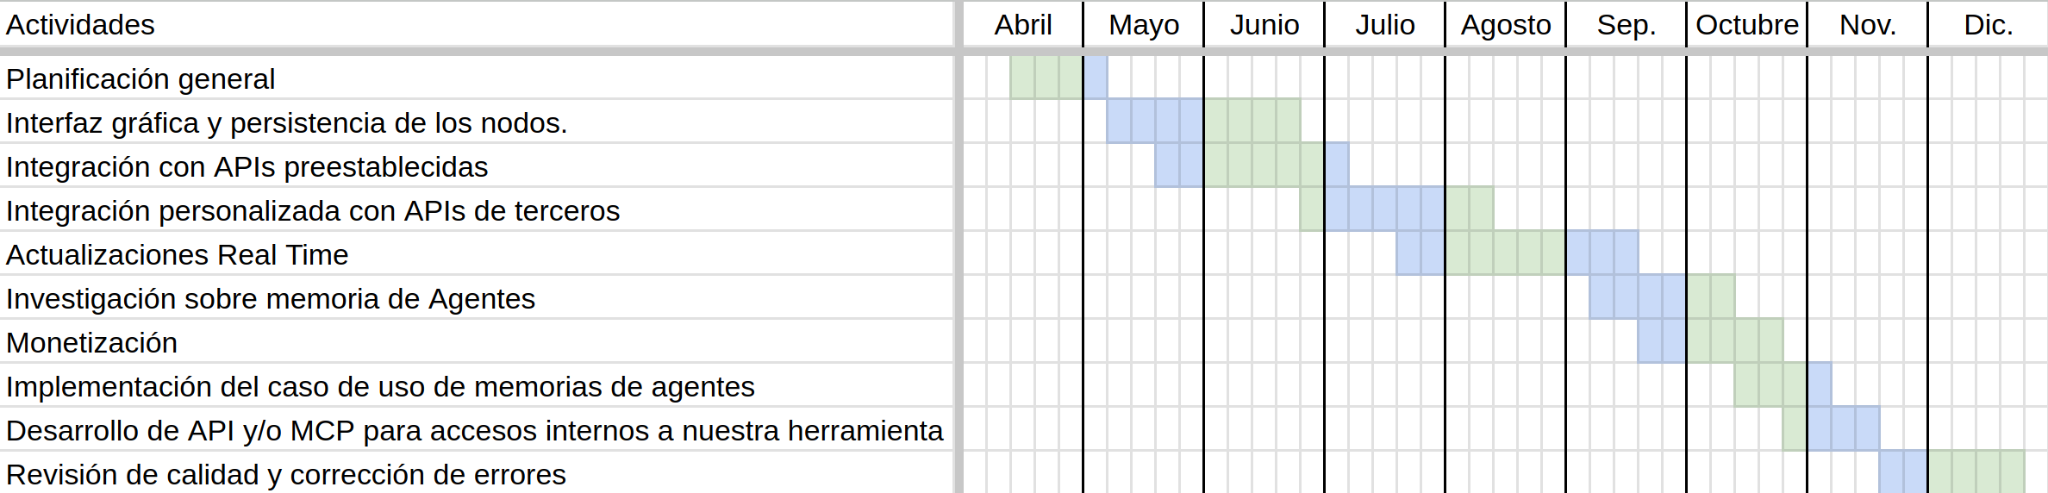
\includegraphics[width=\textwidth]{figuras/fig01.png}
  \caption{Cronograma del proyecto}
  \label{fig:cronograma_inicial}
\end{figure}

\section{Ejecución real del proyecto}
El trabajo se desarrolló de forma ordenada y estructurada, siguiendo el diagrama de Gantt presentado en la sección anterior. Sin embargo, se produjo un desvío con la organización original, dado que se decidió postergar la implementación del sistema de monetización hasta luego de integrar el servicio de MCPs en el producto.

La Figura~\ref{fig:cronograma_actualizado} presenta el cronograma actualizado, en el cual la fase de monetización se desplaza al final del proyecto, luego del desarrollo de la API y del servidor MCP, y se incorporan las actualizaciones en tiempo real y una etapa final de revisión de calidad y corrección de errores.

\begin{figure}[H]
  \centering
  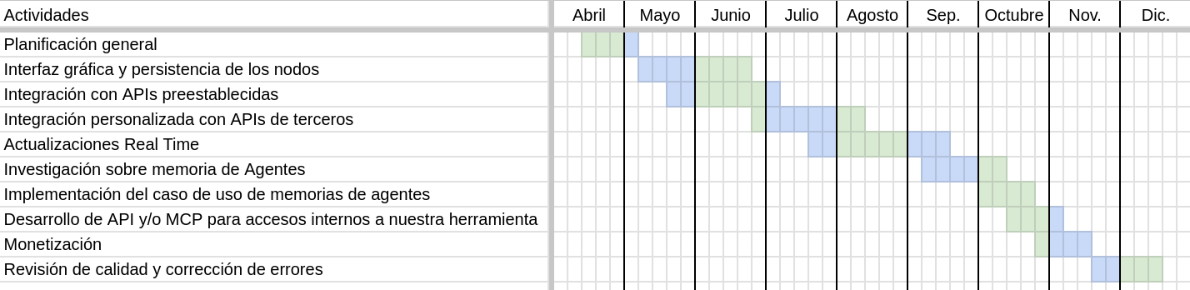
\includegraphics[width=\textwidth]{figuras/fig02.png}
  \caption{Cronograma del proyecto actualizado}
  \label{fig:cronograma_actualizado}
\end{figure}

Las tareas se distribuyeron entre los integrantes del equipo de forma equitativa, estableciendo objetivos bimensuales y reuniones semanales de avances. Esta organización le dio al equipo gran flexibilidad de desarrollo y autogestión, permitiendo a cada uno enfocarse en la tarea a mano.

\section{Gestión de riesgos}
Durante la planificación se identificaron los principales riesgos que podían afectar el desarrollo y el funcionamiento del sistema. La Tabla~\ref{tab:riesgos} resume cada uno de ellos junto con el tratamiento adoptado, que en la mayoría de los casos se incorporó al propio diseño de la solución.

\begin{table}[H]
  \centering
  \renewcommand{\arraystretch}{1.25}
  \begin{tabularx}{\textwidth}{>{\bfseries}p{0.35\textwidth} X}
    \toprule
    Riesgo & Tratamiento \\
    \midrule
    Cambios o caída de las APIs de terceros & Cada tarjeta muestra su error sin afectar al resto del tablero, y las integraciones del catálogo pueden corregirse desde la aplicación sin desplegar una nueva versión. \\
    Límites de uso de las APIs externas & El resultado de cada tarjeta se guarda en caché durante el tiempo configurado, de modo que cada API se consulta como máximo una vez por período. \\
    Filtración de credenciales de los usuarios & Los valores se cifran con AES-GCM por ámbito, nunca se devuelven por la API y las peticiones salientes se realizan con un cliente HTTP que bloquea direcciones internas. \\
    Límites de los planes gratuitos de Vercel, MongoDB Atlas y Redis Cloud & El sistema puede desplegarse también con Docker, y la migración a AWS se planifica al superar los 500.000 usuarios y se ejecuta antes de alcanzar 1.000.000 (Capítulo~\ref{chap:monetizacion}). \\
    Disponibilidad del equipo & El trabajo se organizó en iteraciones de dos semanas, con una replanificación al cierre de cada una. \\
    Cambios en el protocolo MCP, de reciente aparición & El servidor MCP se mantiene separado del backend y consume su API REST, por lo que puede actualizarse de forma independiente. \\
    \bottomrule
  \end{tabularx}
  \caption{Riesgos del proyecto y su tratamiento}
  \label{tab:riesgos}
\end{table}
% !TEX root = ../main.tex
\chapter{Requerimientos del Proyecto}

\section{Descripción general de la aplicación}
El sistema es una aplicación web de tableros inteligentes que permite a los usuarios organizar información proveniente de múltiples fuentes en un único espacio visual, flexible y personalizable. Su unidad básica es la tarjeta, un componente visual que puede contener tanto información estática ingresada por el usuario como datos dinámicos obtenidos en tiempo real desde APIs externas u otras fuentes configurables.

Las tarjetas se disponen libremente sobre un tablero de estilo lienzo, donde el usuario puede posicionarlas, redimensionarlas y conectarlas entre sí mediante hilos visuales que expresan relaciones, dependencias o secuencias temporales. Esta metáfora, inspirada en el clásico pizarrón de corcho, permite construir estructuras de información que se adaptan naturalmente a casos de uso muy diversos.

El sistema ofrece un conjunto de integraciones predefinidas con servicios populares, que permiten a cualquier usuario conectar tarjetas a fuentes de datos conocidas con mínima configuración. Para usuarios más avanzados, se habilita la posibilidad de conectar tarjetas a APIs externas personalizadas o a servidores MCP, extendiendo las capacidades del sistema de forma prácticamente ilimitada.

Adicionalmente, el sistema incorpora un mecanismo de memorias, que permite al usuario guardar y organizar información persistente dentro del tablero, vinculándola con otras tarjetas para mantener contexto a lo largo del tiempo. Esta funcionalidad resulta especialmente útil en flujos de trabajo que involucran modelos de lenguaje u otros sistemas que se benefician del contexto acumulado.

El acceso a la plataforma requiere autenticación, pudiendo el usuario registrarse con email y contraseña, o mediante proveedores externos como Google o GitHub. Cada usuario gestiona sus propios tableros de forma privada, con la posibilidad de compartirlos o exportarlos según sus necesidades.

\section{Usuarios representativos}
Los usuarios a quienes el proyecto está dirigido cumplen con la siguiente descripción, y a partir de esta se toman decisiones de diseño que mejor reflejen las necesidades de las mismas:

\begin{itemize}
  \item \textbf{Edad:} Personas de 16 años en adelante, dado que la herramienta está orientada a la gestión y organización de información, considerando la adolescencia como el punto en que una persona pasa a autogestionar sus tareas. Se estima que la mayor concentración de usuarios se ubica en el rango de edades entre los 20 y 45 años, apuntando al público en edad productiva, siendo quienes más información gestionan en el día a día. A modo de no excluir a los grupos mayores o con dificultades para manejar la tecnología, se diseñó una interfaz sencilla y amigable, con herramientas o templates de casos de usos típicos ya armados para reducir la fricción inicial.
  \item \textbf{Lenguaje:} Se espera que la aplicación pueda introducirse exitosamente en una franja amplia del mercado, por lo que está destinada a personas hispanohablantes y angloparlantes en la primera fase del desarrollo.
  \item \textbf{Usos y costumbres:} Son personas que buscan simplificar las rutinas de su vida diaria, quieran mejorar la organización de sus actividades, o que manejan grandes volúmenes de información con actualizaciones constantes. También se supone que la mayoría de los usuarios son nativos digitales, aquellos que optan por una gestión complementada con tecnología sobre los medios tradicionales.
  \item \textbf{Características no influyentes:} No se encontraron razones para discriminar a los usuarios por nivel socioeconómico, sexo, nacionalidad, oficio y cultura.
\end{itemize}

\section{Especificación de Requisitos (MVP)}

\subsection{Listado de Requisitos Funcionales}
A continuación se detallan en una tabla todos los requisitos funcionales iniciales.

\begin{table}[H]
  \centering
  \renewcommand{\arraystretch}{1.2}
  \begin{tabularx}{\textwidth}{>{\bfseries}l X l}
    \toprule
    ID & Requisito & Prioridad \\
    \midrule
    RF-01 & El usuario puede registrarse en la plataforma & Alta \\
    RF-02 & El usuario puede iniciar sesión con un proveedor externo (Google, GitHub) & Media \\
    RF-03 & El usuario puede cerrar sesión & Alta \\
    RF-04 & El usuario puede crear un tablero personalizado & Alta \\
    RF-05 & El usuario puede agregar tarjetas al tablero & Alta \\
    RF-06 & El usuario puede vincular tarjetas entre sí mediante hilos visuales & Alta \\
    RF-07 & El usuario puede conectar una tarjeta a una API externa predefinida & Alta \\
    RF-08 & El usuario puede conectar una tarjeta a una API externa personalizada & Media \\
    RF-09 & Las tarjetas se actualizan automáticamente con los últimos datos de su fuente & Alta \\
    RF-10 & El usuario puede conectarse a un tablero mediante un servidor MCP & Media \\
    RF-11 & El usuario puede organizar y etiquetar memorias dentro del tablero & Media \\
    RF-12 & El usuario puede personalizar el estilo visual de cada tarjeta & Baja \\
    RF-13 & El usuario puede compartir o exportar un tablero & Baja \\
    \bottomrule
  \end{tabularx}
  \caption{Listado de Requisitos Funcionales Iniciales}
  \label{tab:rf_iniciales}
\end{table}

\subsection{Listado de Requisitos no funcionales}
El trabajo apunta a tener un alto grado de calidad, propio de un proyecto de ingeniería informática. Para ello, se busca cumplir no solo con los requisitos funcionales propuestos del producto, sino también requisitos no propios del negocio, que refieren a la calidad del servicio en sí.

A continuación se detalla el listado de requisitos no funcionales de la aplicación:

\begin{table}[H]
  \centering
  \renewcommand{\arraystretch}{1.2}
  \begin{tabularx}{\textwidth}{>{\bfseries}l X l}
    \toprule
    ID & Requisito & Categoría \\
    \midrule
    RNF-01 & Los tableros deben actualizarse en menos de 5 segundos ante cambios en las tarjetas & Performance \\
    RNF-02 & Las credenciales de APIs externas deben almacenarse de forma segura & Seguridad \\
    RNF-03 & El sistema debe ser usable sin conocimientos técnicos avanzados para APIs predefinidas & Usabilidad \\
    RNF-04 & El sistema debe soportar la incorporación de nuevas integraciones sin rediseño estructural & Extensibilidad \\
    RNF-05 & El tablero debe ser responsivo y funcionar correctamente en navegadores modernos & Compatibilidad \\
    RNF-06 & La comunicación con servidores MCP debe seguir el protocolo estándar definido & Interoperabilidad \\
    RNF-07 & La aplicación debe ofrecer sus servicios con un 99.9\% de disponibilidad & Disponibilidad \\
    \bottomrule
  \end{tabularx}
  \caption{Listado de Requisitos No Funcionales Iniciales}
  \label{tab:rnf_iniciales}
\end{table}

\subsection{Historias de usuario}

\subsubsection*{RF-01 - Registrarse en la plataforma}
Como usuario nuevo, quiero poder registrarme con email y contraseña, para acceder a la plataforma con una cuenta propia.

\textbf{Criterios de aceptación:}
\begin{itemize}
  \item El formulario requiere nombre, email y contraseña
  \item Se valida que el email tenga formato válido y no esté ya registrado
  \item La contraseña debe cumplir requisitos mínimos de seguridad (mínimo 8 caracteres)
  \item Al registrarse exitosamente, el usuario queda autenticado y es redirigido al tablero
\end{itemize}

\subsubsection*{RF-02 - Iniciar sesión con proveedor externo}
Como usuario, quiero poder iniciar sesión con Google o GitHub, para acceder a la plataforma sin tener que crear credenciales nuevas.

\textbf{Criterios de aceptación:}
\begin{itemize}
  \item Se muestran botones de acceso rápido con Google y GitHub
  \item Al autenticarse por primera vez con un proveedor externo, se crea una cuenta automáticamente
  \item Si ya existe una cuenta con el mismo email, se vincula al proveedor
\end{itemize}

\subsubsection*{RF-03 - Cerrar sesión}
Como usuario autenticado, quiero poder cerrar sesión, para proteger mi cuenta al usar dispositivos compartidos.

\textbf{Criterios de aceptación:}
\begin{itemize}
  \item Hay una opción visible de cierre de sesión en la interfaz
  \item Al cerrar sesión, el usuario es redirigido a la pantalla de login
  \item Tras cerrar sesión, no es posible acceder a rutas protegidas sin autenticarse nuevamente
\end{itemize}

\subsubsection*{RF-04 - Crear un tablero}
Como usuario, quiero poder crear un tablero personalizado, para tener un espacio de trabajo dedicado a un tema o proyecto.

\textbf{Criterios de aceptación:}
\begin{itemize}
  \item El usuario puede crear un tablero asignándole un nombre
  \item El tablero aparece en el listado de tableros del usuario
  \item El tablero recién creado se abre vacío y listo para agregar tarjetas
\end{itemize}

\subsubsection*{RF-05 - Agregar tarjeta al tablero}
Como usuario, quiero poder agregar una tarjeta al tablero, para organizar una nueva pieza de información en mi espacio de trabajo.

\textbf{Criterios de aceptación:}
\begin{itemize}
  \item La tarjeta se crea con un título editable
  \item Puede posicionarse libremente en el tablero
  \item Puede configurarse como estática o conectada a una fuente
  \item Puede establecer una conexión con una API
\end{itemize}

\subsubsection*{RF-06 - Vincular tarjetas mediante hilos visuales}
Como usuario, quiero poder conectar dos tarjetas con un hilo visual, para expresar relaciones, dependencias o secuencias entre ellas.

\textbf{Criterios de aceptación:}
\begin{itemize}
  \item El usuario puede iniciar un hilo desde el borde de una tarjeta y conectarlo a otra
  \item El hilo persiste al recargar el tablero
  \item El usuario puede eliminar un hilo sin afectar las tarjetas
  \item Se puede conectar una tarjeta a múltiples tarjetas simultáneamente
  \item El usuario puede agregar una etiqueta al hilo para describir la relación
  \item El usuario puede indicar la dirección de la relación mediante flechas en uno o ambos extremos
  \item El usuario puede elegir el grosor del hilo y su color dentro de una paleta predefinida
  \item Solo los editores del tablero pueden modificar el estilo de un hilo
\end{itemize}

\subsubsection*{RF-07 - Conectar una tarjeta a una API predefinida}
Como usuario, quiero poder conectar una tarjeta a una integración predefinida (por ejemplo: precio de un vuelo, estado de un repositorio), para ver datos actualizados sin necesidad de configurar nada técnico.

\textbf{Criterios de aceptación:}
\begin{itemize}
  \item Hay un listado de integraciones predefinidas disponibles para seleccionar
  \item El usuario completa únicamente los parámetros visibles de la integración (ej: ciudad de origen, nombre del repositorio)
  \item La tarjeta muestra los datos obtenidos de la API
  \item Se indica visualmente cuándo fue la última actualización
\end{itemize}

\subsubsection*{RF-08 - Conectar una tarjeta a una API personalizada}
Como usuario avanzado, quiero poder conectar una tarjeta a una API externa propia, para traer cualquier dato que necesite aunque no esté entre las integraciones predefinidas.

\textbf{Criterios de aceptación:}
\begin{itemize}
  \item El usuario puede ingresar la URL del endpoint, método HTTP y headers necesarios
  \item Las credenciales se almacenan de forma segura y no se exponen en la interfaz
  \item La tarjeta muestra la respuesta de la API o un mensaje de error descriptivo si la llamada falla
  \item El usuario puede editar o eliminar la configuración de la API en cualquier momento
\end{itemize}

\subsubsection*{RF-09 - Actualización automática de datos}
Como usuario, quiero que las tarjetas conectadas a fuentes externas se actualicen automáticamente, para que el tablero refleje siempre el estado actual de la información.

\textbf{Criterios de aceptación:}
\begin{itemize}
  \item Las tarjetas conectadas se actualizan periódicamente sin intervención del usuario
  \item El intervalo de actualización es configurable por tarjeta
  \item Si una actualización falla, la tarjeta muestra el último dato disponible junto con un indicador de error
  \item La actualización no interrumpe la interacción del usuario con el tablero
\end{itemize}

\subsubsection*{RF-10 - Conectarse a un tablero mediante un servidor MCP}
Como usuario avanzado, quiero poder conectarme a un tablero mediante MCP, para integrar contexto y datos provenientes de modelos de lenguaje u otros sistemas compatibles.

\textbf{Criterios de aceptación:}
\begin{itemize}
  \item El usuario puede ingresar la URL del servidor MCP y los parámetros necesarios
  \item El tablero permite acciones por parte de agentes
  \item La conexión sigue el protocolo MCP estándar
  \item Se indica claramente si el servidor no responde o devuelve un error
\end{itemize}

\subsubsection*{RF-11 - Organizar y etiquetar memorias}
Como usuario, quiero poder guardar fragmentos de información como memorias dentro del tablero y etiquetarlas, para mantener el contexto acumulado a lo largo del tiempo.

\textbf{Criterios de aceptación:}
\begin{itemize}
  \item El usuario puede crear una tarjeta de tipo memoria con texto libre
  \item Las memorias pueden etiquetarse con categorías personalizadas
  \item Las memorias pueden vincularse con otras tarjetas del tablero mediante hilos
  \item Las memorias persisten entre sesiones
\end{itemize}

\subsubsection*{RF-12 - Personalizar el estilo visual de una tarjeta}
Como usuario, quiero poder cambiar el color, tamaño o apariencia de una tarjeta, para diferenciar visualmente la información según su relevancia o tipo.

\textbf{Criterios de aceptación:}
\begin{itemize}
  \item El usuario puede elegir entre una paleta de colores para el fondo de la tarjeta
  \item El usuario puede cambiar el tamaño de la tarjeta redimensionándola libremente
  \item Los cambios de estilo persisten al recargar el tablero
  \item El usuario puede elegir el color blanco, y el texto de la tarjeta adopta automáticamente un color legible sobre el fondo elegido
  \item El usuario puede agregar un borde continuo, de guiones o de puntos, y elegir su grosor y su color
  \item El usuario puede volver a ajustar la tarjeta al tamaño de su contenido
  \item El usuario puede alinear el texto de la tarjeta horizontalmente (a la izquierda, al centro o a la derecha) y verticalmente (arriba, en el medio o abajo)
  \item Solo los editores del tablero pueden modificar el estilo de una tarjeta
\end{itemize}

\subsubsection*{RF-13 - Compartir o exportar un tablero}
Como usuario, quiero poder compartir mi tablero con otros o exportarlo, para colaborar o guardar una copia de mi trabajo.

\textbf{Criterios de aceptación:}
\begin{itemize}
  \item El usuario puede generar un enlace de solo lectura para compartir el tablero
  \item El usuario puede exportar el tablero en al menos un formato estándar (por ejemplo, JSON o imagen)
  \item El enlace compartido muestra el estado actual del tablero al momento de la visita
\end{itemize}
% !TEX root = ../main.tex
\chapter{Documentación de Interfaces (MVP)}

\section{Diagrama de navegación / flujo de pantallas}
La Figura~\ref{fig:diagrama_navegacion} muestra el diagrama de navegación de la aplicación, en el cual los rectángulos corresponden a las pantallas, los círculos a las acciones que el usuario realiza sobre ellas y las flechas al recorrido entre unas y otras. A partir de la lista de tableros el usuario accede a un tablero, donde agrega, edita, une, recarga y elimina tarjetas, y comparte el tablero configurando sus accesos.

\begin{figure}[H]
  \centering
  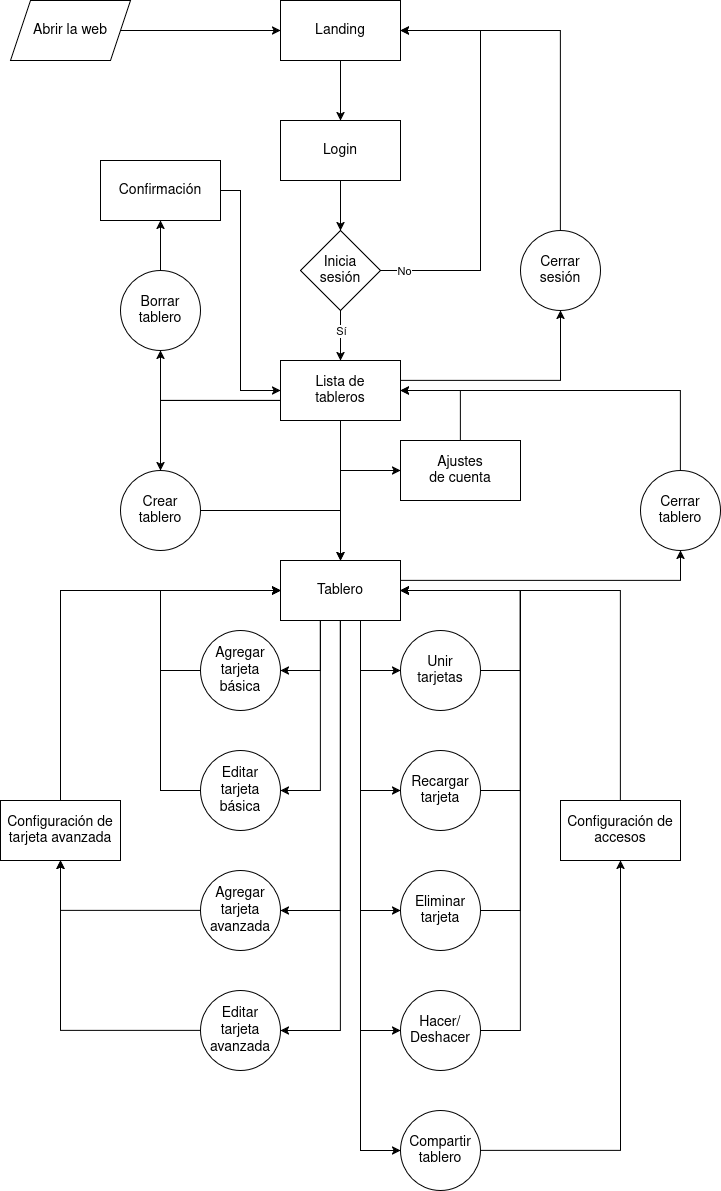
\includegraphics[width=0.82\textwidth]{figuras/fig03.png}
  \caption{Diagrama de Navegación}
  \label{fig:diagrama_navegacion}
\end{figure}
% !TEX root = ../main.tex
\chapter{Diseño de Alto Nivel}

\section{Arquitectura general del sistema}
El sistema sigue una arquitectura cliente-servidor, y está particionado en 4 componentes lógicos propietarios y 5 servicios: Un frontend desarrollado en SvelteKit \cite{sveltekit_docs}, un backend en GoLang \cite{go_docs}, un módulo de actualizaciones realtime en NodeJS \cite{nodejs_docs}, un servidor MCP con xMCP \cite{xmcp_docs} en NodeJS, una base de datos no relacional de documentos, una base de datos key-value, un servidor STUN, un proveedor de mailing y un proveedor de pagos.

El frontend es una SPA que renderiza el tablero tipo lienzo y consume la API REST del backend. El backend, estructurado con una arquitectura hexagonal, orquesta la persistencia en MongoDB, el caché en Redis y la ejecución de integraciones contra fuentes externas a través del motor Executer.

La Figura~\ref{fig:diagrama_contexto} corresponde al diagrama de contexto del sistema, en el cual se identifican los actores que interactúan con él y los servicios externos de los que depende. El usuario accede desde el navegador por HTTPS y WebSocket, mientras que un agente de IA lo hace a través del protocolo MCP, autenticado con un token personal del usuario. Hacia afuera, el sistema consulta las APIs de terceros que configura cada tarjeta, utiliza Google para el inicio de sesión y los consentimientos OAuth2 \cite{rfc6749}, y Resend \cite{resend_docs} para el envío de correos. Los cursores de los participantes de un tablero viajan directamente entre navegadores mediante WebRTC, con el servidor de señalización de PeerJS \cite{peerjs_docs} como intermediario para establecer la conexión. Por último, el sistema cobra las suscripciones de los planes pagos a través de Mercado Pago \cite{mercadopago_docs}.

\begin{figure}[H]
  \centering
  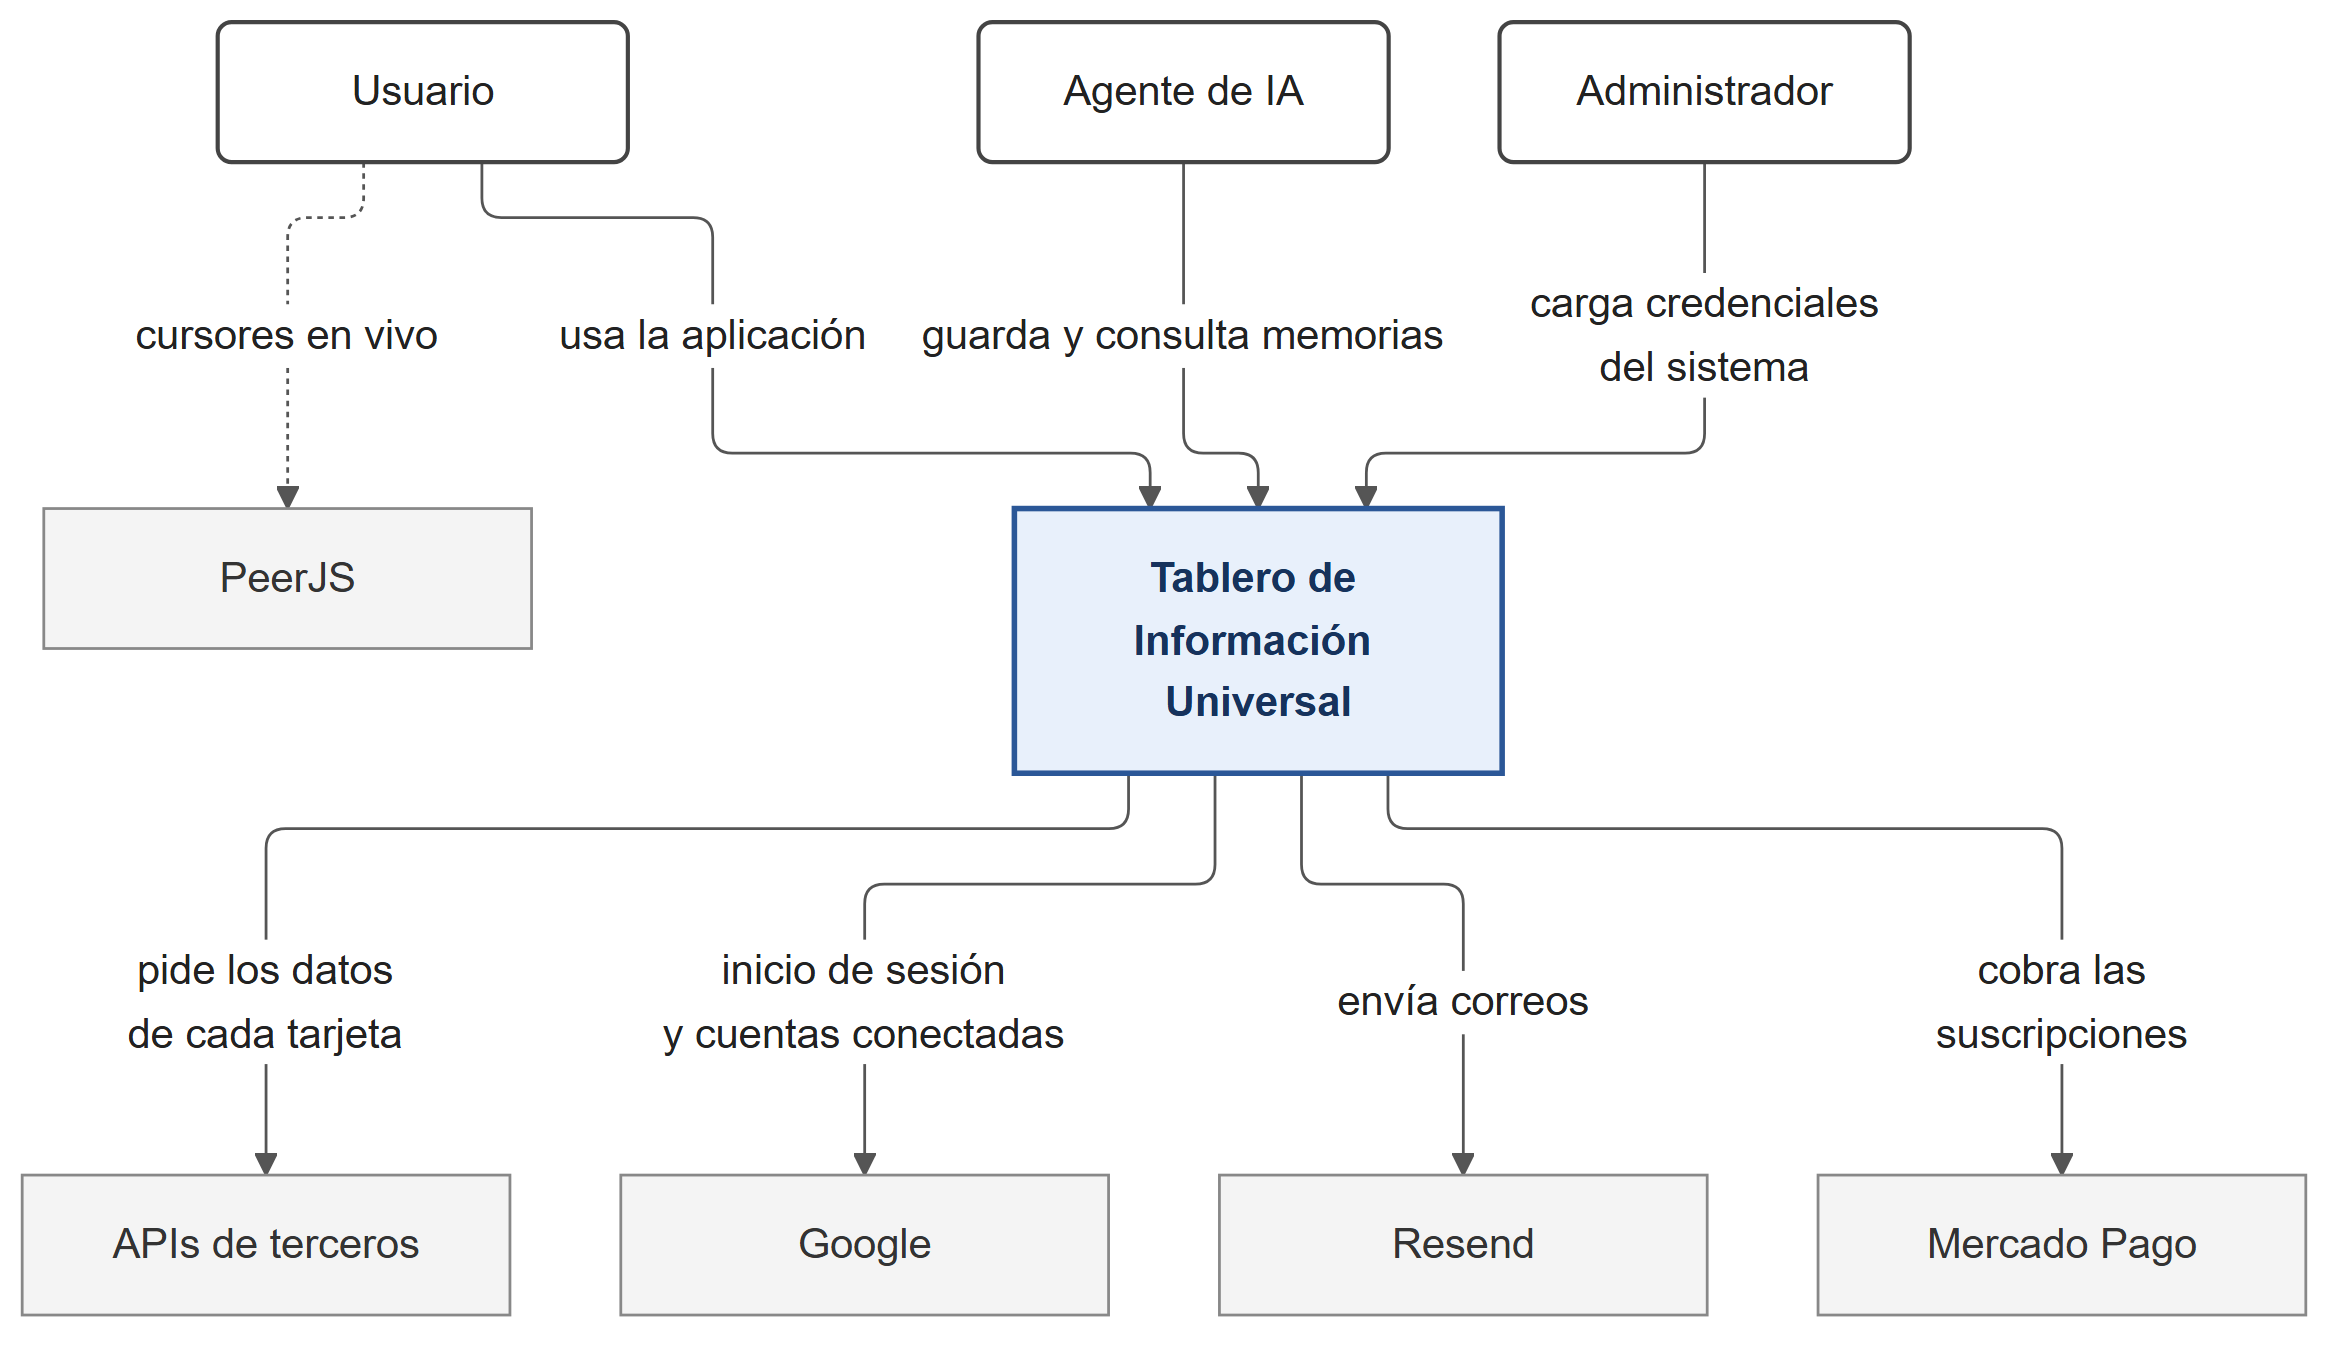
\includegraphics[width=0.92\textwidth]{figuras/fig04.png}
  \caption{Diagrama de contexto}
  \label{fig:diagrama_contexto}
\end{figure}

En la Figura~\ref{fig:diagrama_servicios} se representa el diagrama de servicios, en el cual se detallan los componentes que conforman el sistema y la forma en la que se comunican. Todos los servicios se publican detrás de un único origen, y un proxy inverso distribuye cada pedido según el prefijo de su ruta: \texttt{/api} al backend, \texttt{/ws} al servicio de tiempo real, \texttt{/mcp} al servidor MCP y el resto al frontend. El backend es el único servicio que escribe los datos de negocio en MongoDB, utiliza Redis como caché de resultados, almacén de sesiones y registro de límites de frecuencia de solicitudes, y con Mercado Pago crea y modifica las suscripciones a través de su API y maneja webhooks. El servicio de tiempo real no modifica datos: recibe los cambios de la colección de tableros mediante un change stream de MongoDB y consulta al backend el rol de cada usuario que se conecta. De la misma forma, el servidor MCP no accede a las bases de datos, sino que reenvía al backend cada operación del agente con el token del usuario, por lo que se aplican las mismas reglas de autorización que en la aplicación web.

\begin{figure}[H]
  \centering
  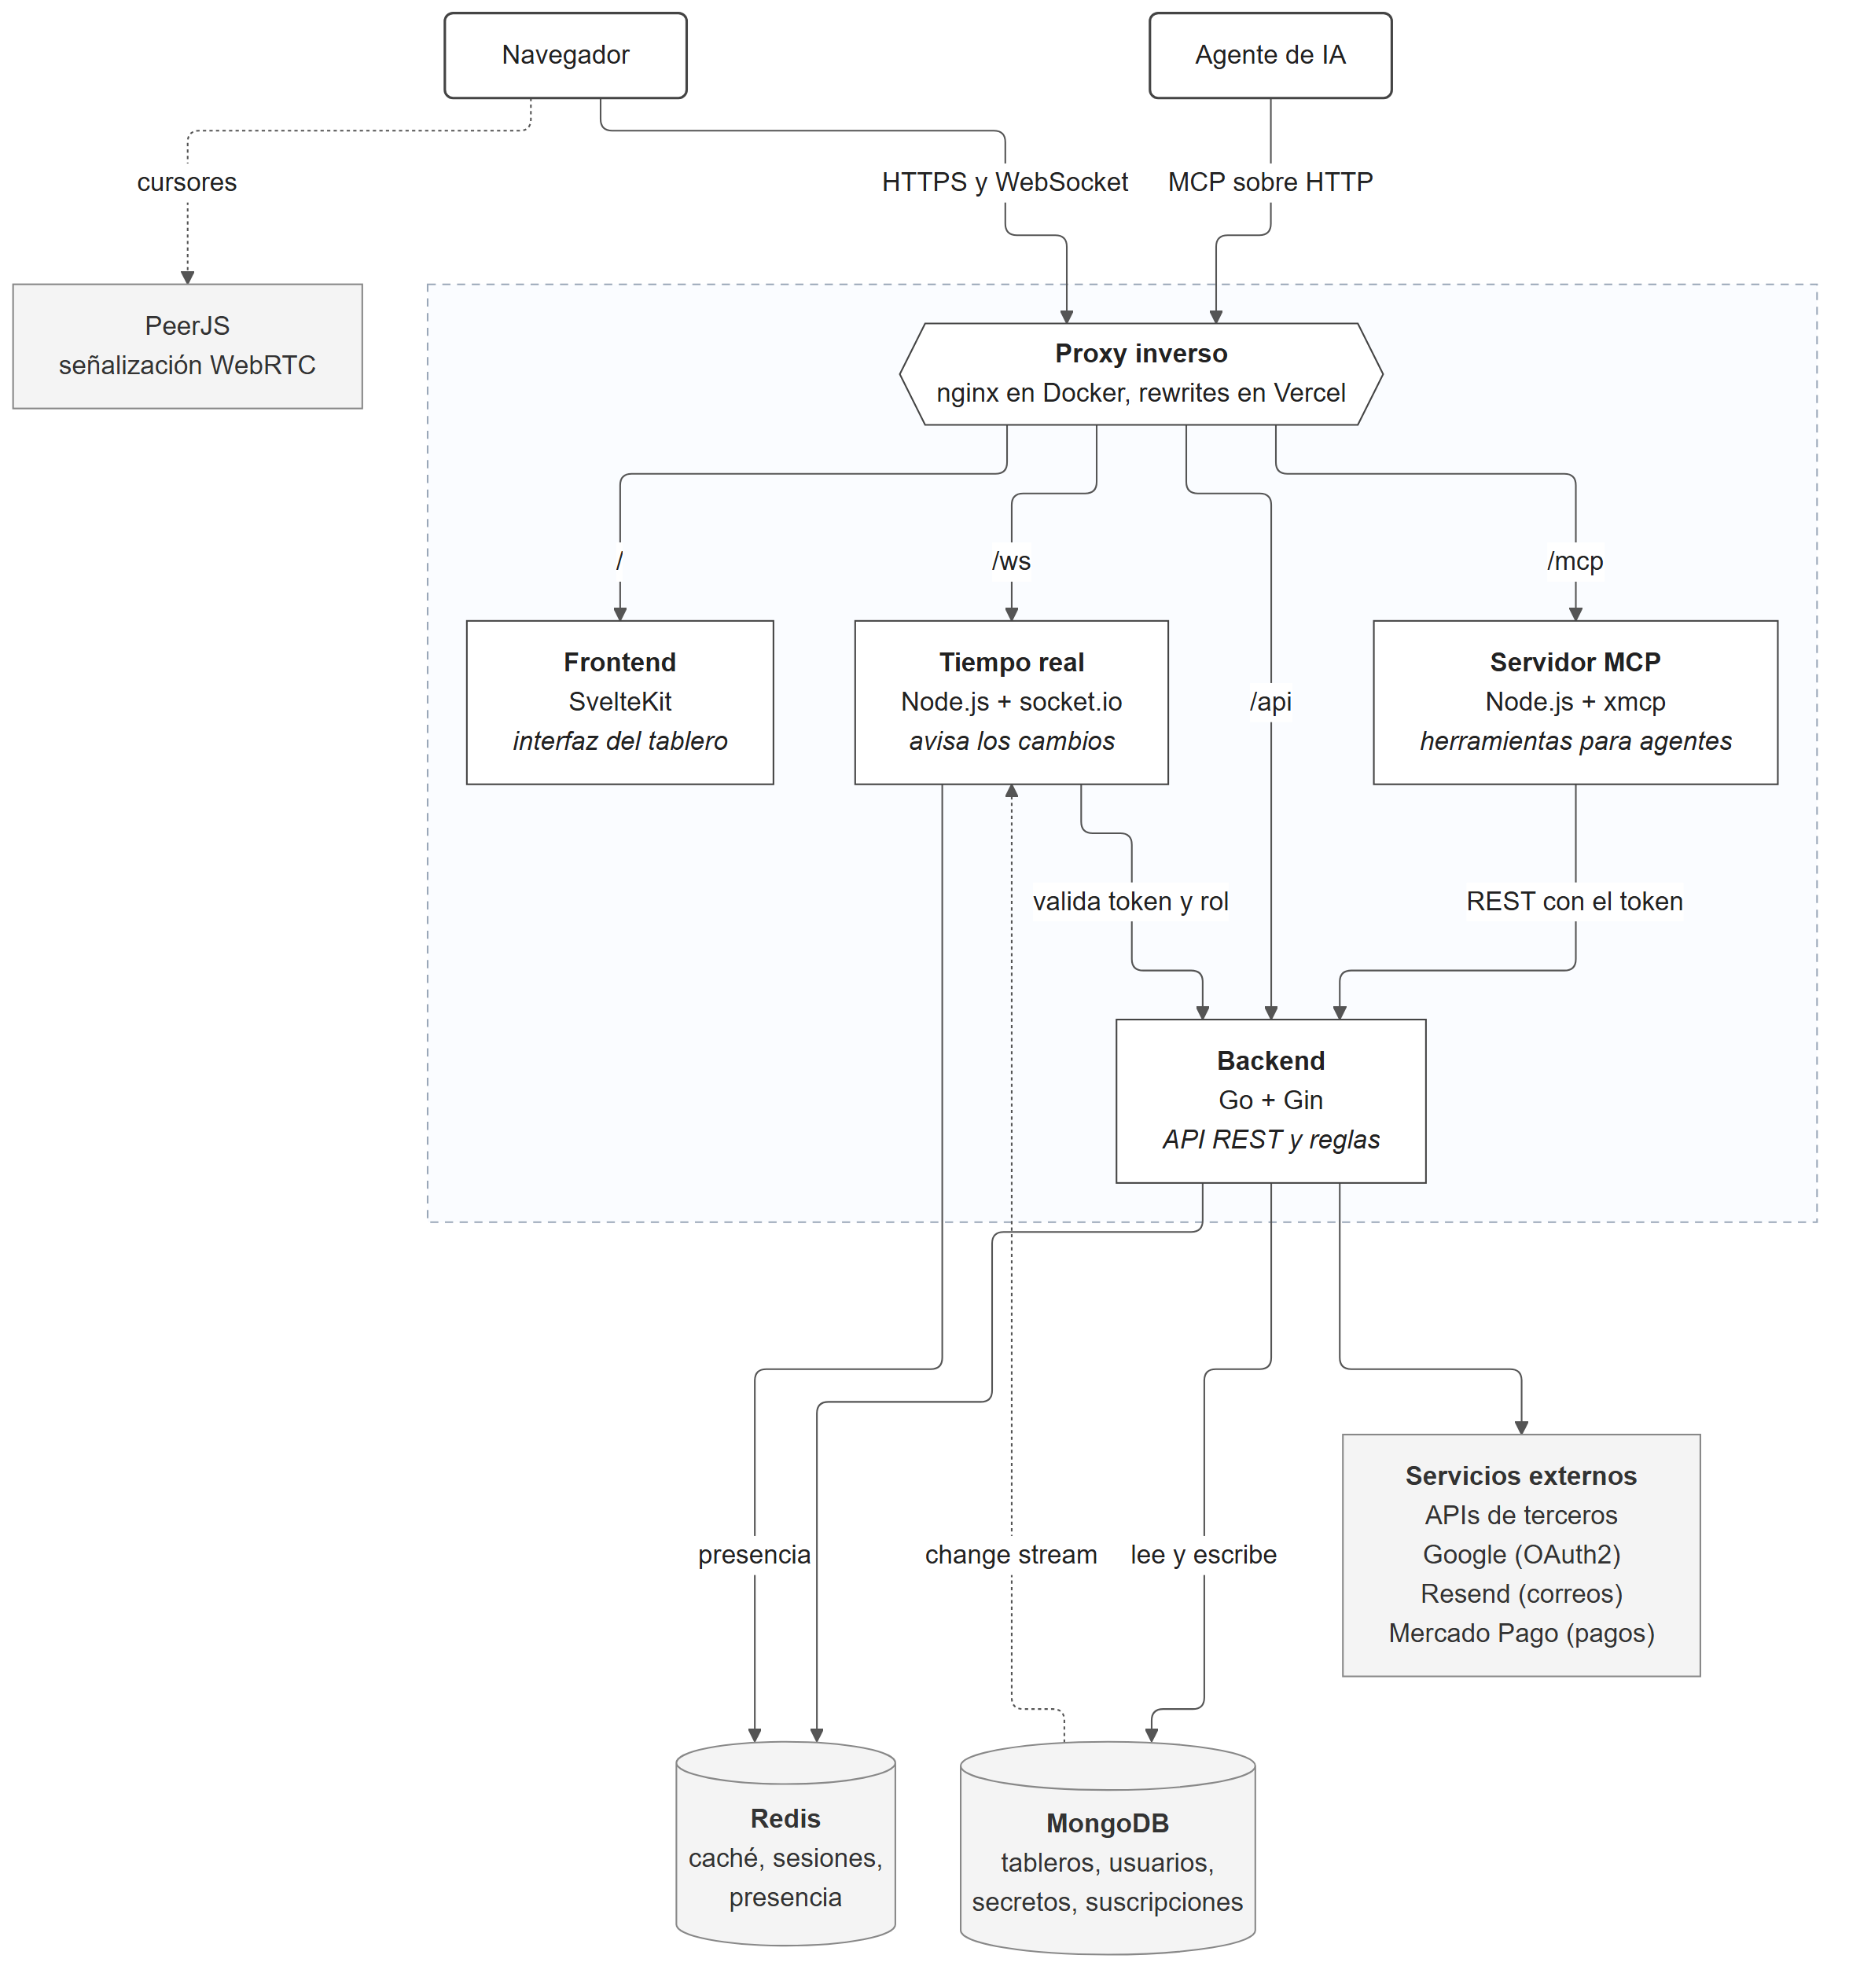
\includegraphics[width=0.92\textwidth]{figuras/fig05.png}
  \caption{Diagrama de servicios}
  \label{fig:diagrama_servicios}
\end{figure}

Para la primera fase de desarrollo del producto, el sistema se despliega en Vercel \cite{vercel_docs}, el cual provee el hosting de la web, las funciones serverless de Go y Node, y el dominio. Para las bases de datos, se utilizan los servicios de MongoDB Atlas \cite{mongodb_docs} y Redis Cloud \cite{redis_docs} respectivamente. El servicio STUN está provisto por PeerJS, el envío de mensajes está gestionado por Resend, y los pagos se procesan con Mercado Pago.

La Figura~\ref{fig:arq_vercel} representa el despliegue en Vercel, en el cual cada carpeta del repositorio se publica como un servicio del mismo proyecto: el frontend con el adaptador de SvelteKit para Vercel, el backend como función de Go, y los servicios de tiempo real y MCP como funciones de Node.js. Las reglas de reescritura del archivo \texttt{vercel.json} cumplen la funcion del proxy inverso, dirigiendo \texttt{/api}, \texttt{/ws} y \texttt{/mcp} a su respectivo servicio y el resto al frontend. Las líneas punteadas representan la variable \texttt{API\_URL}, mediante la cual Vercel les indica a los servicios de tiempo real y MCP la dirección del backend. Servir todo desde un mismo origen evita configurar CORS, permite que la cookie de sesión se envíe con la política \texttt{SameSite=Strict} y hace que una misma compilación del frontend funcione en cualquier dominio, incluidas las URLs de vista previa.

\begin{figure}[H]
  \centering
  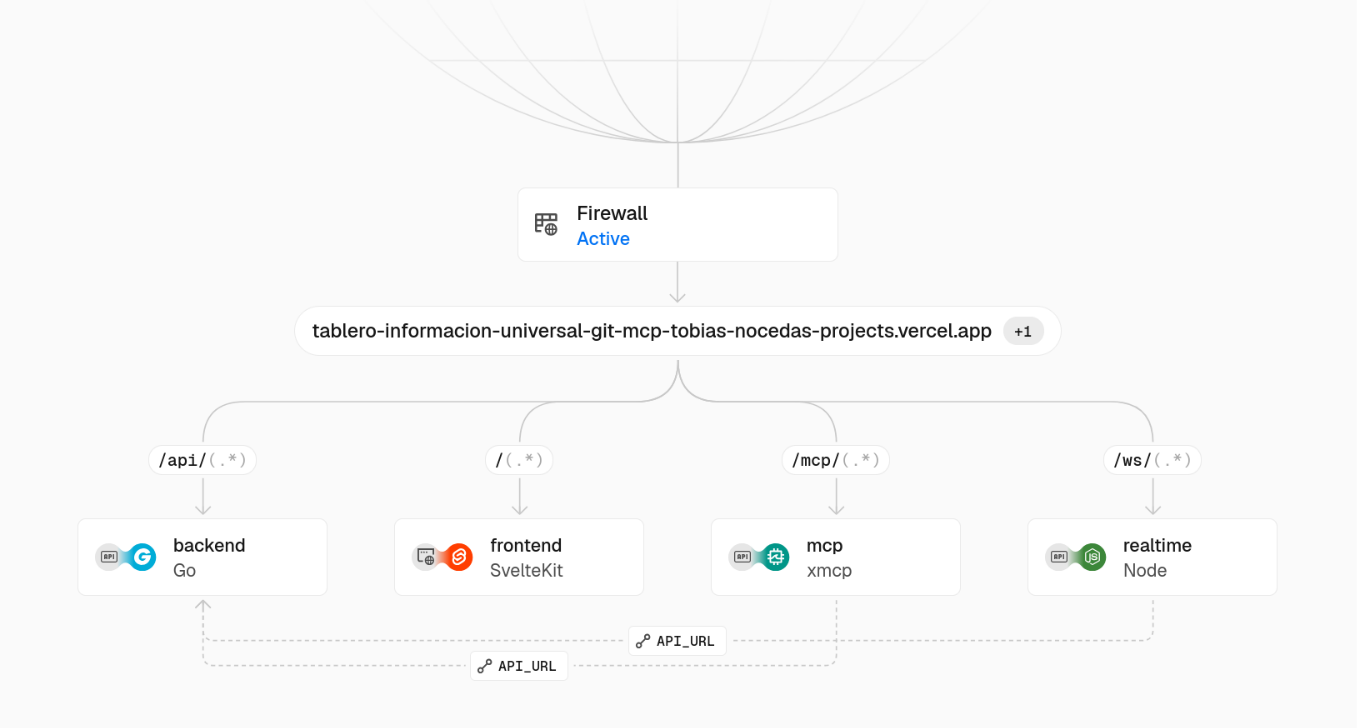
\includegraphics[width=0.95\textwidth]{figuras/fig06.png}
  \caption{Diagrama de arquitectura en Vercel}
  \label{fig:arq_vercel}
\end{figure}

Para el desarrollo local, se utiliza un conjunto de contenedores orquestados con Docker Compose \cite{docker_compose_docs}. Esta separación permite escalar de forma horizontal los componentes que lo requieran (típicamente el backend y el motor de actualización) sin afectar al resto, y simplifica el reemplazo de cualquier pieza individual a medida que el producto evoluciona. La Figura~\ref{fig:arq_docker} representa esta topología de despliegue. El contenedor application load balancer, que ejecuta un servidor Nginx \cite{nginx_docs}, actúa como proxy inverso y cumple la misma función que las reglas de reescritura de Vercel, centralizando el acceso a los distintos servicios. Es el único contenedor que expone un puerto al exterior (80), mientras que MongoDB y Redis permanecen accesibles únicamente desde las redes internas de Docker. MongoDB se configura como un replica set de un único nodo para habilitar el uso de Change Streams.

\begin{figure}[H]
  \centering
  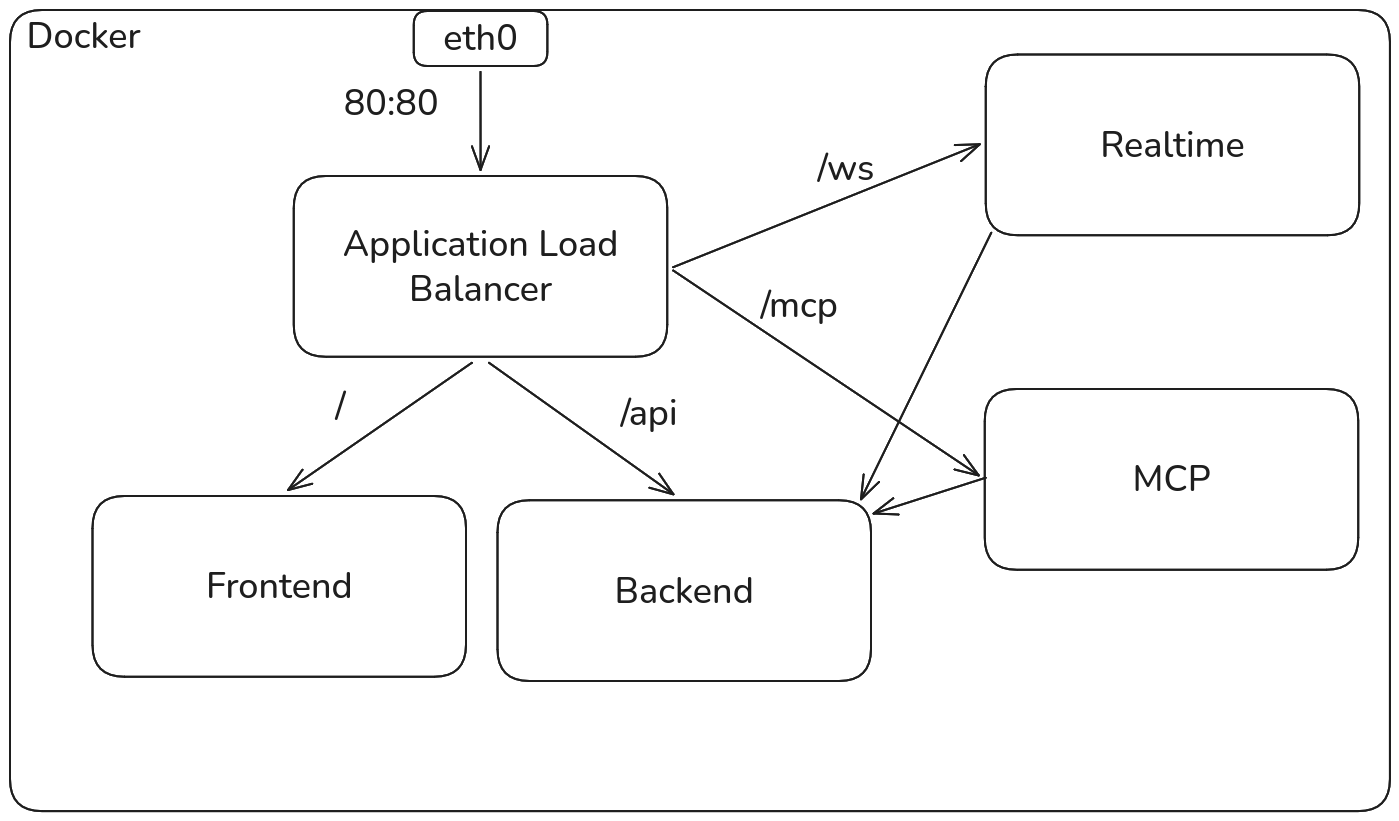
\includegraphics[width=0.9\textwidth]{figuras/fig07.png}
  \caption{Diagrama de arquitectura en Docker}
  \label{fig:arq_docker}
\end{figure}

Como trabajo futuro, se plantea un análisis de costos y del mercado, contemplando el escalamiento del producto a medida que aumenta la adopción del mismo, con el objeto de predecir las necesidades del sistema y los requisitos técnicos de migrar el despliegue según sea rentable.

La Figura~\ref{fig:arq_aws} es una propuesta de arquitectura de despliegue del sistema sobre AWS, que no se encuentra implementada y se plantea como posible evolución del despliegue actual en Vercel. En ella, el tráfico de los usuarios ingresa a través de Route 53 y CloudFront, con Cognito resolviendo la autenticación y WAF la protección perimetral. El frontend estático se sirve desde S3, mientras que la lógica de aplicación se concentra en funciones Lambda que orquestan el acceso a la base de datos, el caché y el motor de integraciones. Esta topología materializa la separación de responsabilidades descrita en la sección anterior y permite escalar de forma independiente cada componente.

\begin{figure}[H]
  \centering
  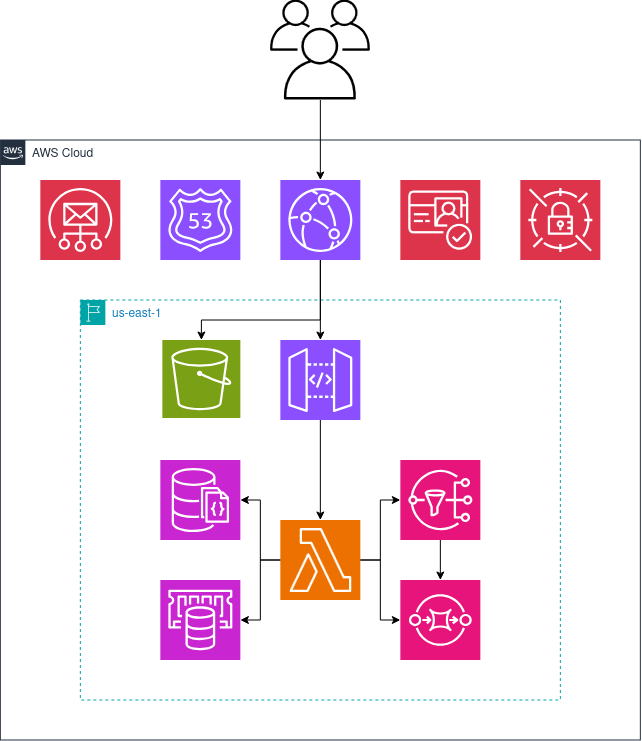
\includegraphics[width=0.82\textwidth]{figuras/fig08.png}
  \caption{Diagrama de arquitectura en AWS}
  \label{fig:arq_aws}
\end{figure}

\section{Flujos de información}
A continuación se describen los principales flujos de información que atraviesan los servicios del sistema, representados mediante diagramas de secuencia.

\subsection{Inicio y la Renovación de Sesión}
La Figura~\ref{fig:seq_sesion} describe el proceso de autenticación y renovación de sesiones. Durante el inicio de sesión, el backend aplica límites de intentos tanto por dirección IP como por cuenta y verifica la contraseña proporcionada mediante Argon2id \cite{rfc9106}. Si la autenticación es exitosa, el backend entrega un token de acceso con una vigencia de 15 minutos y genera un token de refresco, que almacena en Redis y envía al frontend mediante una cookie HttpOnly.

El frontend conserva el token de acceso únicamente en memoria y lo utiliza para autenticar las solicitudes posteriores. Cuando recibe una respuesta HTTP 401, intenta renovar la sesión una única vez, enviando la cookie de refresco al backend. Si la renovación es exitosa, el frontend recibe un nuevo token de acceso y luego reintenta la solicitud original.

En cada renovación, el backend rota el token de refresco y actualiza su registro en Redis. Si detecta que un token de refresco anterior vuelve a utilizarse una vez transcurrido el período de gracia de 10 segundos, revoca toda la familia de sesiones asociada.

\begin{figure}[H]
  \centering
  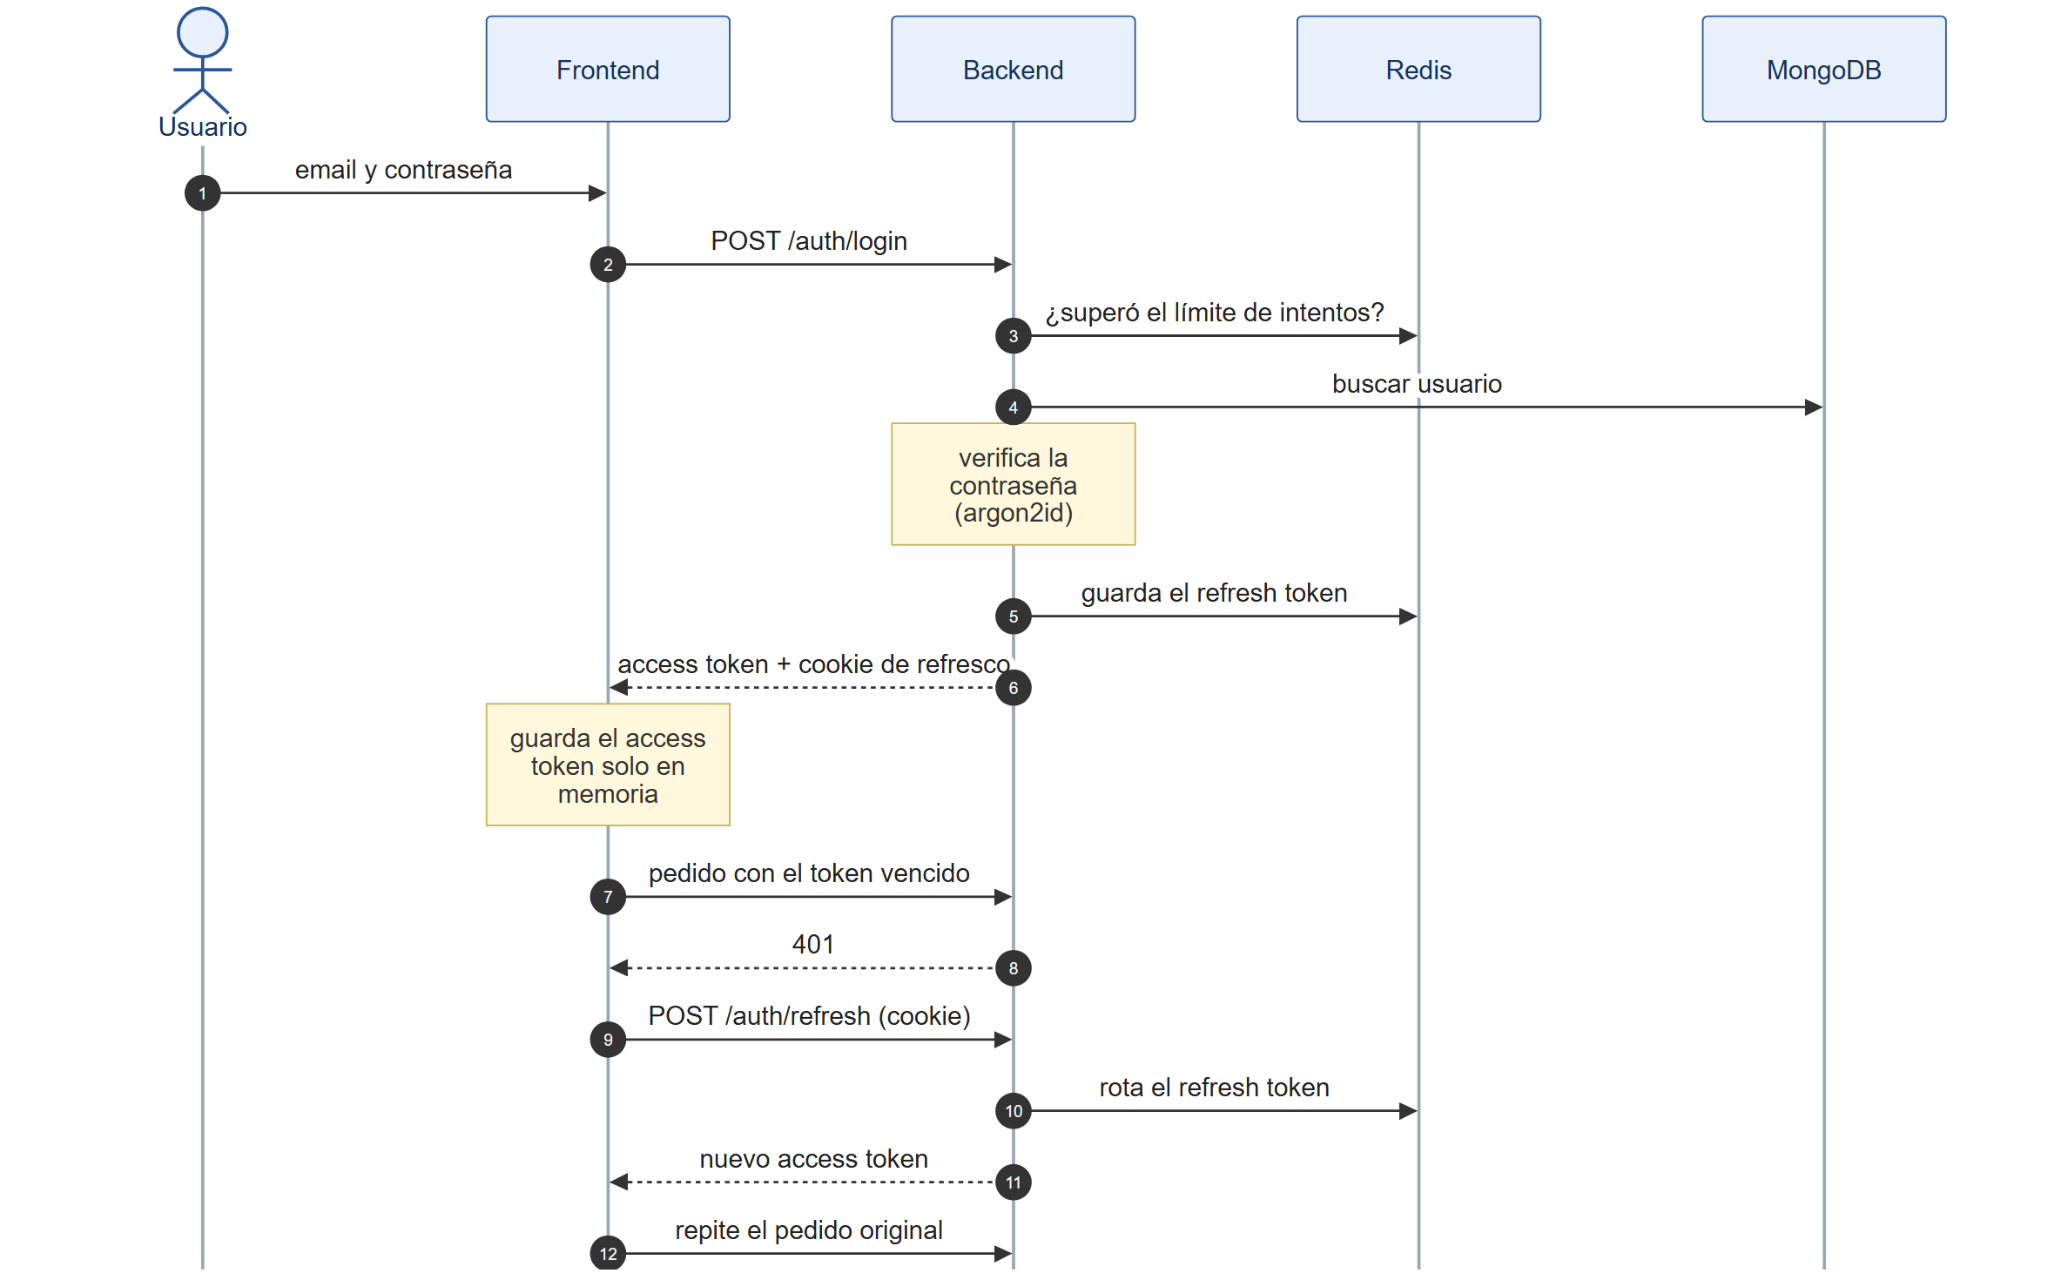
\includegraphics[width=0.95\textwidth]{figuras/fig09.png}
  \caption{Diagrama de secuencia del inicio y la renovación de sesión}
  \label{fig:seq_sesion}
\end{figure}

\subsection{Ejecución de una tarjeta}
La Figura~\ref{fig:seq_ejecucion} ilustra el flujo de ejecución de una tarjeta, uno de los procesos centrales del producto. Ante una solicitud del frontend, el backend verifica que el usuario tenga, como mínimo, el rol de lector sobre el tablero y consulta Redis para determinar si existe un resultado previamente almacenado en caché.

Si no encuentra un resultado, resuelve las credenciales referenciadas por la tarjeta mediante \texttt{\$TOKEN}, utilizando la identidad del usuario indicado en \texttt{RunAs} y verificando que dichas credenciales continúen siendo válidas. Luego, entrega la configuración de la tarjeta al motor de integraciones, que realiza la petición HTTP mediante un cliente que bloquea el acceso a direcciones internas y limita la respuesta a 2 MB y diez segundos. Una vez obtenida la respuesta, el motor la interpreta como JSON o HTML, según el valor del campo \texttt{response}, y aplica la consulta definida en la tarjeta.

Finalmente, el resultado se almacena en Redis durante la cantidad de segundos indicada en \texttt{rate}, con un piso que depende del plan de quien paga el tablero, de manera que las solicitudes posteriores puedan reutilizarlo sin necesidad de volver a consultar la API externa. En el plan Max, el usuario puede además forzar una actualización, que ignora el caché, como máximo una vez cada diez segundos por tarjeta. En el diagrama, el fragmento \texttt{alt} representa los dos caminos posibles del flujo, según exista o no un resultado disponible en caché.

\begin{figure}[H]
  \centering
  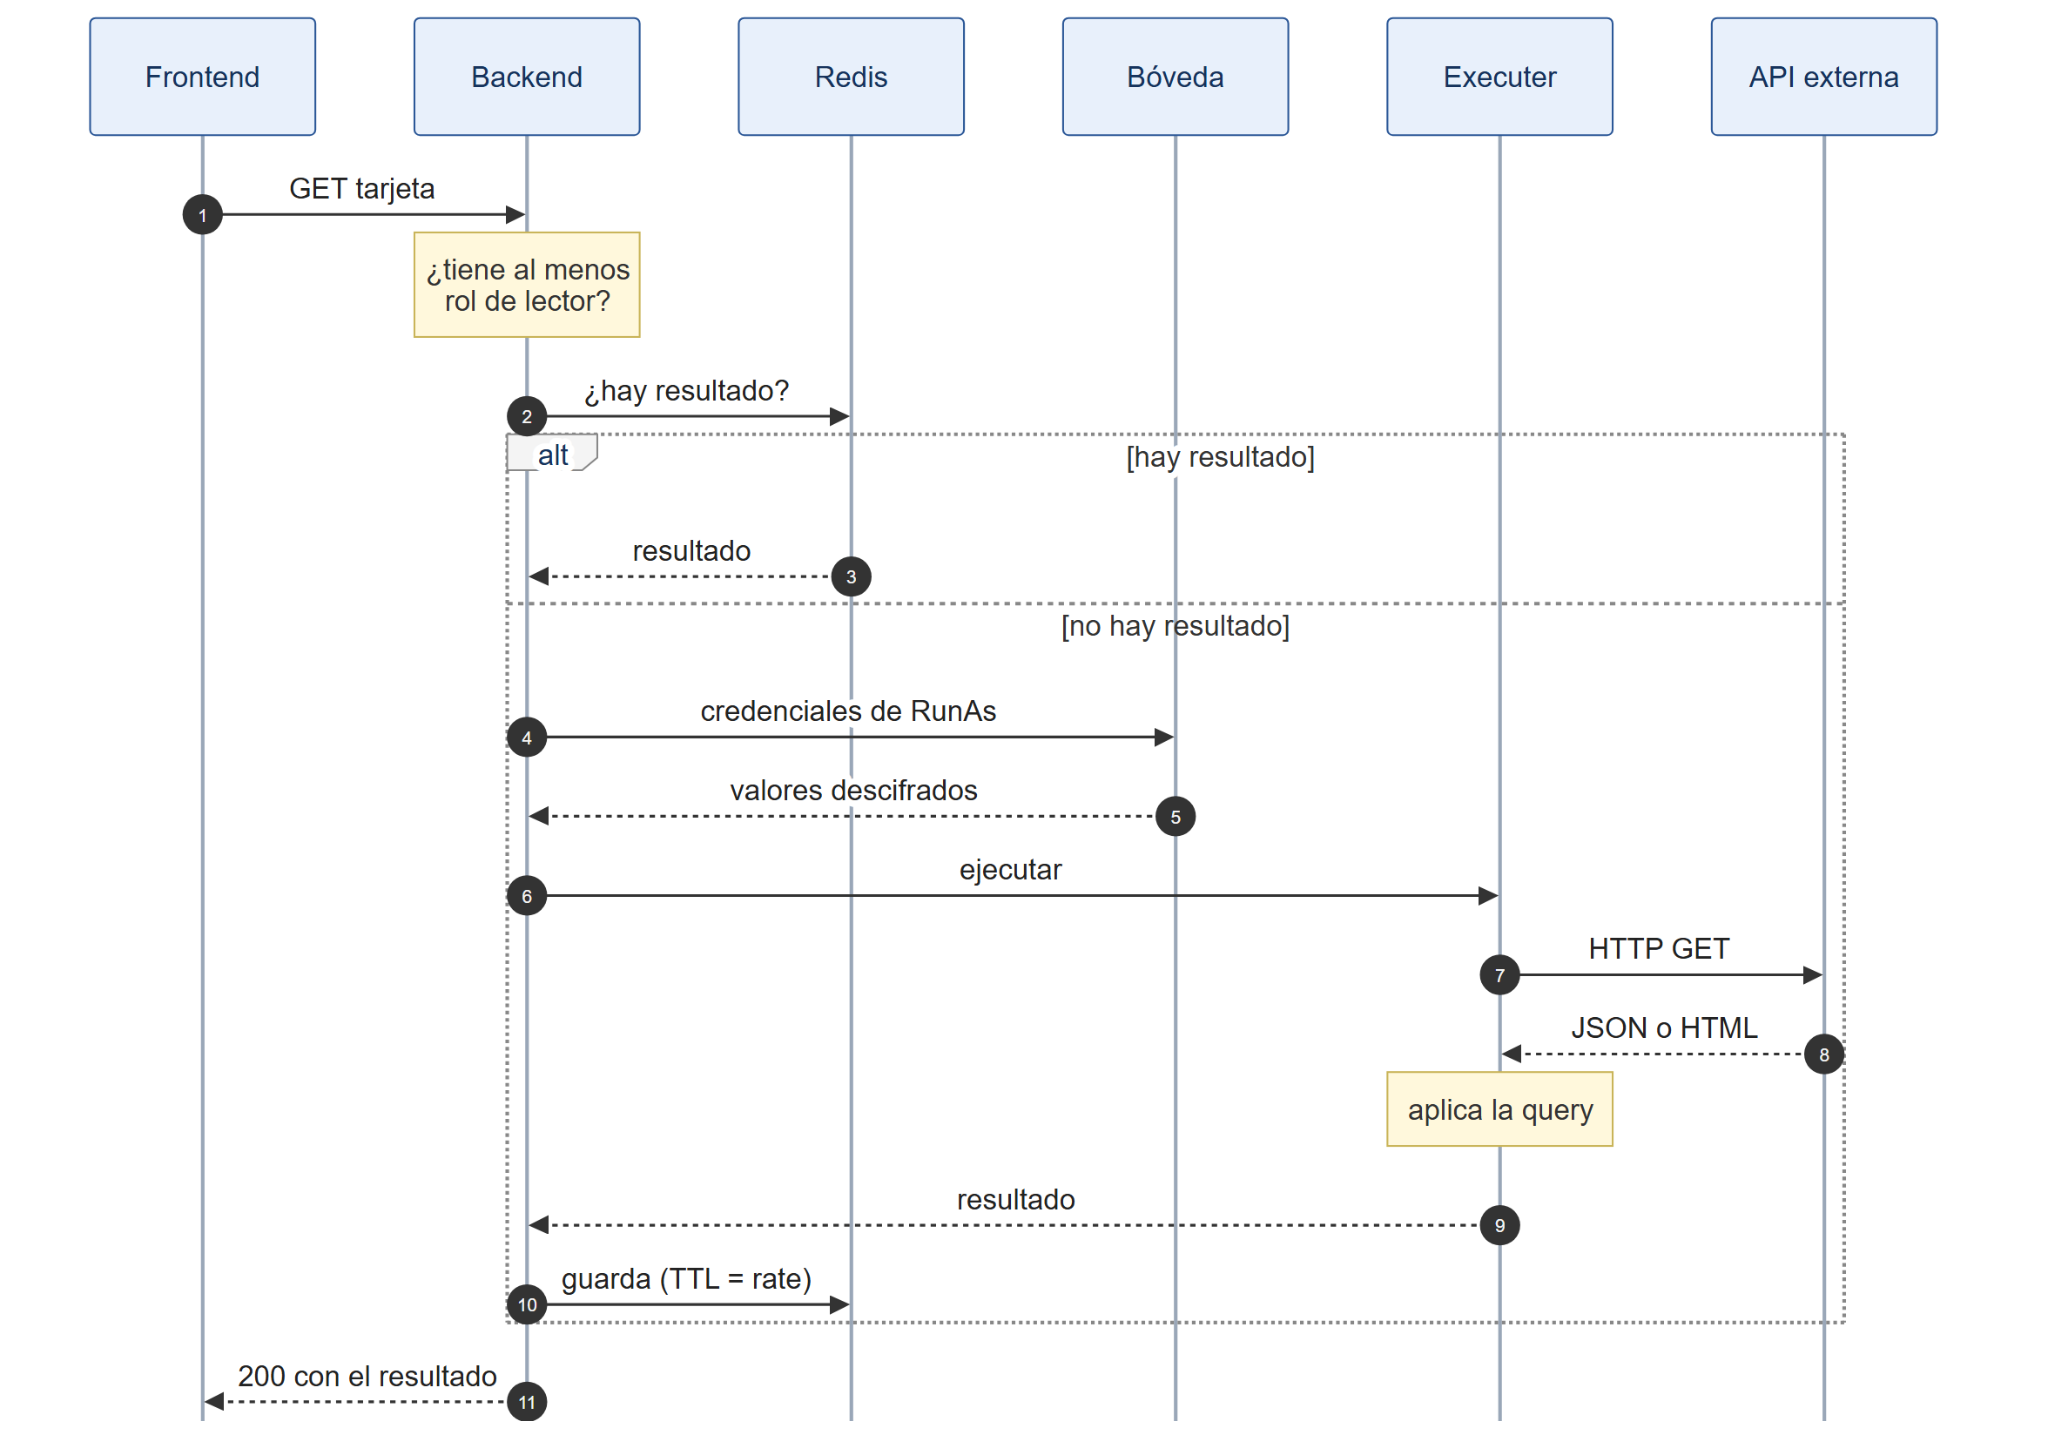
\includegraphics[width=0.95\textwidth]{figuras/fig10.png}
  \caption{Diagrama de secuencia de la ejecución de una tarjeta}
  \label{fig:seq_ejecucion}
\end{figure}

\subsection{Edición Colaborativa en Tiempo Real}
El mecanismo de edición colaborativa en tiempo real se diagramó en la Figura~\ref{fig:seq_realtime} y se desarrolla a través de dos canales de comunicación independientes.

Cuando un usuario abre un tablero, el frontend establece una conexión con el servicio de tiempo real y le proporciona su token de acceso. El servicio de tiempo real utiliza ese token para consultar al backend y verificar los permisos del usuario sobre el tablero. Una vez autorizada la conexión, registra la presencia del usuario en Redis y le envía la lista de participantes conectados. A partir de esta información, los navegadores establecen conexiones WebRTC entre sí, mediante las cuales comparten cursores y movimientos de arrastre directamente, sin que estos datos deban pasar por el servidor.

Por otro lado, cuando un usuario con permisos de edición modifica el tablero, el backend persiste los cambios en MongoDB. El servicio de tiempo real escucha directamente el Change Stream de la colección de tableros, configurado para recibir únicamente operaciones de actualización. Ante cada modificación, MongoDB proporciona el documento completo del tablero en su estado actualizado. El servicio de tiempo real recibe este evento y distribuye el tablero actualizado a todos los participantes.

Finalmente, un minuto antes del vencimiento del token de acceso, el servicio de tiempo real solicita su renovación y vuelve a verificar los permisos del usuario. Si el usuario fue removido del tablero, el servicio interrumpe su conexión y deja de enviarle actualizaciones. De esta manera, un participante removido pierde el acceso a las actualizaciones en tiempo real a más tardar durante el siguiente proceso de renovación del token.

\begin{figure}[H]
  \centering
  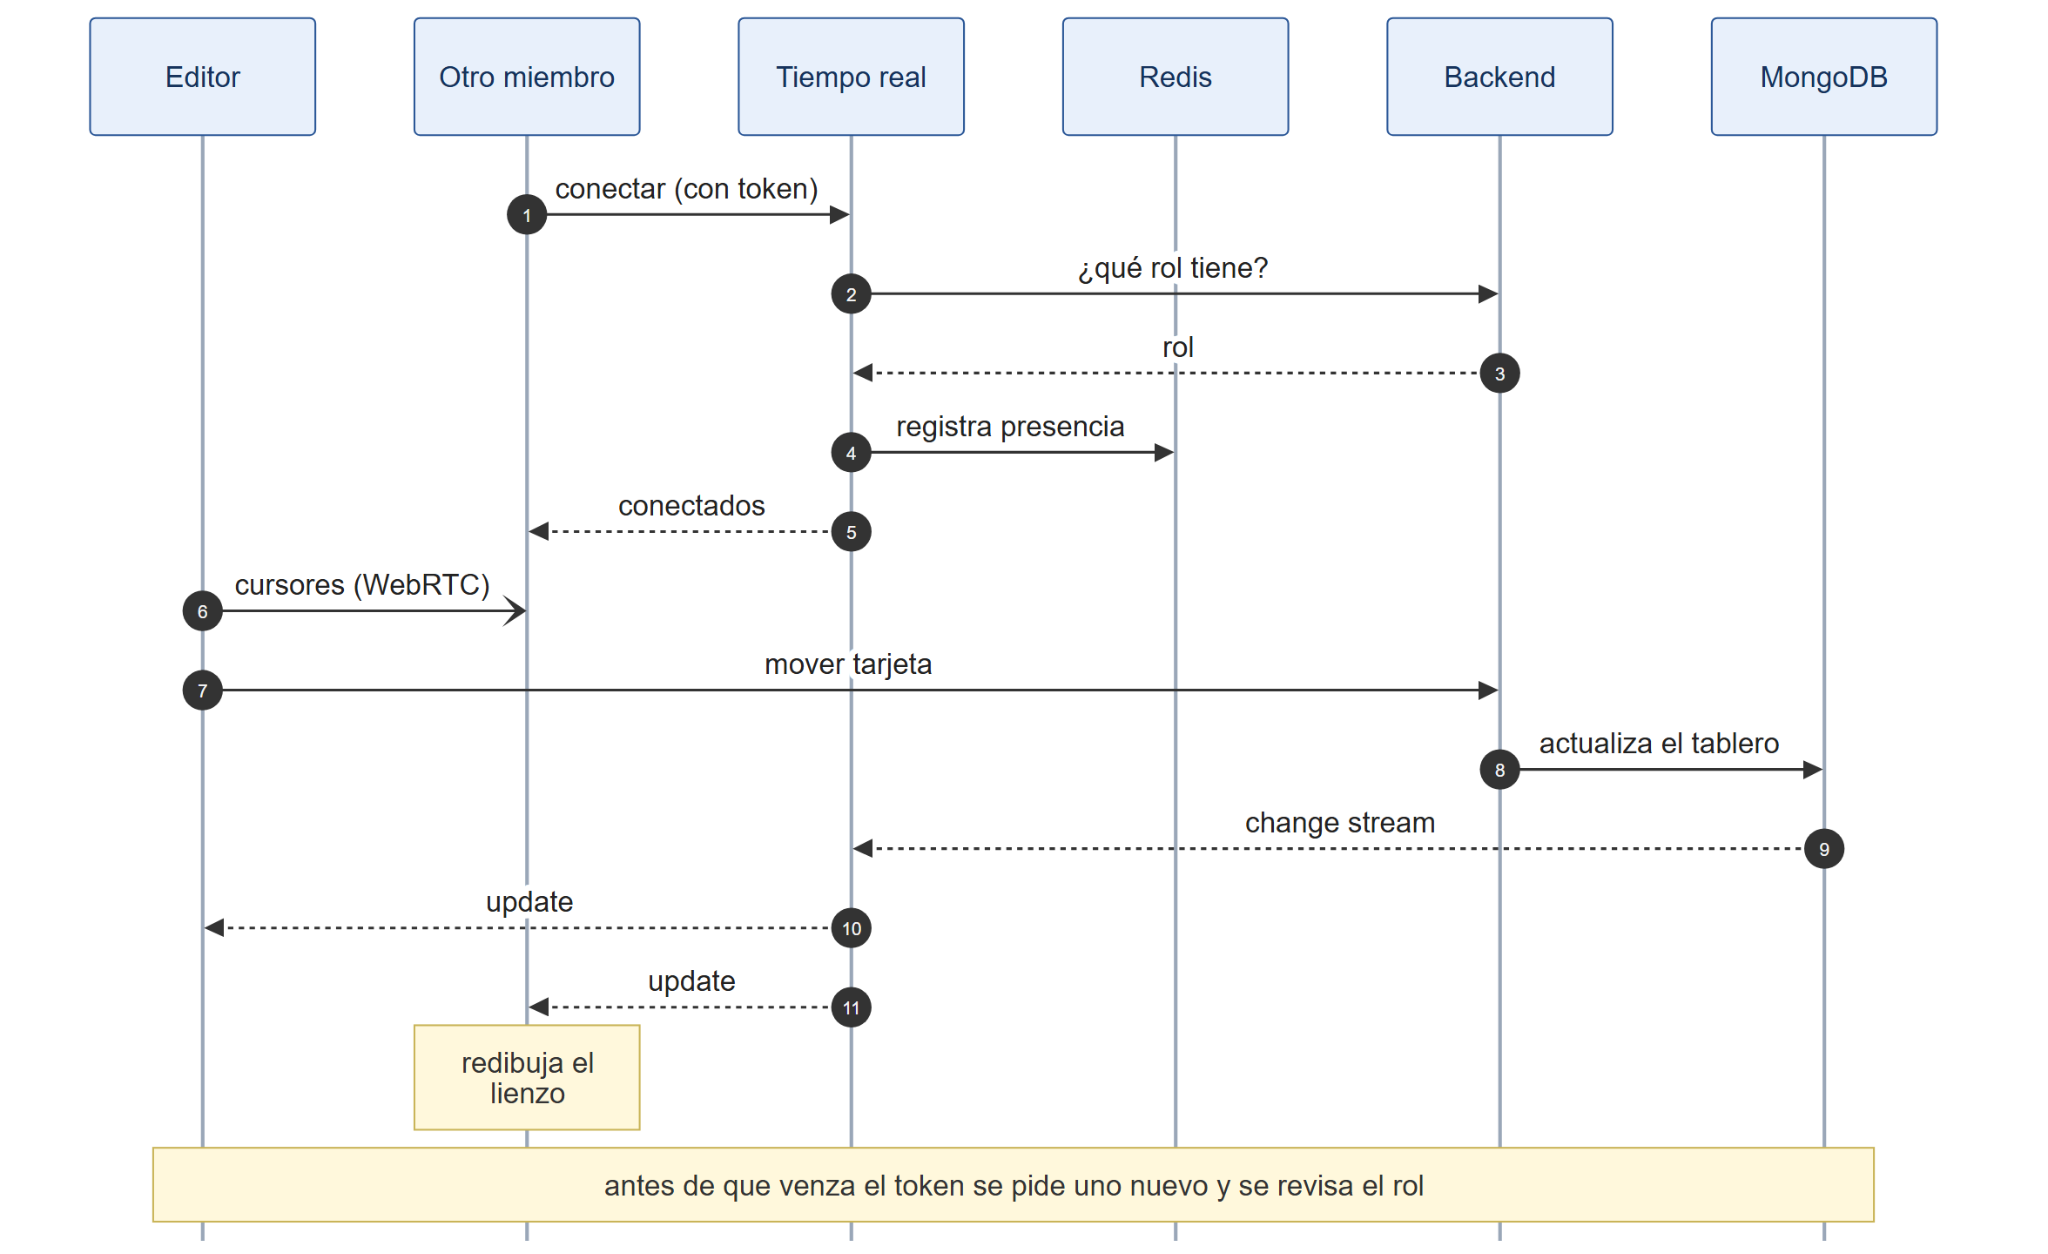
\includegraphics[width=0.95\textwidth]{figuras/fig11.png}
  \caption{Diagrama de secuencia de la edición colaborativa en tiempo real}
  \label{fig:seq_realtime}
\end{figure}

\subsection{Uso de servidor MCP}
La Figura~\ref{fig:seq_mcp} esquematiza la interacción de un agente de inteligencia artificial con el sistema a través del servidor MCP. En primer lugar, el desarrollador genera desde su perfil un token personal (con el prefijo \texttt{tiu\_pat\_}), cuyo vencimiento puede configurarse en 7, 15 o 30 días, cada usuario puede tener hasta diez tokens activos, los cuales nunca se renueva. Por motivos de seguridad, el backend almacena únicamente el hash SHA-256 del token, sin conservar su valor original. El acceso por token es una funcionalidad de los planes pagos.

Para interactuar con el sistema, el agente de IA proporciona el token personal al servidor MCP, que expone las herramientas disponibles y traduce cada invocación en una o más llamadas a la API REST del backend, reenviando el token sin almacenarlo. El servidor presenta cada tablero como un grafo de conocimiento personal, cada tarjeta como una memoria y cada hilo como una asociación entre memorias. Las herramientas permiten listar, crear y eliminar tableros (\texttt{list\_pkgs}, \texttt{create\_pkg} y \texttt{delete\_pkg}), listar las memorias de un tablero (\texttt{memories}), guardar una memoria de texto (\texttt{consolidate}), modificarla (\texttt{reconsolidate}) y eliminarla (\texttt{forget}), y vincular memorias o desvincularlas (\texttt{associate} y \texttt{dissociate}), nombrando la relación y su dirección. La herramienta \texttt{perceive} guarda una memoria viva: una tarjeta personalizada que consulta una API o una página web mediante \texttt{GET} o \texttt{POST} y se actualiza periódicamente. Las credenciales nunca pasan por el agente, que las referencia como \texttt{\$NOMBRE} para que el backend las resuelva desde la bóveda del tablero. Finalmente, \texttt{retrieve} recupera una memoria con sus datos actualizados, cómo se obtienen si es una memoria viva y las memorias relacionadas, indicando la dirección y la etiqueta de cada relación.

El backend autentica las solicitudes mediante el token personal y las restringe a una lista explícita de rutas: la lectura de tableros, tarjetas, organizaciones, el perfil y el catálogo de integraciones, y la creación, edición y eliminación de tableros, tarjetas e hilos. Cualquier otra ruta, como la gestión de secretos, el uso compartido, los tokens o la facturación, responde 403. Además, aplica los roles que el usuario posee sobre cada tablero, de modo que el agente no puede realizar operaciones que excedan los permisos de su propietario.

\begin{figure}[H]
  \centering
  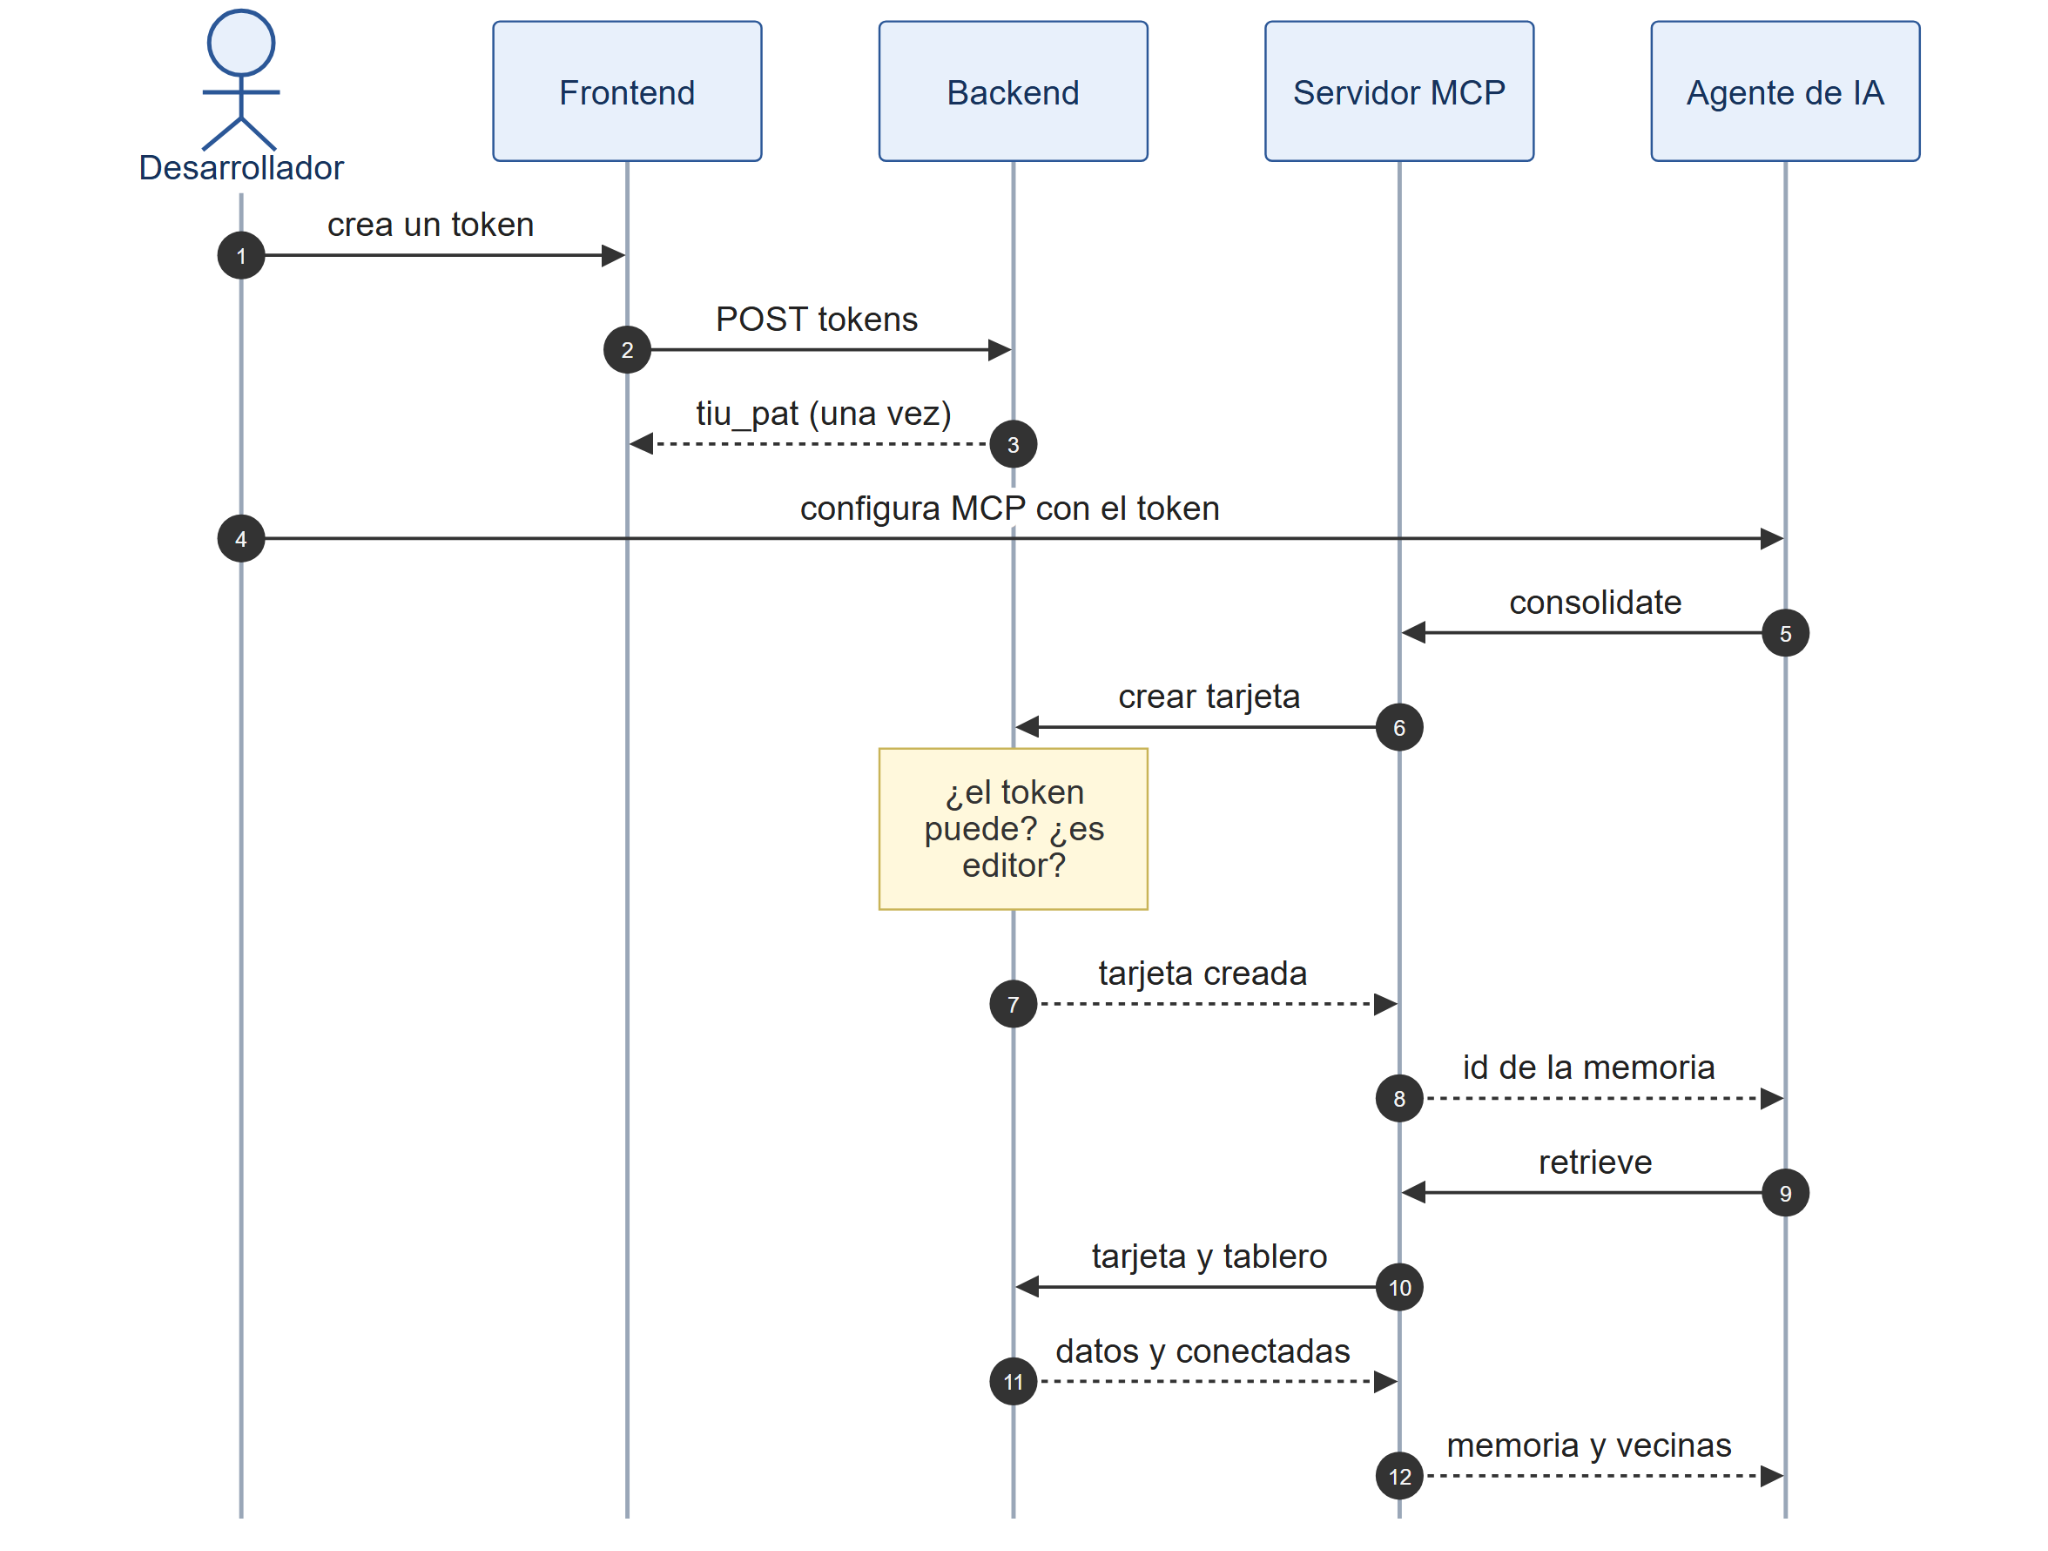
\includegraphics[width=0.95\textwidth]{figuras/fig12.png}
  \caption{Diagrama de secuencia del uso por parte de un agente de IA}
  \label{fig:seq_mcp}
\end{figure}

\subsection{Conexión OAuth2}
La Figura~\ref{fig:seq_oauth2} describe el proceso de vinculación de una cuenta externa mediante OAuth2. En primer lugar, el backend genera la URL de consentimiento y almacena en Redis el estado del intercambio, asociado al usuario que inició el proceso. Luego, el proveedor OAuth2 redirige al frontend con el código de autorización, que este reenvía al backend para completar el intercambio.

Al recibir el código, el backend verifica que el usuario que intenta completar el proceso sea el mismo que lo inició. Si la validación es satisfactoria, el backend intercambia el código por los correspondientes tokens de acceso y los almacena cifrados mediante la clave de datos del ámbito seleccionado. En ningún momento los tokens son enviados al frontend.

\begin{figure}[H]
  \centering
  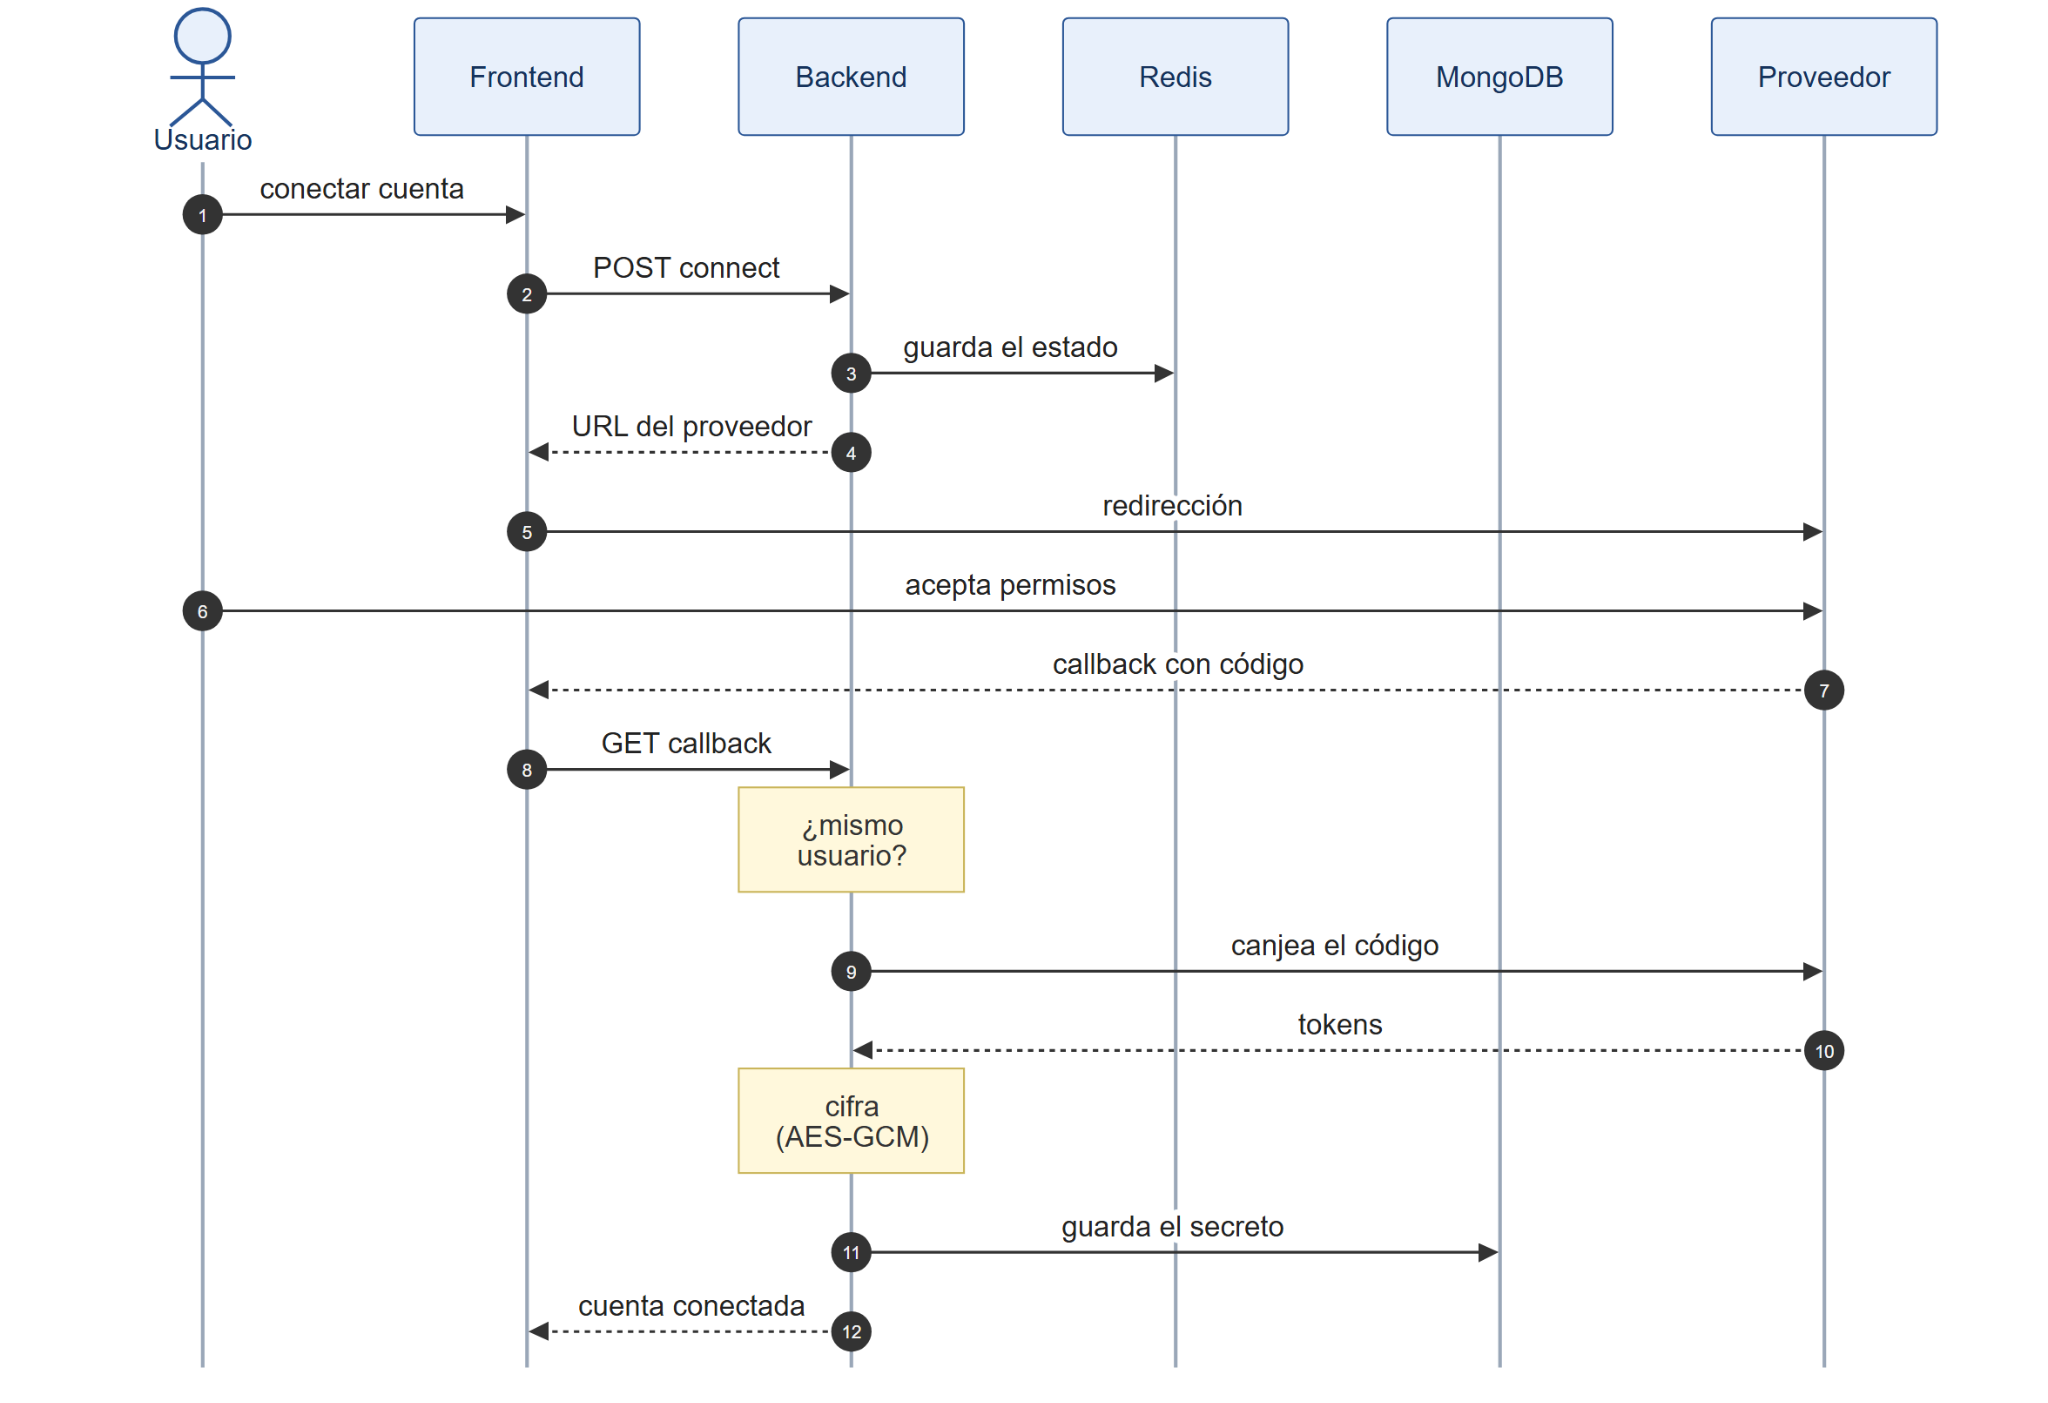
\includegraphics[width=0.95\textwidth]{figuras/fig13.png}
  \caption{Diagrama de secuencia de la conexión de una cuenta mediante OAuth2}
  \label{fig:seq_oauth2}
\end{figure}

\section{Diseño de la base de datos}
A continuación se detallan las colecciones principales de MongoDB. Para cada campo se especifica su tipo físico BSON, si se encuentra indexado y una breve descripción de su propósito, indicando cuando corresponde si se trata de una referencia a otra colección o de un objeto embebido.

\subsection{Colección: boards}
La siguiente colección almacena la metadata del tablero, sus miembros con el rol de cada uno, las relaciones visuales entre elementos (strands) y una lista optimizada de los post-its activos.

\begin{tablacoleccion}{Colección \texttt{boards} MongoDB}{tab:col_boards}
  \_id & binData (UUID) & Sí (Primary) & Identificador único del tablero. \\
  name & string & No & Nombre visible del tablero. \\
  owner & string & Sí & ID del usuario creador (referencia a \texttt{users}). \\
  members & array (objects) & Sí (\texttt{members.user}) & Usuarios con acceso al tablero, cada uno con su rol. \\
  members[].user & string & Sí & ID del miembro (referencia a \texttt{users}). \\
  members[].role & string & No & Rol del miembro: \texttt{editor} o \texttt{viewer}. \\
  org & binData (UUID) & Sí & Organización a la que pertenece el tablero (referencia a \texttt{orgs}). Opcional. \\
  postits & array (objects) & No & Estructura embebida con datos de renderizado de los post-its. Los campos de estilo de cada tarjeta son opcionales y un valor por defecto no se almacena. \\
  postits[].id & binData (UUID) & No & ID de la configuración completa en la colección \texttt{postit}. \\
  postits[].type & string & No & Clave de la integración o plantilla de la que proviene la tarjeta (vacía en una tarjeta personalizada); el frontend la usa para elegir cómo dibujarla. \\
  postits[].title & object & No & Título de la tarjeta (\texttt{text}) y si interpola variables del resultado (\texttt{vars}). \\
  postits[].position & object & No & Coordenadas x/y de la tarjeta dentro del lienzo. \\
  postits[].color & string & No & Color de fondo de la tarjeta: la paleta de los hilos o \texttt{white}. Opcional. \\
  postits[].border & string & No & Borde de la tarjeta: \texttt{none}, \texttt{solid}, \texttt{dashed} o \texttt{dotted}. Opcional. \\
  postits[].border\_width & string & No & Grosor del borde: \texttt{thin}, \texttt{normal} o \texttt{thick}. Opcional. \\
  postits[].border\_color & string & No & Color del borde, con las mismas opciones que \texttt{color}; si falta, sigue el color de la tarjeta. Opcional. \\
  postits[].text\_align & string & No & Alineación horizontal del texto: \texttt{left}, \texttt{center} o \texttt{right}. Opcional. \\
  postits[].vertical\_align & string & No & Ubicación vertical del texto: \texttt{top}, \texttt{middle} o \texttt{bottom}; se nota en una tarjeta con alto propio. Opcional. \\
  postits[].width & double & No & Ancho de la tarjeta en píxeles del lienzo, entre 120 y 1600. Opcional. \\
  postits[].height & double & No & Alto de la tarjeta en píxeles del lienzo, entre 60 y 1200. Opcional. \\
  strands & array (objects) & No & Lista de conexiones o hilos entre post-its. Los campos de estilo de cada hilo son opcionales y un valor por defecto no se almacena. \\
  strands[].id & binData (UUID) & No & Identificador único del hilo. \\
  strands[].source & binData (UUID) & No & Post-it de origen del hilo. \\
  strands[].target & binData (UUID) & No & Post-it de destino del hilo. \\
  strands[].label & string & No & Etiqueta que describe la relación, de hasta 80 caracteres. Opcional. \\
  strands[].arrow & string & No & Flechas del hilo: \texttt{none}, \texttt{start}, \texttt{end} o \texttt{both}. Opcional. \\
  strands[].width & string & No & Grosor del hilo: \texttt{thin}, \texttt{normal} o \texttt{thick}. Opcional. \\
  strands[].color & string & No & Color de una paleta fija: \texttt{gray}, \texttt{red}, \texttt{orange}, \texttt{yellow}, \texttt{green}, \texttt{blue}, \texttt{purple} o \texttt{pink}. Opcional. \\
  envs & array (objects) & No & Variables de entorno compartidas en el tablero. \\
\end{tablacoleccion}

\subsection{Colección: postit}
La siguiente colección contiene la configuración dinámica, los parámetros de integración y los datos de peticiones HTTP de forma autocontenida para cada elemento de un PostIt.

\begin{tablacoleccion}{Colección \texttt{postit} MongoDB}{tab:col_postits}
  \_id & binData (UUID) & Sí (Primary) & Identificador único del post-it. \\
  board & binData (UUID) & Sí & ID del tablero al que pertenece (referencia inversa). \\
  wellknown & string & No & Clave de la integración predefinida de la que proviene, si corresponde. \\
  query & object (map) & No & Mapa clave-expresión con las proyecciones a aplicar (\texttt{jq} para JSON, selectores CSS para HTML). \\
  rate & int & No & Tiempo de vida del resultado en caché, expresado en segundos. \\
  envs & array (objects) & No & Variables de entorno propias del post-it. \\
  runas & string & No & ID del usuario cuya identidad se utiliza para resolver las credenciales (referencia a \texttt{users}). \\
  bindings & object (map) & No & Mapa de placeholder a referencia de secreto (\texttt{\{scope, name\}}) en la colección \texttt{secrets}. \\
  params & object (map) & No & Esquema dinámico de pares clave-valor según el tipo de post-it. \\
  resource & string & No & URL del endpoint o recurso externo asociado. \\
  request & object & No & Documento embebido con la estructura de la petición HTTP (\texttt{method}, \texttt{headers}, \texttt{queries}, \texttt{body}). \\
  response & string & No & Tipo de respuesta de la API (JSON o HTML), utilizado para elegir el intérprete de la query. \\
\end{tablacoleccion}

\subsection{Colección: users}
La siguiente colección almacena las cuentas de usuario junto con las identidades con las que cada una puede iniciar sesión.

\begin{tablacoleccion}{Colección \texttt{users} MongoDB}{tab:col_users}
  \_id & binData (UUID) & Sí (Primary) & Identificador único del usuario; es el \texttt{sub} del token de acceso. \\
  email & string & Sí (único) & Correo electrónico normalizado. \\
  emailverified & bool & No & Indica si el correo fue verificado mediante el enlace enviado. \\
  name & string & No & Nombre visible. \\
  picture & string & No & URL de la foto de perfil. \\
  locale & string & No & Idioma preferido (\texttt{en} o \texttt{es}), utilizado para los correos. \\
  admin & bool & No & Indica si es administrador de la plataforma (derivado de \texttt{PLATFORM\_ADMINS}). \\
  identities & array (objects) & No & Identidades vinculadas: \texttt{provider} (\texttt{password} o \texttt{google}), \texttt{subject} y hash \texttt{argon2id}. \\
  identitykeys & array (objects) & Sí (único, parcial) & Claves \texttt{provider:subject} que impiden vincular una misma cuenta externa a dos usuarios. \\
  plan & string & No & Plan contratado: \texttt{free}, \texttt{pro} o \texttt{max}. Vacío equivale a \texttt{free}. Opcional. \\
  plan\_expires & date & No & Vencimiento del plan. Si está vencido, el plan vuelve a \texttt{free}. Con una suscripción activa es la fecha del próximo pago más cinco días de gracia. Opcional. \\
  createdat & date & No & Fecha de alta. \\
  updatedat & date & No & Última fecha de modificación. \\
\end{tablacoleccion}

\subsection{Colección: orgs}
La siguiente colección modela las organizaciones, que funcionan como un tenant mínimo: un tablero o grupo creado dentro de una organización alcanza a todos sus miembros sin necesidad de compartirlo.

\begin{tablacoleccion}{Colección \texttt{orgs} MongoDB}{tab:col_orgs}
  \_id & binData (UUID) & Sí (Primary) & Identificador único de la organización. \\
  name & string & No & Nombre visible. \\
  members & array (objects) & Sí (\texttt{members.user}) & Miembros con su rol (\texttt{admin} o \texttt{member}). \\
  owner & string & Sí & Usuario que paga la organización (referencia a \texttt{users}). Los límites de los tableros de la organización provienen de su plan. Opcional. \\
  createdat & date & No & Fecha de alta. \\
\end{tablacoleccion}

\subsection{Colección: groups}
La siguiente colección almacena los grupos de usuarios, cuya función principal es ser propietarios de secretos compartidos entre varias personas.

\begin{tablacoleccion}{Colección \texttt{groups} MongoDB}{tab:col_groups}
  \_id & binData (UUID) & Sí (Primary) & Identificador único del grupo. \\
  name & string & No & Nombre visible. \\
  owner & string & Sí & ID del creador (referencia a \texttt{users}). \\
  members & array (strings) & Sí & IDs de los miembros (referencia a \texttt{users}). \\
  org & binData (UUID) & Sí & Organización a la que pertenece (referencia a \texttt{orgs}). Opcional. \\
  createdat & date & No & Fecha de alta. \\
\end{tablacoleccion}

\subsection{Colección: secrets}
La siguiente colección conforma la bóveda de credenciales. Cada secreto se identifica por el par \texttt{(scope, name)} y su valor se almacena cifrado; ningún endpoint devuelve el valor en claro.

\begin{tablacoleccion}{Colección \texttt{secrets} MongoDB}{tab:col_secrets}
  \_id & binData (UUID) & Sí (Primary) & Identificador único del secreto. \\
  scope & object & Sí (único con \texttt{name}) & Ámbito del secreto: \texttt{kind} (\texttt{board}, \texttt{member}, \texttt{user}, \texttt{group} o \texttt{system}) y \texttt{owner}. \\
  name & string & Sí (único con \texttt{scope}) & Nombre en mayúsculas con el que se referencia desde una tarjeta (\texttt{\$NOMBRE}). \\
  kind & string & No & Tipo de credencial: \texttt{api\_key}, \texttt{bearer}, \texttt{basic}, \texttt{oauth2} u \texttt{oauth2\_client}. \\
  ciphertext & binData & No & Valor cifrado con AES-GCM. \\
  nonce & binData & No & Nonce utilizado en el cifrado. \\
  keyid & binData (UUID) & No & Clave de datos con la que se cifró (referencia a \texttt{data\_keys}). \\
  flow & string & No & Flujo OAuth2 (\texttt{client\_credentials} o \texttt{authorization\_code}), si corresponde. \\
  authorized & bool & No & Indica si el consentimiento OAuth2 fue completado. \\
  provider & string & No & Proveedor de plataforma (\texttt{google}, \texttt{discord}, etc.) para conexiones administradas. \\
  grants & array (objects) & Sí (\texttt{grants.to.kind}, \texttt{grants.to.id}) & Permisos de uso otorgados a un usuario, grupo o tablero, opcionalmente limitados a un tablero. \\
  billed\_to & string & Sí & Usuario a cuyo plan se descuenta el secreto (referencia a \texttt{users}). Opcional. \\
  createdat & date & No & Fecha de alta. \\
  updatedat & date & No & Fecha de última modificación. \\
\end{tablacoleccion}

\subsection{Colección: data\_keys}
La siguiente colección almacena las claves de datos de cada ámbito, envueltas a su vez por la clave maestra versionada.

\begin{tablacoleccion}{Colección \texttt{data\_keys} MongoDB}{tab:col_data_keys}
  \_id & binData (UUID) & Sí (Primary) & Identificador único de la clave. \\
  scope & object & Sí (único entre las activas) & Ámbito al que pertenece la clave (\texttt{kind} y \texttt{owner}). \\
  wrappedkey & binData & No & Clave de datos cifrada con la clave maestra (KEK). \\
  nonce & binData & No & Nonce utilizado al envolver la clave. \\
  kekversion & int & No & Versión de la clave maestra que la envuelve. \\
  active & bool & No & Indica si es la clave vigente del ámbito. \\
  createdat & date & No & Fecha de alta. \\
  retiredat & date & No & Fecha de retiro tras una rotación. \\
\end{tablacoleccion}

\subsection{Colección: access\_tokens}
La siguiente colección almacena los tokens personales de acceso que los desarrolladores generan para herramientas externas, como el servidor MCP. Del token solo se guarda su hash, y un índice TTL hace que MongoDB elimine cada documento al llegar su fecha de vencimiento.

\begin{tablacoleccion}{Colección \texttt{access\_tokens} MongoDB}{tab:col_access_tokens}
  \_id & binData (UUID) & Sí (Primary) & Identificador único del token. \\
  user & string & Sí & ID del usuario al que representa el token (referencia a \texttt{users}). \\
  name & string & No & Nombre que el usuario le asigna al token. \\
  prefix & string & No & Comienzo visible del token, para reconocerlo en el perfil. \\
  hash & string & Sí (único) & Hash SHA-256 del token; el valor completo no se almacena. \\
  created\_at & date & No & Fecha de alta. \\
  expires\_at & date & Sí (TTL) & Fecha de vencimiento; al llegar a ella MongoDB elimina el documento. \\
  last\_used\_at & date & No & Fecha del último uso, si lo hubo. \\
\end{tablacoleccion}

\subsection{Colección: well\_knowns}
La siguiente colección almacena el catálogo de integraciones predefinidas. Cada documento describe cómo obtener un dato de una fuente externa y qué debe completar el usuario al crear una tarjeta a partir de él, con sus textos en español e inglés.

\begin{tablacoleccion}{Colección \texttt{well\_knowns} MongoDB}{tab:col_well_knowns}
  \_id & string & Sí (Primary) & Clave de la integración (por ejemplo, \texttt{dolar\_oficial}). \\
  name\_es / name\_en & string & No & Nombre de la integración en cada idioma. \\
  description\_es / description\_en & string & No & Descripción opcional en cada idioma. \\
  title\_es / title\_en & string & No & Título por defecto de las tarjetas creadas a partir de ella. \\
  order & int & No & Posición de la integración en el catálogo. \\
  resource & string & No & URL del recurso externo. \\
  request & object & No & Documento embebido con método, headers, queries y cuerpo de la petición. \\
  response & string & No & Tipo de respuesta (\texttt{json} o \texttt{html}), que define el intérprete de la query. \\
  query & object (map) & No & Proyecciones a aplicar sobre la respuesta. \\
  rate & int & No & Tiempo de vida del resultado en caché, expresado en segundos. \\
  parameters & array (objects) & No & Parámetros que completa el usuario: clave, etiquetas, tipo (\texttt{string}, \texttt{number} o \texttt{secret}) y valor por defecto. \\
  outputs & array (objects) & No & Salidas de la tarjeta, con su etiqueta y un ejemplo en cada idioma. \\
  system\_secrets & object (map) & No & Secretos de sistema que se inyectan al ejecutar la tarjeta. \\
  builtin & bool & No & Indica si es una integración incorporada al sistema. \\
  deleted & bool & No & Marca de eliminación lógica. \\
  updated\_at & date & No & Fecha de la última modificación. \\
  updated\_by & string & No & Administrador que realizó la última modificación (referencia a \texttt{users}). \\
\end{tablacoleccion}

\subsection{Colección: postit\_templates}
La siguiente colección almacena las plantillas de tarjeta que definen los usuarios. Cada plantilla pertenece a un usuario, a un tablero o a una organización, y tiene la misma estructura de petición que una integración del catálogo.

\begin{tablacoleccion}{Colección \texttt{postit\_templates} MongoDB}{tab:col_postit_templates}
  \_id & string & Sí (Primary) & Clave de la plantilla, con el prefijo \texttt{custom\_}. \\
  scope & object & Sí (con \texttt{name}) & Ámbito al que pertenece: \texttt{kind} (\texttt{user}, \texttt{board} u \texttt{org}) y \texttt{owner}. \\
  name & string & Sí (con \texttt{scope}) & Nombre de la plantilla. \\
  description & string & No & Descripción opcional. \\
  title & object & No & Título por defecto de las tarjetas creadas a partir de ella. \\
  resource & string & No & URL del recurso externo. \\
  request & object & No & Documento embebido con método, headers, queries y cuerpo de la petición. \\
  response & string & No & Tipo de respuesta (\texttt{json} o \texttt{html}). \\
  query & object (map) & No & Proyecciones a aplicar sobre la respuesta. \\
  rate & int & No & Tiempo de vida del resultado en caché, expresado en segundos. \\
  parameters & array (objects) & No & Parámetros que completa el usuario: clave, etiqueta, tipo y valor por defecto. \\
  outputs & array (objects) & No & Salidas de la tarjeta, con su etiqueta y un ejemplo. \\
  created\_by & string & No & Usuario que creó la plantilla (referencia a \texttt{users}). \\
  created\_at & date & No & Fecha de alta. \\
  updated\_by & string & No & Usuario que realizó la última modificación (referencia a \texttt{users}). \\
  updated\_at & date & No & Fecha de la última modificación. \\
\end{tablacoleccion}

\subsection{Colección: subscriptions}
La siguiente colección registra las suscripciones de los planes pagos. Cada documento refleja una suscripción mensual de Mercado Pago, que el backend vuelve a leer del proveedor ante cada notificación, de modo que el proveedor es siempre la fuente de verdad.

\begin{tablacoleccion}{Colección \texttt{subscriptions} MongoDB}{tab:col_subscriptions}
  \_id & string & Sí (Primary) & Identificador de la suscripción en Mercado Pago (preapproval). \\
  user & string & Sí (con \texttt{created\_at}) & Usuario suscripto (referencia a \texttt{users}). \\
  plan & string & No & Plan cobrado: \texttt{pro} o \texttt{max}. \\
  pending\_plan & string & No & Plan inferior que se aplicará con la próxima factura pagada. Opcional. \\
  status & string & No & Estado en el proveedor: \texttt{pending}, \texttt{authorized}, \texttt{paused} o \texttt{canceled}. \\
  amount\_ars & int & No & Monto mensual en pesos argentinos. \\
  next\_payment & date & No & Fecha del próximo cobro. Opcional. \\
  created\_at & date & Sí (con \texttt{user}) & Fecha de alta. \\
  updated\_at & date & No & Fecha de la última modificación. \\
\end{tablacoleccion}

\section{Modelo de dominio}

\subsection{Vista General}
A continuación se presenta una vista general del modelo de dominio, en la cual las entidades se agrupan por color en cuatro áreas: tableros y tarjetas, identidad, bóveda de secretos y planes. Las líneas punteadas indican relaciones opcionales. El usuario es la entidad hacia la que confluyen las demás: es dueño o miembro de tableros y grupos, integra organizaciones, es la identidad con la que se ejecuta cada tarjeta y a quién representa cada token personal.

\begin{figure}[H]
  \centering
  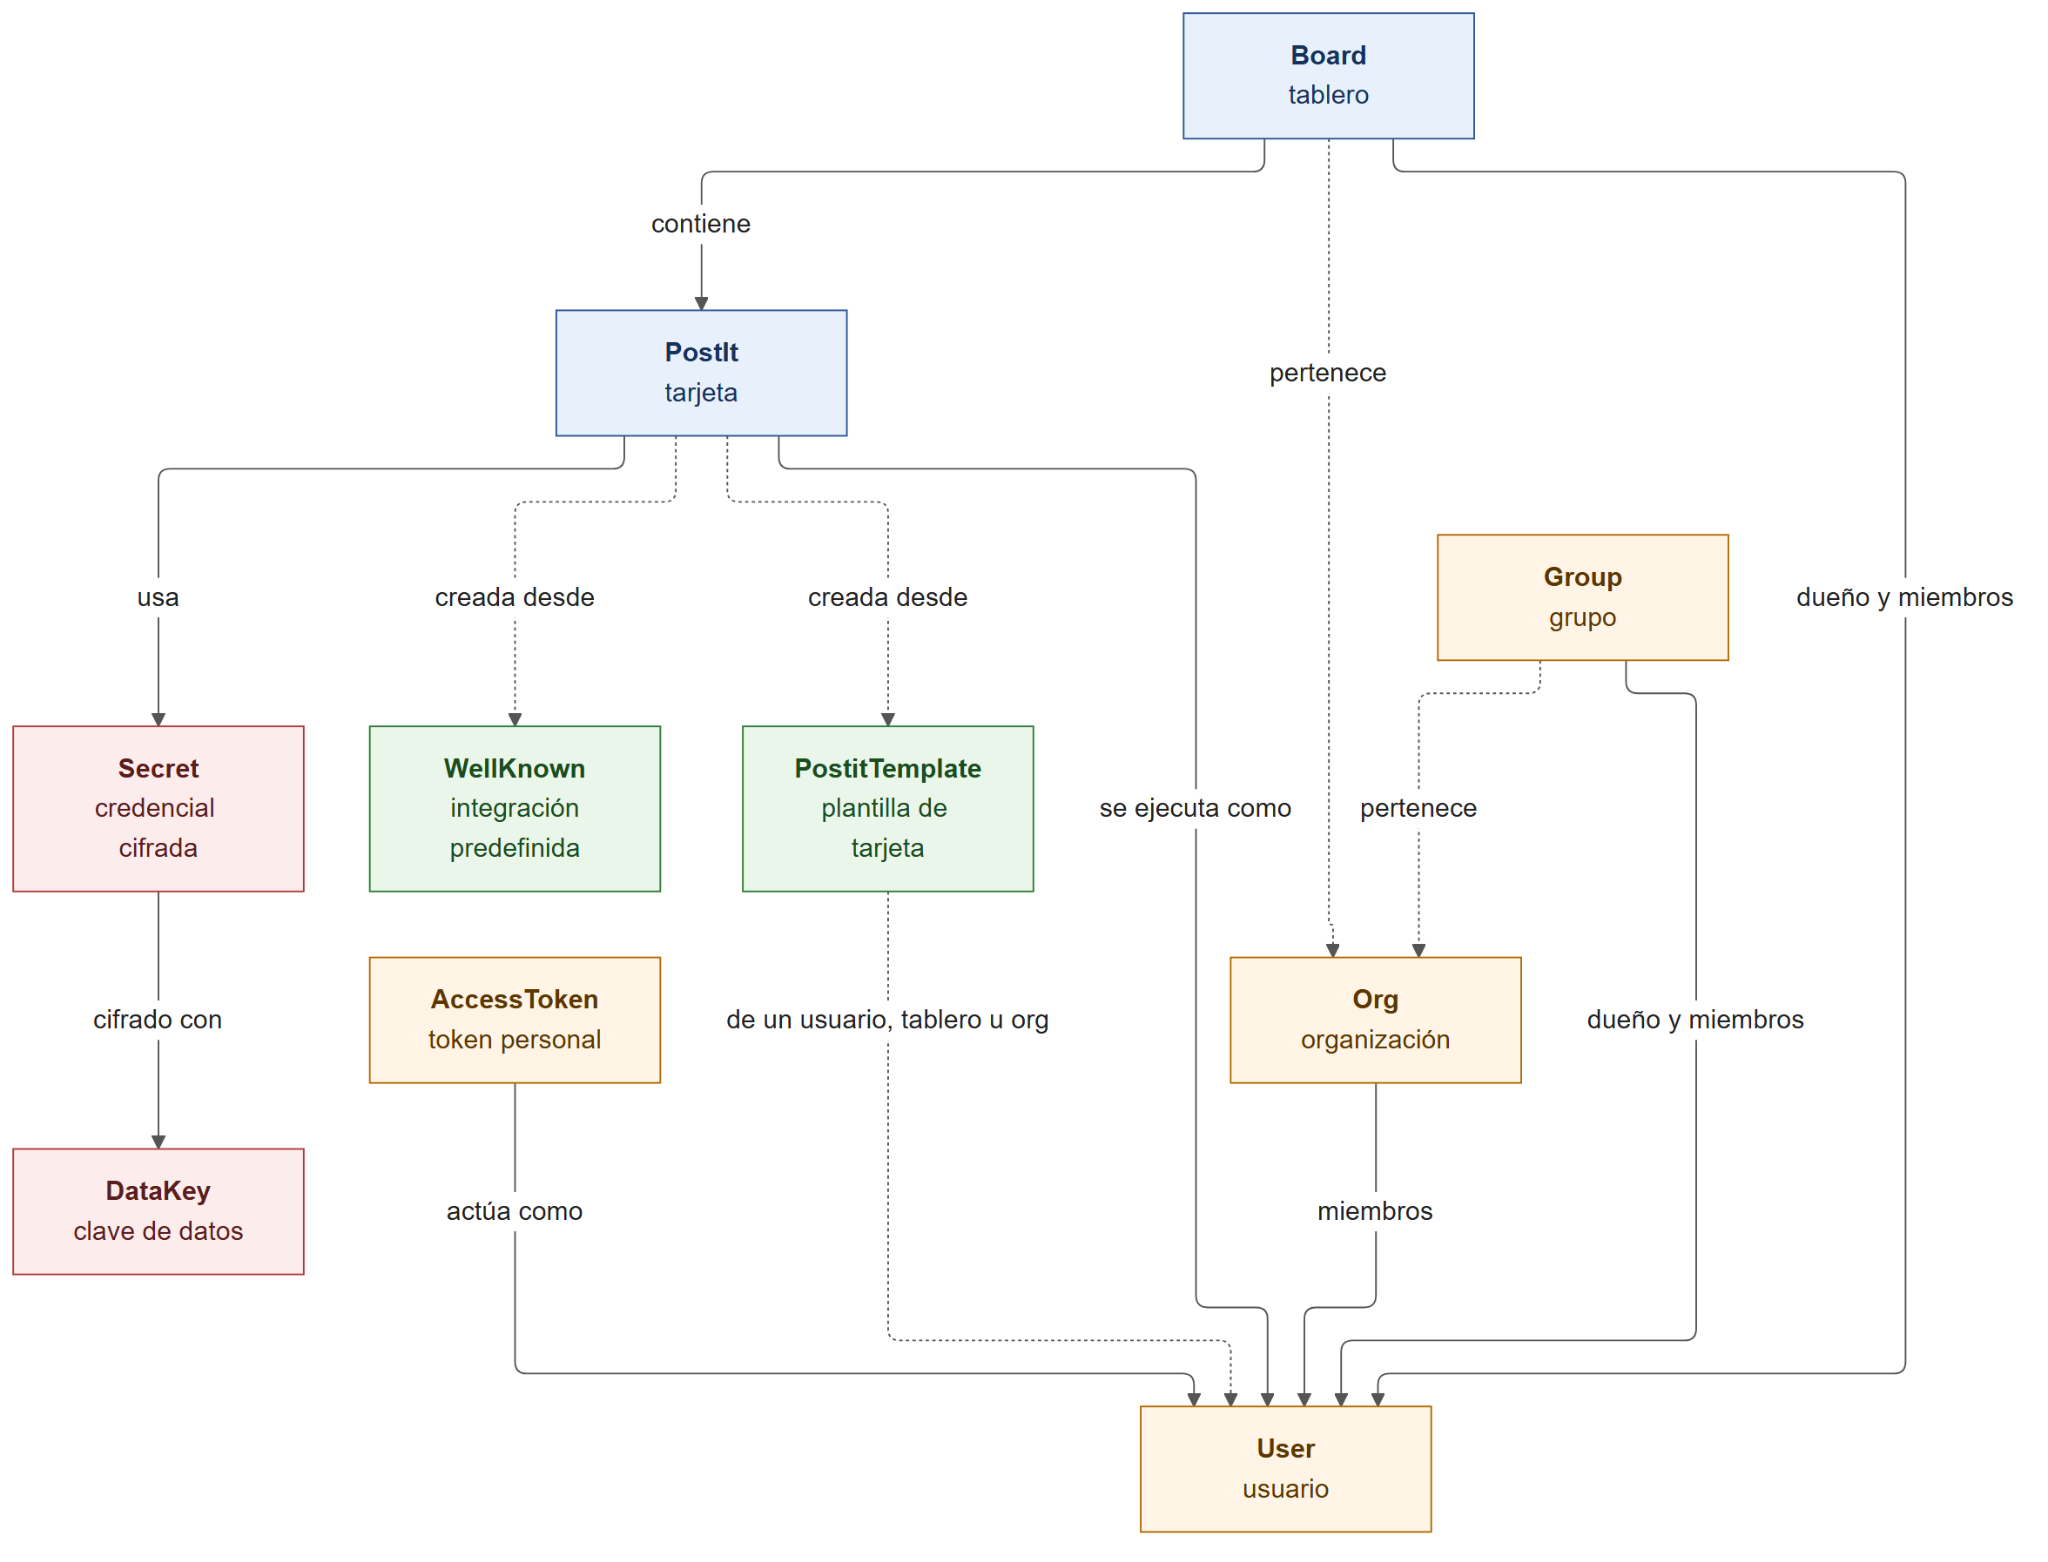
\includegraphics[width=0.95\textwidth]{figuras/fig14.png}
  \caption{Vista general del modelo de dominio}
  \label{fig:modelo_dominio_general}
\end{figure}

\subsection{Tableros y Tarjetas}
La Figura~\ref{fig:modelo_tableros_tarjetas} a continuación detalla el área de tableros, en la cual el tablero embebe a sus miembros con su rol, la posición de cada tarjeta en el lienzo (\texttt{BoardPostIt}) y los hilos que las unen (\texttt{Strand}) con su etiqueta, flechas, grosor y color opcionales, mientras que la configuración de cada tarjeta se guarda en la colección \texttt{postit} con el mismo identificador. Esta separación hace que mover una tarjeta o dibujar un hilo modifique solo el documento del tablero, que es el que observa el servicio de tiempo real.

\begin{figure}[H]
  \centering
  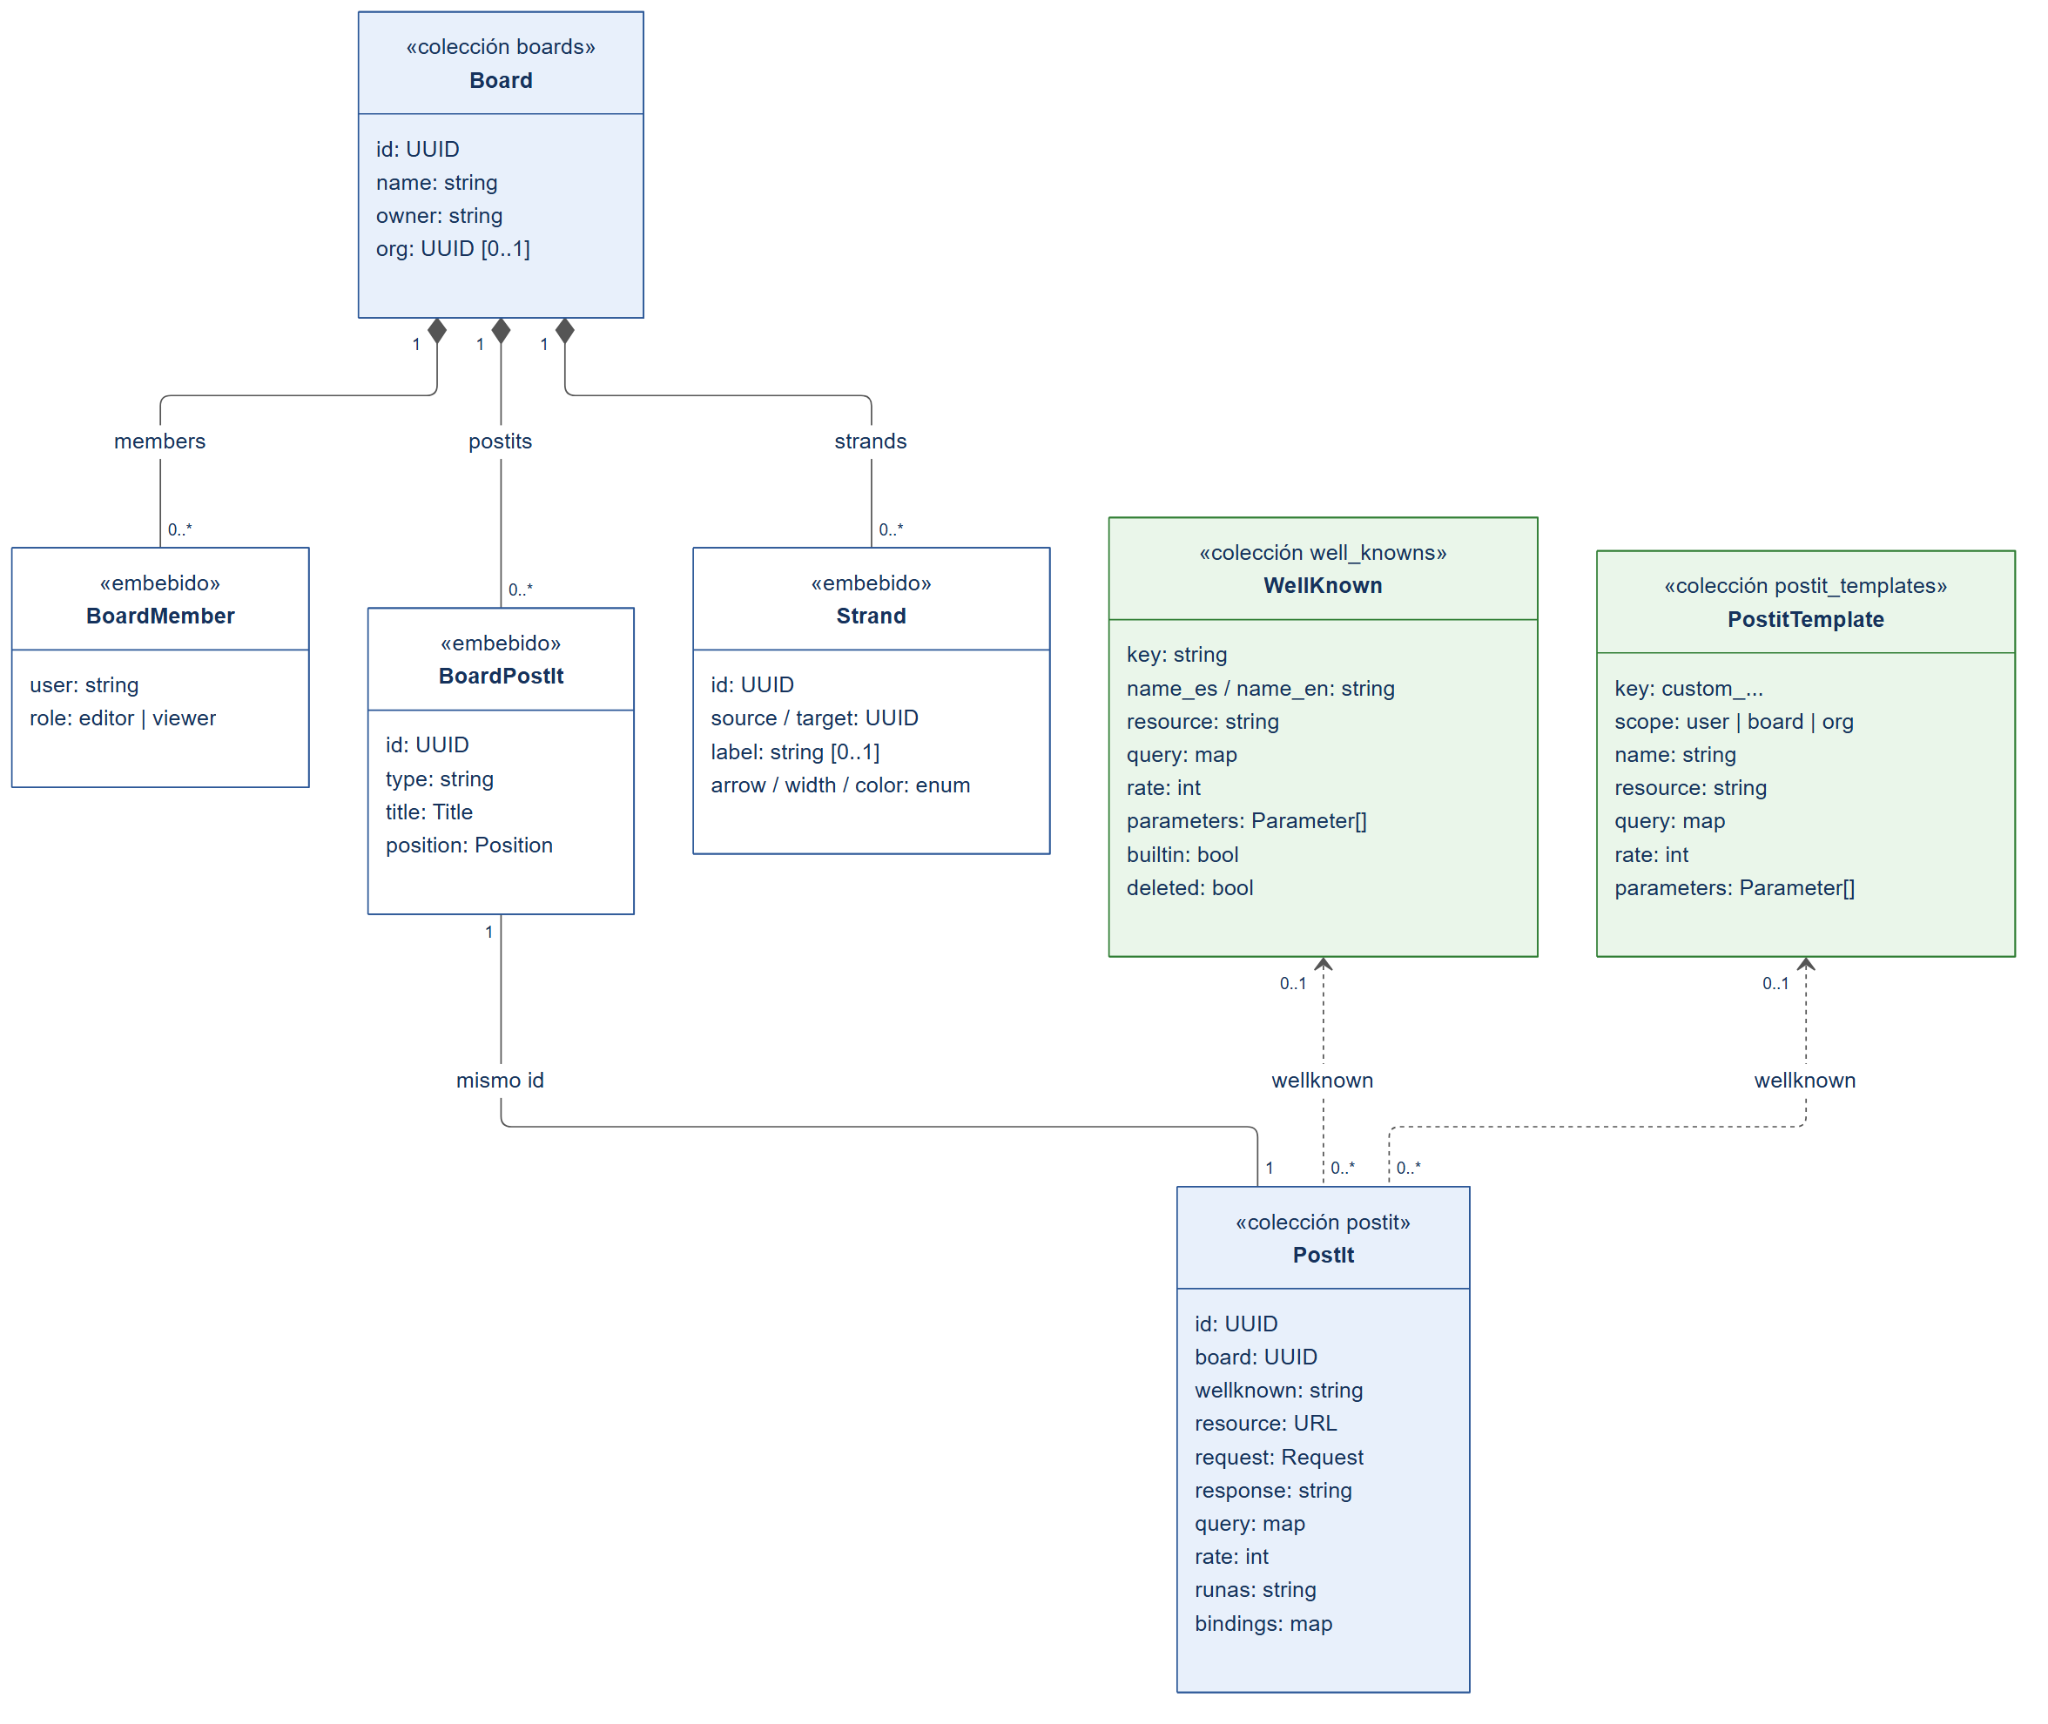
\includegraphics[width=0.95\textwidth]{figuras/fig15.png}
  \caption{Modelo de tableros y tarjetas}
  \label{fig:modelo_tableros_tarjetas}
\end{figure}

\subsection{Identidad y Organizaciones}
El área de identidad se detalla en la Figura~\ref{fig:modelo_identidad}, en la cual cada usuario tiene una o más identidades (contraseña con hash argon2id o cuenta de Google) y puede crear tokens personales, de los que solo se guarda el hash. Las organizaciones listan a sus miembros con rol de administrador o miembro, y los grupos tienen un dueño, una lista de miembros y pueden pertenecer a una organización.

\begin{figure}[H]
  \centering
  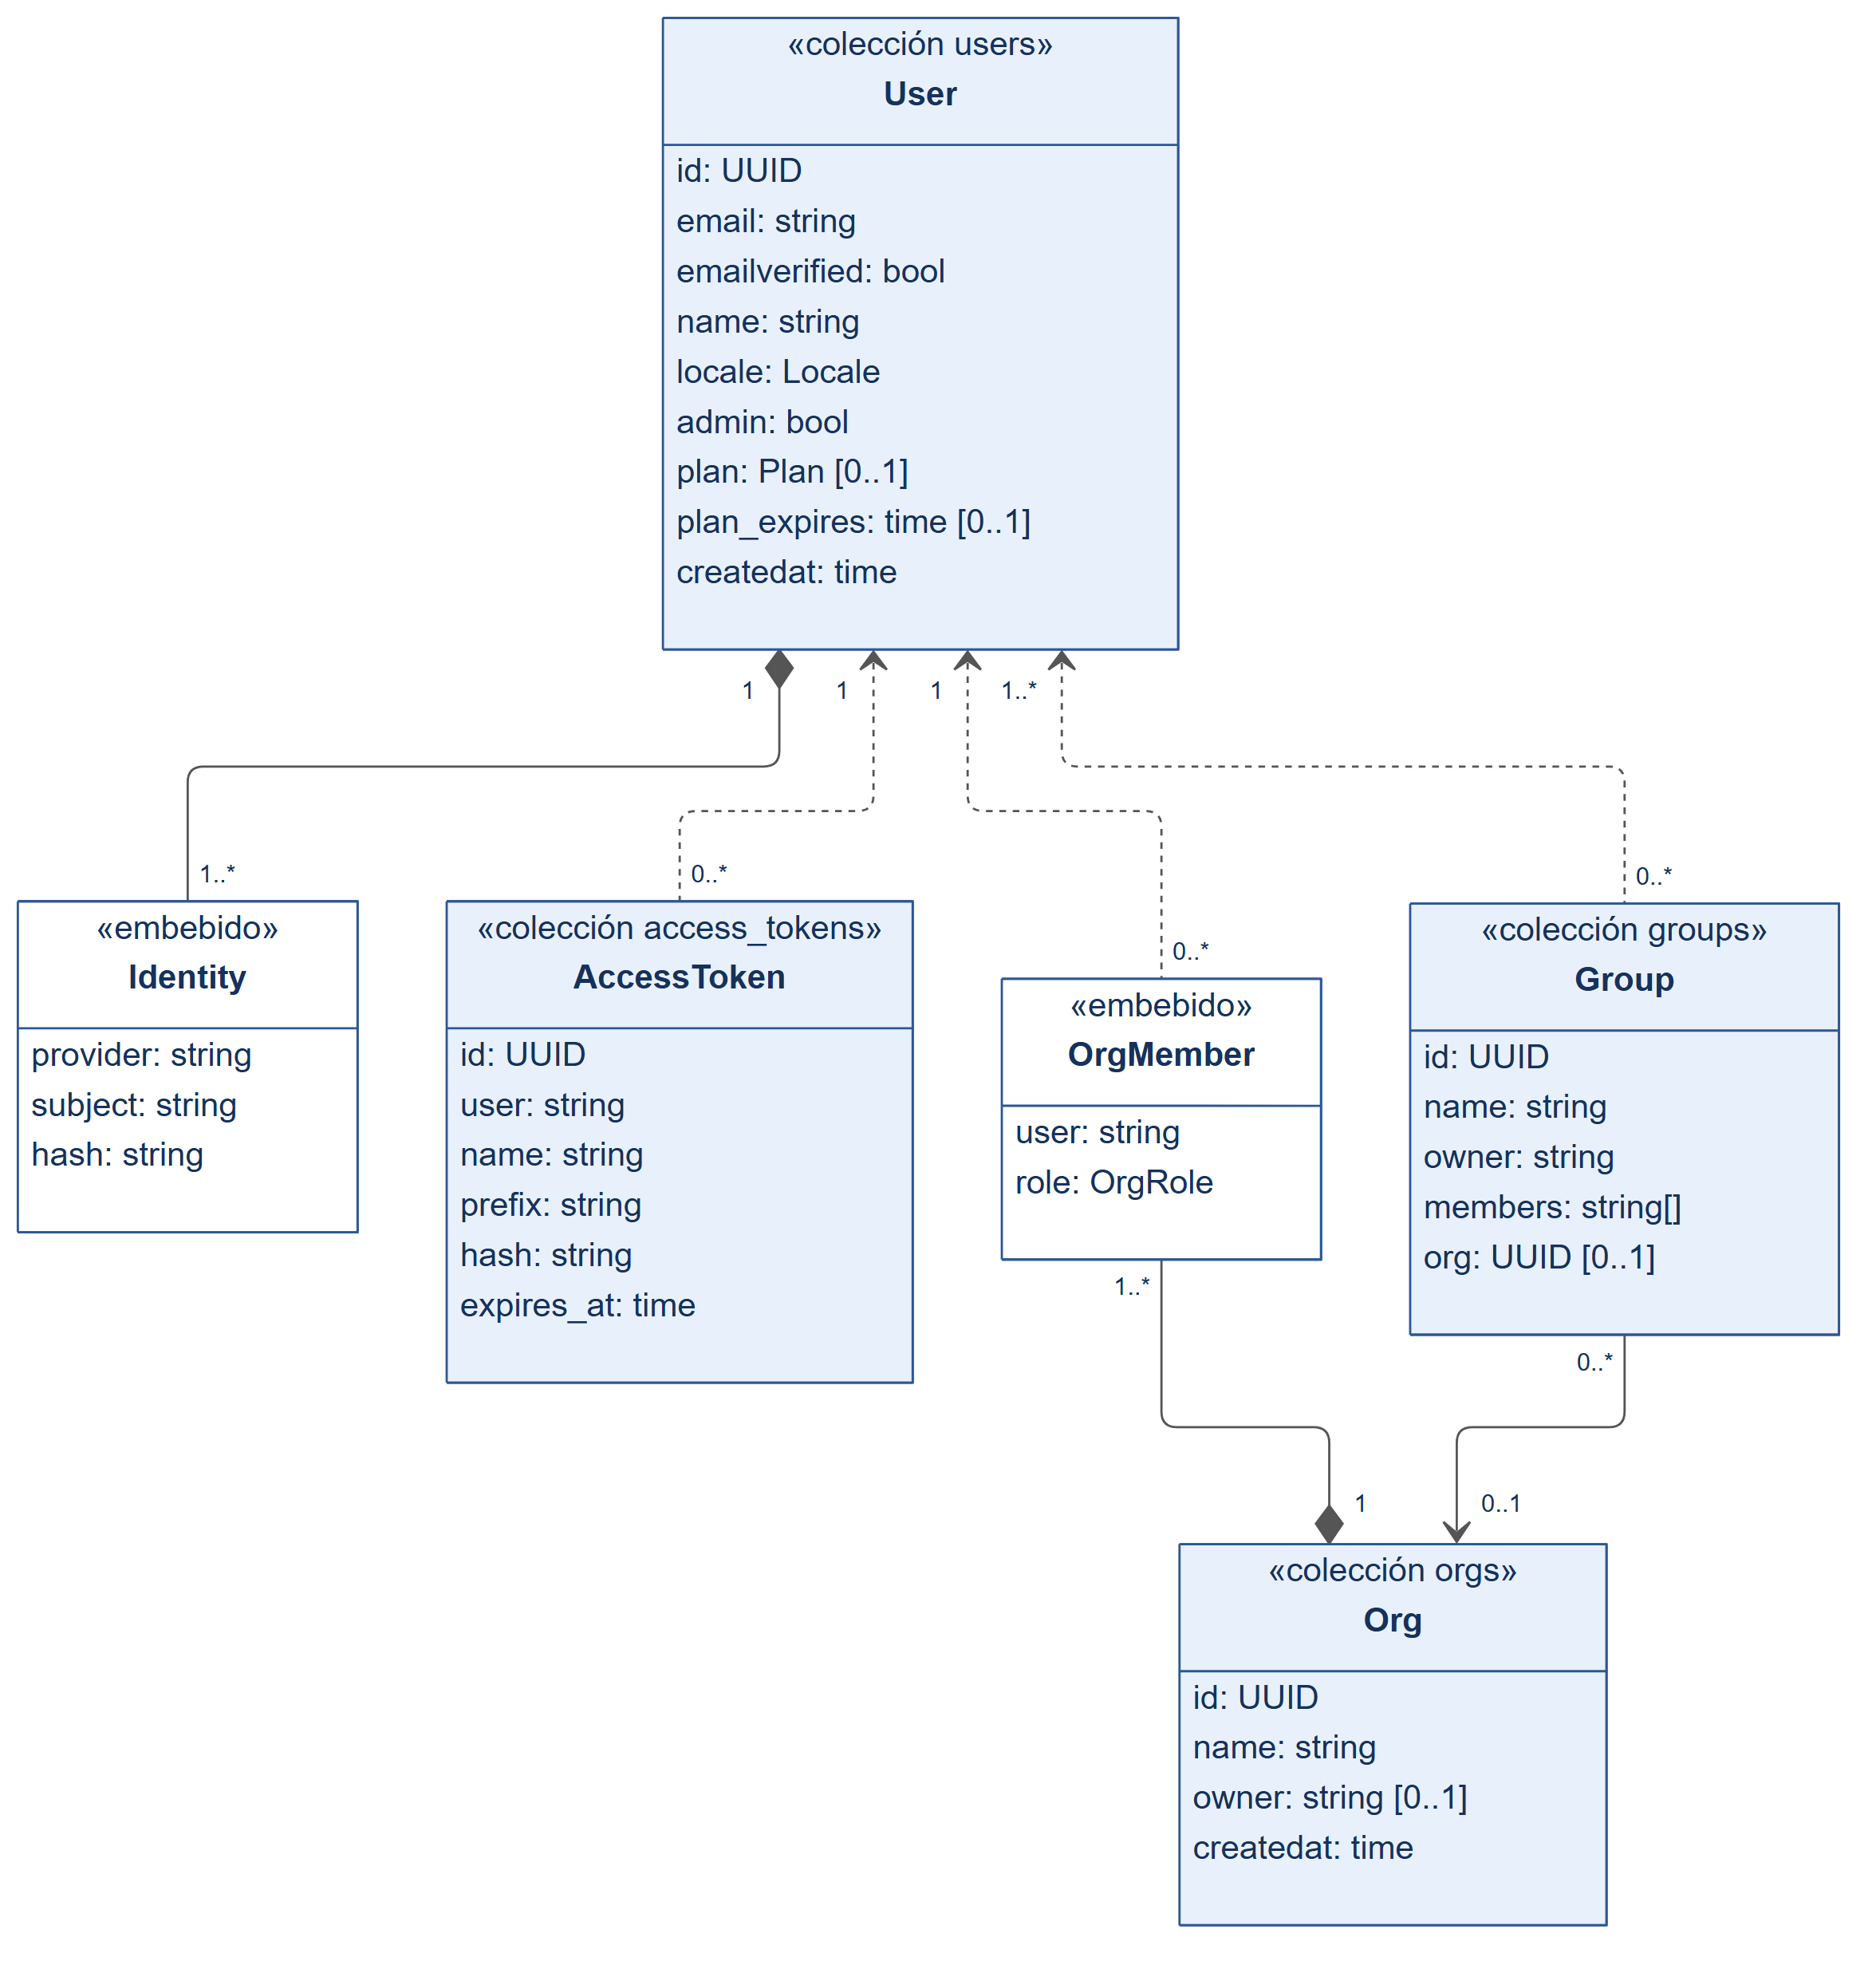
\includegraphics[width=0.92\textwidth]{figuras/fig16.png}
  \caption{Modelo de identidad y organizaciones}
  \label{fig:modelo_identidad}
\end{figure}

\subsection{Bóveda de secretos}
La Figura~\ref{fig:modelo_boveda} muestra el área de la bóveda, en la cual cada tarjeta referencia sus credenciales por ámbito y nombre (\texttt{SecretRef}), sin copiar su valor. Cada secreto se cifra con AES-GCM usando la clave de datos de su ámbito (\texttt{DataKey}), que a su vez se guarda envuelta por la clave maestra versionada, y puede compartirse mediante permisos (\texttt{Grant}) dirigidos a un usuario, un grupo o un tablero.

\begin{figure}[H]
  \centering
  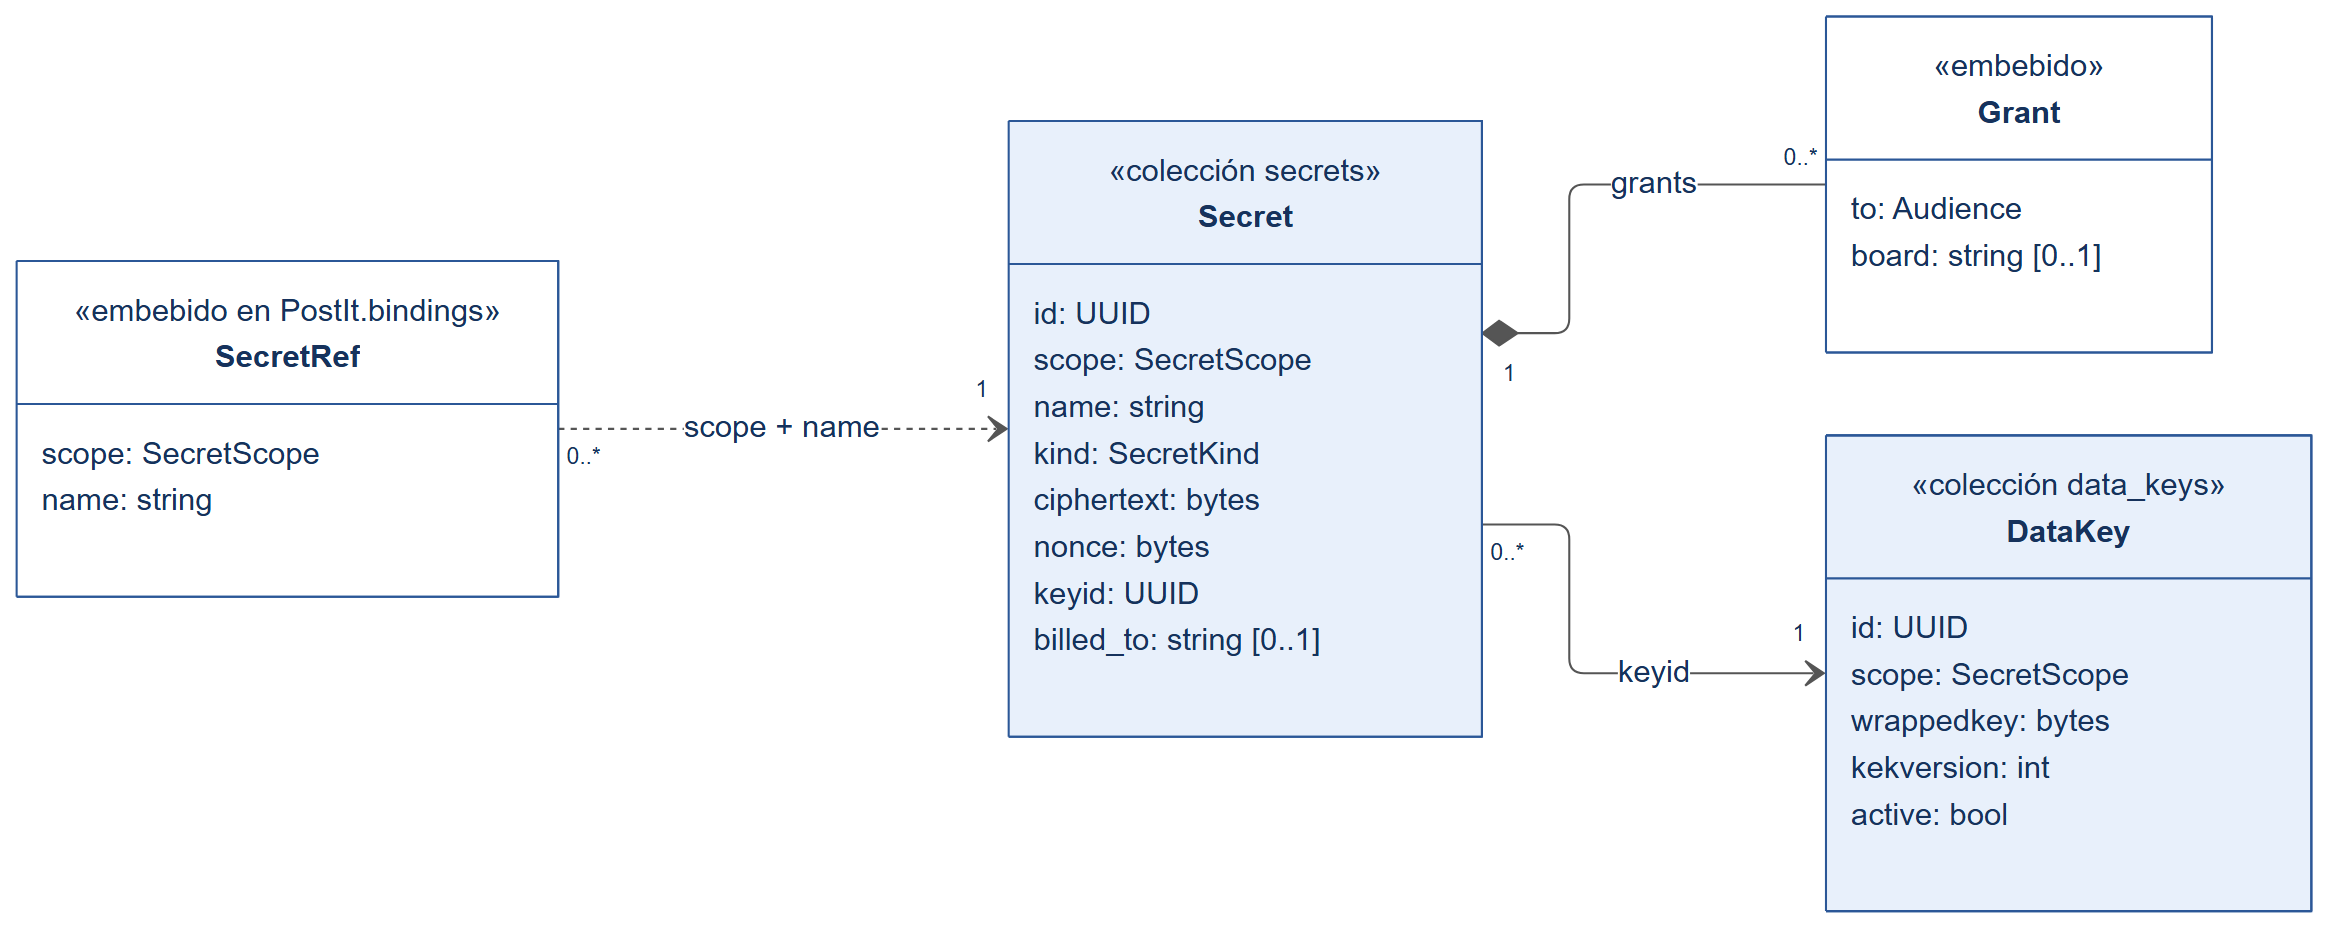
\includegraphics[width=0.95\textwidth]{figuras/fig17.png}
  \caption{Modelo de la bóveda de secretos}
  \label{fig:modelo_boveda}
\end{figure}

\subsection{Planes y suscripciones}
Por último, cada usuario tiene un plan (\texttt{free}, \texttt{pro} o \texttt{max}) con una fecha de vencimiento opcional, y puede tener suscripciones de Mercado Pago que lo mantienen vigente. Los límites de cada plan forman una única tabla (\texttt{Limits}). Cada recurso limitado se factura a un usuario: un tablero a su dueño o al pagador de su organización (\texttt{Org.owner}), y un secreto al usuario indicado en \texttt{billed\_to}. La combinación de pagador, plan y límites que aplica a un recurso se representa con \texttt{Entitlement}. La Figura~\ref{fig:modelo_planes} muestra estas relaciones.

\begin{figure}[H]
  \centering
  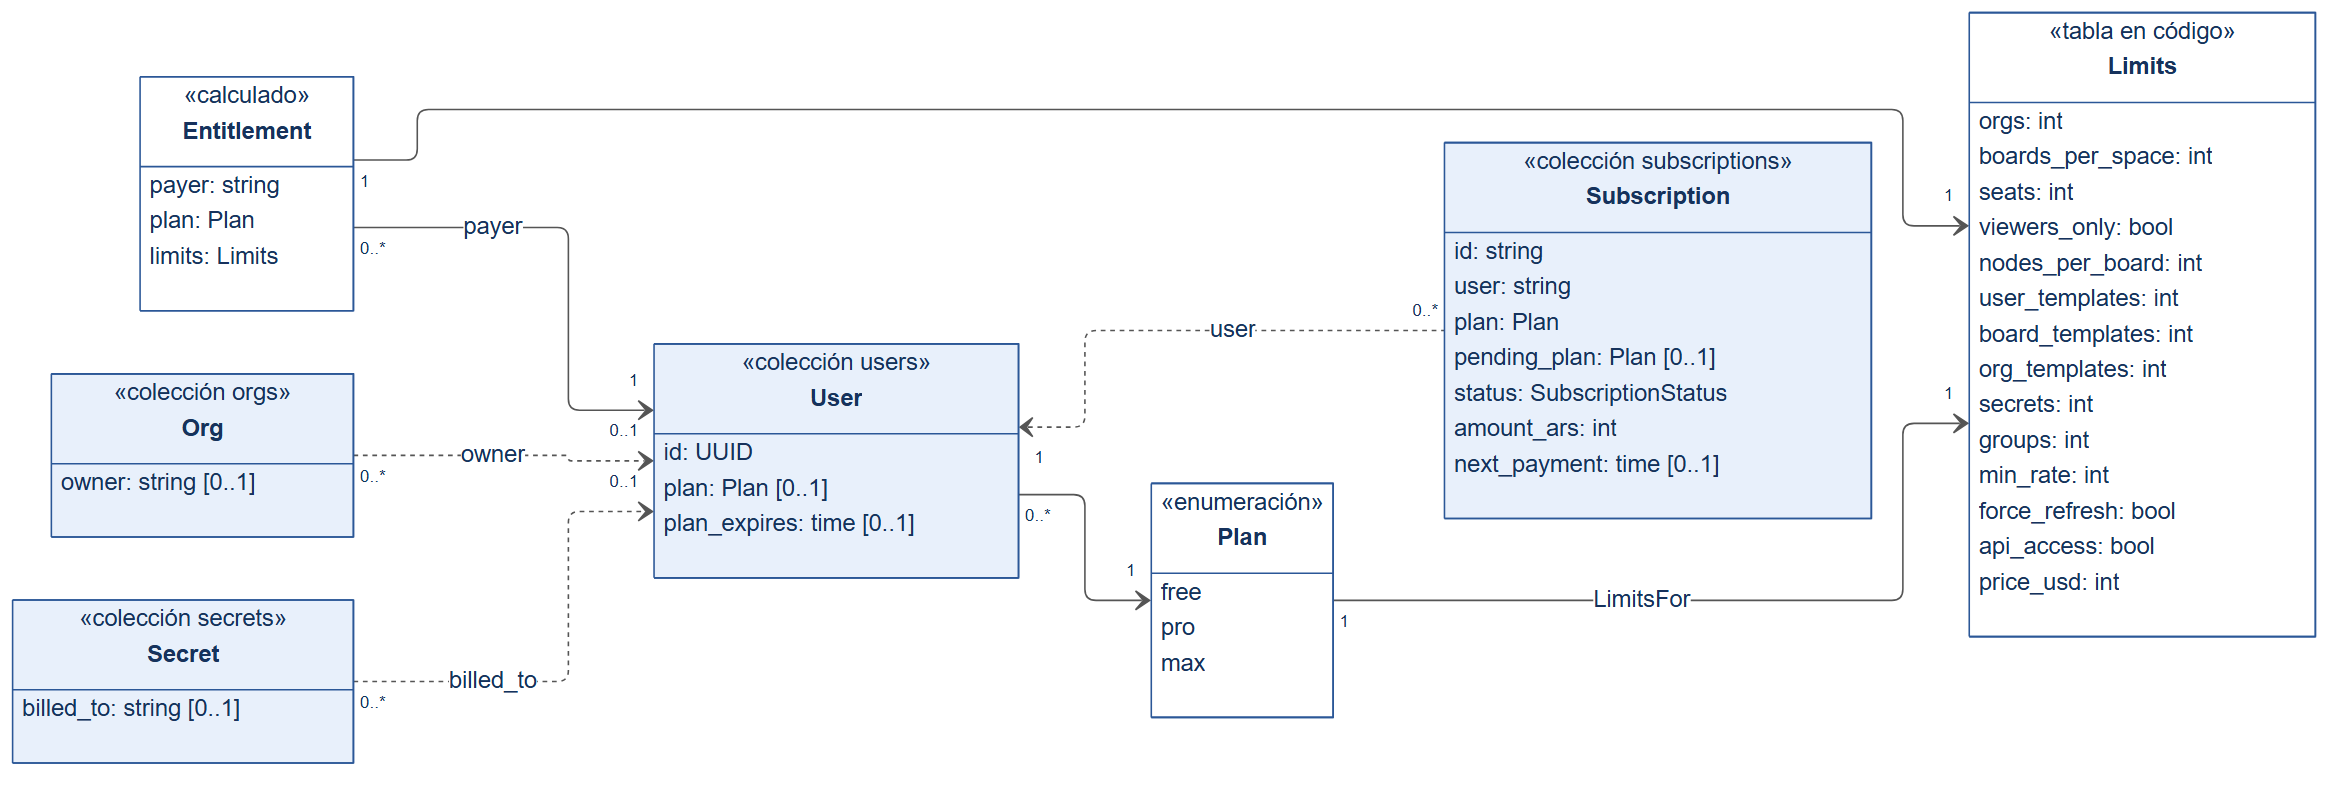
\includegraphics[width=\textwidth]{figuras/fig40.png}
  \caption{Modelo de planes y suscripciones}
  \label{fig:modelo_planes}
\end{figure}

\section{Descripción de sistemas, servicios y plataformas}
A continuación se describe cada componente del sistema, su stack tecnológico, su responsabilidad y la justificación de la elección. Los componentes marcados como planificados forman parte del alcance del proyecto pero no están implementados en el incremento actual.

\begingroup
\footnotesize
\setlength{\tabcolsep}{4.5pt}
\renewcommand{\arraystretch}{1.35}
\rowcolors{2}{gray!7}{white}
\begin{longtable}{
  >{\bfseries\raggedright\arraybackslash}p{\dimexpr 0.16\textwidth - 2\tabcolsep\relax}
  >{\raggedright\arraybackslash}p{\dimexpr 0.24\textwidth - 2\tabcolsep\relax}
  >{\raggedright\arraybackslash}p{\dimexpr 0.30\textwidth - 2\tabcolsep\relax}
  >{\raggedright\arraybackslash}p{\dimexpr 0.30\textwidth - 2\tabcolsep\relax}
}
  \toprule
  \rowcolor{gray!18}
  \textbf{Componente} & \textbf{Tecnología} & \textbf{Responsabilidad} & \textbf{Justificación} \\
  \midrule
  \endfirsthead
  \toprule
  \rowcolor{gray!18}
  \textbf{Componente} & \textbf{Tecnología} & \textbf{Responsabilidad} & \textbf{Justificación} \\
  \midrule
  \endhead
  \midrule
  \rowcolor{white}
  \multicolumn{4}{r}{\textit{\scriptsize Continúa en la página siguiente...}} \\
  \endfoot
  \bottomrule
  \caption{Descripción de componente, la tecnología y la justificación}
  \label{tab:componentes_stack}
  \endlastfoot
  Frontend (SPA) & SvelteKit 2.63 + Svelte 5.56 \cite{svelte_docs}, TailwindCSS 4.3 \cite{tailwind_docs}, TypeScript 6.0 \cite{typescript_docs}, Vite 8.0 \cite{vite_docs}, XyFlow 1.6 \cite{xyflow_docs} & Renderizado del tablero tipo lienzo, manipulación de tarjetas e hilos, edición de configuración y polling de datos a través de la API. & Bundle final pequeño y SSR/SSG opcional, ideal para una interfaz altamente interactiva. Svelte 5 (runes) simplifica el estado reactivo del canvas. \\
  API REST (Backend) & Go 1.27.1 + Gin 1.12 \cite{gin_docs} & Exponer los endpoints bajo \texttt{/api/v1} (auth, users, tokens, boards, post-its, well-knowns, postit-templates, groups, orgs, secrets, billing, system); orquestar autenticación, autorización, persistencia, caché y ejecución de integraciones. & Go aporta concurrencia sencilla (goroutines), tipado estático y binarios pequeños para Docker. Gin se eligió por madurez, middleware y bajo overhead. \\
  Motor de integraciones (Executer) & Go + \texttt{net/http} + \texttt{itchyny/gojq} 0.12 \cite{gojq_docs} + \texttt{PuerkitoBio/goquery} 1.12 \cite{goquery_docs} & Resolver parámetros, ejecutar la petición HTTP, parsear el JSON o HTML y aplicar una expresión jq o jquery para extraer el subconjunto que la tarjeta muestra. & \texttt{gojq} y \texttt{goquery} permiten describir la proyección de datos con sintaxis declarativa estándar, evitando código ad-hoc por integración. Corre con límites (10s y 2MB por petición, hasta 3 redirecciones, 250ms por query). \\
  Base de datos principal & MongoDB 8 \cite{mongodb_docs}, replica set de un nodo & Persistencia de usuarios, tableros, tarjetas, hilos, organizaciones, grupos, la bóveda de secretos y sus claves, tokens personales, el catálogo de integraciones, las plantillas de tarjeta y las suscripciones (11 colecciones, Tabla~\ref{tab:col_boards} y siguientes). & El dominio es naturalmente documental: cada post-it tiene un esquema variable según su integración. Un store relacional implicaría JOINs y normalizaciones sin valor agregado. \\
  Caché de resultados & Redis 7.4 \cite{redis_docs} & Cachear el último resultado de cada post-it, almacenar las sesiones de refresco, los límites de tasa, los locks distribuidos, los handshakes OAuth2 y la presencia por tablero. & TTL nativo por clave que mapea al modelo de tarjeta con su propio refresh rate. Sus operaciones atómicas sirven además para los límites de tasa, los locks distribuidos y la presencia por tablero. \\
  Reverse proxy / ALB & Nginx \cite{nginx_docs} (\texttt{stable-alpine}) & Terminación HTTP en el puerto 80; ruteo de \texttt{/api/*} al backend, de \texttt{/ws/*} al servicio de tiempo real, de \texttt{/mcp} al servidor MCP y del resto al frontend. & Un único entrypoint público que simplifica CORS al servir front y back desde el mismo origen. \\
  Autenticación & Go: \texttt{argon2id} \cite{rfc9106} 1.0, \texttt{golang-jwt} 5.3 \cite{rfc7519} con EdDSA (Ed25519) \cite{rfc8032}, \texttt{go-oidc} 3.21 \cite{oidc_core} para Google & Registro con verificación de correo, login local y con Google, sesiones con token de acceso de 15 minutos y refresh token rotativo en cookie httpOnly. & Una implementación propia evita depender de un proveedor externo y mantiene el mismo flujo en Docker y en Vercel. \texttt{argon2id} es el algoritmo recomendado por OWASP \cite{owasp_password} para contraseñas. \\
  Correo transaccional & Resend \cite{resend_docs} (\texttt{resend-go} 4.8) + plantillas embebidas & Enviar los correos de verificación de cuenta y recuperación de contraseña en el idioma del destinatario. & API simple y de bajo costo; sin clave configurada los correos se vuelcan al log, lo que simplifica el desarrollo local. \\
  Bóveda de secretos & Go: AES-256-GCM \cite{nist_gcm} con envelope encryption & Almacenar credenciales por ámbito (tablero, miembro, usuario, grupo, sistema), resolverlas al ejecutar una tarjeta y gestionar conexiones OAuth2. & El cifrado por sobre (una clave de datos por ámbito envuelta por una clave maestra versionada) permite rotar claves sin recifrar todos los valores. \\
  Planes y facturación & Go + SDK oficial de Mercado Pago (\texttt{mercadopago/sdk-go} 1.14) \cite{mercadopago_docs} & Definir los límites de cada plan, decidir quién paga cada recurso, rechazar con 402 las creaciones que excedan el plan y cobrar las suscripciones mensuales, sincronizándolas mediante webhooks. & Una única tabla de límites en el código evita reglas dispersas. Si no hay credenciales configuradas, la facturación se apaga sin afectar el resto del sistema. \\
  Conector MCP & Servidor MCP en Node.js 24 con \texttt{xmcp} 1.7, que consume la API REST del backend & Exponer tableros y tarjetas a clientes MCP (Claude Desktop, IDEs) para RF-10 y la fase final del cronograma mediante 11 herramientas que presentan cada tablero como un grafo de memorias del agente. & Reutiliza la API REST ya validada y sus reglas de autorización; el servidor MCP es una segunda fachada sobre los mismos casos de uso y no almacena datos propios. Requiere un plan pago (\texttt{api\_access}). \\
  Servicio de tiempo real & Node.js 24 + TypeScript 6.0 + \texttt{socket.io} 4.8 \cite{socketio_docs} & Notificar a cada usuario conectado los cambios de un tablero y mantener la presencia de los participantes. & Los change streams de MongoDB y \texttt{socket.io} permiten propagar cambios sin polling. Separarlo del backend aísla las conexiones persistentes de la API stateless. \\
\end{longtable}
\endgroup

% !TEX root = ../main.tex
\chapter{Diseño de Bajo Nivel}

Siguiendo una arquitectura hexagonal, se desarrolló una capa de servicios que concentra los casos de uso del dominio y depende únicamente de puertos definidos como interfaces, mientras que los adaptadores de infraestructura proveen las implementaciones concretas de esos puertos. Esta separación es la que permite cumplir el RNF-04, ya que habilita incorporar nuevas integraciones o reemplazar tecnologías subyacentes sin alterar la lógica de negocio.

La Figura~\ref{fig:capas_backend} esquematiza la organización en capas del backend y la interacción entre sus componentes. Cada solicitud HTTP atraviesa primero los middlewares de autenticación y autorización. Luego, el controlador del recurso se encarga de interpretar la solicitud y construir la respuesta correspondiente, delegando la ejecución del caso de uso al servicio.

Los servicios dependen únicamente de las interfaces definidas en el paquete \texttt{infrastructure}, que actúan como puertos de la arquitectura. Por su parte, los adaptadores del paquete \texttt{ports} implementan dichas interfaces mediante tecnologías concretas, como MongoDB, Redis, JWT, Argon2id, OIDC, mecanismos de cifrado, OAuth2, el cliente HTTP seguro, el motor de integraciones, el servicio de correo y la pasarela de pagos de Mercado Pago. Finalmente, los tipos de dominio definidos en el paquete \texttt{models} son compartidos por las distintas capas del backend.

\begin{figure}[H]
  \centering
  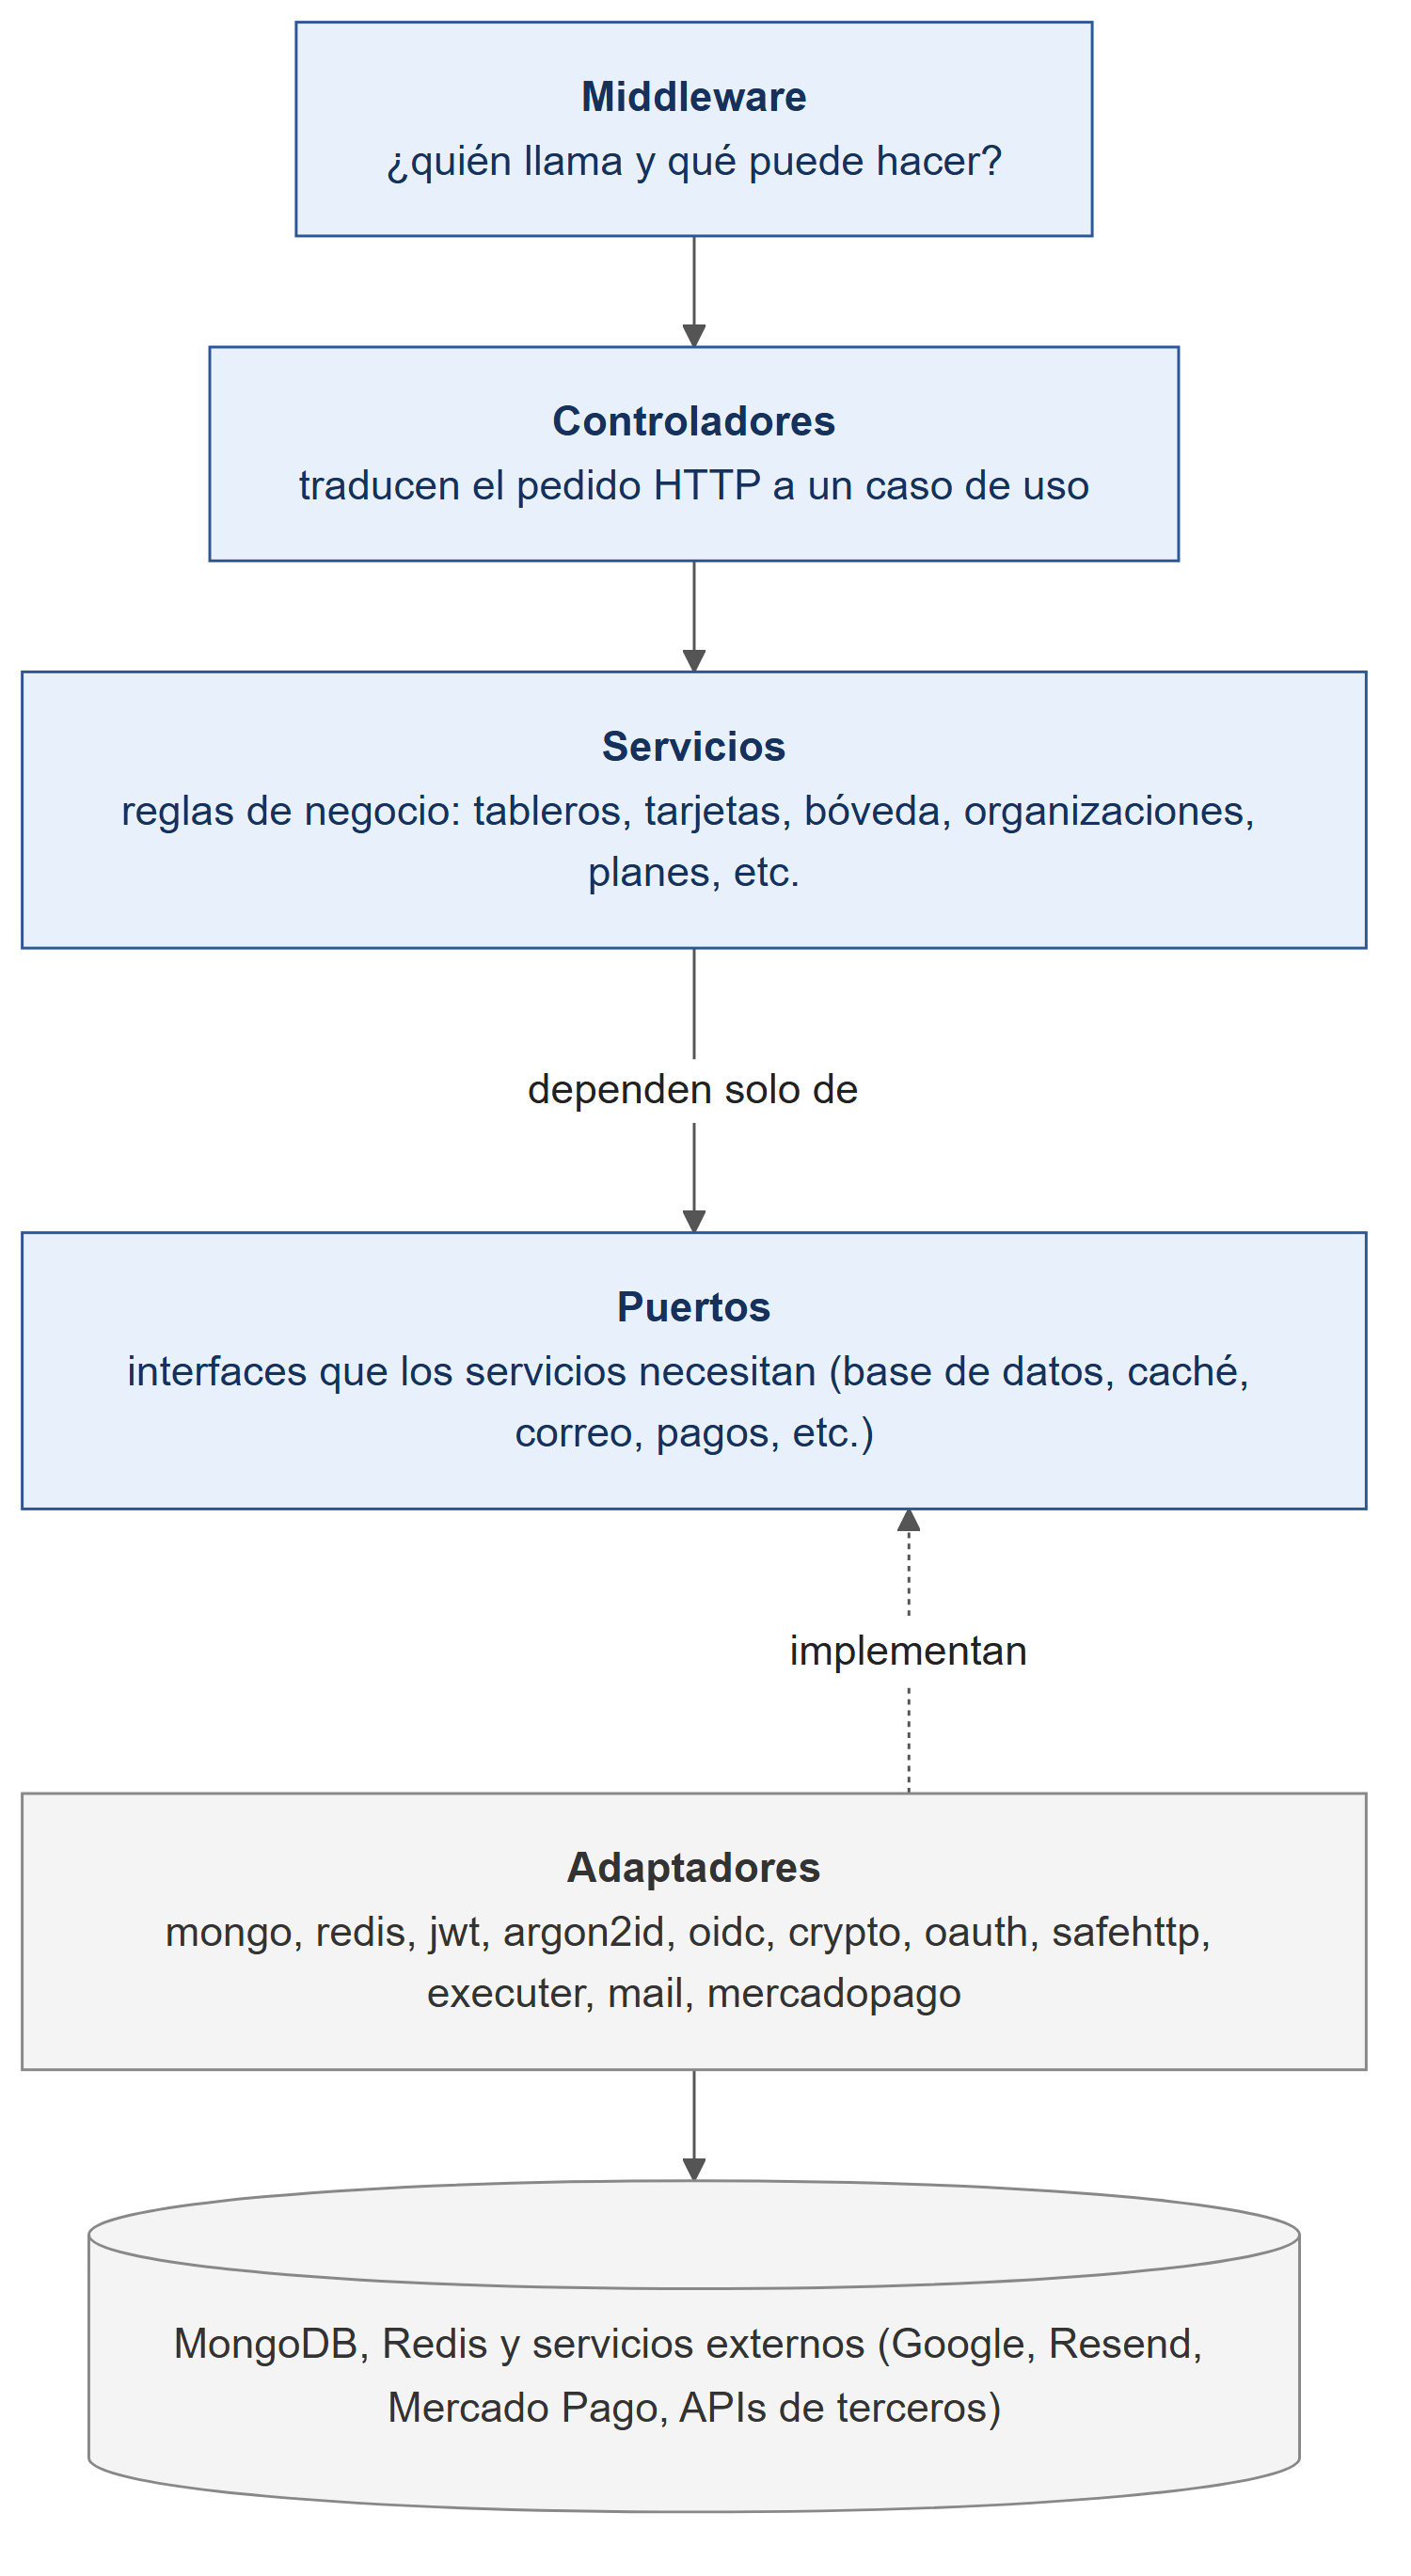
\includegraphics[width=0.65\textwidth]{figuras/fig18.png}
  \caption{Diagrama de capas del backend}
  \label{fig:capas_backend}
\end{figure}

A continuación se describen los componentes que ya se encuentran implementados en el incremento actual, indicando para cada uno su responsabilidad, su estructura en capas y los requisitos funcionales que cubre.

\section{Autenticación y Usuarios}
Este componente, materializado en los paquetes \texttt{auth} y \texttt{users}, es responsable del registro, el inicio de sesión local y federado, y la gestión del perfil propio, cubriendo los requisitos RF-01, RF-02 y RNF-02. Al igual que el resto de los componentes, se divide en controlador, servicio y adaptadores: argon2id para el hash de contraseñas, un keyring EdDSA para firmar los tokens, un cliente OIDC para Google y Redis para las sesiones y los límites de tasa.

La Figura~\ref{fig:clases_auth} presenta el diagrama de clases del componente. Los tres servicios dependen únicamente de interfaces: el almacenamiento de usuarios y sesiones, el hash de contraseñas, la firma de tokens, los límites de tasa, el envío de correos y el proveedor de identidad de Google, cuyas implementaciones concretas se encuentran en el paquete \texttt{ports}.

\begin{figure}[H]
  \centering
  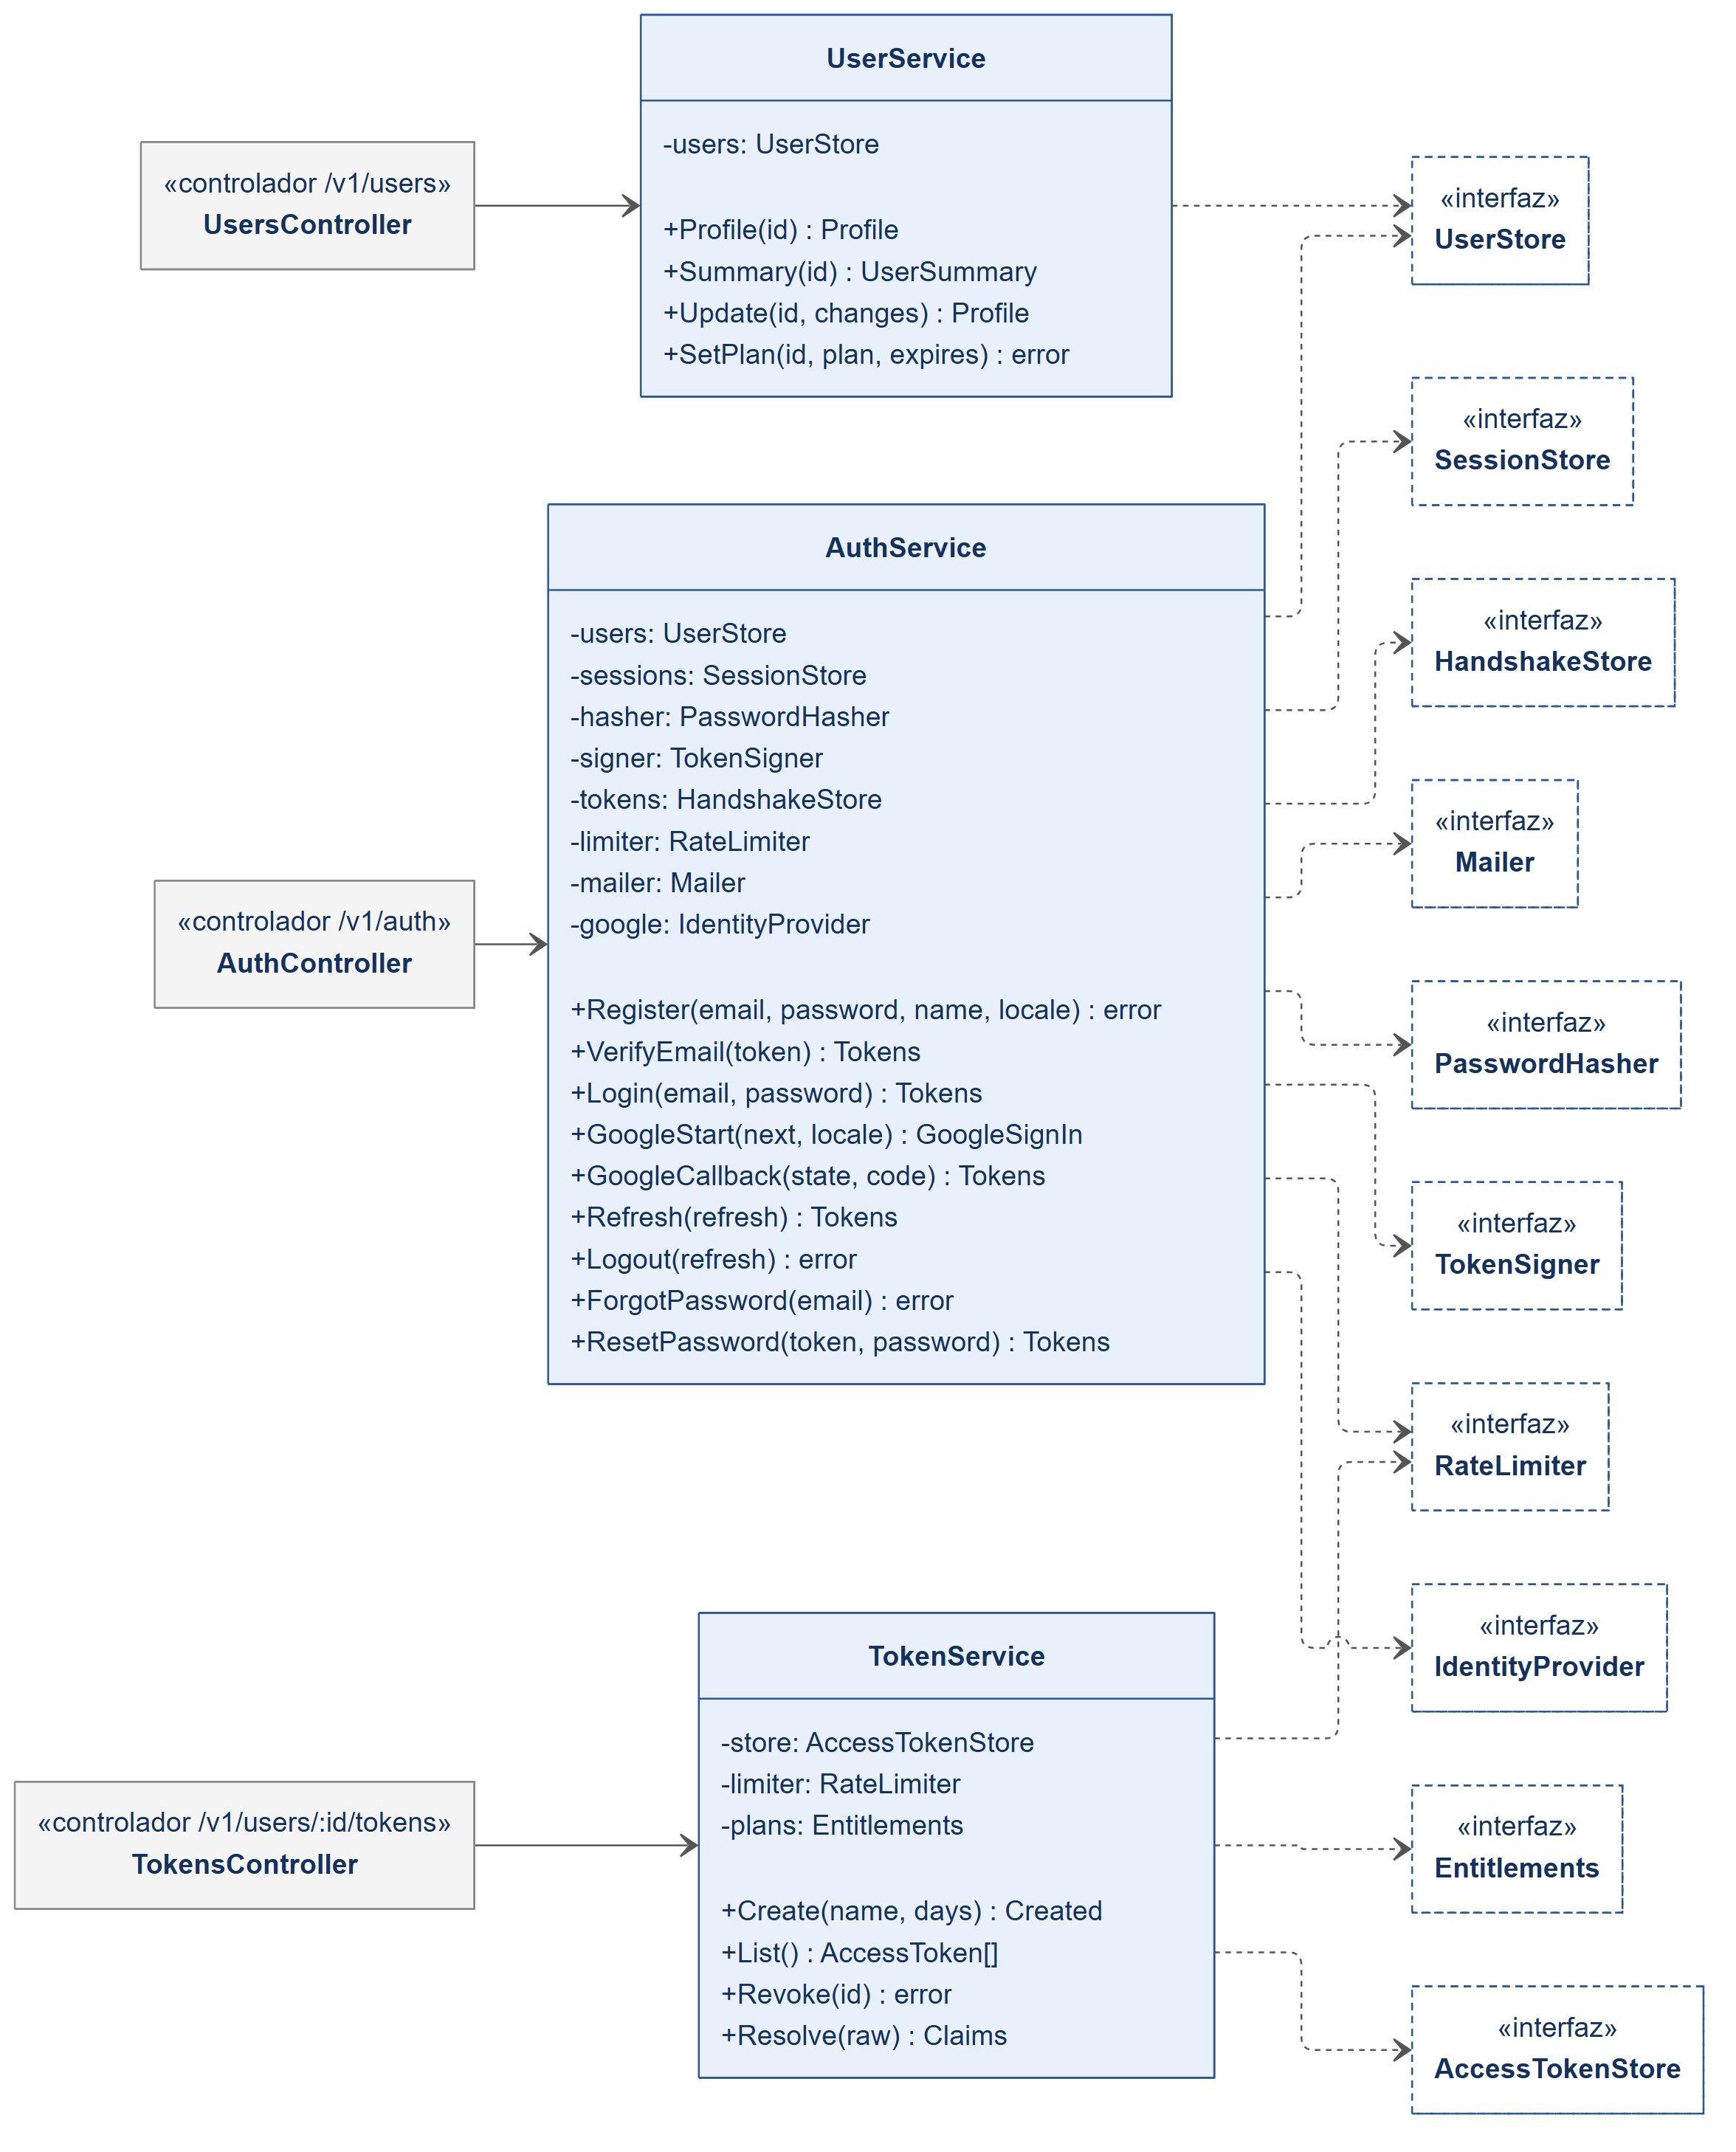
\includegraphics[width=0.92\textwidth]{figuras/fig19.png}
  \caption{Diagrama de clases de autenticación y usuarios}
  \label{fig:clases_auth}
\end{figure}

Una sesión se compone de un token de acceso JWT de quince minutos, que el frontend conserva únicamente en memoria y envía como \texttt{Authorization: Bearer}, y de un refresh token rotativo almacenado en Redis y transportado en la cookie httpOnly \texttt{tiu\_refresh}. Cada renovación emite un nuevo refresh token; si uno ya utilizado vuelve a presentarse pasado un margen de diez segundos, se revoca la familia completa de sesiones, lo que mitiga el robo de tokens. Las rutas que leen la cookie rechazan además las peticiones cross-site mediante el header \texttt{Sec-Fetch-Site}.

En la siguiente tabla se resumen los endpoints implementados para el servicio.

\begin{tablaendpoints}{Endpoints de Auth y Users}{tab:endpoints_auth}
  POST & /auth/register & Registrar una cuenta y enviar el correo de verificación. \\
  POST & /auth/verify-email & Verificar el correo con el token recibido. \\
  POST & /auth/login & Iniciar sesión con correo y contraseña. \\
  POST & /auth/refresh & Renovar la sesión a partir de la cookie de refresco. \\
  POST & /auth/logout & Cerrar la sesión y revocar el refresh token. \\
  POST & /auth/password/forgot & Solicitar el correo de recuperación de contraseña. \\
  POST & /auth/password/reset & Restablecer la contraseña con el token recibido. \\
  GET & /auth/google/start & Iniciar el flujo de inicio de sesión con Google. \\
  POST & /auth/google/callback & Completar el inicio de sesión con Google. \\
  GET & /users/\{id\} & Obtener el perfil propio, con su plan y sus límites. \\
  PATCH & /users/\{id\} & Editar el perfil propio (nombre, idioma). \\
  GET & /users/\{id\}/tokens & Listar los tokens personales propios (sin su valor). \\
  POST & /users/\{id\}/tokens & Crear un token personal (7, 15 o 30 días); su valor se muestra una única vez. \\
  DELETE & /users/\{id\}/tokens/\{token\} & Revocar un token personal. \\
  PUT & /system/users/\{id\}/plan & Asignar un plan sin pago (solo administradores). \\
\end{tablaendpoints}

Los endpoints de login, registro y recuperación aplican límites de tasa tanto por dirección de origen como por cuenta, respondiendo 429 al superarlos, lo que dificulta los ataques de fuerza bruta y el envío masivo de correos.

Los tokens personales, en el paquete \texttt{tokens}, permiten que herramientas externas como el servidor MCP actúen en nombre de un usuario. El verificador de tokens envuelve al de los JWT, de modo que el middleware de autenticación acepta ambos: un token personal se reconoce por su prefijo \texttt{tiu\_pat\_}, se busca por su hash SHA-256 y produce un principal marcado como token, que nunca es administrador. Un segundo middleware limita ese principal a una lista explícita de rutas (lectura de tableros, tarjetas, organizaciones, el perfil y el catálogo, y creación, edición y eliminación de tableros, tarjetas e hilos), por lo que toda ruta nueva queda cerrada a los tokens hasta que se la habilite. Cada usuario puede tener hasta diez tokens activos, la creación está limitada a diez por hora, y tanto la creación como cada uso verifican que el plan del usuario incluya acceso por API.

\section{Control de acceso y organizaciones}
El control de acceso se concentra en el paquete \texttt{access}, que constituye el único lugar del sistema donde se decide el rol de un principal sobre un recurso. Los servicios nunca comparan identificadores por su cuenta, sino que consultan al puerto \texttt{infrastructure.Access} y comparan el rol obtenido con el mínimo requerido mediante \texttt{AtLeast}.

Sobre un tablero existen tres roles jerárquicos: \texttt{owner}, \texttt{editor} y \texttt{viewer}. Los viewers pueden leer el tablero, sus miembros y los resultados de las tarjetas; los editors pueden además crear, editar, mover y eliminar tarjetas y dibujar hilos; finalmente, el owner puede también renombrar, eliminar y compartir el tablero. Por debajo del rol que una ruta requiere, el tablero responde 404.

Por su parte, las organizaciones, en el paquete \texttt{orgs}, funcionan como un tenant mínimo con roles \texttt{admin} y \texttt{member}. Un tablero creado dentro de una organización alcanza a todos sus miembros sin necesidad de compartirlo: los admins actúan como owners y los members como viewers, prevaleciendo el mayor entre ese rol y el asignado explícitamente en el tablero. La invariante de que una organización conserve al menos un administrador se garantiza en el propio filtro de MongoDB, evitando condiciones de carrera entre degradaciones concurrentes, y una organización solo puede eliminarse cuando ningún tablero ni grupo la referencia. Cada organización tiene además un pagador, su dueño o en su defecto su primer administrador, cuyo plan determina los límites de la organización y de sus tableros.

Los grupos, en el paquete \texttt{groups}, agrupan usuarios con el propósito principal de compartir secretos. En un grupo perteneciente a una organización, los admins actúan como owners y los members solo lo ven, de modo que los secretos del grupo permanecen restringidos a las personas que este lista.

Las clases que intervienen se muestran en la Figura~\ref{fig:clases_access}. El \texttt{Resolver} implementa el puerto \texttt{Access} que consultan los demás servicios para conocer el rol de un principal, mientras que \texttt{OrgService} y \texttt{GroupService} gestionan los miembros y delegan en el puerto \texttt{ScopePurger} la eliminación de los secretos de quien deja de pertenecer. Ambos servicios consultan además el puerto \texttt{Entitlements} para rechazar, con 402, la creación de organizaciones o grupos y el ingreso de miembros que excedan el plan correspondiente.

\begin{figure}[H]
  \centering
  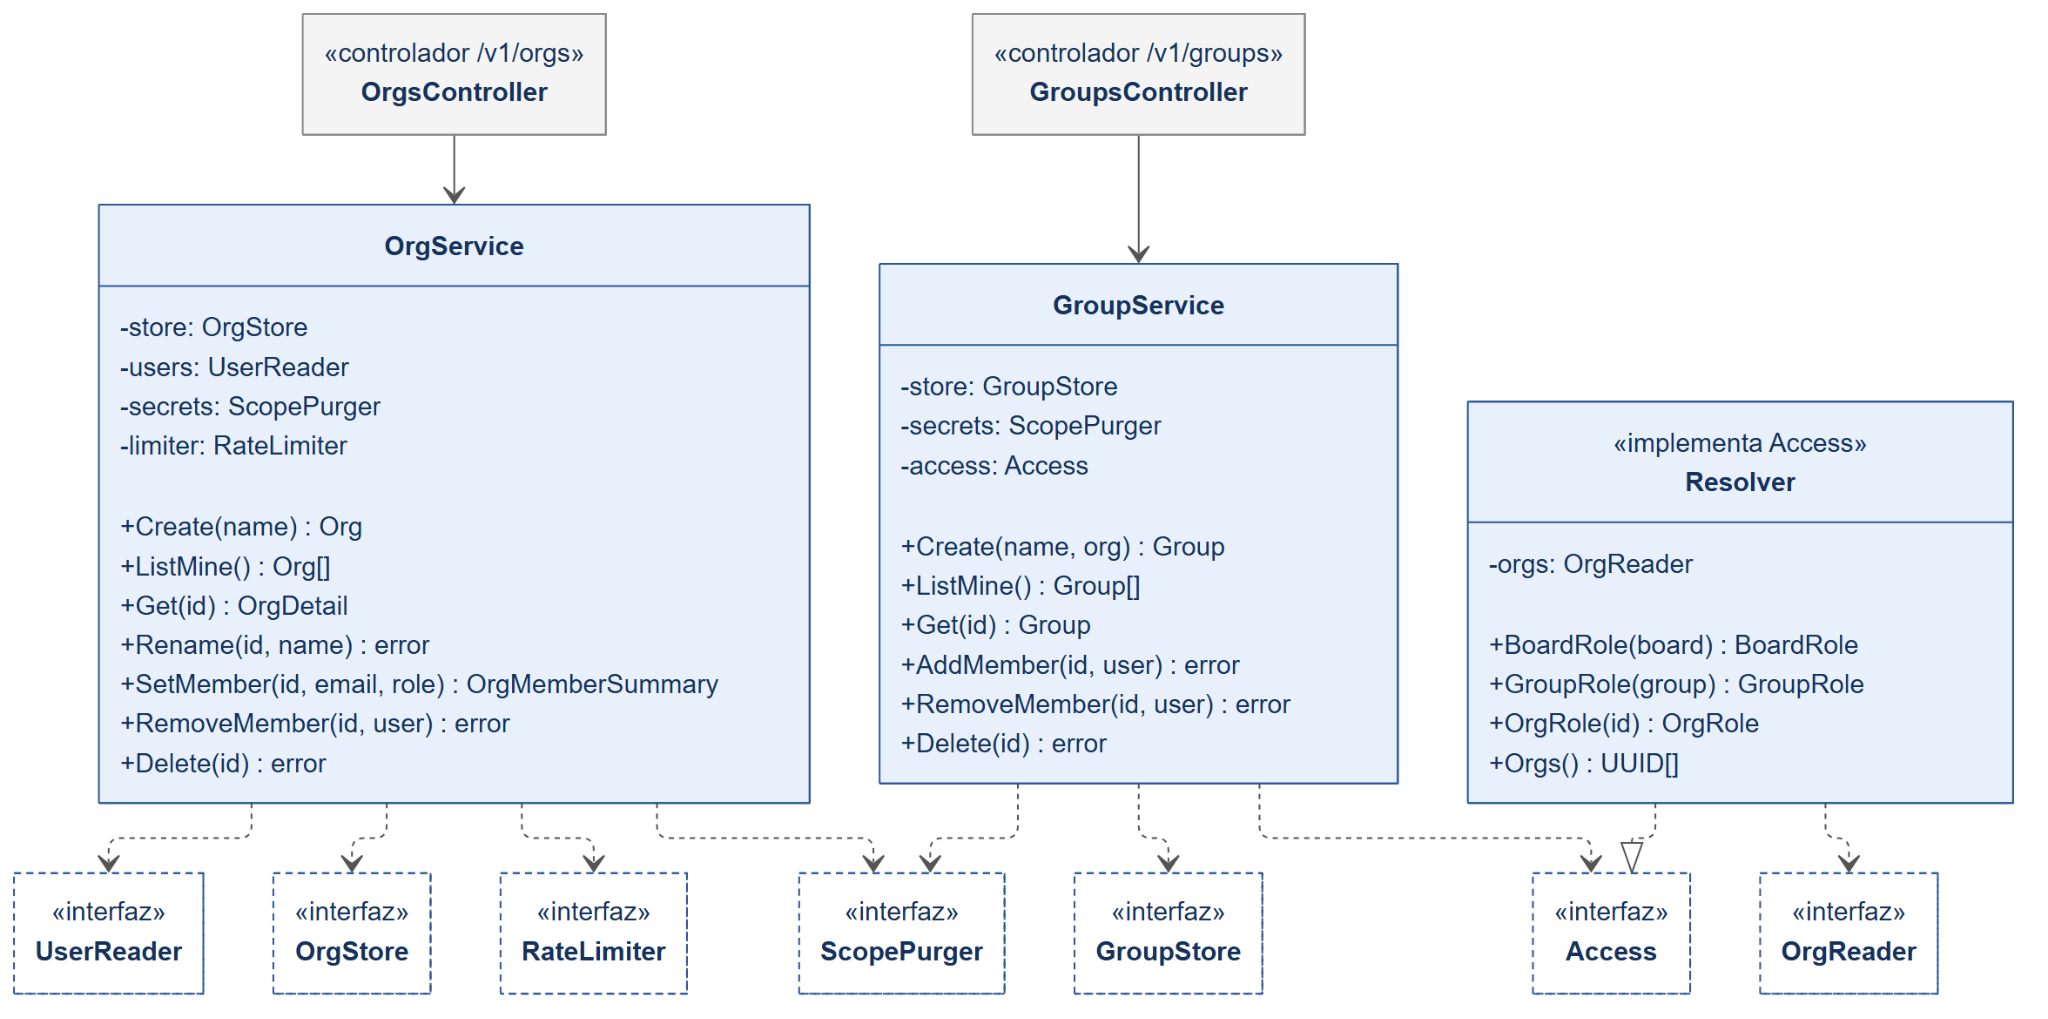
\includegraphics[width=0.95\textwidth]{figuras/fig20.png}
  \caption{Diagrama de clases de control de acceso y organizaciones}
  \label{fig:clases_access}
\end{figure}

\begin{tablaendpoints}{Endpoints de Orgs y Groups}{tab:endpoints_orgs_groups}
  GET & /orgs & Listar las organizaciones del usuario. \\
  POST & /orgs & Crear una organización. \\
  GET & /orgs/\{id\} & Obtener una organización con sus miembros, su plan y su uso. \\
  PATCH & /orgs/\{id\} & Renombrar la organización. \\
  DELETE & /orgs/\{id\} & Eliminar la organización si está vacía. \\
  PUT & /orgs/\{id\}/members & Agregar un miembro por correo o cambiar su rol. \\
  DELETE & /orgs/\{id\}/members/\{user\} & Quitar un miembro o abandonar la organización. \\
  GET & /groups & Listar los grupos del usuario. \\
  POST & /groups & Crear un grupo (opcionalmente dentro de una organización). \\
  GET & /groups/\{id\} & Obtener un grupo. \\
  DELETE & /groups/\{id\} & Eliminar el grupo y purgar sus secretos. \\
  POST/DELETE & /groups/\{id\}/members & Agregar/quitar un miembro. \\
\end{tablaendpoints}

\section{Gestión de Tableros}
Este componente, materializado en el paquete \texttt{boards}, es responsable del CRUD de tableros, de la gestión de miembros por rol y de las conexiones (\texttt{strands}) entre tarjetas, cubriendo los requisitos RF-04 y RF-06. Internamente se divide en tres capas bien diferenciadas.

El controlador, en \texttt{controllers/boards/controllers.go}, expone los endpoints REST bajo \texttt{/v1/boards}. El servicio, en \texttt{services/boards/main.go}, verifica el rol del llamante a través del puerto \texttt{Access}, orquesta las operaciones de dominio y delega la persistencia en el puerto \texttt{infrastructure.Database}, sin acoplarse a ninguna tecnología concreta. Finalmente, el adaptador en \texttt{ports/mongo/mon.go} provee la implementación concreta sobre MongoDB.

Esta estructura se refleja en la Figura~\ref{fig:clases_boards}, donde \texttt{BoardService} depende de los puertos \texttt{Database} y \texttt{Access} para persistir y autorizar, de \texttt{UserReader} para resolver a los miembros por correo, de \texttt{ScopePurger} para purgar sus secretos, de \texttt{RateLimiter} para limitar las invitaciones, de \texttt{OrgReader} para conocer la organización del tablero y de \texttt{Entitlements} para aplicar los límites del plan de quien lo paga.

\begin{figure}[H]
  \centering
  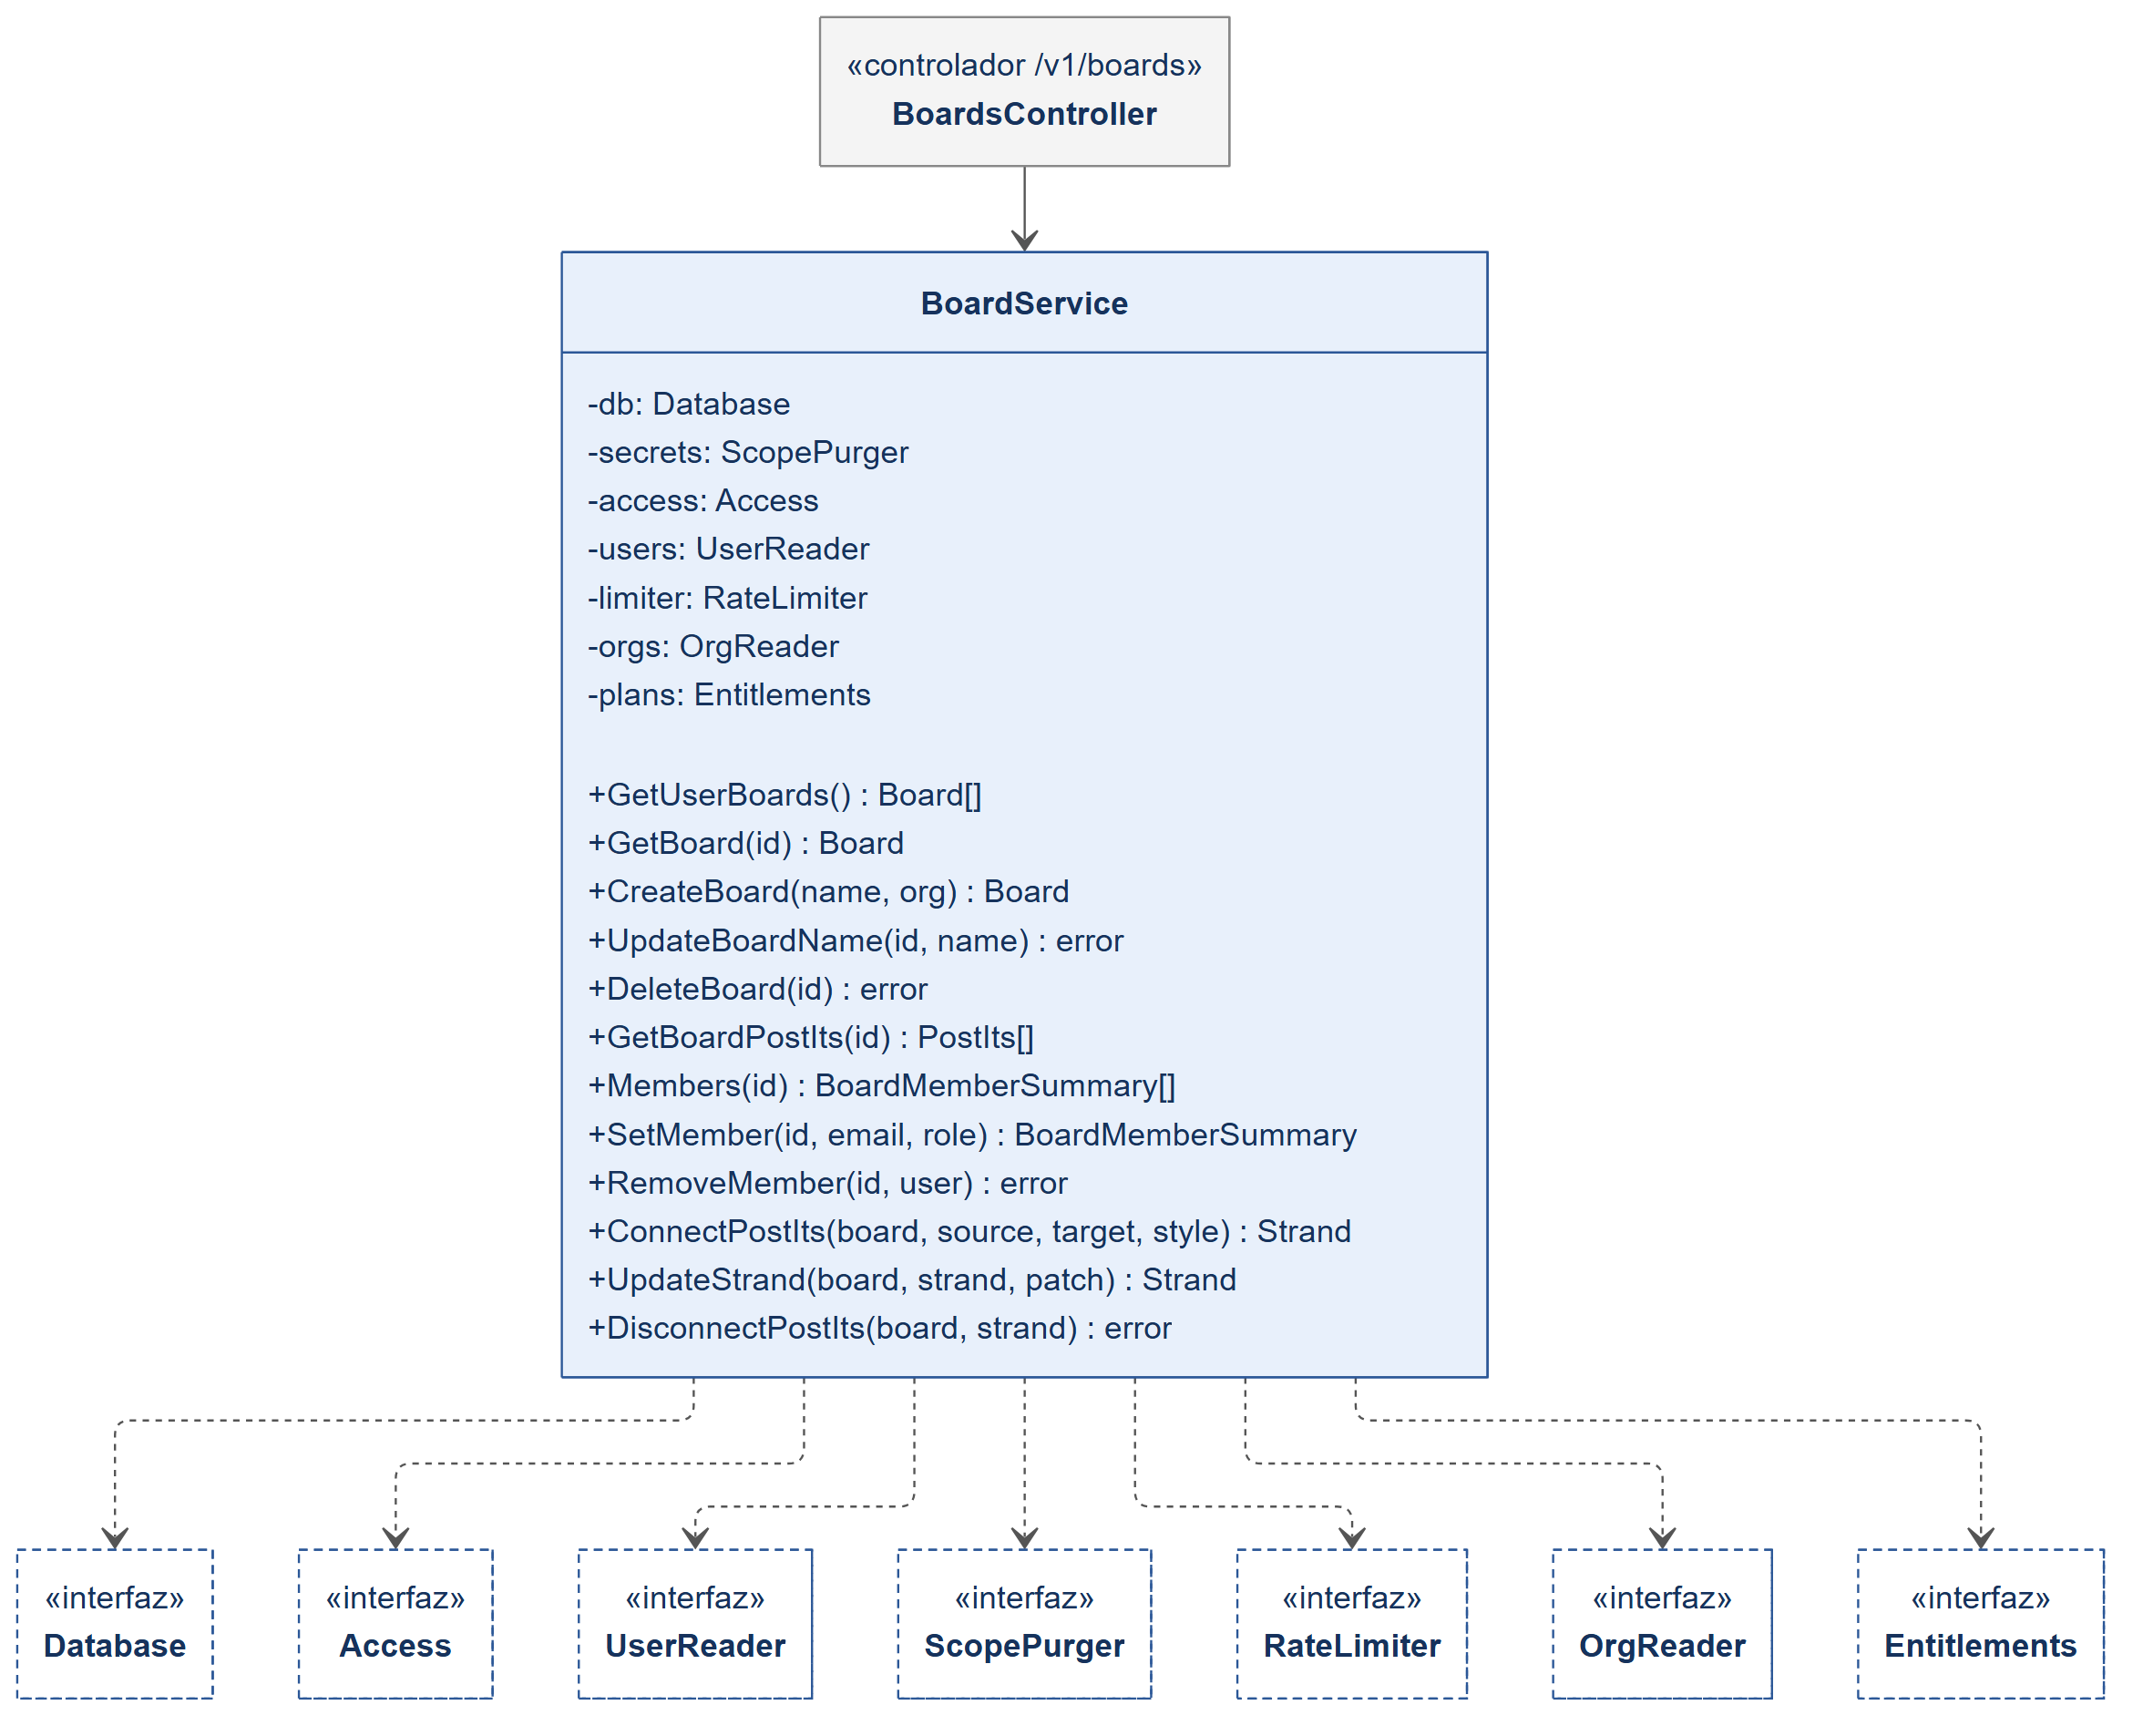
\includegraphics[width=0.82\textwidth]{figuras/fig21.png}
  \caption{Diagrama de clases de gestión de tableros}
  \label{fig:clases_boards}
\end{figure}

En la siguiente tabla se resumen los endpoints implementados para el servicio.

\begin{tablaendpointsrol}{Endpoints de Boards}{tab:endpoints_boards}
  GET & /boards & Listar los tableros propios, compartidos y de las organizaciones del usuario. & — \\
  GET & /boards/\{id\} & Obtener un tablero junto con el rol del llamante. & viewer \\
  POST & /boards & Crear tablero (name, org opcional). & — \\
  DELETE & /boards/\{id\} & Eliminar tablero, sus post-its y purgar sus secretos y claves. & owner \\
  GET & /boards/\{id\}/post-its & Listar post-its asociados. & viewer \\
  PATCH & /boards/\{id\}/name & Renombrar tablero. & owner \\
  GET & /boards/\{id\}/members & Listar los miembros con su rol. & viewer \\
  PUT & /boards/\{id\}/members & Agregar un miembro por correo o cambiar su rol. & owner \\
  DELETE & /boards/\{id\}/members/\{user\} & Quitar un miembro, o abandonar el tablero si es el propio usuario. & owner (o el propio miembro) \\
  POST & /boards/\{id\}/strands & Crear hilo entre dos tarjetas, opcionalmente con su estilo. & editor \\
  PATCH & /boards/\{id\}/strands/\{strand\} & Cambiar el estilo de un hilo (etiqueta, flechas, grosor y color). & editor \\
  DELETE & /boards/\{id\}/strands/\{strand\} & Eliminar un hilo. & editor \\
\end{tablaendpointsrol}

Para garantizar la consistencia del modelo de datos, las operaciones mutacionales sobre el tablero fueron diseñadas priorizando la integridad referencial y la atomicidad. La creación de conexiones, en \texttt{ConnectPostIts}, implementa el modificador \texttt{\$addToSet} para prevenir relaciones duplicadas e incorpora una validación estructural mediante el operador \texttt{\$all}, garantizando que tanto el nodo origen como el destino existan previamente en el documento y mitigando así la aparición de hilos colgantes.

Asimismo, la modificación del estilo de un hilo, en \texttt{UpdateStrand}, actualiza únicamente los campos enviados mediante los operadores posicionales \texttt{\$set} y \texttt{\$unset}, de modo que un valor por defecto nunca se almacena, y valida la etiqueta, las flechas, el grosor y el color antes de persistirlos.

Por su parte, la eliminación, en \texttt{DeletePostIt}, preserva la integridad del grafo delegando la limpieza de referencias al motor de la base de datos en una única operación atómica: mediante el uso de \texttt{\$pull} combinado con \texttt{\$or} se remueve simultáneamente el post-it y cualquier strand que lo involucre, asegurando la consistencia sin necesidad de orquestar múltiples transacciones. De manera análoga, \texttt{SetBoardMember} sólo agrega un miembro cuando este aún no figura en la lista, de forma que dos invitaciones concurrentes nunca lo dupliquen.

Finalmente, quitar a un miembro o eliminar el tablero desencadena la purga de los secretos que ese miembro guardaba para sí en el tablero, junto con sus claves de datos, evitando que queden credenciales huérfanas.

Las operaciones de creación consultan además el plan de quien paga el tablero, su dueño o el pagador de su organización. Crear un tablero verifica la cantidad de tableros del espacio, y agregar una persona verifica la cantidad de asientos. Al superar un límite, la operación responde 402 indicando qué límite se alcanzó, pero nunca se elimina lo que ya existe. La respuesta de un tablero informa sus límites, los asientos ocupados y los secretos disponibles, para que el frontend anticipe estas restricciones.

\section{Motor de Tarjetas}
El motor de tarjetas, en el paquete \texttt{postits}, se encarga de crear, configurar, mover y ejecutar tarjetas, cubriendo los requisitos RF-05, RF-07, RF-08, RF-12 y la configuración del rate de RF-09.

El principio de diseño central de este componente es que una tarjeta constituye una descripción declarativa de cómo obtener un dato y no un fragmento de código. El motor se limita a sustituir variables, ejecutar la petición y aplicar la proyección con jq. Esta restricción es, precisamente, lo que permite cumplir el RNF-04: agregar una integración predefinida se reduce a cargar su definición en el catálogo, sin necesidad de escribir lógica nueva ni desplegar una nueva versión del backend.

Las escrituras sobre una tarjeta actúan en nombre del llamante. Al crearla, o cada vez que cambian sus \texttt{params} o \texttt{bindings}, se registra en el campo \texttt{RunAs} la identidad de quien la configuró, y es con esa identidad que luego se resuelven sus credenciales. Esto impide que un editor utilice, a través de una tarjeta, secretos a los que no tiene acceso, y garantiza que degradar a un usuario a viewer detenga las tarjetas que se ejecutan en su nombre.

Una tarjeta personalizada, que no proviene del catálogo ni de una plantilla, define su propia petición, y el servicio la valida al crearla y al editarla: la URL debe usar \texttt{http} o \texttt{https}, el método puede ser \texttt{GET} o \texttt{POST} (este último con un cuerpo JSON de hasta 16 KB), la respuesta se interpreta como JSON o HTML, debe haber al menos una salida, y no puede haber más de veinte headers, parámetros o salidas. La petición de una tarjeta creada desde el catálogo o una plantilla, en cambio, es fija. Toda creación verifica además el límite de tarjetas por tablero del plan.

El estilo visual de cada tarjeta, correspondiente al RF-12, se guarda junto a su entrada en el documento del tablero, por lo que llega a los demás usuarios por el mismo canal de tiempo real que el resto de los cambios del tablero. La operación \texttt{StylePostIt}, reservada a los editores, valida el color, el borde, la alineación del texto y el tamaño, redondea las dimensiones a píxeles enteros dentro de los límites admitidos y actualiza únicamente los campos enviados mediante los operadores posicionales \texttt{\$set} y \texttt{\$unset}, de modo que un valor por defecto nunca se almacena.

En la Figura~\ref{fig:clases_postits} se observa que \texttt{PostItsService} no conoce el motor de integraciones concreto: depende del puerto \texttt{Executer}, implementado por el adaptador \texttt{DewIt}, del puerto \texttt{Cache} para el resultado de cada tarjeta y del puerto \texttt{SecretResolver} para obtener las credenciales en nombre de \texttt{RunAs}. Además, consulta el catálogo (\texttt{WellKnownReader}) y las plantillas (\texttt{PostitTemplates}) para crear tarjetas a partir de ellos, el puerto \texttt{Entitlements} para aplicar el límite de tarjetas por tablero y el tiempo mínimo en caché del plan, y \texttt{RateLimiter} para limitar las actualizaciones forzadas.

\begin{figure}[H]
  \centering
  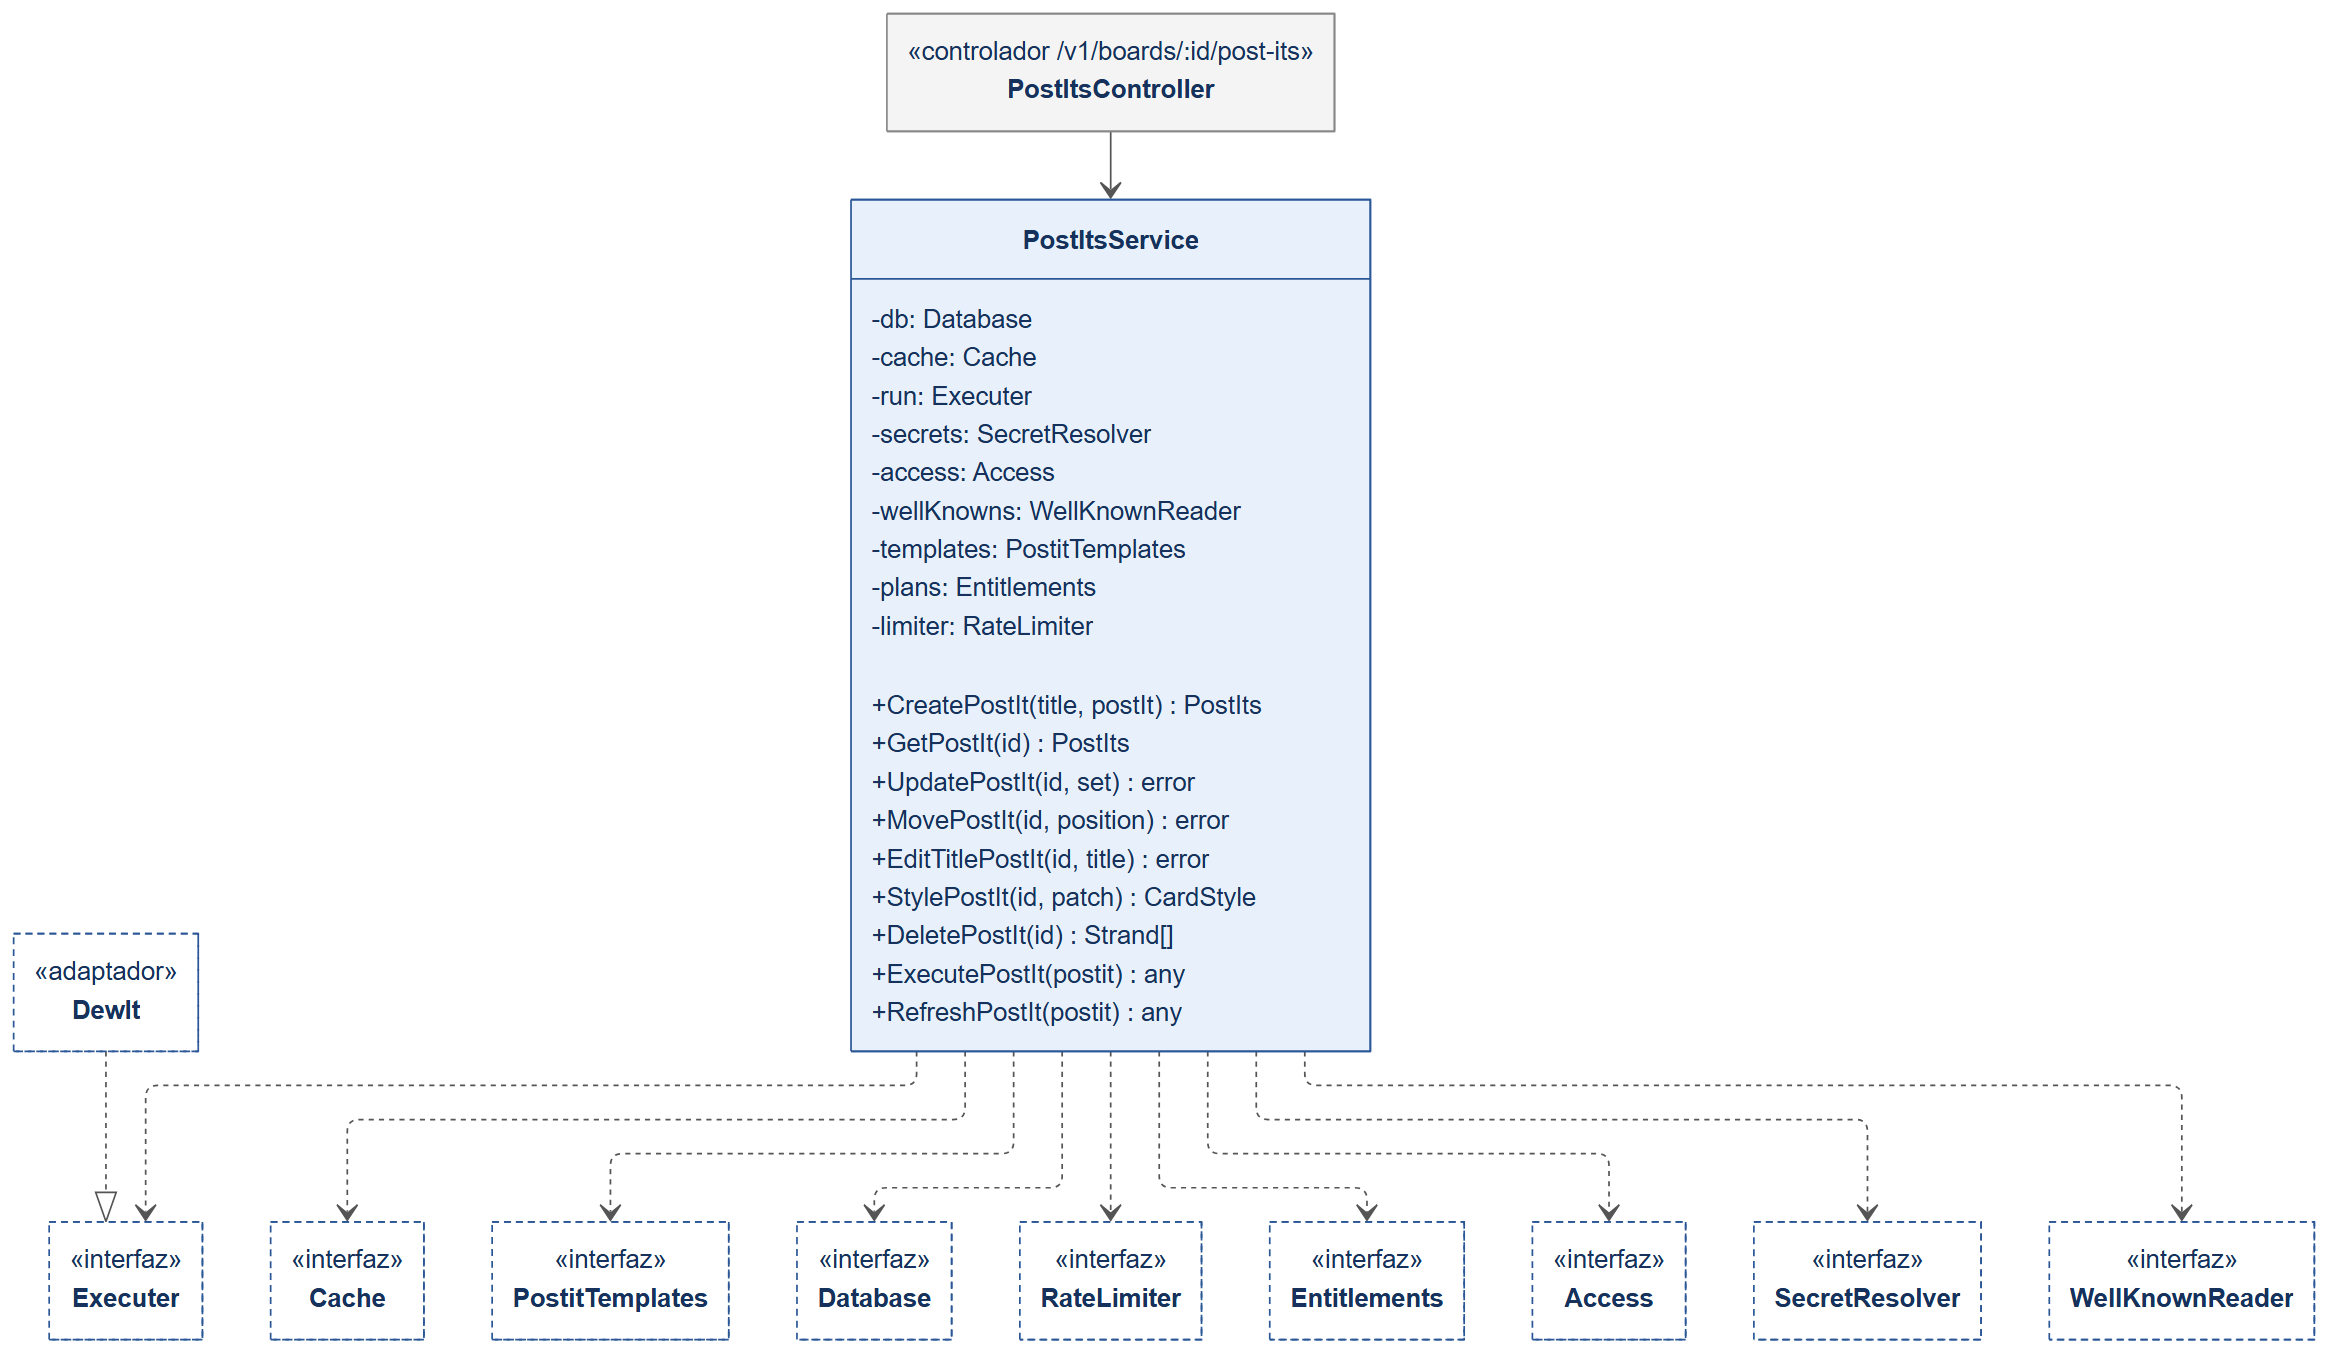
\includegraphics[width=0.95\textwidth]{figuras/fig22.png}
  \caption{Diagrama de clases del motor de tarjetas}
  \label{fig:clases_postits}
\end{figure}

Sus endpoints se resumen en la siguiente tabla.

\begin{tablaendpointsrol}{Endpoints de PostIts}{tab:endpoints_postits}
  POST & /post-its & Crear tarjeta (eventualmente desde un well-known). & editor \\
  GET & /post-its/\{id\} & Ejecutar la tarjeta y devolver el dato proyectado. & viewer \\
  GET & /post-its/\{id\}/settings & Obtener la configuración. & viewer \\
  PATCH & /post-its/\{id\}/settings & Editar params, bindings, query, response o rate, y para las tarjeta personalizada, también la URL y la petición. & editor \\
  PATCH & /post-its/\{id\}/position & Mover la tarjeta dentro del board. & editor \\
  PATCH & /post-its/\{id\}/title & Editar el título de la tarjeta. & editor \\
  PATCH & /post-its/\{id\}/style & Cambiar el estilo visual de la tarjeta (color, borde, alineación del texto y tamaño). & editor \\
  DELETE & /post-its/\{id\} & Eliminar la tarjeta y desreferenciar del board. & editor \\
\end{tablaendpointsrol}

\section{Integración con APIs}
El motor de integración, en el paquete \texttt{executer}, es responsable de resolver un PostIt a un valor concreto, cubriendo la capa de ejecución de los requisitos RF-07 y RF-08. Antes de invocarlo, el servicio de tarjetas prepara una copia del PostIt: cada placeholder \texttt{\$TOKEN} presente en \texttt{params}, \texttt{headers}, \texttt{queries} o en un valor del cuerpo JSON se mapea a una referencia de secreto, tomando el binding explícito de la tarjeta si existe. Esas referencias se resuelven como el principal \texttt{RunAs}, verificando nuevamente que pueda utilizarlas, y por último se inyectan los secretos de sistema que requiera el well-known. A continuación, cada llamada a \texttt{DewIt.Execute} recorre seis pasos.

En primer lugar, un short-circuit estático: si el campo \texttt{Resource} es nil, se devuelven los \texttt{Params} tal cual, lo que da soporte a las integraciones \texttt{static\_card} e \texttt{image} y a cualquier tarjeta sin fuente externa. Luego se elige el intérprete según el campo \texttt{response}: JSON con \texttt{gojq} o HTML con \texttt{goquery}. A continuación, la sustitución de variables, en la que \texttt{populate} reemplaza dentro de las queries y los headers aquellos valores cuyo contenido coincida con el nombre de un Param, identificados por el prefijo \texttt{\$}. En una petición \texttt{POST}, el cuarto paso aplica la misma sustitución a cada valor de texto del cuerpo JSON.

El quinto paso es la petición HTTP, creada con un \texttt{context.WithTimeout} de diez segundos, ensamblando querystring, headers y, si corresponde, el cuerpo como \texttt{application/json}, y exigiendo un status 200 OK; cualquier otro código se reporta como error de la tarjeta. Por último, el cuerpo de la respuesta, leído hasta un máximo de 2MB, se interpreta con el parser elegido: para JSON se compila cada expresión con \texttt{gojq.Parse} y se ejecuta con un timeout de doscientos cincuenta milisegundos, mientras que para HTML cada valor es un selector jquery evaluado con \texttt{goquery}, devolviendo al servicio un objeto con un valor por clave.

La siguiente tabla detalla las integraciones predefinidas que el sistema carga inicialmente en el catálogo.

\begingroup
\footnotesize
\setlength{\tabcolsep}{4.5pt}
\renewcommand{\arraystretch}{1.35}
\rowcolors{2}{gray!7}{white}
\begin{longtable}{
  >{\ttfamily\raggedright\arraybackslash}p{\dimexpr 0.21\textwidth - 2\tabcolsep\relax}
  >{\raggedright\arraybackslash}p{\dimexpr 0.20\textwidth - 2\tabcolsep\relax}
  >{\raggedright\arraybackslash}p{\dimexpr 0.33\textwidth - 2\tabcolsep\relax}
  >{\centering\arraybackslash}p{\dimexpr 0.10\textwidth - 2\tabcolsep\relax}
  >{\raggedright\arraybackslash}p{\dimexpr 0.16\textwidth - 2\tabcolsep\relax}
}
  \toprule
  \rowcolor{gray!18}
  \normalfont\bfseries Clave & \bfseries Fuente & \bfseries Query & \bfseries Rate & \bfseries Credencial \\
  \midrule
  \endfirsthead
  \toprule
  \rowcolor{gray!18}
  \normalfont\bfseries Clave & \bfseries Fuente & \bfseries Query & \bfseries Rate & \bfseries Credencial \\
  \midrule
  \endhead
  \midrule
  \rowcolor{white}
  \multicolumn{5}{r}{\textit{\scriptsize Continúa en la página siguiente...}} \\
  \endfoot
  \bottomrule
  \caption{Integraciones predefinidas actuales}
  \label{tab:integraciones_predefinidas}
  \endlastfoot
  static\_card & Interna & — & — & — \\
  image & Interna & — & — & — \\
  temperature & Open-Meteo & mín./máx. de temperatura horaria & 30 s & — \\
  air\_quality & Open-Meteo & Índice de calidad del aire, Material particulado 2.5 y fecha y hora de medida & 15 min & — \\
  events\_search & Ticketmaster & nombre, inicio de venta, imagen, fecha, lugar, ciudad y URL del primer evento & 120 s & del usuario \\
  dog\_facts & Dog API & atributos del primer fact & 5 s & — \\
  dolar\_oficial & dolarapi.com & compra/venta & 120 s & — \\
  exchange\_rate & currencyapi.com & código, valor y fecha & 60 min & del usuario \\
  riesgo\_pais & argentinadatos.com & valor y fecha & 60 min & — \\
  crypto\_price & CoinGecko & moneda, precio y variación en 24 h & 60 s & — \\
  nasa\_apod & NASA APOD & título, imagen, explicación y fecha & 60 min & de sistema \\
  gmail\_inbox & Gmail API & mensajes no leídos y totales & 60 s & OAuth2 (Google) \\
  google\_calendar & Google Calendar API & resumen e inicio del próximo evento & 5 min & OAuth2 (Google) \\
  github\_repo & GitHub API & nombre, estrellas, forks, issues y descripción del repositorio más popular & 5 min & — \\
\end{longtable}
\endgroup

El catálogo se almacena en la colección \texttt{well\_knowns} y lo administra el servicio \texttt{wellknowns}. Cada definición contiene la petición a realizar, la query de proyección, el rate por defecto, los parámetros que debe completar el usuario y las salidas que produce, con sus textos en español e inglés, además de los secretos de sistema que necesita. Los administradores de la plataforma pueden crear, modificar, eliminar y restaurar definiciones sin desplegar una nueva versión del backend.

El rate indicado es el valor por defecto de cada definición, y el tiempo que un resultado permanece en caché nunca es menor al mínimo del plan de quien paga el tablero (600, 150 o 60 segundos en los planes Free, Pro y Max, respectivamente).

La eliminación es lógica, de modo que las tarjetas creadas a partir de una definición borrada siguen funcionando. Durante las migraciones, el sistema carga las integraciones incorporadas que todavía no figuran en la colección, sin sobrescribir las que ya existen. Los placeholders de las definiciones se escriben en minúsculas (\texttt{\$credential}, \texttt{\$api\_key}), mientras que los nombres de los secretos del usuario van en mayúsculas (\texttt{\$MY\_KEY}), lo que evita colisiones entre ambos.

Los secretos del sistema, como la clave de la API de NASA, se resuelven al momento de la ejecución y nunca se almacenan en la tarjeta. Una integración personalizada, correspondiente al RF-08, reutiliza exactamente la misma estructura \texttt{PostIts} que un well-known, con el campo \texttt{WellKnown} vacío y todos los demás campos suministrados por el usuario, lo que la vuelve fácilmente extensible.

Las plantillas de tarjeta, en el paquete \texttt{postittemplates}, permiten guardar la configuración de una integración personalizada como un tipo de tarjeta reutilizable. Cada plantilla pertenece a un usuario, a un tablero o a una organización, y su clave comienza con el prefijo \texttt{custom\_} para no confundirse con las definiciones del catálogo. Quién puede verla, usarla o modificarla depende de ese ámbito, que se resuelve a través del puerto \texttt{Access}. Al crear una tarjeta a partir de una plantilla, esta se convierte a la misma forma que una definición del catálogo, por lo que el motor la ejecuta sin distinción. A diferencia del catálogo, una plantilla está en un único idioma, siempre realiza una petición \texttt{GET} y no puede utilizar secretos del sistema. La cantidad de plantillas de cada ámbito está limitada por el plan de quien lo paga, y eliminar una plantilla es definitivo: las tarjetas creadas a partir de ella siguen funcionando con su copia, pero ya no pueden editarse.

La Figura~\ref{fig:clases_wellknowns} muestra las clases de ambos servicios. \texttt{WellKnownService} administra el catálogo, mientras que \texttt{PostitTemplateService} implementa el puerto \texttt{PostitTemplates}, que el servicio de tarjetas consulta para obtener la definición de una plantilla utilizable en un tablero.

\begin{figure}[H]
  \centering
  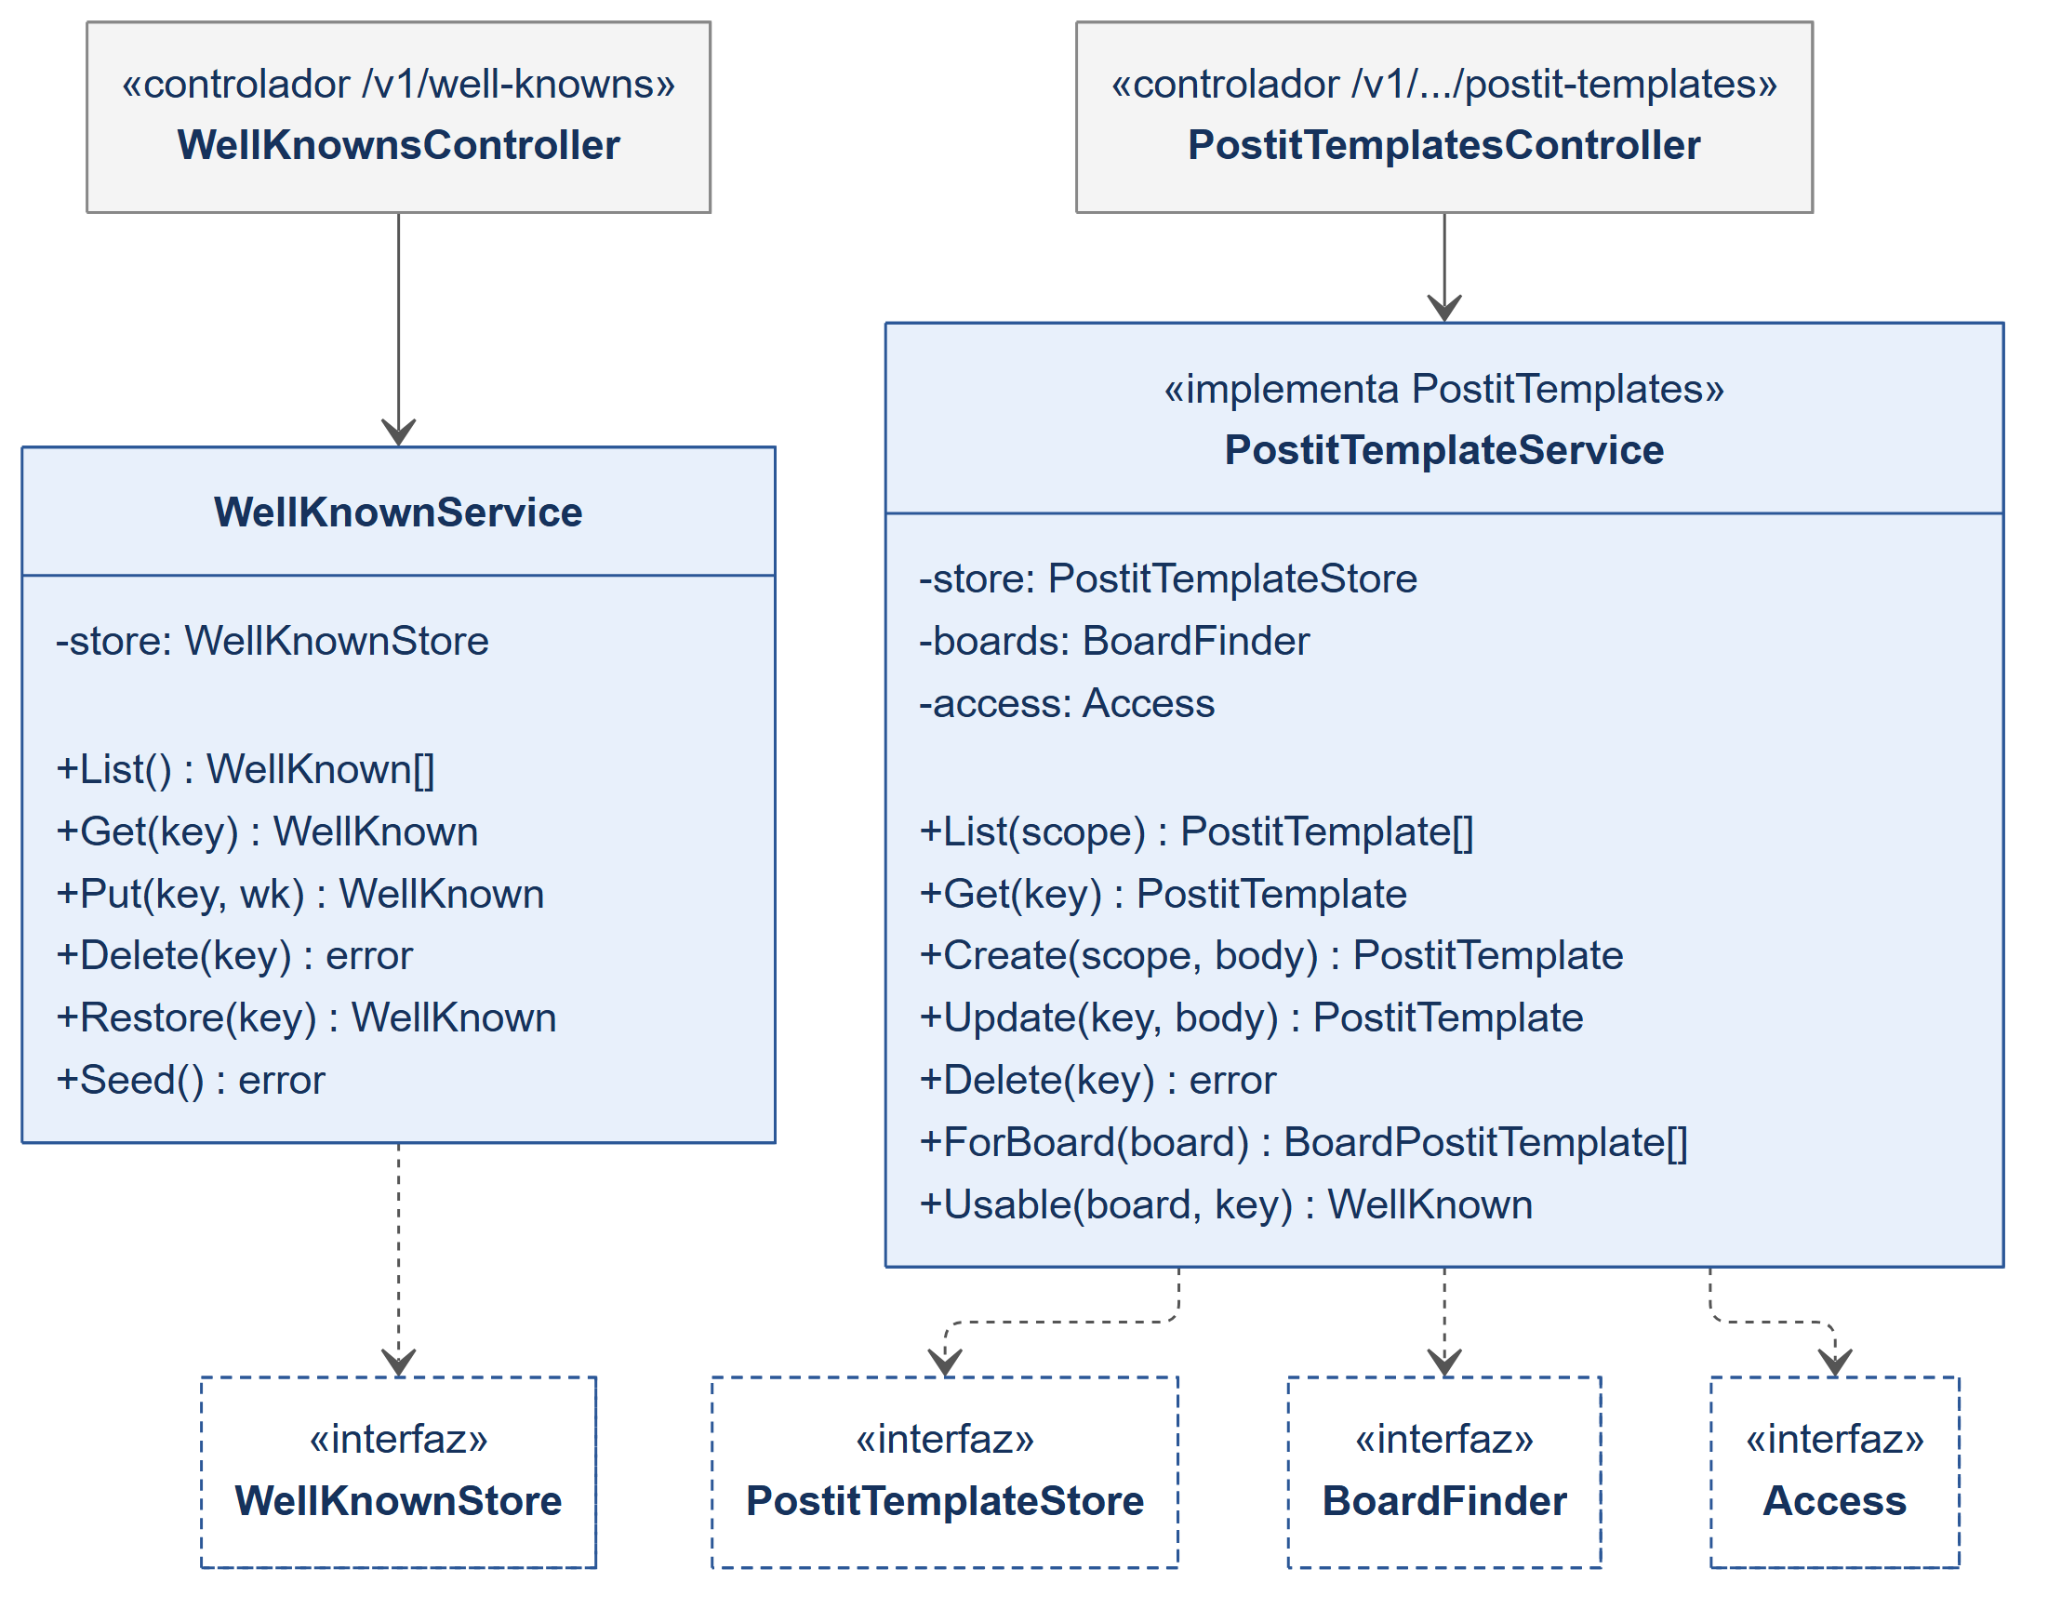
\includegraphics[width=0.92\textwidth]{figuras/fig23.png}
  \caption{Diagrama de clases del catálogo de integraciones y las plantillas de tarjeta}
  \label{fig:clases_wellknowns}
\end{figure}

Los endpoints del catálogo y de las plantillas se resumen en la Tabla~\ref{tab:endpoints_wellknowns}.

\begin{tablaendpointsrol}{Endpoints del catálogo y de las plantillas. \texttt{\{scope\}} corresponde a \texttt{/users/\{id\}}, \texttt{/boards/\{id\}} u \texttt{/orgs/\{id\}}.}{tab:endpoints_wellknowns}
  GET & /well-knowns & Listar el catálogo de integraciones. & usuario autenticado \\
  GET & /well-knowns/\{key\} & Obtener una definición del catálogo. & usuario autenticado \\
  PUT & /well-knowns/\{key\} & Crear o reemplazar una definición. & administrador \\
  DELETE & /well-knowns/\{key\} & Eliminar una definición (eliminación lógica). & administrador \\
  POST & /well-knowns/\{key\}/restore & Restaurar una definición eliminada. & administrador \\
  GET & \{scope\}/postit-templates & Listar las plantillas de un scope. & según el scope \\
  POST & \{scope\}/postit-templates & Crear una plantilla en el scope. & según el scope \\
  GET & /boards/\{id\}/postit-templates/usable & Listar las plantillas disponibles en un tablero. & viewer \\
  GET & /postit-templates/\{key\} & Obtener una plantilla. & según el scope \\
  PUT & /postit-templates/\{key\} & Modificar una plantilla. & según el scope \\
  DELETE & /postit-templates/\{key\} & Eliminar una plantilla. & según el scope \\
\end{tablaendpointsrol}

\section{Bóveda de secretos}
La bóveda, en el paquete \texttt{secrets}, es responsable de almacenar las credenciales que las tarjetas necesitan para consultar APIs privadas y de decidir quién puede gestionarlas, verlas y utilizarlas. Un secreto se identifica por su ámbito y su nombre, donde el ámbito puede ser un tablero (compartido con sus miembros), un miembro (lo que un usuario guarda para sí en un tablero), un usuario, un grupo o el sistema (reservado a los administradores de la plataforma).

Los valores se cifran con AES-GCM utilizando la clave de datos del ámbito, que a su vez se encuentra envuelta por un anillo de claves maestras versionado definido en \texttt{SECRETS\_MASTER\_KEYS}. Este esquema de cifrado por sobre permite rotar la clave maestra reenvolviendo únicamente las claves de datos, sin necesidad de recifrar cada secreto, y rotar la clave de un ámbito en particular cuando se sospecha de su compromiso.

La política de acceso, en \texttt{policy.go}, constituye la única costura de autorización de la bóveda y expone tres preguntas: \texttt{CanManage}, \texttt{CanView} y \texttt{CanUse}. Un principal puede utilizar un secreto en un tablero si es editor de ese tablero y, además, el ámbito lo admite o alguno de los grants del secreto lo alcanza. Los grants permiten compartir un secreto con un usuario, un grupo o un tablero, opcionalmente limitados a un tablero específico, sin revelar nunca su valor.

El diagrama de clases de la bóveda se presenta en la Figura~\ref{fig:clases_boveda}. La política queda aislada en la clase \texttt{policy}, que implementa \texttt{ScopePolicy}, y el servicio combina el almacenamiento de secretos y el anillo de claves con los puertos que requieren los flujos OAuth2: \texttt{TokenClient}, \texttt{Locker} y \texttt{HandshakeStore}. Además, consulta \texttt{GroupReader} y \texttt{Access} para resolver los grants, y \texttt{Entitlements} para limitar la cantidad de secretos según el plan de quien paga el ámbito.

\begin{figure}[H]
  \centering
  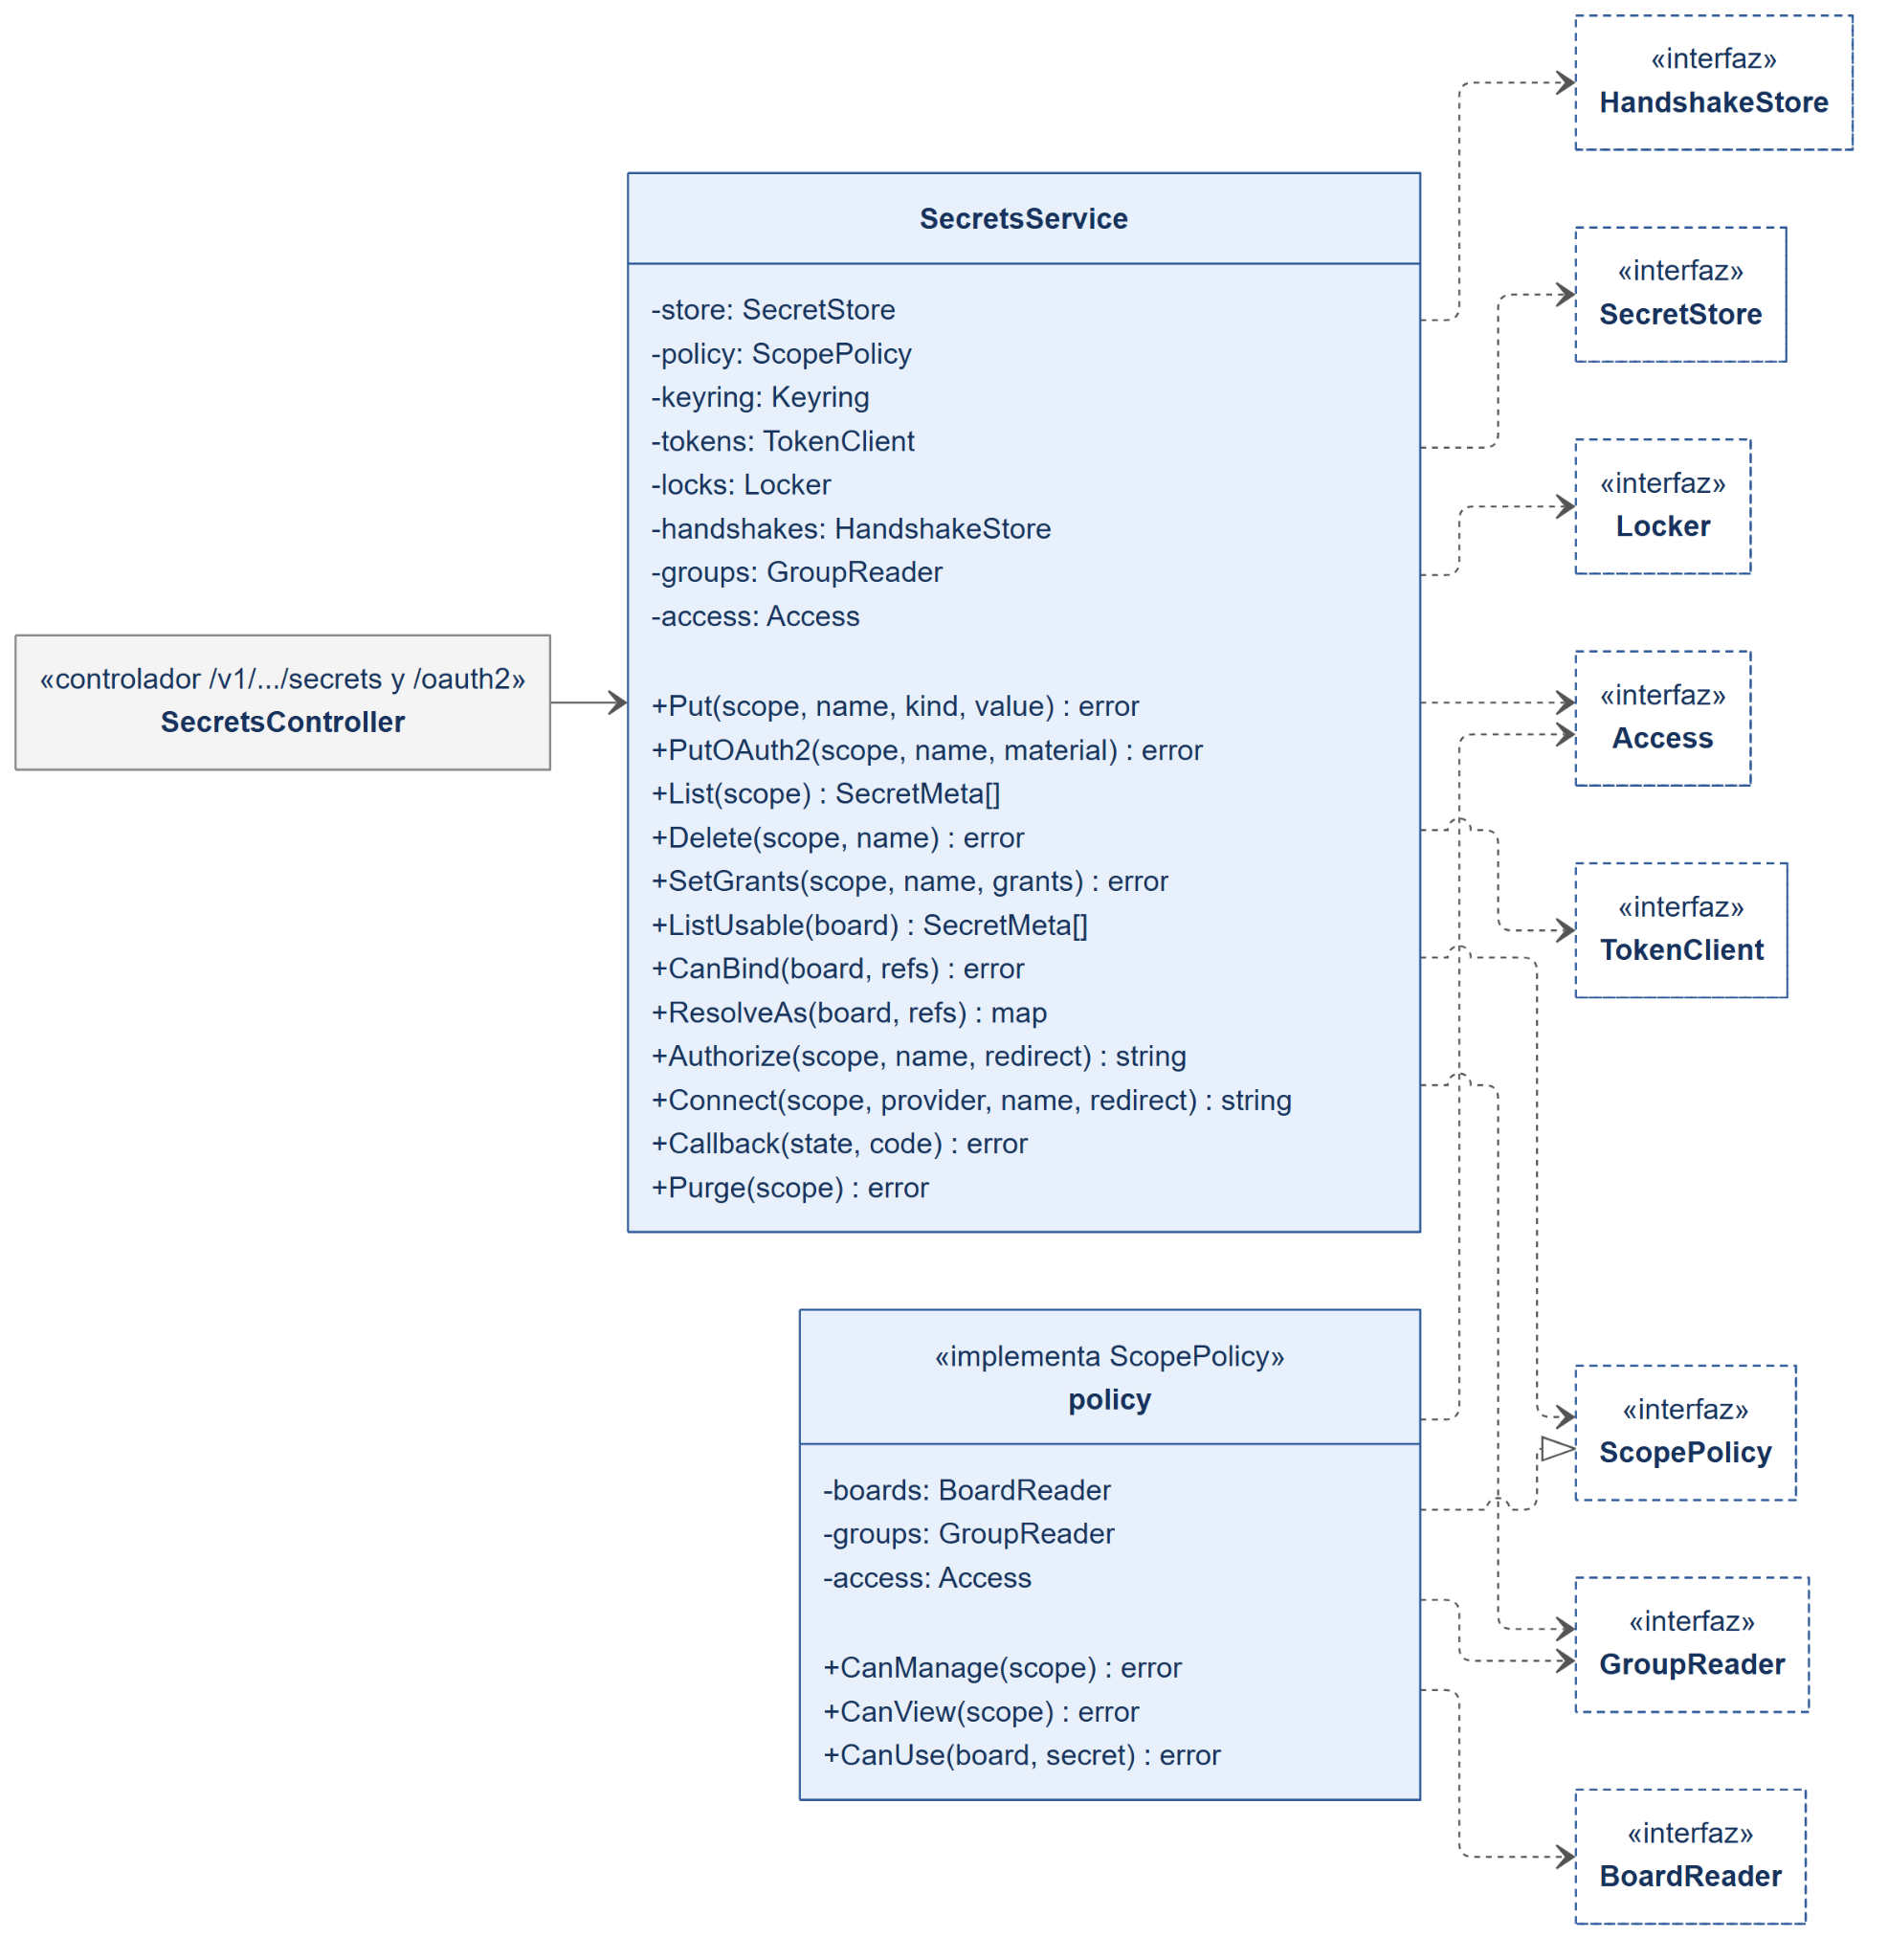
\includegraphics[width=0.92\textwidth]{figuras/fig24.png}
  \caption{Diagrama de clases de la bóveda de secretos}
  \label{fig:clases_boveda}
\end{figure}

\begin{tablaendpoints}{Endpoints de Secrets. \texttt{\{scope\}} corresponde a \texttt{/boards/\{id\}}, \texttt{/boards/\{id\}/members/\{user\}}, \texttt{/users/\{id\}} o \texttt{/groups/\{id\}}.}{tab:endpoints_secrets}
  GET & /\{scope\}/secrets & Listar la metadata de los secretos del ámbito. \\
  PUT & /\{scope\}/secrets & Crear o reemplazar un secreto (api\_key, bearer o basic). \\
  DELETE & /\{scope\}/secrets/\{name\} & Eliminar un secreto. \\
  PUT & /\{scope\}/secrets/\{name\}/grants & Definir con quién se comparte el secreto. \\
  PUT & /\{scope\}/oauth2 & Configurar una credencial OAuth2 con un cliente propio. \\
  GET & /\{scope\}/oauth2/authorize & Obtener la URL de consentimiento OAuth2. \\
  POST & /\{scope\}/oauth2/connect & Conectar una cuenta a través de un proveedor de la plataforma. \\
  GET & /boards/\{id\}/secrets/usable & Listar los secretos que el llamante puede vincular en el tablero. \\
  GET & /oauth2/providers & Listar los proveedores de la plataforma y si están configurados. \\
  GET & /oauth2/callback & Completar el consentimiento OAuth2 (solo quien lo inició). \\
  GET/PUT & /system/secrets & Listar o crear un secreto de sistema (solo administradores). \\
  DELETE & /system/secrets/\{name\} & Eliminar un secreto de sistema (solo administradores). \\
  PUT & /system/oauth2 & Configurar una credencial OAuth2 del ámbito sistema (solo administradores). \\
  PUT & /system/oauth2/clients & Configurar el cliente OAuth2 de un proveedor de la plataforma. \\
  GET & /system/keys & Listar el estado de las claves de datos. \\
\end{tablaendpoints}

Las credenciales OAuth2 pueden obtenerse con un cliente propio del usuario o a través de un proveedor administrado por la plataforma (Google, Discord), en cuyo caso el client id y el client secret se almacenan como secreto de sistema y se incorporan a la credencial únicamente en memoria. Los access tokens se renuevan automáticamente un minuto antes de su vencimiento, utilizando un lock distribuido en Redis para que dos ejecuciones concurrentes no consuman el mismo refresh token. Ningún handler devuelve jamás el valor de un secreto, un client secret ni un token. Cada secreto se descuenta del plan del usuario que paga su ámbito, registrado en \texttt{billed\_to}.

\section{Planes y facturación}
Este componente, materializado en los paquetes \texttt{entitlements} y \texttt{billing} y en el adaptador \texttt{mercadopago}, define qué permite cada plan y cobra las suscripciones de los planes pagos.

Cada usuario tiene un plan (\texttt{free}, \texttt{pro} o \texttt{max}) y una fecha de vencimiento opcional. Los límites de cada plan forman una única tabla en el código, que el frontend recibe para mostrarlos: cantidad de organizaciones, tableros por espacio, asientos, tarjetas por tablero, plantillas por ámbito, secretos y grupos, el tiempo mínimo de un resultado en caché, y si el plan permite forzar actualizaciones y usar tokens personales.

El servicio \texttt{entitlements} resuelve, para cada recurso, quién lo paga: un tablero personal lo paga su dueño, uno de organización el pagador de la organización, y un secreto el usuario indicado en \texttt{billed\_to}. Los demás servicios consultan este puerto antes de crear algo y, si el plan del pagador no lo admite, responden 402 con el nombre del límite alcanzado, su máximo y el plan vigente. Solo se rechazan las creaciones nuevas, de modo que una cuenta que baja de plan conserva lo que ya tiene.

El cobro se realiza mediante suscripciones mensuales de Mercado Pago, con un precio en pesos calculado a partir del precio en dólares de cada plan. Al suscribirse, el backend crea la suscripción y devuelve la URL del checkout del proveedor, que al finalizar redirige al frontend para sincronizarla. Cada cambio posterior llega por un webhook cuya firma HMAC se verifica, y el backend nunca confía en su contenido: ante cada notificación vuelve a leer la suscripción desde Mercado Pago. El plan queda vigente hasta cinco días después del próximo pago esperado, por lo que una suscripción cancelada o impaga vuelve sola al plan gratuito. Subir de plan se aplica de inmediato, mientras que bajarlo se aplica con la siguiente factura pagada.

Las clases que intervienen se muestran en la Figura~\ref{fig:clases_billing}. \texttt{EntitlementsService} implementa el puerto \texttt{Entitlements} que consultan los demás servicios, y para ello lee usuarios, organizaciones, tableros y grupos, y obtiene del puerto \texttt{Counter} los conteos de cada límite. \texttt{BillingService} depende del puerto \texttt{PaymentGateway}, implementado por el adaptador \texttt{Gateway} sobre el SDK de Mercado Pago, y de \texttt{SubscriptionStore} para guardar el estado conocido de cada suscripción.

\begin{figure}[H]
  \centering
  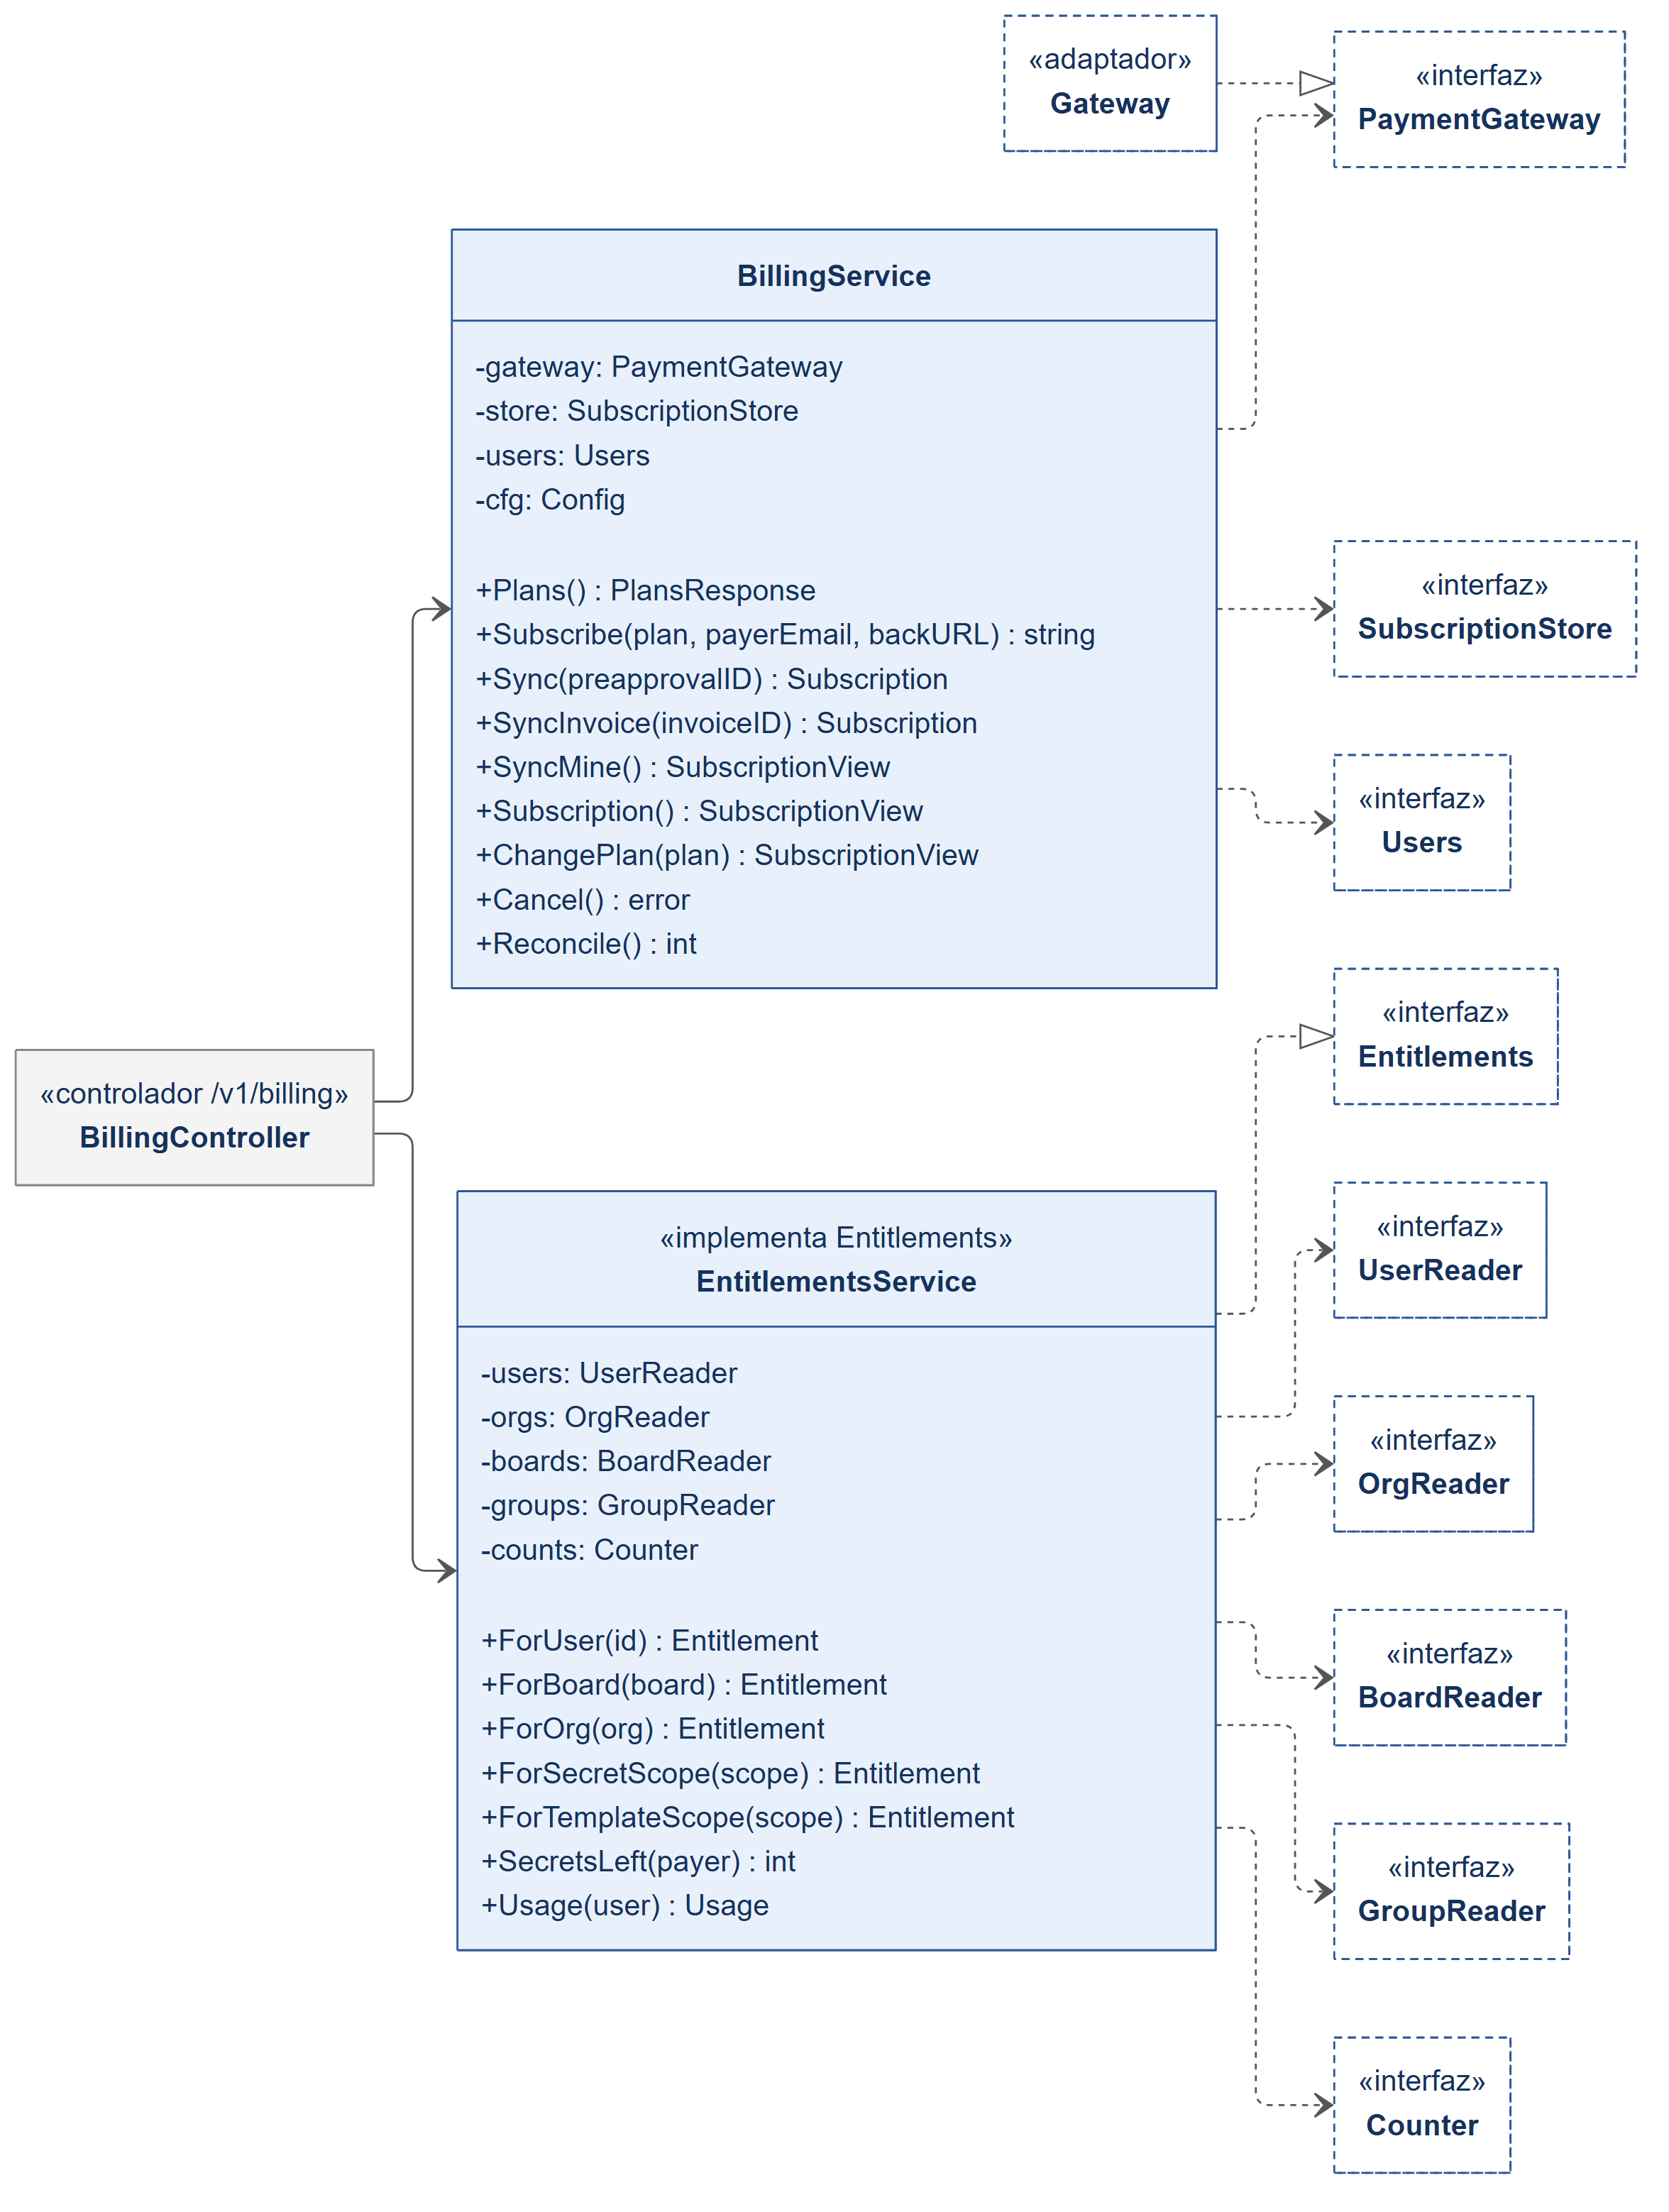
\includegraphics[width=0.85\textwidth]{figuras/fig41.png}
  \caption{Diagrama de clases de planes y facturación}
  \label{fig:clases_billing}
\end{figure}

Los endpoints de este componente se resumen en la Tabla~\ref{tab:endpoints_billing}.

\begin{tablaendpoints}{Endpoints de Billing}{tab:endpoints_billing}
  GET & /billing/plans & Listar los planes con sus límites y precios (público). \\
  POST & /billing/webhook & Recibir las notificaciones de Mercado Pago (público, con firma). \\
  GET & /billing/usage & Obtener el uso de la cuenta (organizaciones, grupos, secretos y plantillas). \\
  GET & /billing/subscription & Obtener el plan vigente y el estado de la suscripción. \\
  POST & /billing/subscribe & Iniciar una suscripción y obtener la URL del checkout. \\
  POST & /billing/sync & Sincronizar la suscripción tras volver del checkout. \\
  PUT & /billing/subscription & Cambiar de plan. \\
  DELETE & /billing/subscription & Cancelar la suscripción. \\
\end{tablaendpoints}

\section{Persistencia y caché}
Los adaptadores de persistencia y caché, en los paquetes \texttt{mongo} y \texttt{redis}, proveen las implementaciones concretas de los puertos de infraestructura de los que dependen los servicios.

El adaptador \texttt{mongo} implementa los puertos \texttt{Database}, \texttt{UserStore}, \texttt{GroupStore}, \texttt{OrgStore}, \texttt{SecretStore}, \texttt{KeyStore}, \texttt{AccessTokenStore}, \texttt{WellKnownStore}, \texttt{PostitTemplateStore} y \texttt{SubscriptionStore}, junto con las interfaces de solo lectura \texttt{UserReader}, \texttt{OrgReader}, \texttt{GroupReader} y \texttt{BoardReader}, encapsulando la lógica de persistencia descrita en los componentes anteriores, así como los conteos que necesita el servicio de planes para verificar cada límite. Al iniciar, \texttt{EnsureIndexes} crea de forma idempotente los índices de los que dependen las invariantes de unicidad, como el correo de cada usuario, el par \texttt{(scope, name)} de cada secreto o la existencia de una única clave de datos activa por ámbito.

Antes de crear los índices se ejecutan las migraciones, como el renombre de colecciones heredadas, y luego se carga el catálogo inicial de integraciones. En Vercel este paso no se ejecuta en cada arranque en frío, sino una única vez por despliegue de producción, mediante el comando \texttt{-migrate} durante la compilación.

El adaptador \texttt{redis}, por su parte, implementa el puerto \texttt{Caché} mediante las operaciones \texttt{FindPostItResult}, \texttt{AddPostItResult} y \texttt{DropPostItResult}, almacenando el último resultado de cada tarjeta bajo su identificador, con un tiempo de vida igual a su rate, y descartándolo cuando la tarjeta se edita o se elimina. Además, implementa las sesiones de refresco (claves \texttt{session:}, \texttt{spent:}, \texttt{family:} y \texttt{user-families:}), los límites de tasa (\texttt{rate:}, por ejemplo para inicios de sesión, invitaciones, creación de tokens y actualizaciones forzadas), los locks distribuidos (\texttt{lock:}) y los handshakes de los flujos OAuth2 (\texttt{oauth-handshake:}). La presencia de los usuarios en cada tablero (\texttt{board:\{id\}:online}) la escribe únicamente el servicio de tiempo real.

La relación entre estos adaptadores y los puertos que satisfacen se ilustra en la Figura~\ref{fig:adaptadores_persistencia}. Gracias a esta inversión de dependencias, cualquiera de estas tecnologías podría reemplazarse sin alterar la lógica de negocio. Cada círculo representa una interfaz provista por el adaptador, según la notación de UML.

\begin{figure}[H]
  \centering
  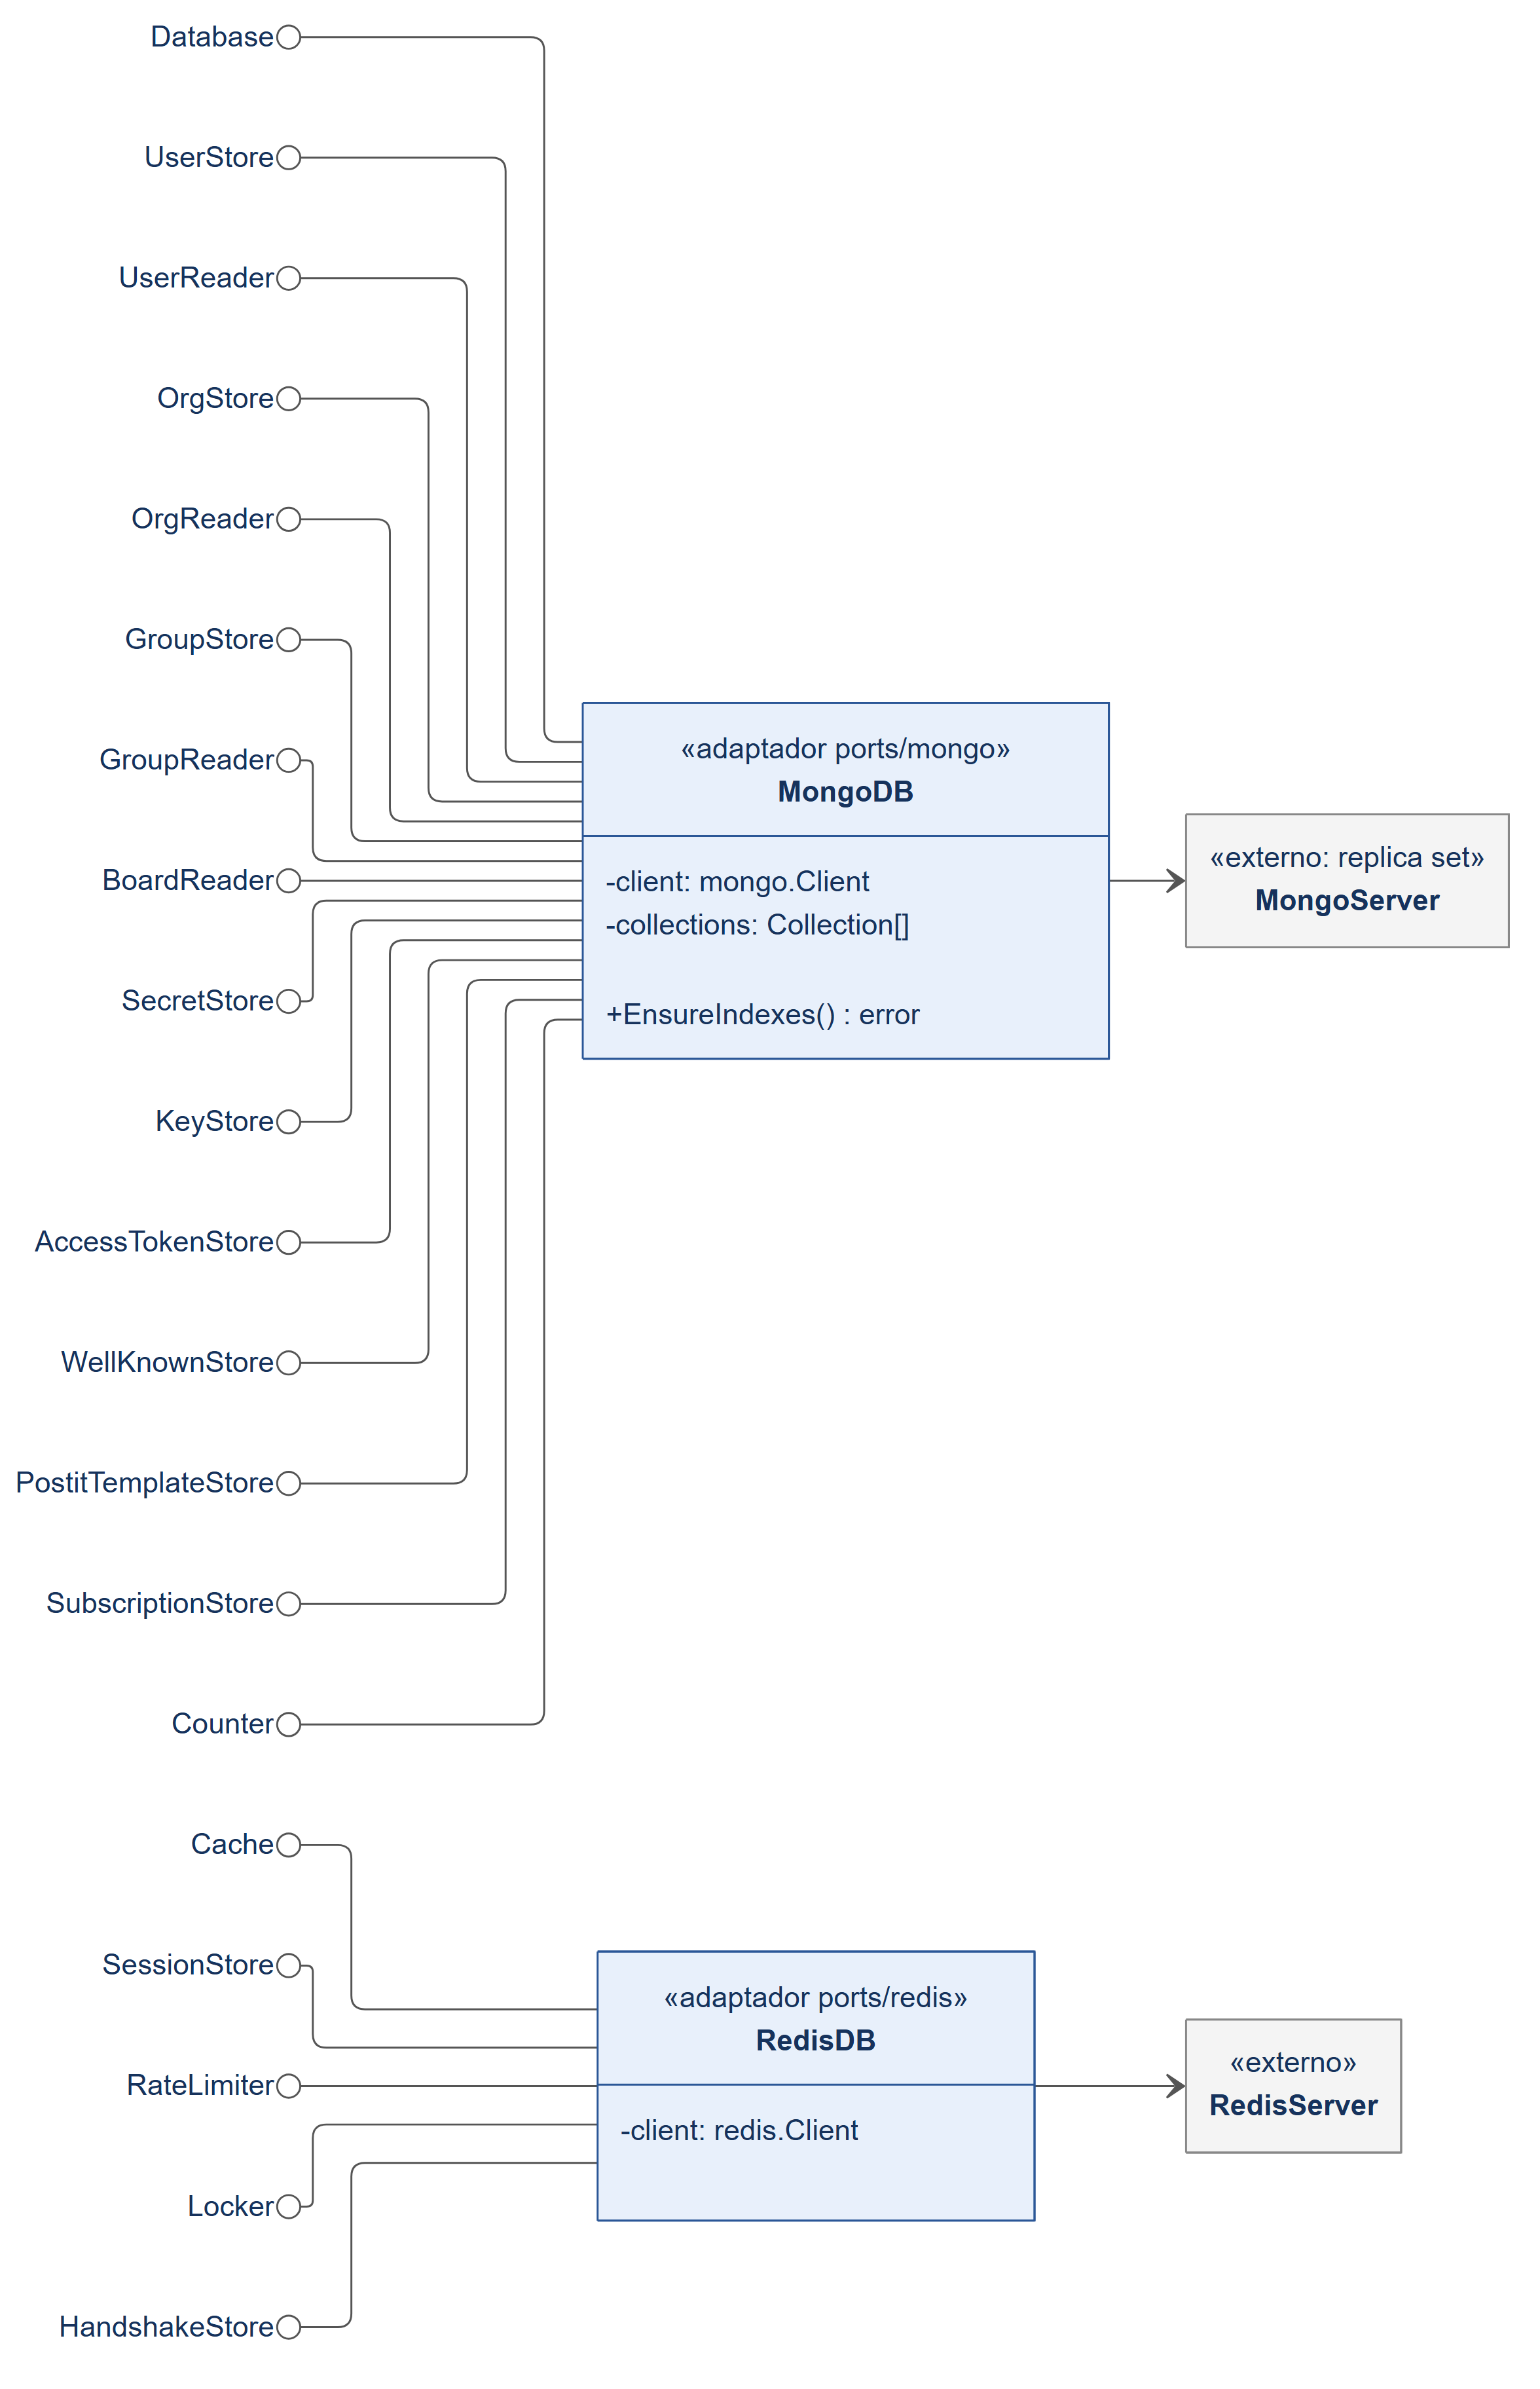
\includegraphics[width=0.78\textwidth]{figuras/fig25.png}
  \caption{Adaptadores de persistencia y puertos que implementan}
  \label{fig:adaptadores_persistencia}
\end{figure}

\section{Estrategia de actualización y caché}
A diferencia de los componentes anteriores, la actualización de las tarjetas no constituye un paquete independiente, sino una capacidad transversal que emerge de la colaboración entre el motor de tarjetas, el adaptador de caché y el frontend. Su objetivo es garantizar que las tarjetas reflejen el último dato disponible sin intervención del usuario, según lo establecido por el RF-09.

El mecanismo principal es un caché por tarjeta: al ejecutar una tarjeta, el servicio consulta primero Redis mediante \texttt{FindPostItResult} y, si existe un valor cacheado, lo devuelve sin tocar la fuente externa; en caso contrario, ejecuta el pipeline del executer y persiste el resultado con \texttt{AddPostItResult}, que aplica un \texttt{SET} con expiración igual al rate de la tarjeta o, si es menor, al tiempo mínimo que fija el plan, de modo que el tiempo de vida natural del dato coincide con su frecuencia de actualización sin que un rate muy bajo multiplique las consultas. Así, todos los usuarios que observan una misma tarjeta comparten un único resultado y la API externa se consulta como máximo una vez por período. Editar o eliminar la tarjeta descarta su resultado, y en el plan Max el usuario puede forzar una nueva ejecución. Este recorrido corresponde al diagrama de secuencia de la Figura~\ref{fig:seq_ejecucion}.

A esto se suma el header \texttt{Cache-Control: private, max-age=10} (o \texttt{no-store} en una actualización forzada) en la respuesta de ejecución, que permite que el navegador absorba parte de la carga, y el servicio de tiempo real, que notifica a cada cliente los cambios estructurales del tablero, como tarjetas agregadas, movidas o reconfiguradas, para que vuelva a cargarlo sin necesidad de polling.

\section{Notificaciones por correo}
El adaptador \texttt{mail} implementa el puerto \texttt{Mailer}, encargado de enviar los correos de verificación de cuenta y de recuperación de contraseña, así como el aviso que recibe el titular de una cuenta cuando alguien intenta registrarse con su correo, lo que evita revelar en la respuesta del registro si una dirección ya existe. Cada correo se renderiza a partir de plantillas embebidas en el binario, una por idioma, y se envía en el idioma preferido del destinatario. Al iniciar, el servicio verifica que cada plantilla exista en todos los idiomas soportados, rechazando el arranque en caso contrario.

El envío se delega en un \texttt{Sender} intercambiable: con la variable \texttt{RESEND\_API\_KEY} configurada se utiliza Resend, mientras que sin ella los correos se vuelcan al log, lo que permite desarrollar localmente sin un proveedor externo.

La Figura~\ref{fig:clases_mail} muestra las clases del adaptador. \texttt{Mailer} implementa el puerto del mismo nombre y combina las plantillas, que generan el asunto y los cuerpos en texto y HTML, con un \texttt{Sender}, cuya implementación se elige al iniciar según la configuración.

\begin{figure}[H]
  \centering
  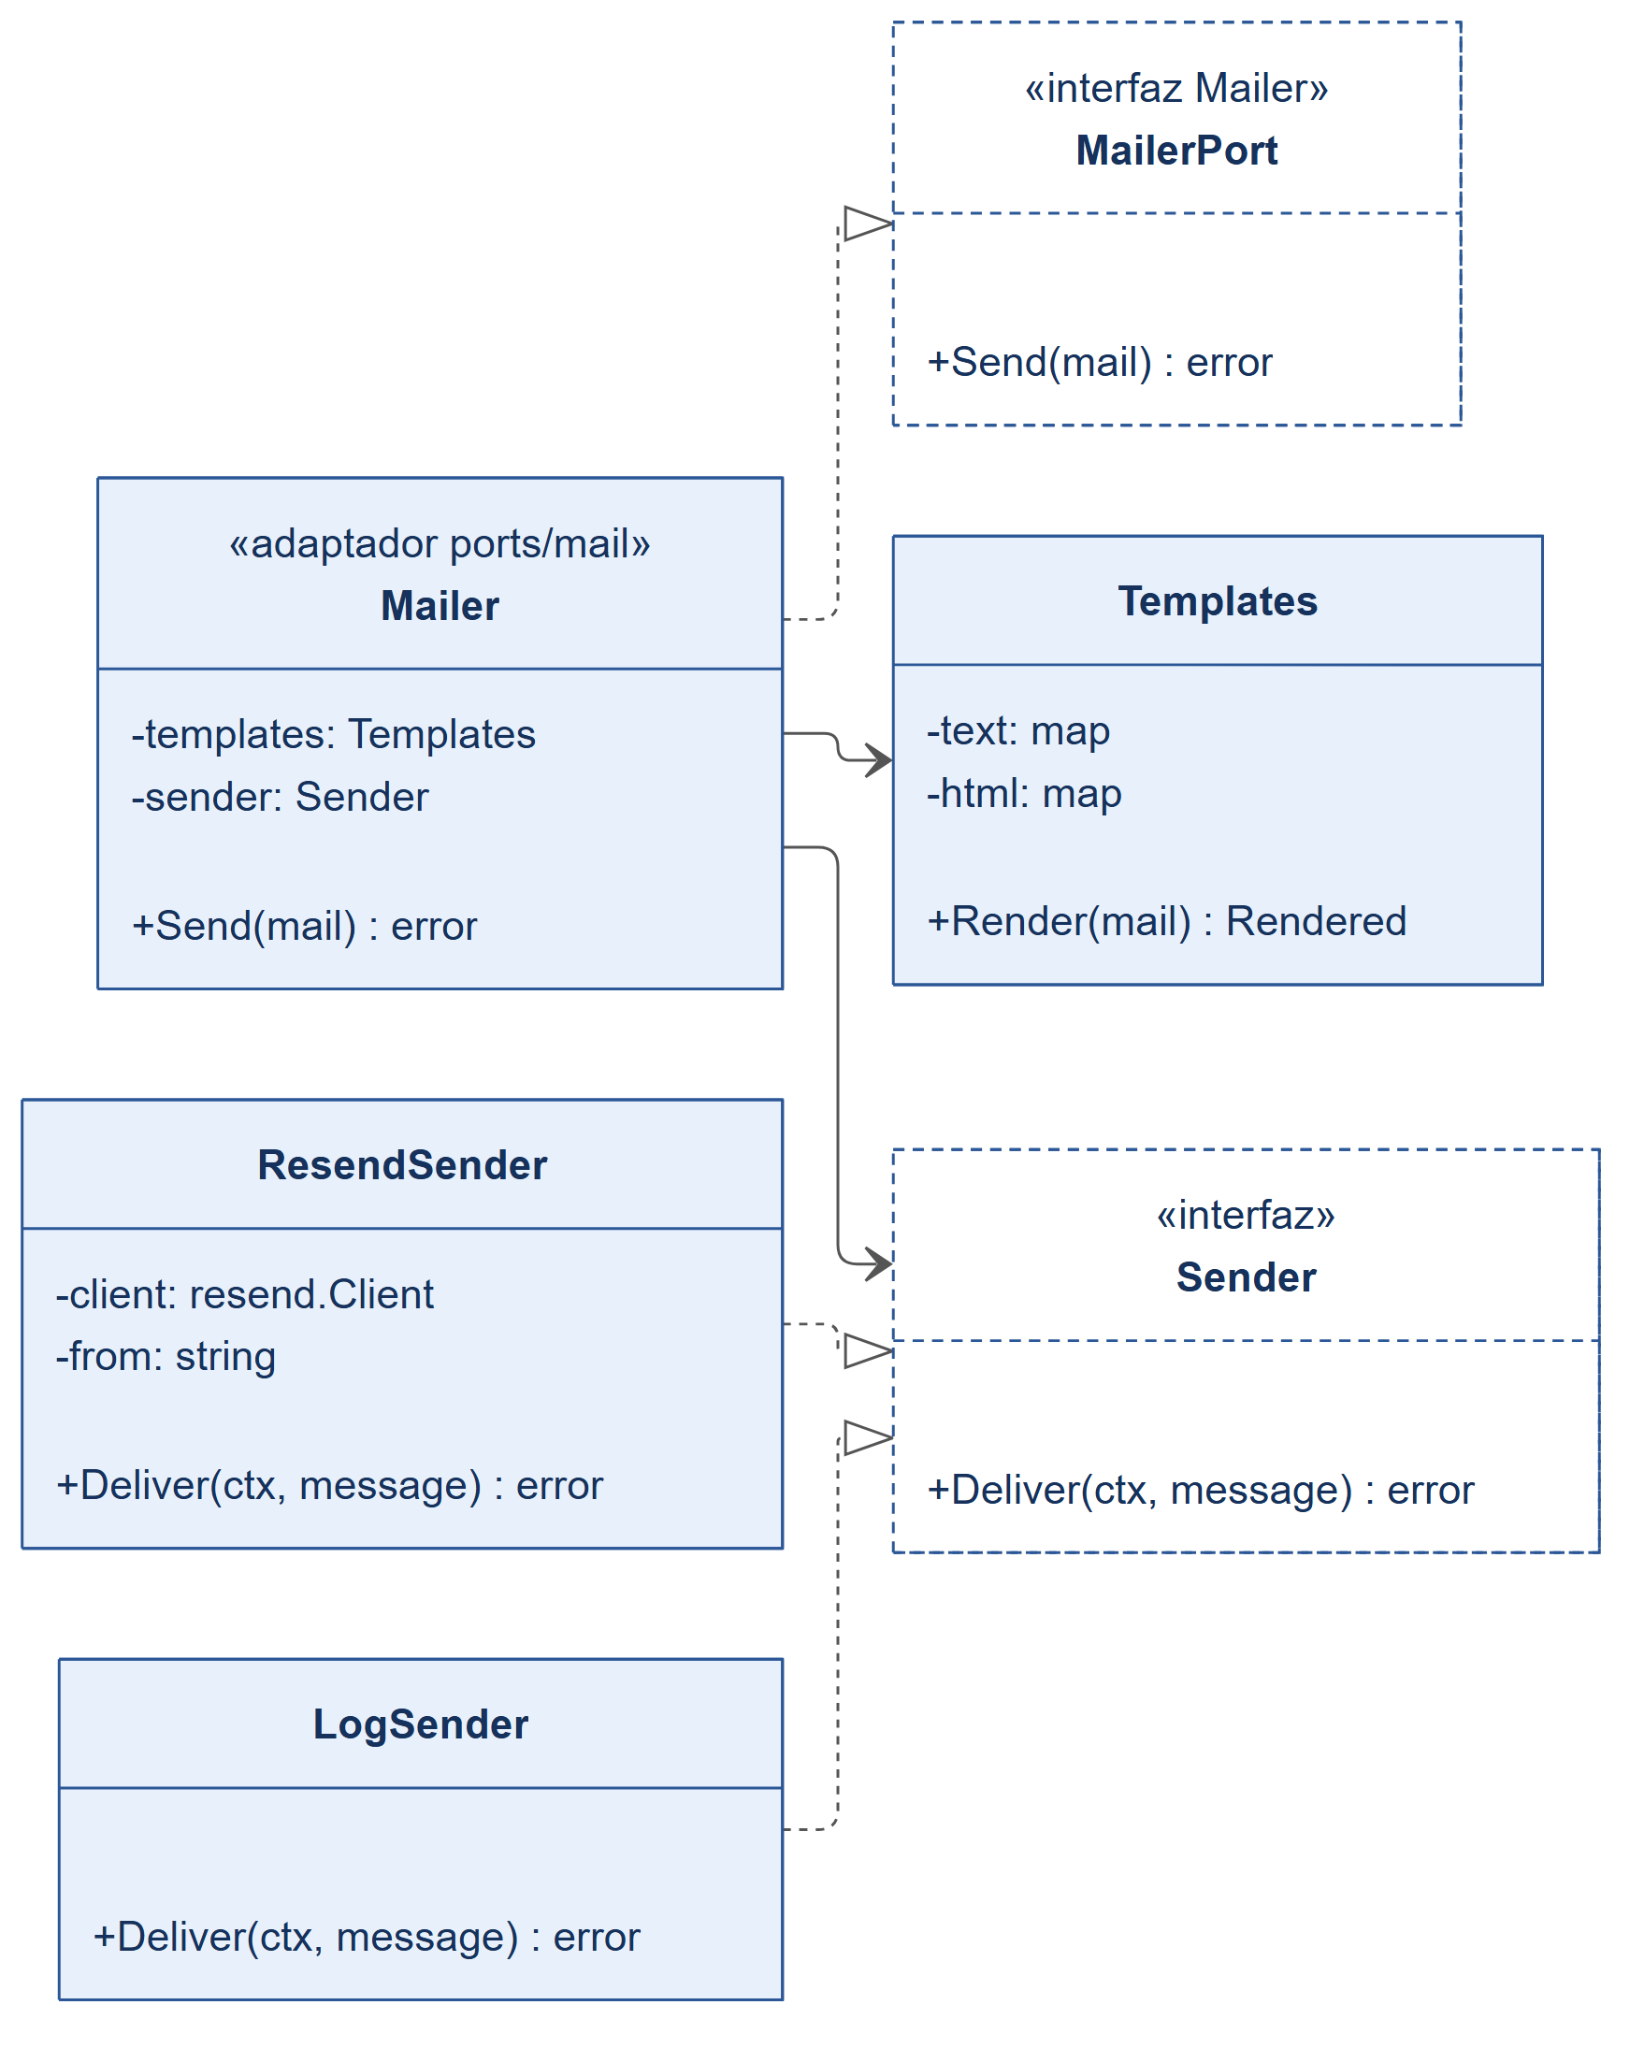
\includegraphics[width=0.72\textwidth]{figuras/fig26.png}
  \caption{Diagrama de clases del adaptador de correo}
  \label{fig:clases_mail}
\end{figure}

\section{Tiempo real}
El servicio de tiempo real, en la carpeta \texttt{realtime}, es un proceso Node independiente del backend encargado de propagar los cambios de un tablero a todos los usuarios conectados. Escucha la colección \texttt{boards} mediante un change stream de MongoDB y, ante cada actualización, emite un evento \texttt{update} a la sala de \texttt{socket.io} correspondiente al tablero.

Al conectarse, el cliente envía su token de acceso y el servicio consulta al backend \texttt{GET /boards/\{id\}} con ese mismo token: si no obtiene un 200 con un rol, rechaza la conexión. De esta forma, el servicio nunca verifica un JWT por sí mismo y el backend sigue siendo la única autoridad de autorización. Un minuto antes de que el token expire, el servidor solicita uno nuevo y vuelve a verificar el rol, de modo que un miembro removido pierde las actualizaciones a más tardar en la siguiente renovación. Si el cliente no presenta un token nuevo dentro de los treinta segundos posteriores al vencimiento, se lo desconecta.

La presencia de los usuarios en cada tablero se mantiene en el hash \texttt{board:\{id\}:online} de Redis, mientras que los cursores se comparten de manera peer-to-peer mediante WebRTC (PeerJS), sin pasar por el servidor. La entrada de presencia expira veinte minutos después de la última conexión o renovación.

La organización interna del servicio se representa en la Figura~\ref{fig:modulos_realtime}. El módulo \texttt{mongo} recibe los cambios del change stream y se los entrega a \texttt{socket}, que administra las salas. Este último consulta los roles a través de \texttt{auth}, que a su vez interroga al backend, y registra la presencia mediante el módulo \texttt{redis}.

\begin{figure}[H]
  \centering
  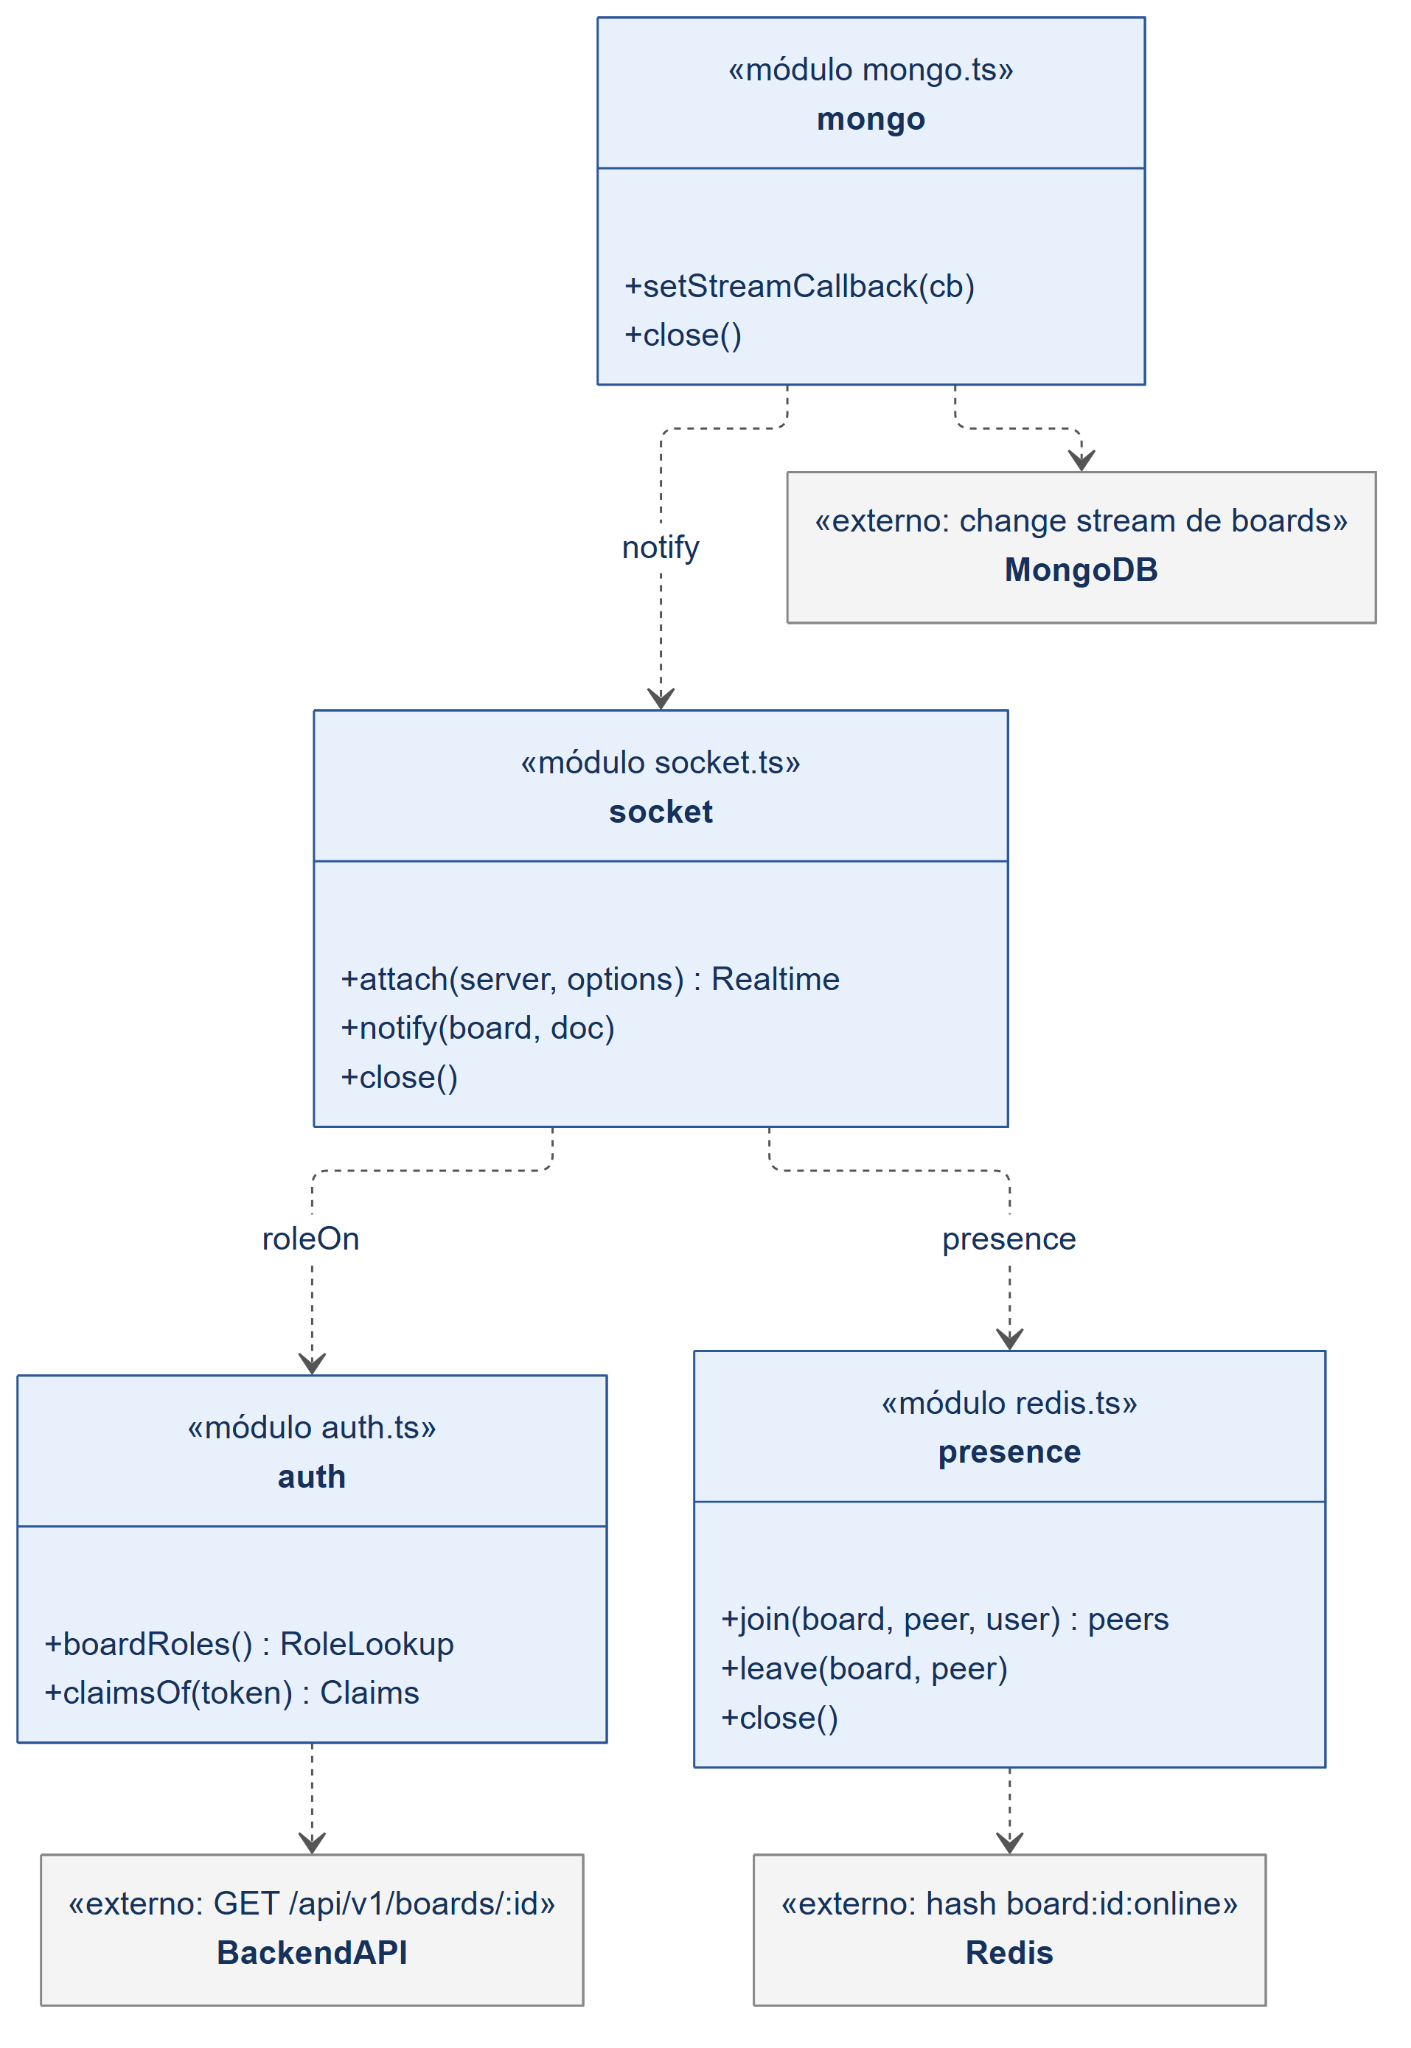
\includegraphics[width=0.75\textwidth]{figuras/fig27.png}
  \caption{Módulos del servicio de tiempo real}
  \label{fig:modulos_realtime}
\end{figure}
% !TEX root = ../main.tex
\chapter{Especificación de Casos de Prueba (MVP) y Resultados}

\section{Especificación de Casos de Prueba (MVP)}
Para validar el incremento actual se definieron tres familias de pruebas: pruebas de funcionalidad, que verifican cada requisito funcional implementado de forma aislada sobre la API; pruebas de interfaz con usuarios reales, orientadas a garantizar la usabilidad del tablero; y pruebas de seguridad, centradas en los requisitos no funcionales críticos, en particular el almacenamiento seguro de credenciales del RNF-02. A continuación se presentan los casos correspondientes a las funcionalidades ya implementadas.

\subsection{Casos de prueba de funcionalidad}
Estos casos verifican el comportamiento esperado de cada endpoint implementado, mapeando cada prueba al requisito funcional que cubre.

\begin{longtable}{>{\bfseries}l >{\bfseries}l p{0.36\textwidth} p{0.38\textwidth}}
  \toprule
  ID & RF & Qué se prueba & Resultado esperado \\
  \midrule
  \endfirsthead
  \toprule
  ID & RF & Qué se prueba & Resultado esperado \\
  \midrule
  \endhead
  \bottomrule
  \caption{Casos de prueba de funcionalidad}
  \label{tab:cp_funcionalidad}
  \endfoot
  CP-01 & RF-04 & Creación de un tablero vacío. & El tablero se crea y aparece en el listado del usuario. \\
  CP-02 & RF-05 & Agregado de una tarjeta al tablero. & La tarjeta se crea y queda asociada al tablero en su posición inicial. \\
  CP-03 & RF-06 & Conexión de dos tarjetas mediante un hilo. & La strand se crea y queda persistida en el tablero. \\
  CP-04 & RF-06 & Conexión con una tarjeta inexistente. & La operación es rechazada, evitando hilos colgantes. \\
  CP-05 & RF-06 & Eliminación de una tarjeta conectada. & Se elimina la tarjeta y sus strands asociadas, sin afectar las demás. \\
  CP-06 & RF-07 & Ejecución de una integración predefinida (\texttt{dolar\_oficial}). & La tarjeta devuelve los datos esperados de la fuente externa. \\
  CP-07 & RF-07 & Integración predefinida sin un parámetro requerido. & Se reporta un error explícito por la variable faltante. \\
  CP-08 & RF-08 & Conexión a una API externa personalizada. & La tarjeta muestra el dato proyectado a partir de la respuesta. \\
  CP-09 & RF-08 & Conexión a una URL inválida. & La tarjeta reporta el error sin romper el resto del tablero. \\
  CP-10 & RF-09 & Lectura repetida dentro del intervalo de rate. & La segunda lectura se sirve del caché; al expirar el rate, se refresca. \\
\end{longtable}

\subsection{Casos de prueba con usuarios para validar la interfaz}
Estas pruebas se realizan en sesiones moderadas con usuarios de perfil técnico y no técnico, observando cómo completan tareas concretas sobre el tablero sin asistencia previa, con el fin de detectar problemas de usabilidad.

\begin{table}[H]
  \centering
  \renewcommand{\arraystretch}{1.2}
  \begin{tabularx}{\textwidth}{>{\bfseries}l X X}
    \toprule
    ID & Tarea del usuario & Métrica de éxito \\
    \midrule
    UX-01 & Crear un tablero y agregar una primera tarjeta. & La completa sin asistencia ni necesidad de documentación. \\
    UX-02 & Conectar dos tarjetas con un hilo. & Descubre el gesto del hilo por sí mismo. \\
    UX-03 & Cambiar la configuración de una tarjeta predefinida. & Lo logra en pocos segundos y sin errores irrecuperables. \\
    UX-04 & Conectar una tarjeta a una API personalizada (perfil técnico). & Logra mostrar un dato en un tiempo razonable. \\
    UX-05 & Recuperarse de una configuración con una URL inválida. & Identifica el error y lo corrige sin perder la tarjeta. \\
    \bottomrule
  \end{tabularx}
  \caption{Casos de prueba de interfaz}
  \label{tab:cp_ux}
\end{table}

\subsection{Casos de prueba de seguridad}
Estas pruebas validan el almacenamiento seguro de credenciales exigido por el RNF-02, así como los controles de acceso propios de un sistema multiusuario.

\begin{table}[H]
  \centering
  \renewcommand{\arraystretch}{1.2}
  \begin{tabularx}{\textwidth}{>{\bfseries}l X X}
    \toprule
    ID & Qué se prueba & Resultado esperado \\
    \midrule
    SEC-01 & Almacenamiento de las credenciales de una API personalizada. & Las credenciales no se guardan en texto plano en la base de datos. \\
    SEC-02 & Exposición de credenciales al cliente. & La configuración devuelta al frontend omite los valores sensibles. \\
    SEC-03 & Acceso de un usuario a un tablero ajeno. & El acceso es rechazado; solo el dueño y los colaboradores pueden verlo. \\
    SEC-04 & Ejecución de una expresión de proyección costosa. & El timeout aborta la query sin afectar al resto del proceso. \\
    \bottomrule
  \end{tabularx}
  \caption{Casos de prueba de seguridad}
  \label{tab:cp_seguridad}
\end{table}

\section{Resultados de Testing}
Se desarrollaron los tests unitarios, de integración y de punta a punta, con el objeto de corroborar la correcta implementación del sistema en base a las pruebas definidas. Se configuró un sistema de CI/CD para asegurar la consistencia del código fuente a medida que avanza el equipo. En la Tabla~\ref{tab:resultados_testing} se resumen los resultados de la última ejecución.

En el backend, la cobertura se calcula sobre los paquetes propios, excluyendo los adaptadores de MongoDB y Redis, que se validan con 52 pruebas de integración ejecutadas contra instancias reales de ambas bases y un servidor OAuth2 simulado. Las suites del backend y del servicio de tiempo real se ejecutan automáticamente en GitHub Actions ante cada cambio, mientras que las del frontend se ejecutan de forma local.

\begin{table}[H]
  \centering
  \renewcommand{\arraystretch}{1.2}
  \begin{tabularx}{\textwidth}{>{\bfseries}l X r l}
    \toprule
    Servicio & Tipo de pruebas & Tests & Cobertura \\
    \midrule
    Backend (Go) & Unitarias y de controladores & 474 & 81,7 \% de sentencias \\
    Backend (Go) & Integración con MongoDB, Redis y OAuth2 simulado & 52 & No aplica \\
    Tiempo real (Node.js) & Unitarias & 19 & 97,5 \% de líneas \\
    Frontend (SvelteKit) & Unitarias de módulos y lógica & 91 & 39,3 \% de sentencias \\
    Servidor MCP (xmcp) & Sin pruebas automatizadas & 0 & No aplica \\
    \bottomrule
  \end{tabularx}
  \caption{Resultados de las pruebas automatizadas por servicio}
  \label{tab:resultados_testing}
\end{table}

Las pruebas de usabilidad se desarrollaron con un grupo selecto de personas, siguiendo el modelo de usuarios representativos. Se construyó un diseño preliminar de la web en Figma, y a partir de la misma se iteró con los usuarios hasta conseguir un nivel de éxito aceptable según el equipo.

\section{MVP en producción y vistas de la interfaz}
El desarrollo se encuentra actualmente en producción, disponible desde la url del sitio web. Se compró un dominio para la entrega final, con el objeto de hacer más fácil de recordar el nombre del producto y la url.

\begin{itemize}
  \item \textbf{Link a la web:} \url{https://corcheria.company/}
  \item \textbf{Link al repo de bitbucket:} \url{https://bitbucket.org/itba/pf-2026a-tablero-informacion-universal/src/main/}
  \item \textbf{Link al repo de Github:} \url{https://github.com/Tobias-Noceda/tablero-informacion-universal}
\end{itemize}

El acceso a la aplicación comienza con el inicio de sesión, que admite correo y contraseña o una cuenta de Google, y con el registro de nuevos usuarios, quienes deben verificar su correo antes de ingresar (RF-01 y RF-02). Las Figuras~\ref{fig:ui_login} y \ref{fig:ui_registro} muestran ambas pantallas.

\begin{figure}[H]
  \centering
  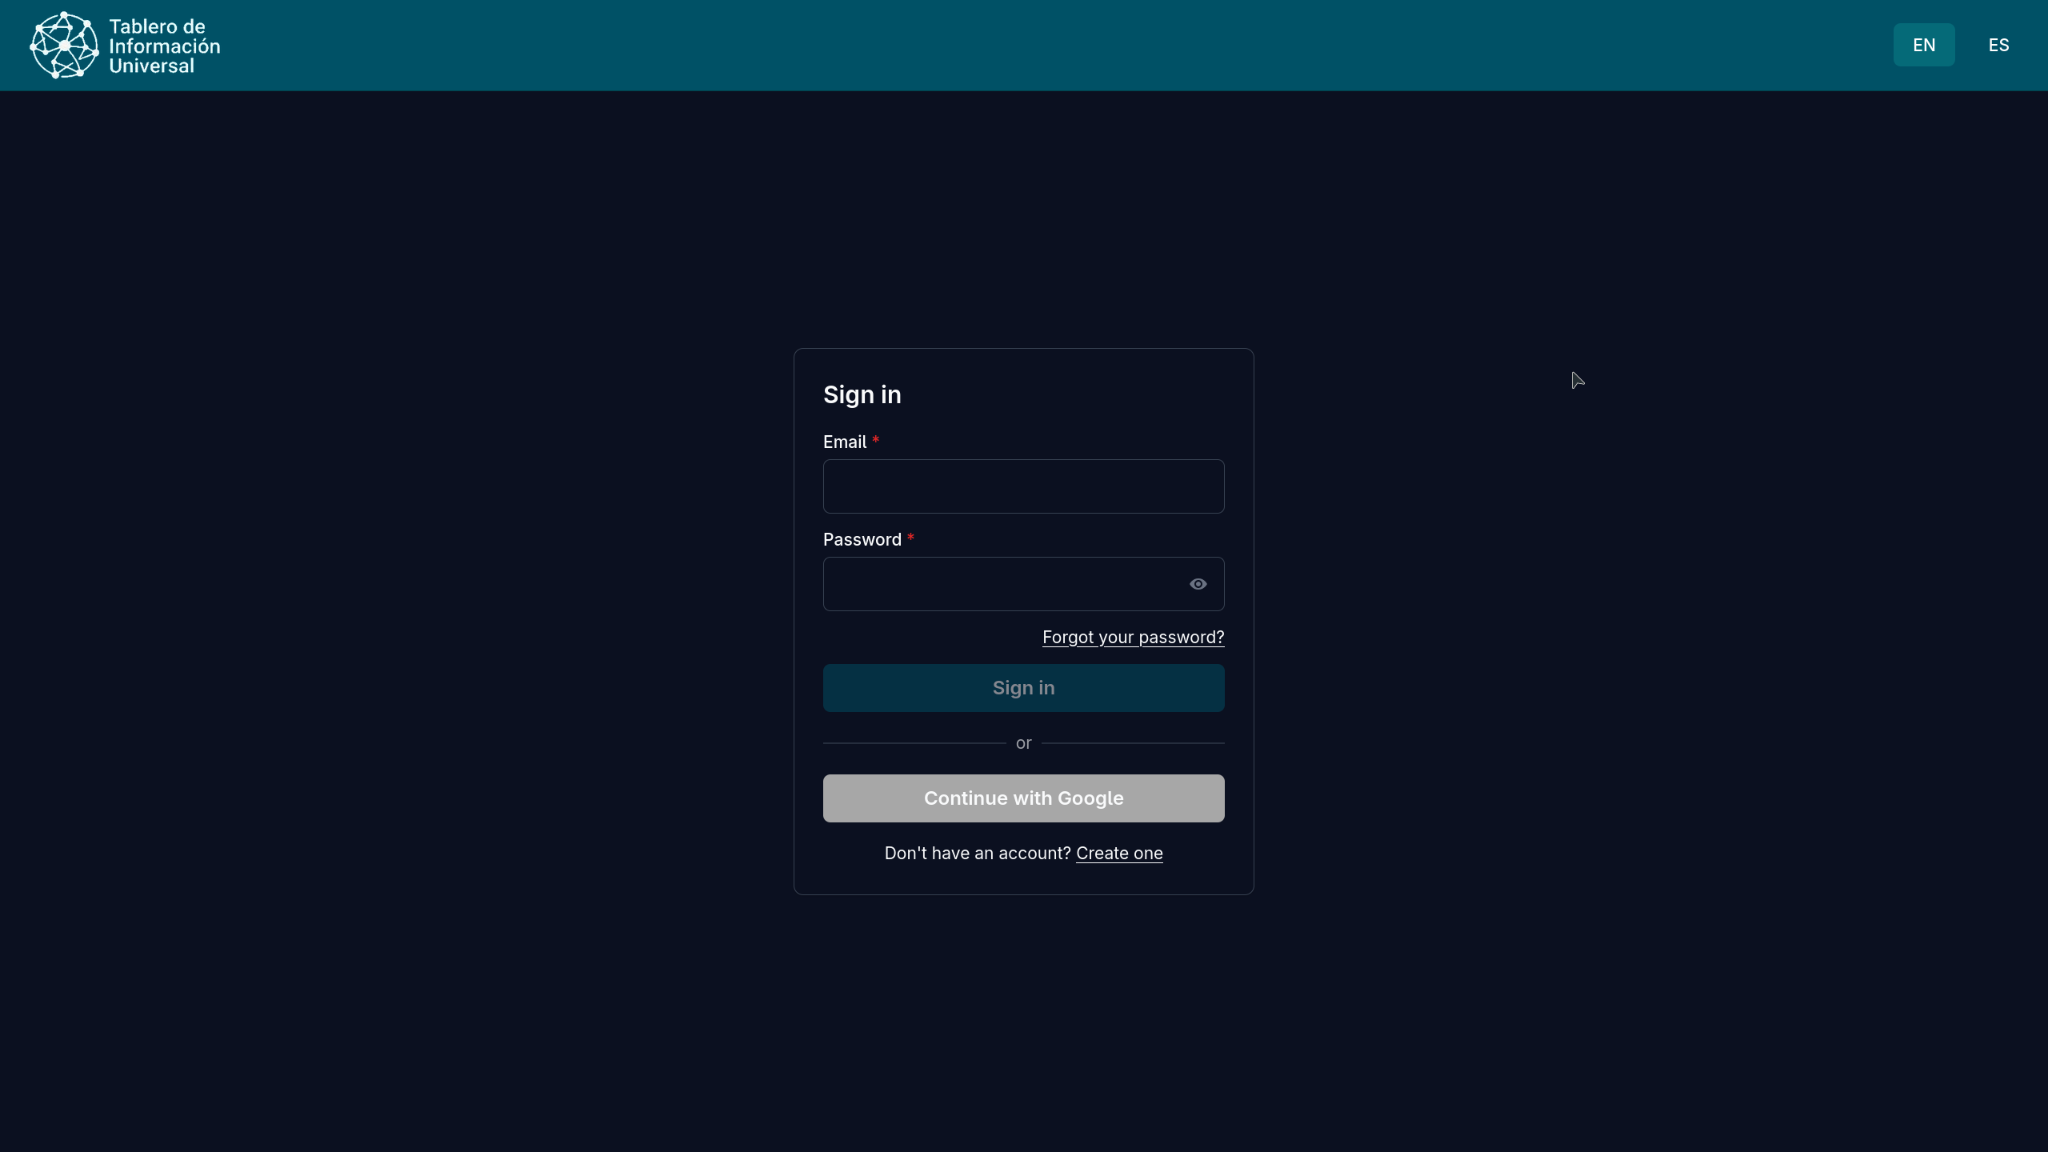
\includegraphics[width=0.92\textwidth]{figuras/fig28.png}
  \caption{Inicio de sesión en la web}
  \label{fig:ui_login}
\end{figure}

\begin{figure}[H]
  \centering
  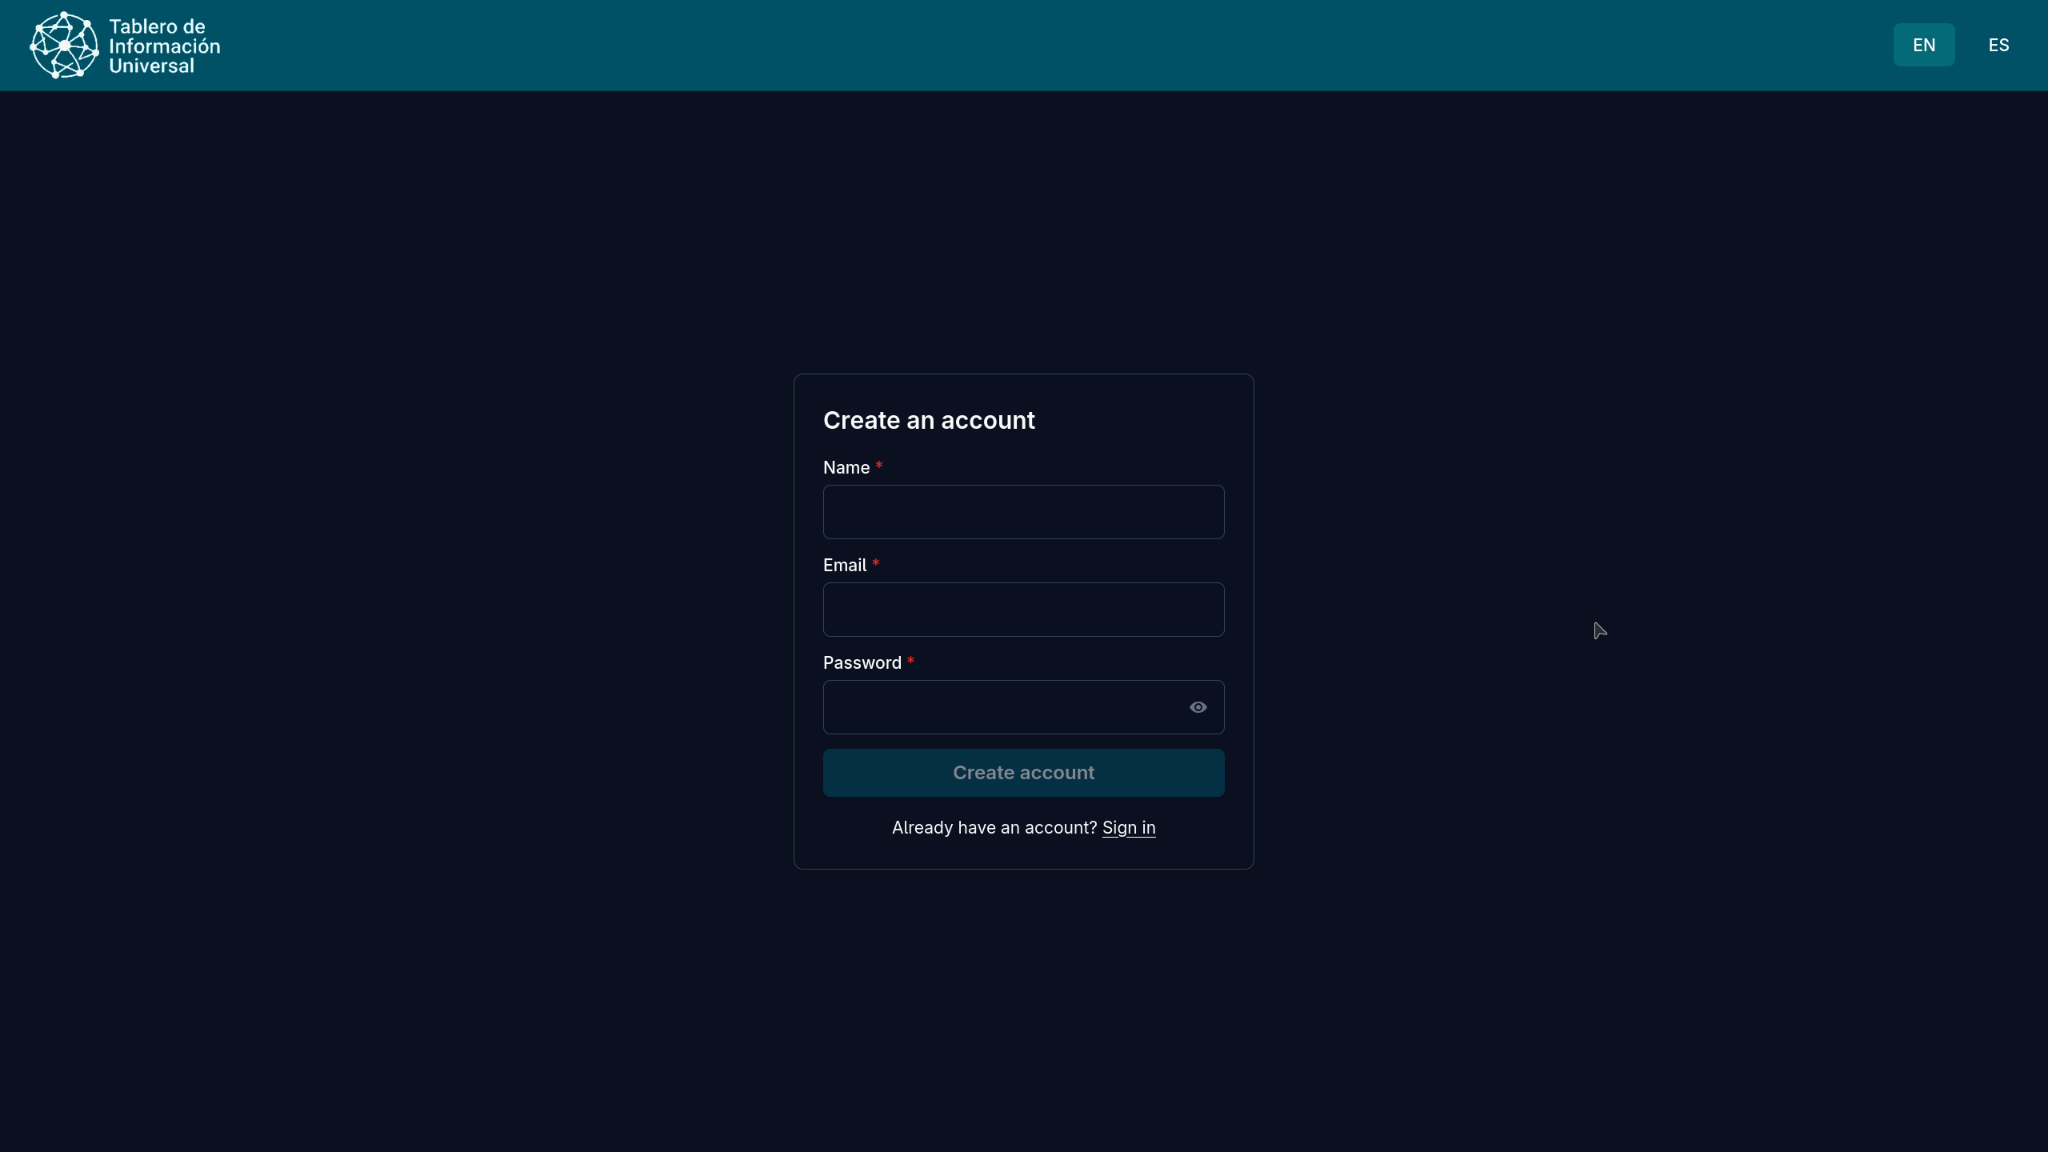
\includegraphics[width=0.92\textwidth]{figuras/fig29.png}
  \caption{Creación de cuenta}
  \label{fig:ui_registro}
\end{figure}

Una vez dentro, el usuario crea tableros desde la pantalla de inicio indicando su nombre; cada tablero nuevo pertenece a la organización seleccionada en ese momento, o al espacio personal del usuario (RF-04). La Figura~\ref{fig:ui_crear_tablero} presenta el formulario de creación.

\begin{figure}[H]
  \centering
  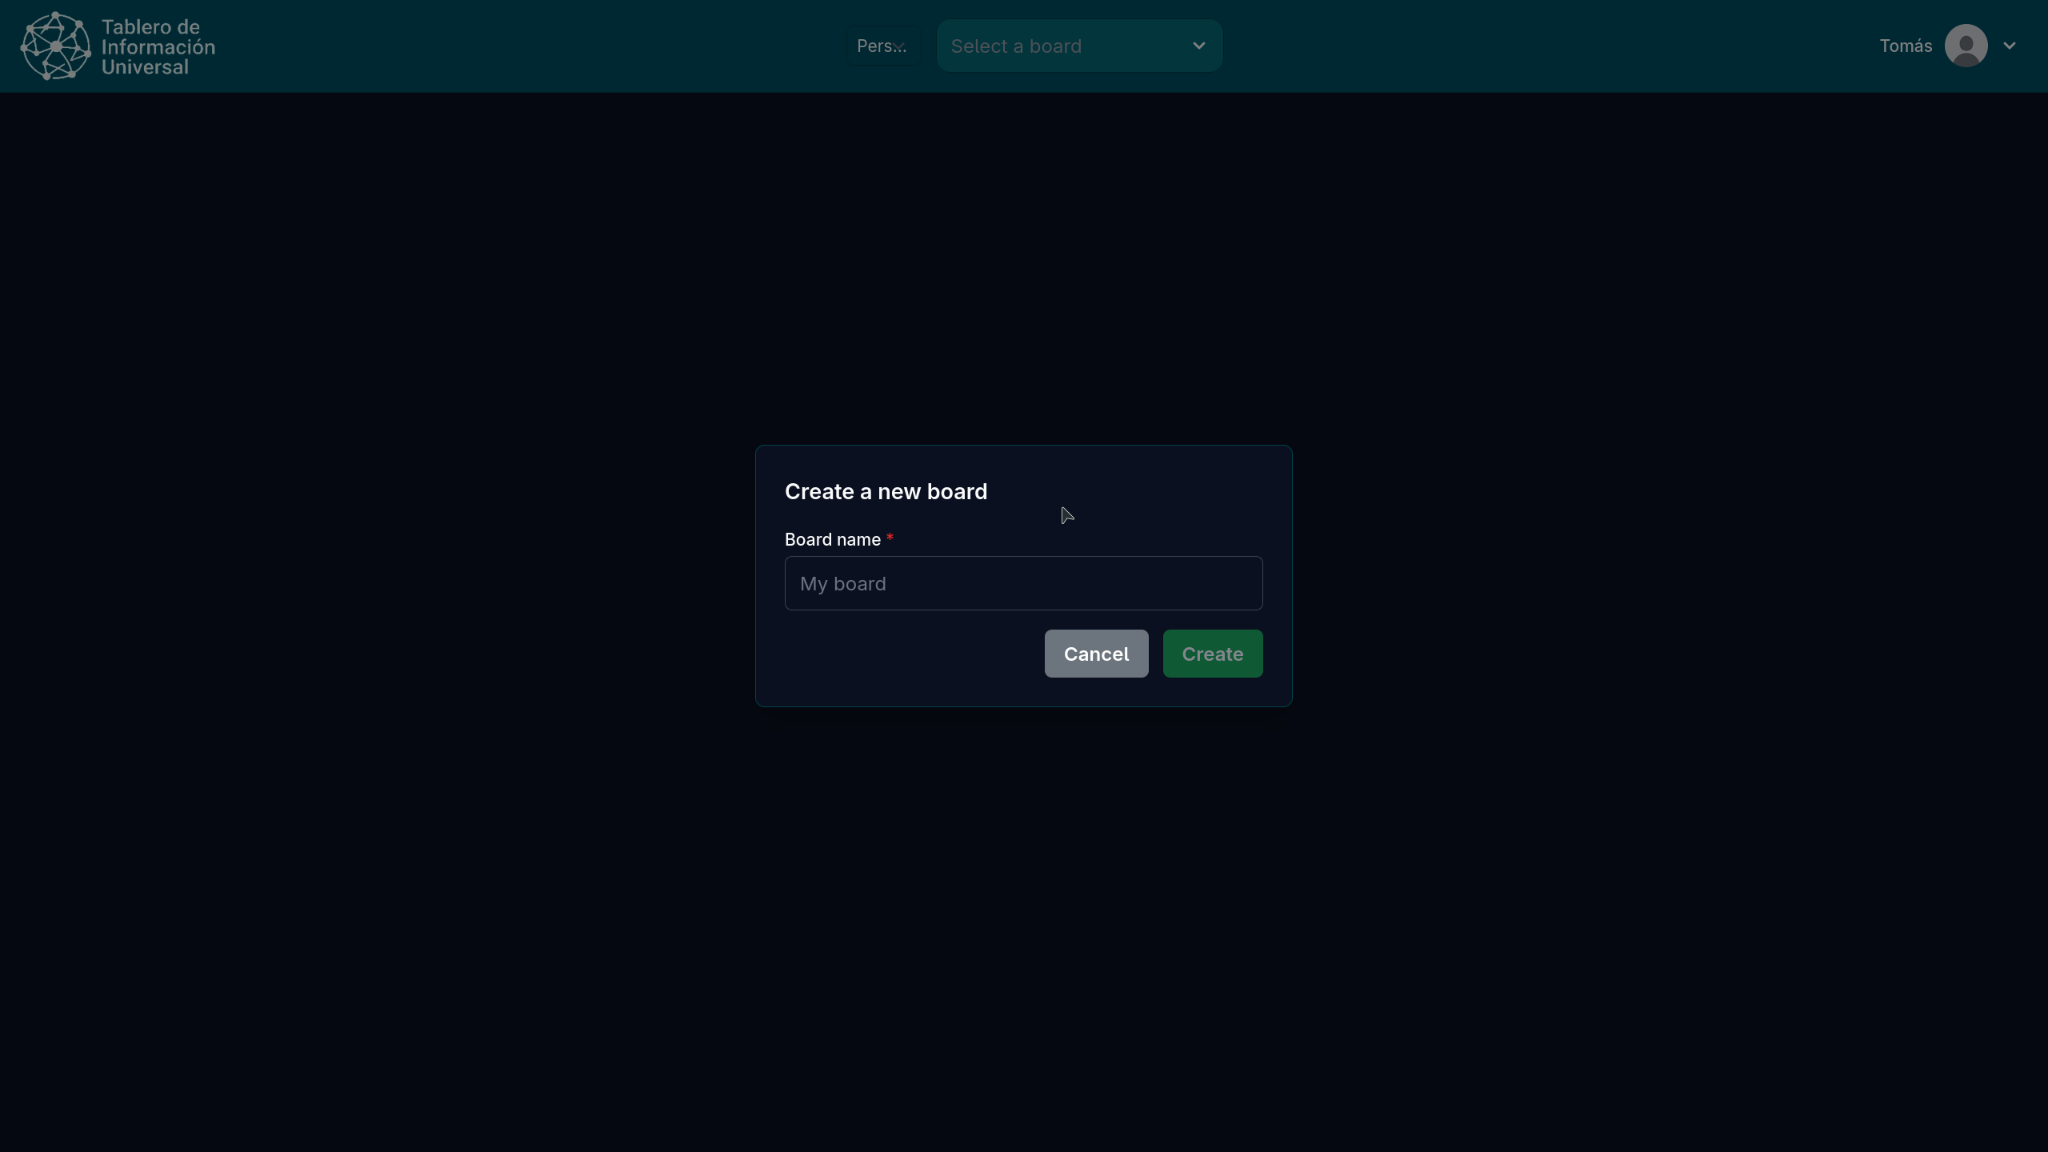
\includegraphics[width=0.92\textwidth]{figuras/fig30.png}
  \caption{Crear un tablero}
  \label{fig:ui_crear_tablero}
\end{figure}

Las tarjetas se agregan desde un carrusel que reúne las integraciones del catálogo y las plantillas disponibles en el tablero (RF-05 y RF-07). Al elegir una, el usuario completa sus variables configurables, como el repositorio en el caso de la tarjeta de GitHub, y la tarjeta se ubica en el lienzo, donde puede conectarse con otras mediante hilos (RF-06). Las Figuras~\ref{fig:ui_carrusel} a \ref{fig:ui_multiples_tarjetas} ilustran este recorrido.

\begin{figure}[H]
  \centering
  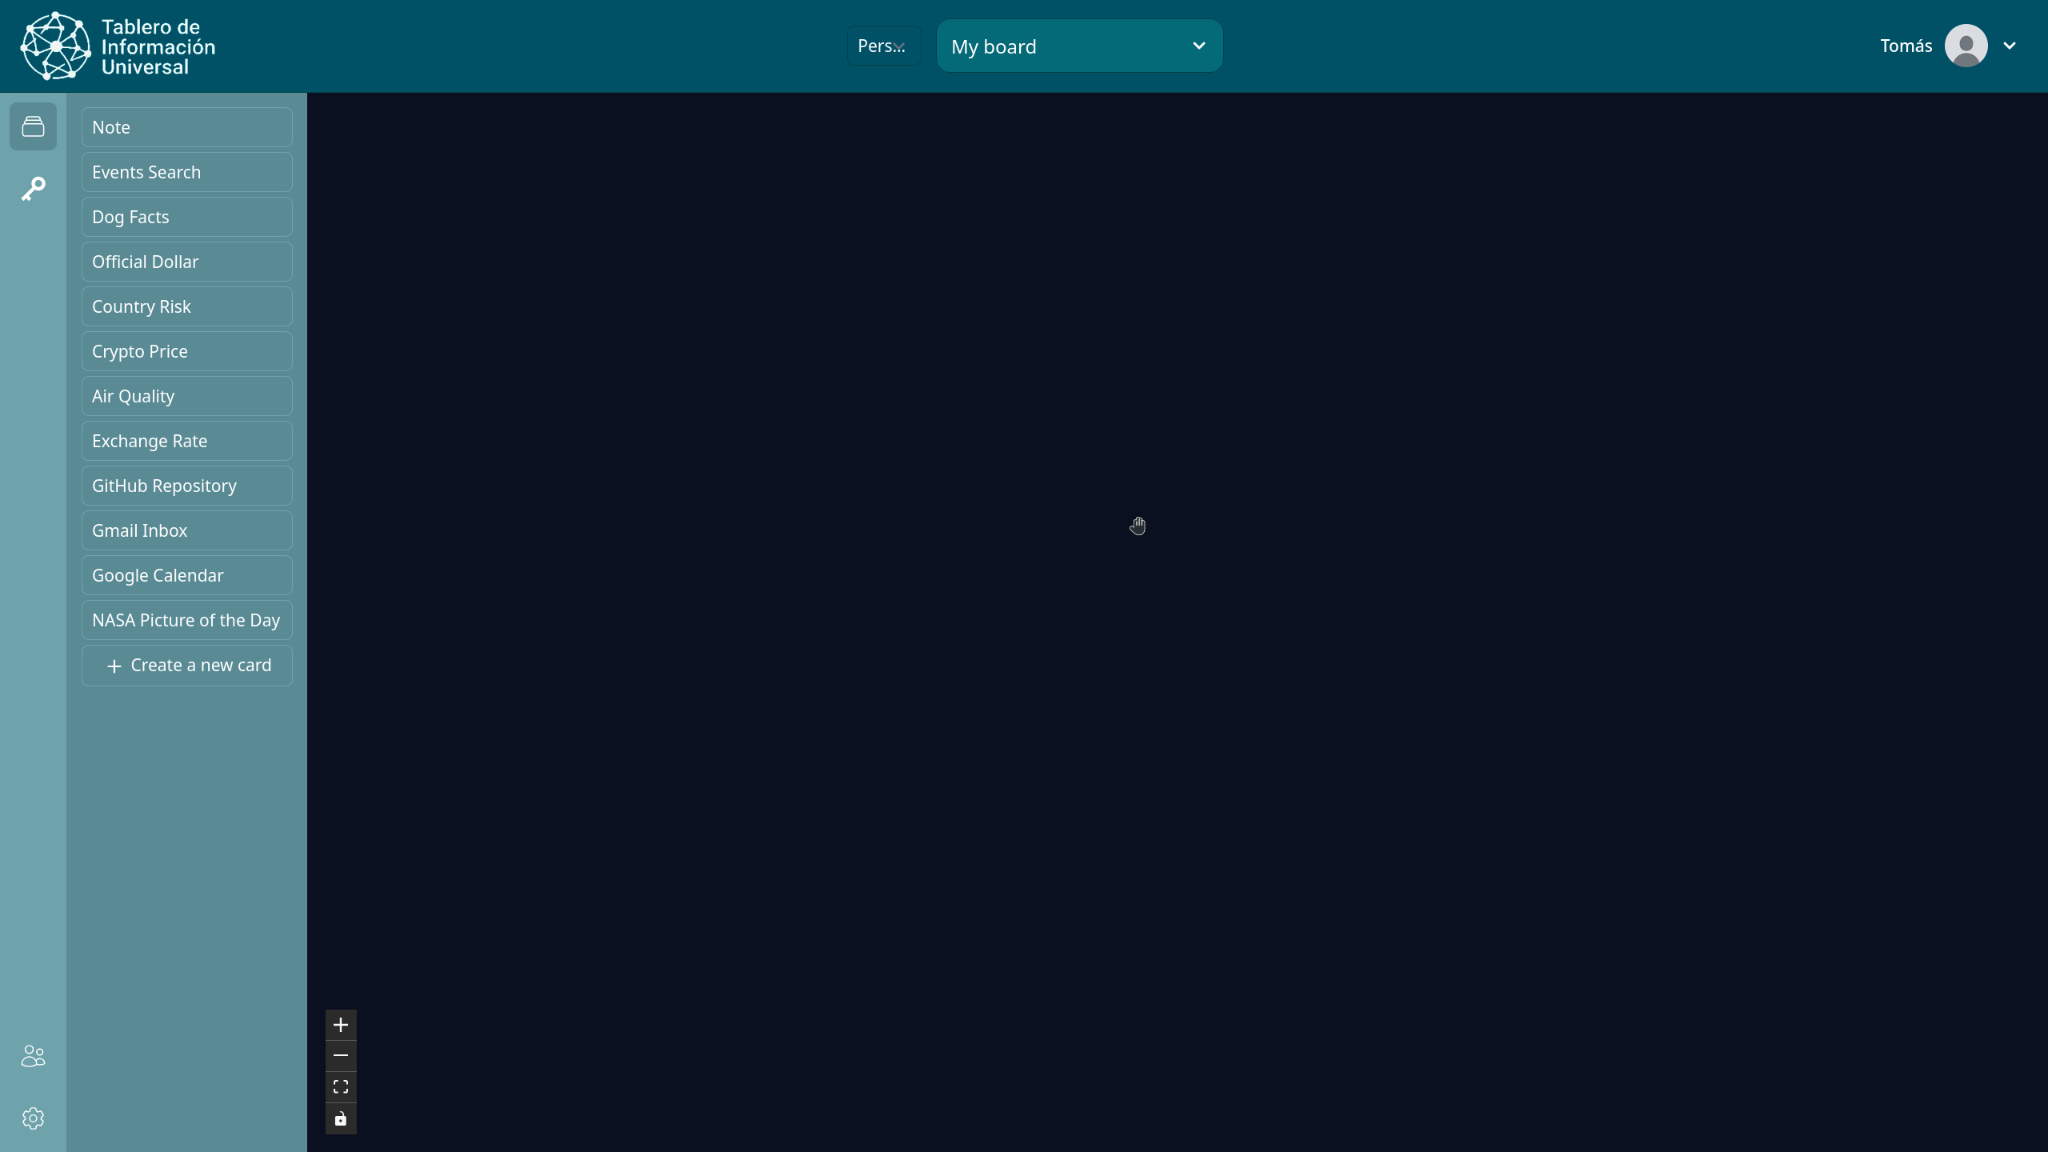
\includegraphics[width=0.92\textwidth]{figuras/fig31.png}
  \caption{Carrusel de tarjetas configurables}
  \label{fig:ui_carrusel}
\end{figure}

\begin{figure}[H]
  \centering
  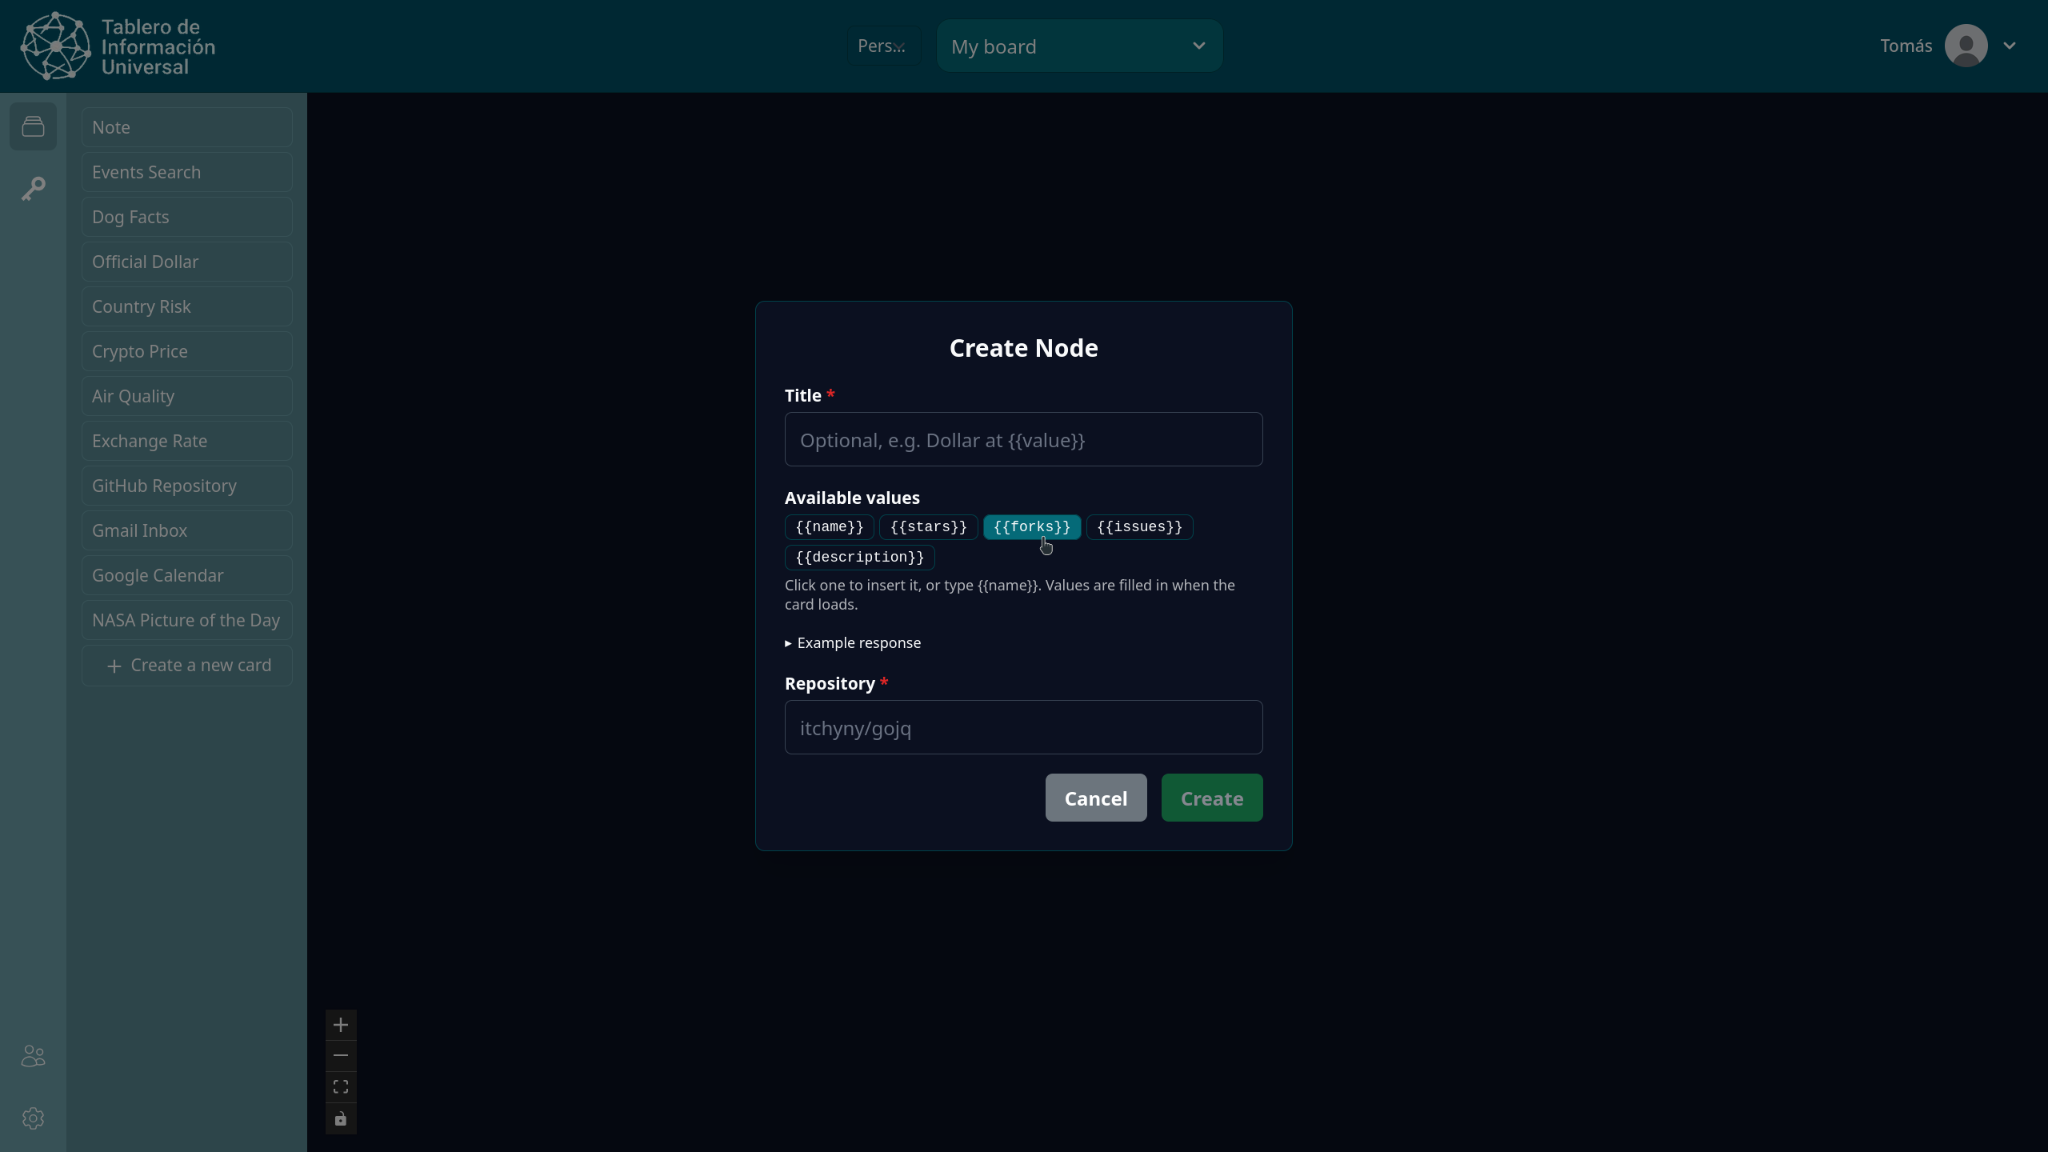
\includegraphics[width=0.92\textwidth]{figuras/fig32.png}
  \caption{Creación de tarjeta github - seleccionando variables configurables}
  \label{fig:ui_crear_github}
\end{figure}

\begin{figure}[H]
  \centering
  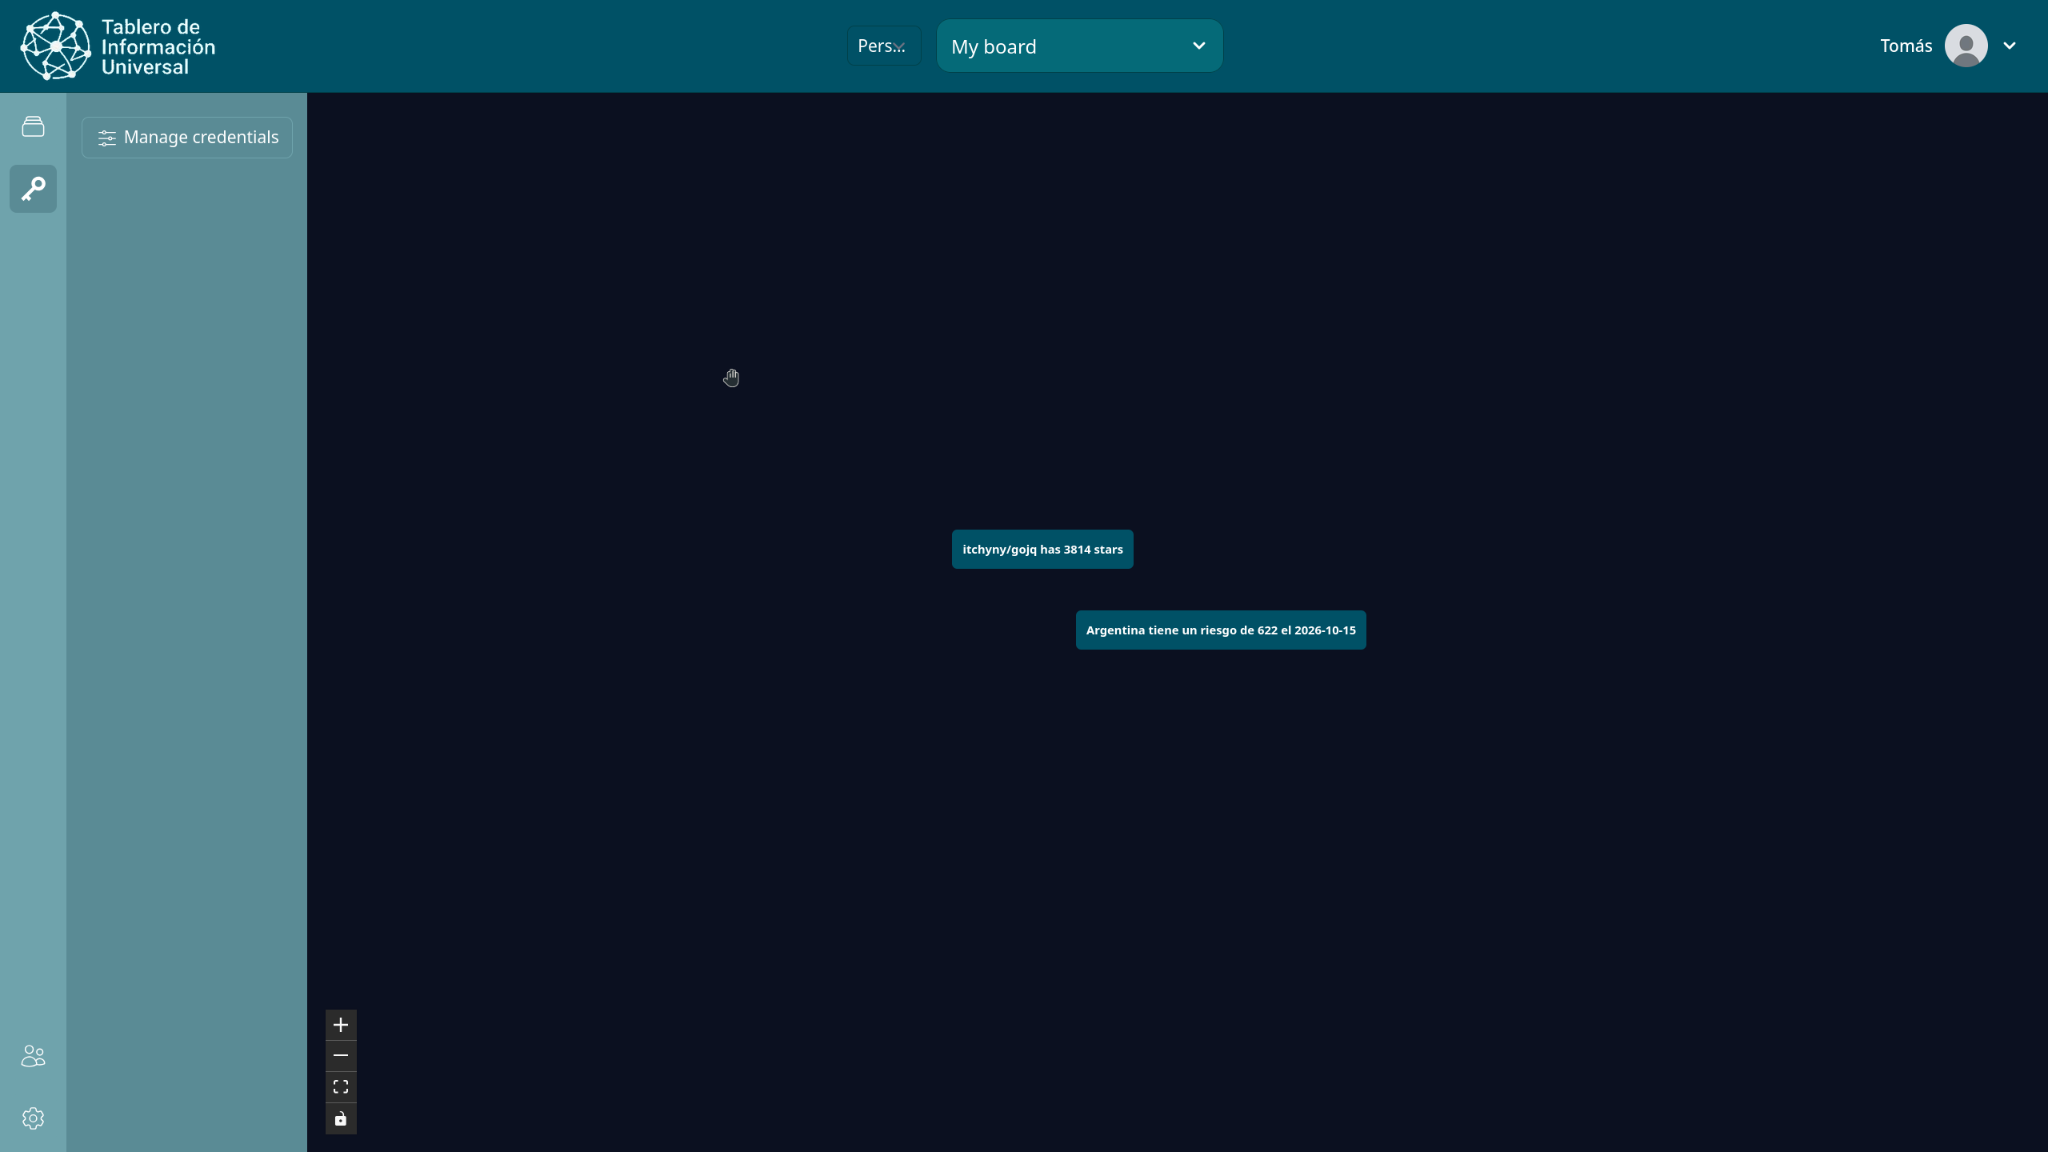
\includegraphics[width=0.92\textwidth]{figuras/fig33.png}
  \caption{Multiples tarjetas en un tablero y el carrusel de secretos}
  \label{fig:ui_multiples_tarjetas}
\end{figure}

Las integraciones que requieren autenticación toman sus credenciales del gestor de secretos del tablero, que permite cargar claves de API o conectar una cuenta externa mediante OAuth2. Al crear una tarjeta de este tipo, el formulario ofrece las credenciales que el usuario puede utilizar. Las Figuras~\ref{fig:ui_gestor_secretos} a \ref{fig:ui_nodo_credencial} muestran el gestor de secretos y la selección de una credencial.

\begin{figure}[H]
  \centering
  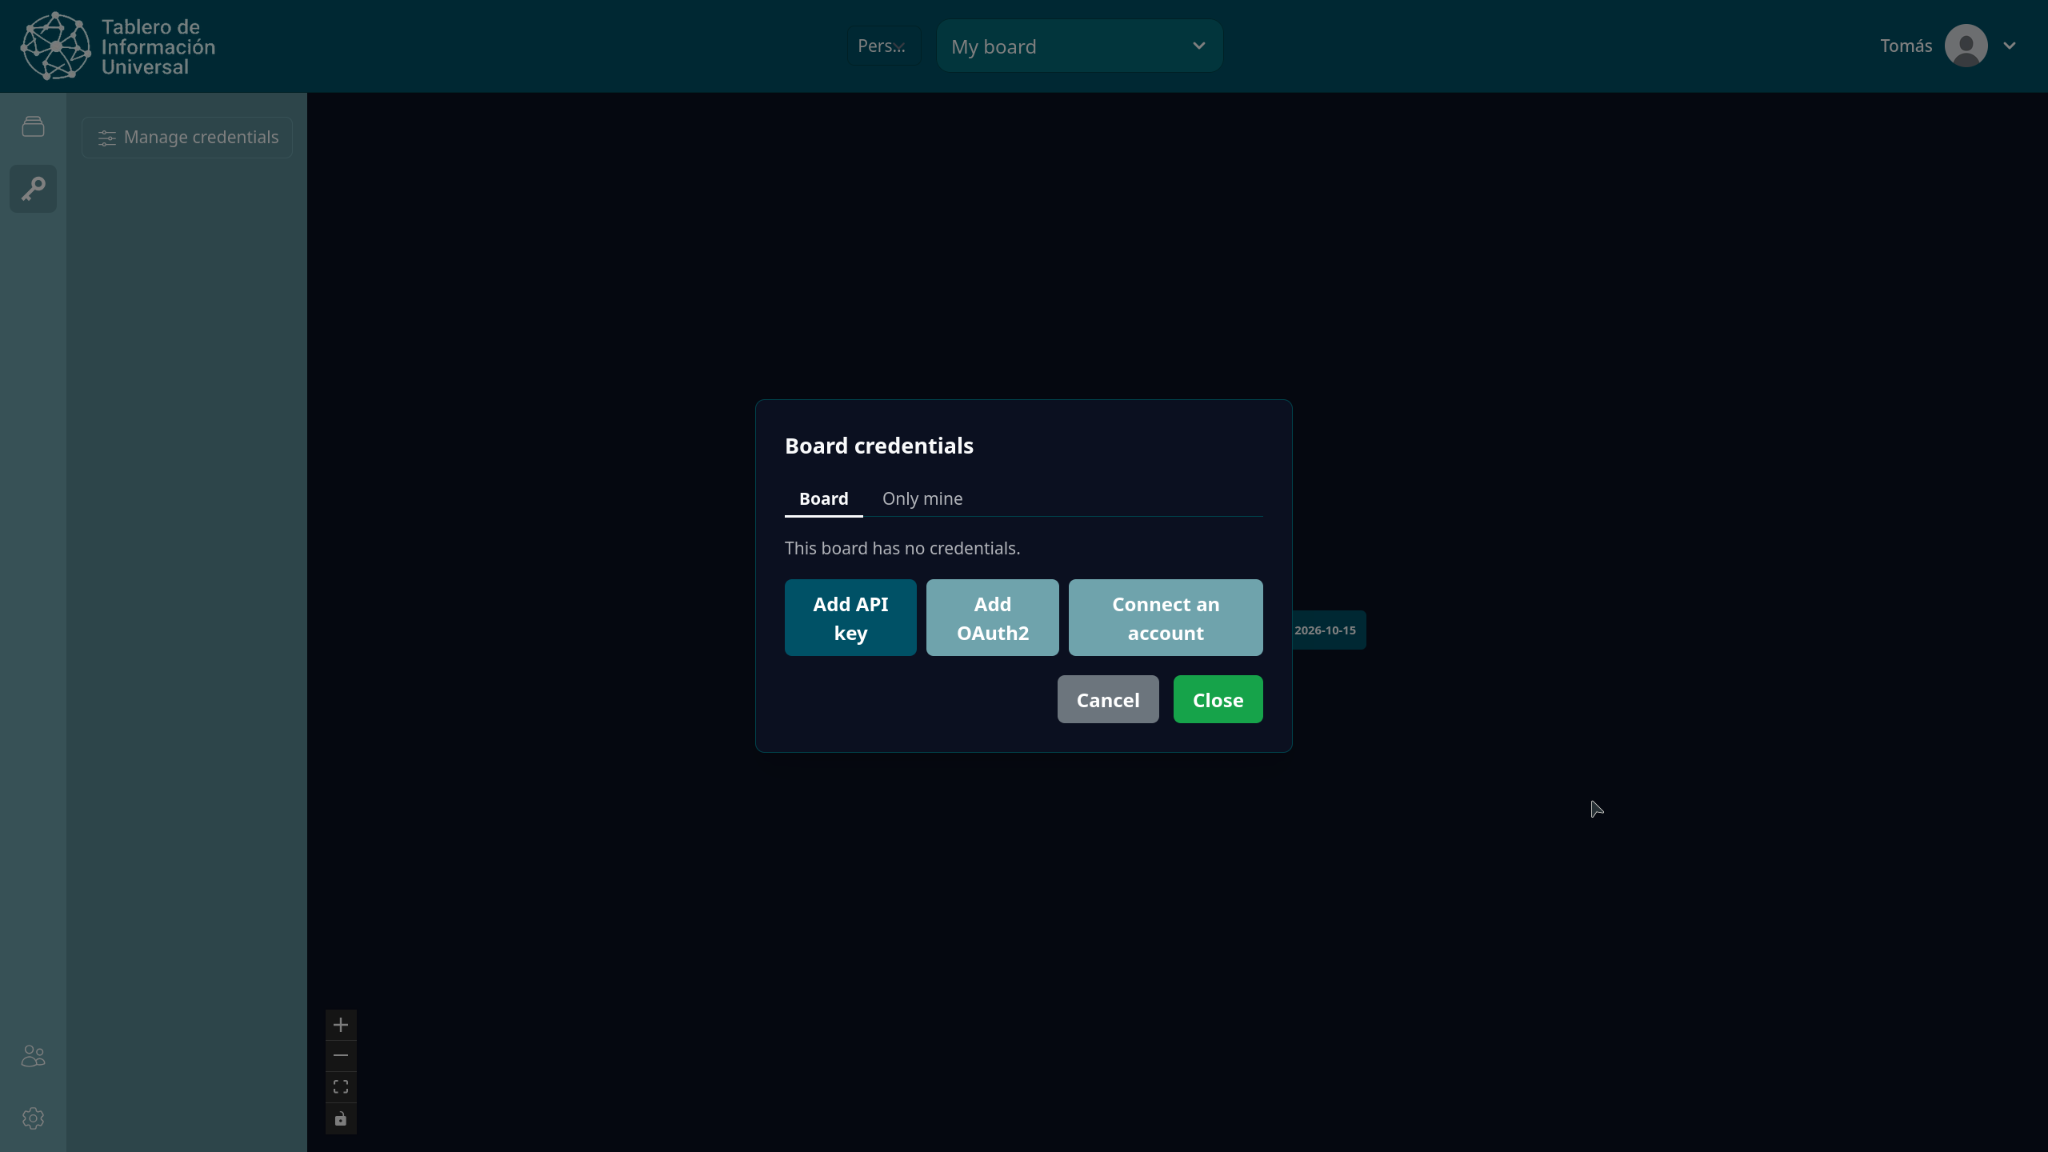
\includegraphics[width=0.92\textwidth]{figuras/fig34.png}
  \caption{Gestor de secretos del tablero}
  \label{fig:ui_gestor_secretos}
\end{figure}

\begin{figure}[H]
  \centering
  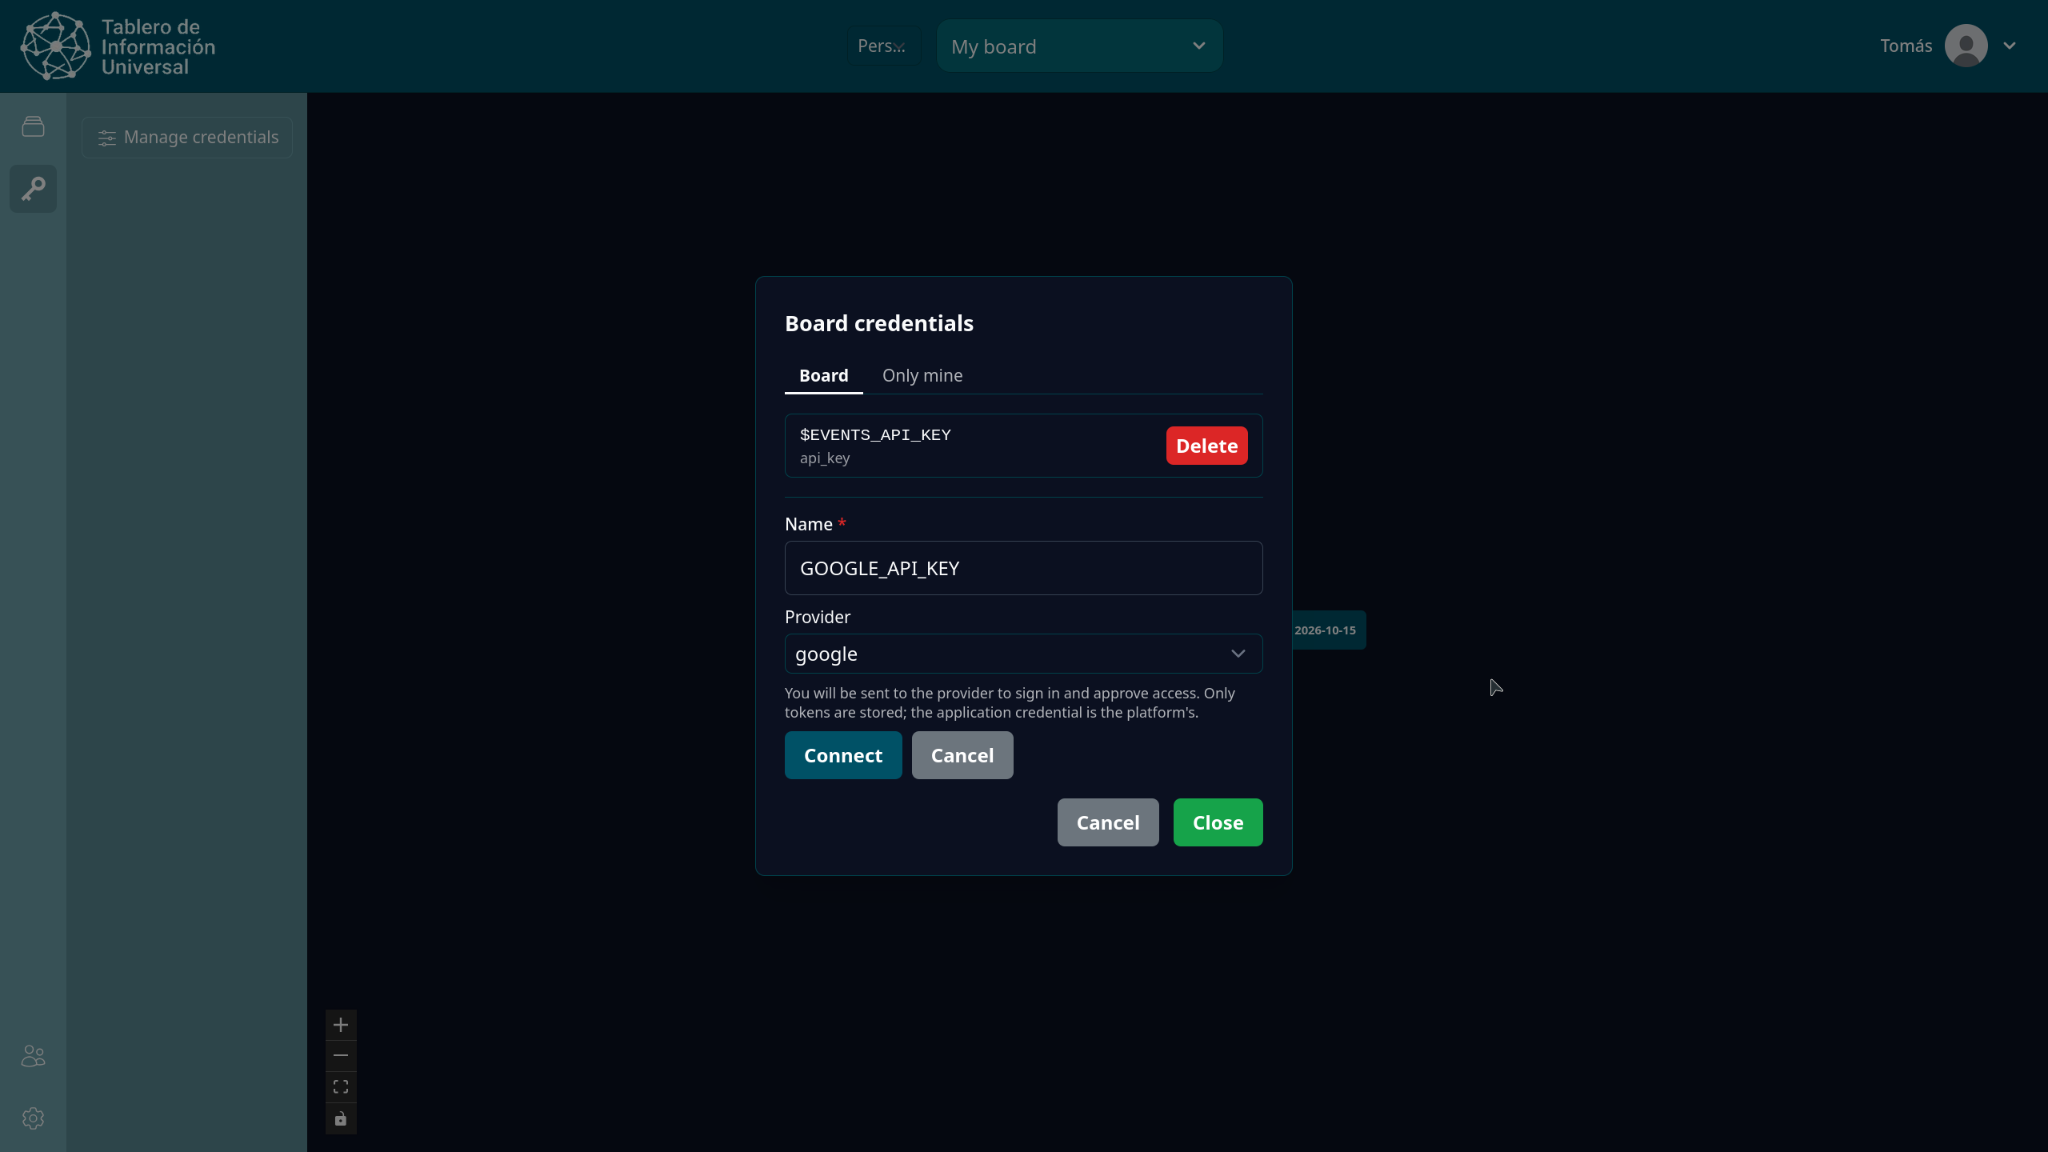
\includegraphics[width=0.92\textwidth]{figuras/fig35.png}
  \caption{Gestor de secretos, sumando una conexión OAuth}
  \label{fig:ui_oauth_secreto}
\end{figure}

\begin{figure}[H]
  \centering
  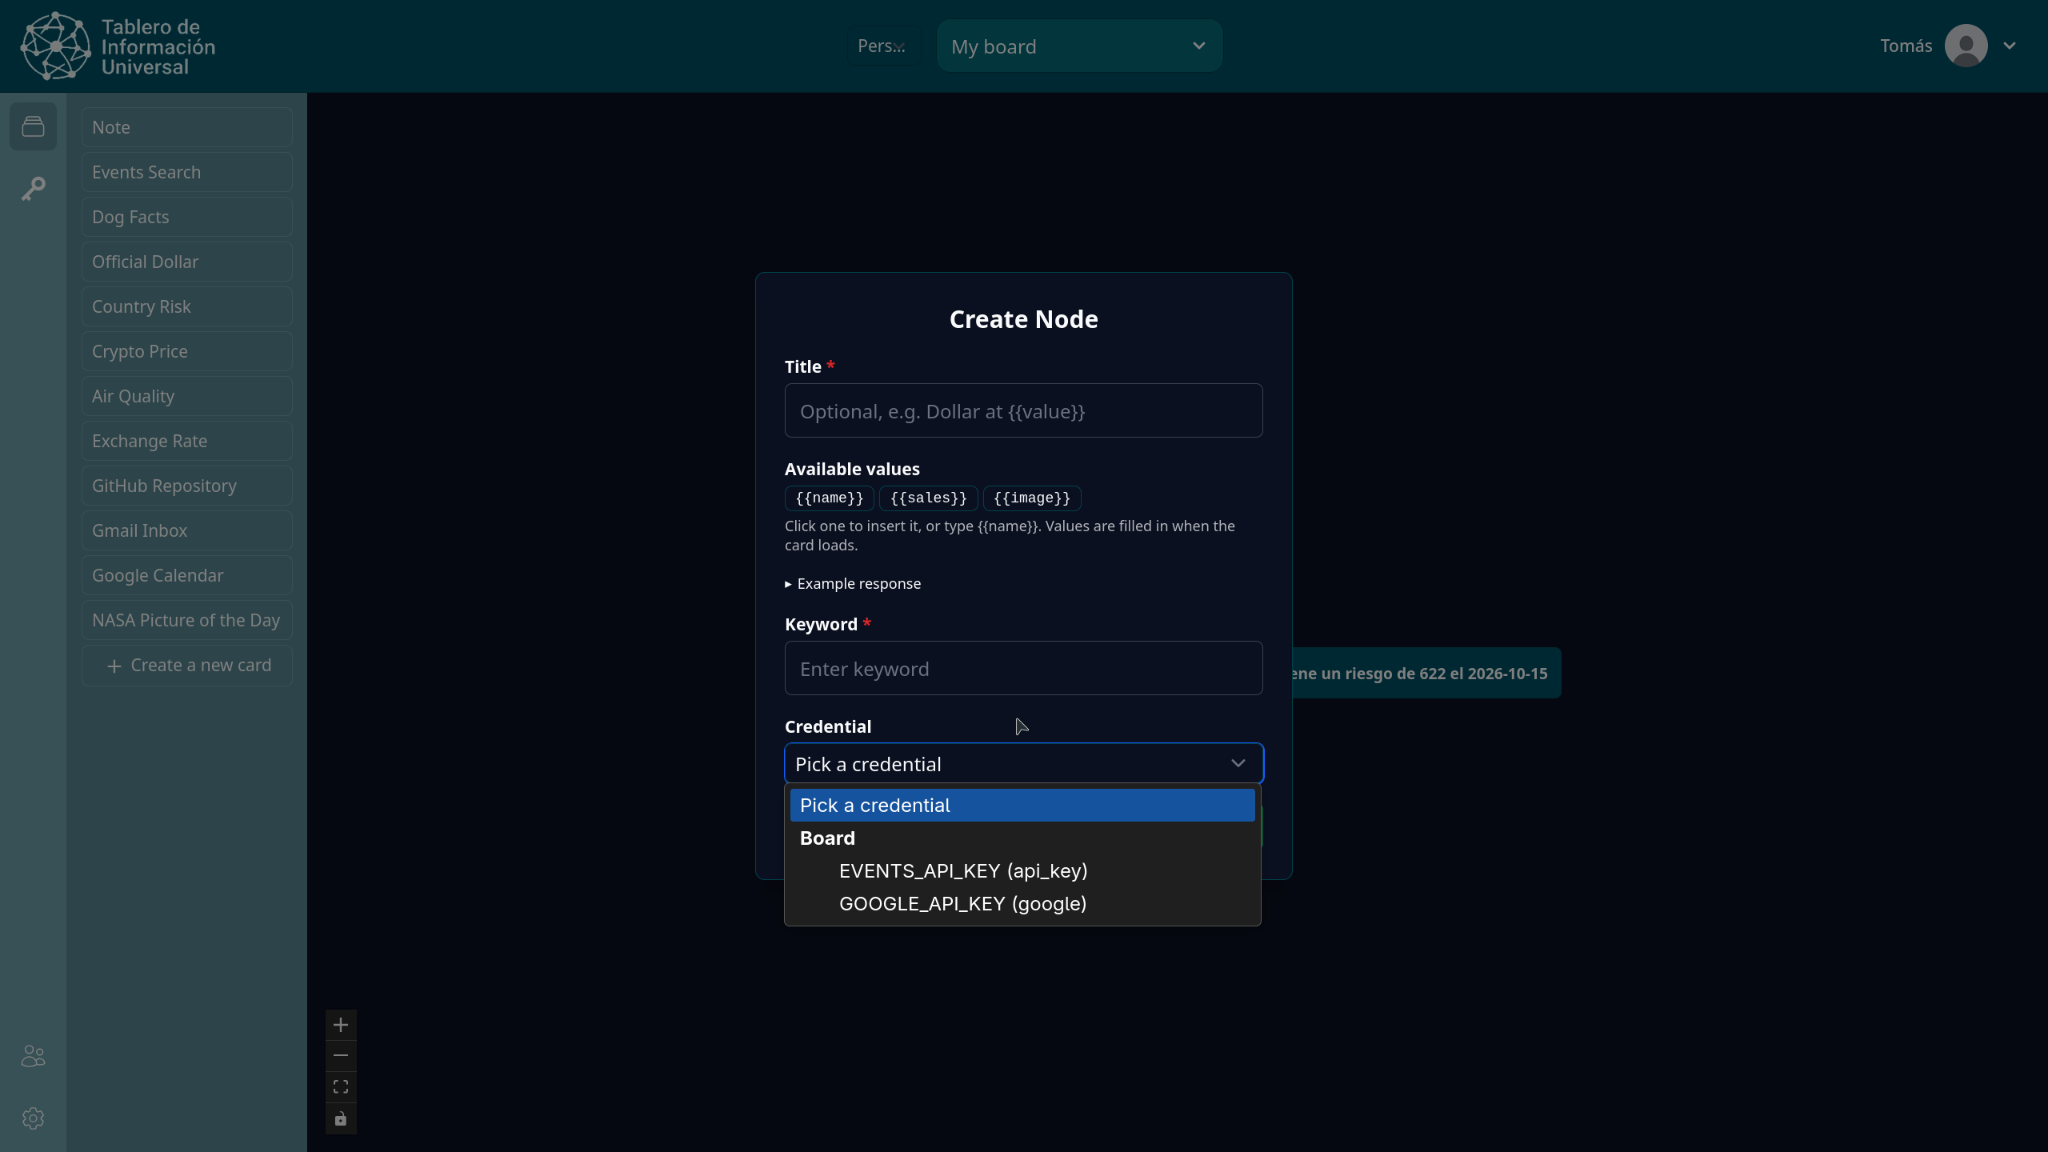
\includegraphics[width=0.92\textwidth]{figuras/fig36.png}
  \caption{Creación de nodo que requiere una credencial}
  \label{fig:ui_nodo_credencial}
\end{figure}

Por último, el dueño de un tablero puede compartirlo por email, asignando a cada persona el rol de editor o de lector (RF-13), y la pantalla de inicio reúne todos los tableros a los que el usuario tiene acceso. Desde el perfil, el usuario modifica sus datos y gestiona los tokens personales con los que se conectan herramientas externas, como el servidor MCP (RF-10). Las Figuras~\ref{fig:ui_compartir} a \ref{fig:ui_perfil} corresponden a estas pantallas.

\begin{figure}[H]
  \centering
  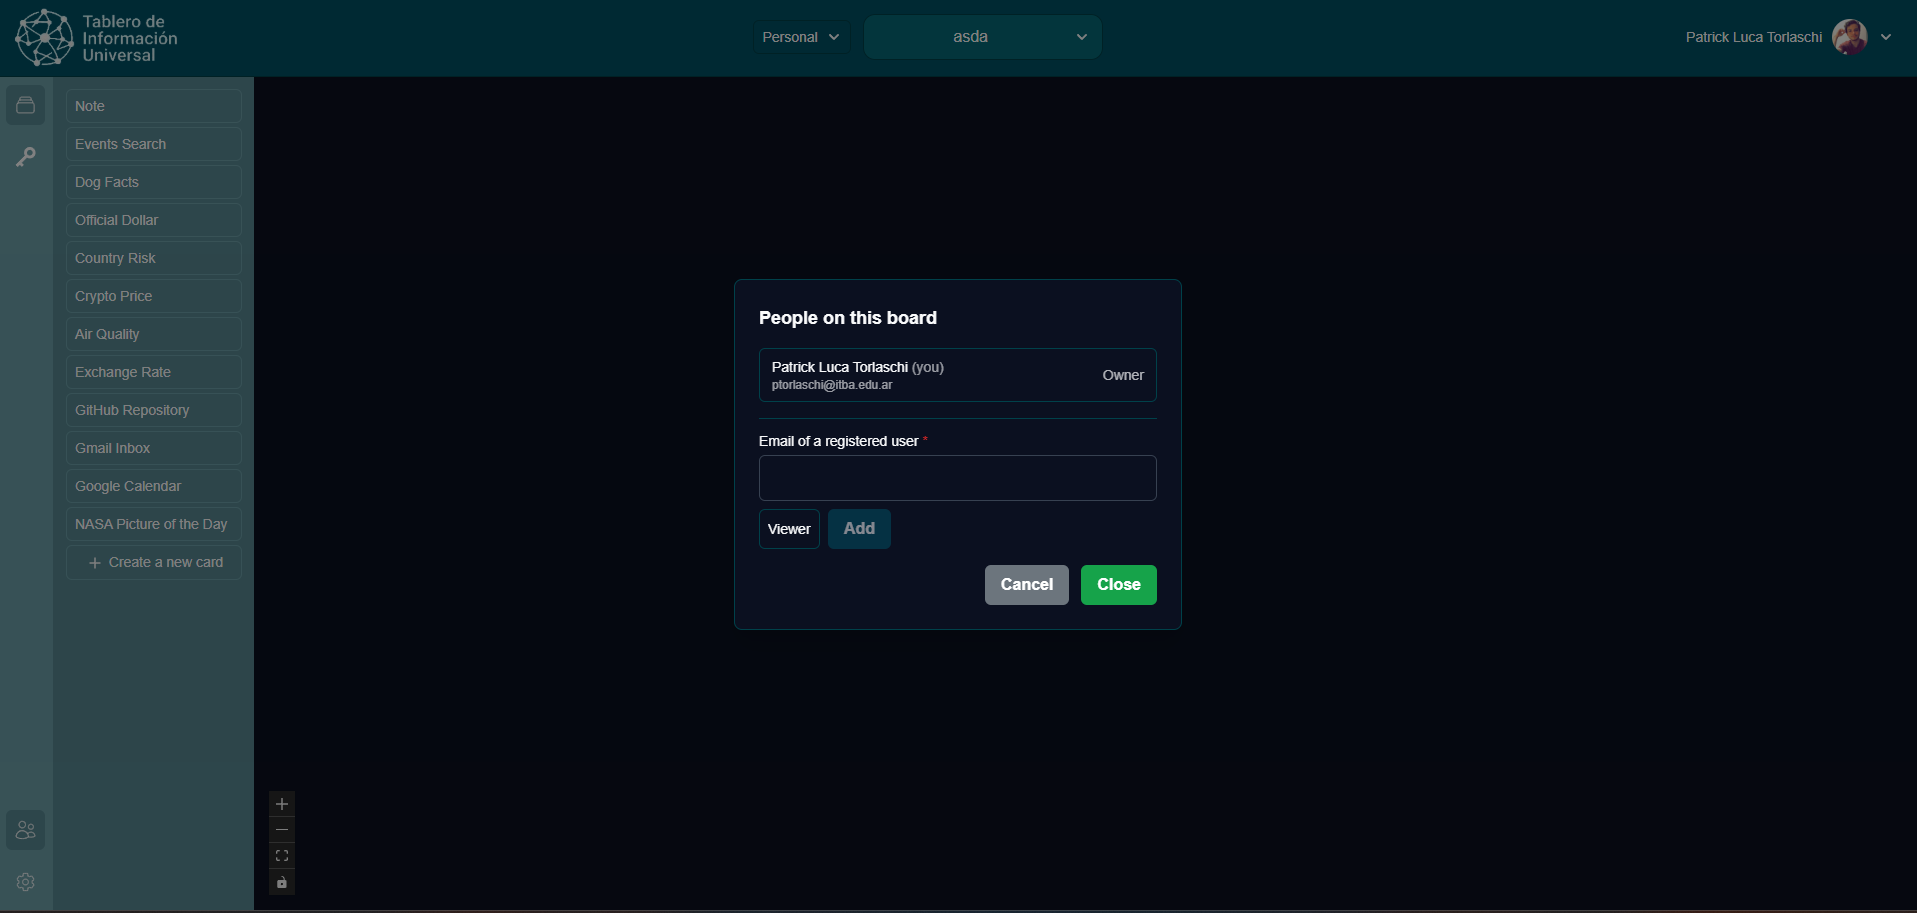
\includegraphics[width=0.92\textwidth]{figuras/fig37.png}
  \caption{Vista de compartir tablero}
  \label{fig:ui_compartir}
\end{figure}

\begin{figure}[H]
  \centering
  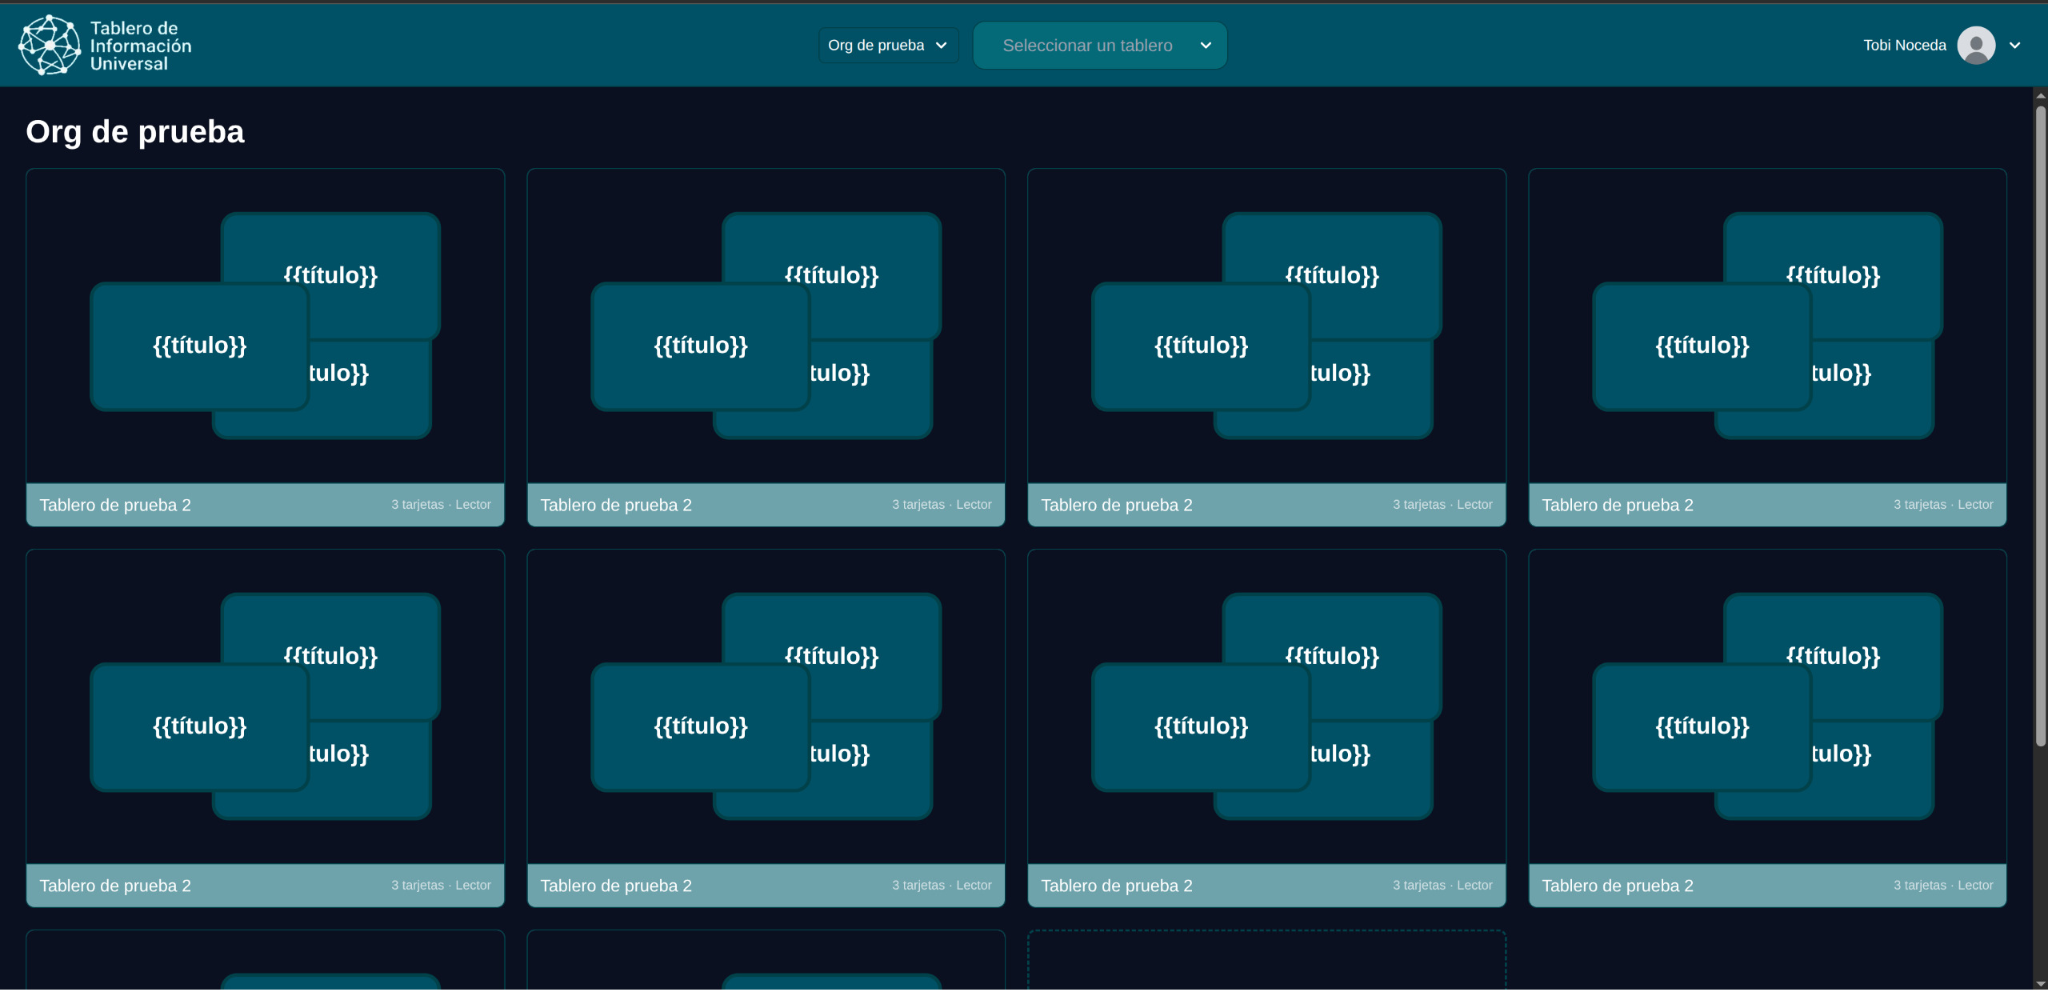
\includegraphics[width=0.92\textwidth]{figuras/fig38.png}
  \caption{Vista de inicio con varios tableros}
  \label{fig:ui_inicio_tableros}
\end{figure}

\begin{figure}[H]
  \centering
  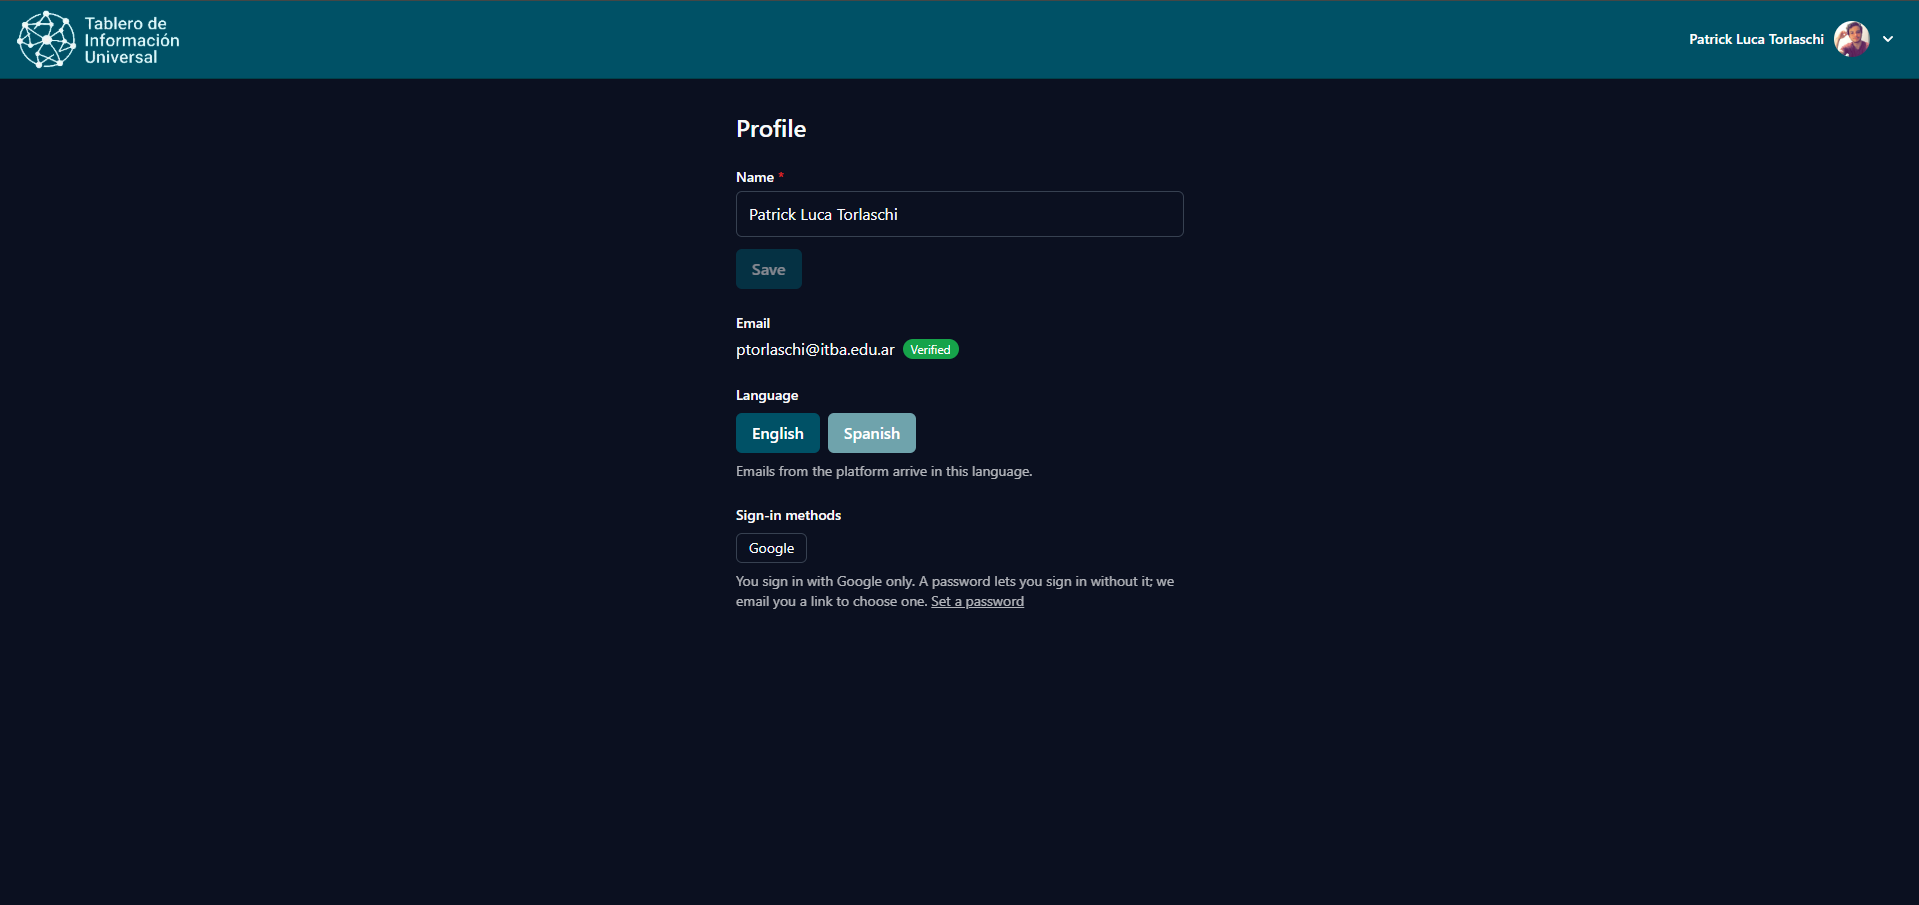
\includegraphics[width=0.92\textwidth]{figuras/fig39.png}
  \caption{Vista del perfil de usuario}
  \label{fig:ui_perfil}
\end{figure}

% 4. Bibliografía IEEE ordenada automáticamente por aparición
\clearpage
\addcontentsline{toc}{chapter}{Bibliografía}
\printbibliography[title={Bibliografía}]

% 5. Reconocimiento y Agradecimientos
% !TEX root = ../main.tex
\chapter*{Agradecimientos}
\addcontentsline{toc}{chapter}{Agradecimientos}

Queremos agradecer a todos nuestros familiares y amigos, quienes nos acompañaron en el desarrollo del sistema, ofreciendo sugerencias de mejora o alternativas, y por haber participado en las pruebas de HCI, haya sido voluntaria o involuntariamente.


\end{document}